\documentclass{osudissert96}

%%%%%
% start custom preamble lines
%%%%%
\usepackage[T1]{fontenc}
\usepackage{amssymb}
\usepackage{amsmath}
\usepackage{graphicx}
%since overleaf frequently times out
%typically need to compile with draft mode on, then without draft
%\usepackage[draft]{graphicx}
\usepackage{ragged2e}
\usepackage{bigstrut}
\usepackage{colortbl}
\usepackage{arydshln}
\usepackage{subcaption}
\usepackage{caption}
\captionsetup[figure]{font=small,labelfont=small}
\usepackage{float}
\usepackage{enumitem}
\usepackage{algpseudocode}
\usepackage[chapter]{algorithm}
\usepackage{textcomp}
\usepackage{soul}
\usepackage{ascii}
\usepackage{comment}
%it's 2021, and I prefer biber/biblatex over bibtex
\usepackage[backend=biber,
style=trad-plain,
citestyle=numeric-comp,
sorting=none,
maxbibnames=6,
minbibnames=6
]{biblatex}
\usepackage[letterpaper,margin=1in,includefoot]{geometry}
\usepackage{pdflscape}
%causes a problem with accent in \member unless T1 encoding used
%protrusion disabled since we need to strictly follow 1 inch margins
\usepackage[stretch=10,shrink=10,protrusion=false]{microtype}
%\usepackage{todonotes}
\usepackage[hidelinks,setpagesize=false]{hyperref}
\pdfstringdefDisableCommands{%
  \let\enspace\empty  % this causes the warning for \kern
  \let\noindent\empty % this causes the warning for \indent
  \let\kern\empty%
  \def\hbox#1{<#1>}%
  \def\lower#1{<#1>}%
}
%hide bookmarks bar by default in PDF viewers
\hypersetup{pdfpagemode=UseNone}

%number subsubsections for easier cross-refs
\setcounter{secnumdepth}{3}

%stay within 1in left margin
%https://tex.stackexchange.com/questions/398621/how-to-left-align-enumerate-labels-at-the-left-margin
\setlist[enumerate]{wide=0pt, widest=99,leftmargin=\parindent, labelsep=*}

\addbibresource{refs.bib}

%for vita
\newcommand*{\cofirst}[0]{\textsuperscript{*}}
\newcommand*{\pmid}[1]{\underline{\href{https://pubmed.ncbi.nlm.nih.gov/#1/}{#1}}}

%for 240
%using \def to avoid t1 issues and whether or not something else defines \textapprox
\def\textapprox{\raisebox{0.5ex}{\texttildelow}}

\DeclareMathOperator{\vaf}{VAF}

\newcommand*{\mtpose}{^{\mathsf{T}}}

\newcommand*{\twodots}{\mathinner {\ldotp \ldotp}}

%for 303
\DeclareMathOperator*{\argmax}{argmax}
\DeclareMathOperator{\cov}{Cov}

%for SCLC
\DeclareMathOperator{\pBinom}{pBinom}
\DeclareMathOperator{\pNorm}{p\mathcal{N}}
\DeclareMathOperator{\Uniform}{Uniform}

%for MSI clones
\DeclareMathOperator{\sse}{SSE}


\algnewcommand{\IfThenElse}[3]{% \IfThenElse{<if>}{<then>}{<else>}
  \State \algorithmicif\ #1\ \algorithmicthen\ #2\ \algorithmicelse\ #3}

\algnewcommand{\IfThen}[2]{% \IfThen{<if>}{<then>}
  \State \algorithmicif\ #1\ \algorithmicthen\ #2}

\newcommand*{\ssig}{\textsuperscript{*}}
\newcommand*{\ssigg}{\ssig{}\ssig{}}
\newcommand*{\ssiggg}{\ssig{}\ssigg{}}


%%%%%
% end custom preamble lines
%%%%%

%
% To change the dissertation to a Master's Thesis, include a documentclass
% option such as [masters], [ms], [ma], etc.  Also available are [osudraft]
% and [twoside].  As a reminder, documentclass options are a
% comma-separated list, e.g. \documentclass[ms,osudraft]{osudissert96}
%

%
% Everything between the \documentclass and the \begin{document} is
% called the preamble of the document. Everything between the
% \begin{document} and the \end{document} is called the body of the
% document. Define any additional commands you want here (the preamble)
%

% BibTeX from the BiBTeX Documentation
%\def\BibTeX{{\rm B\kern-.05em{\sc i\kern-.025em b}\kern-.08em
%    T\kern-.1667em\lower.7ex\hbox{E}\kern-.125emX}}

%
% It is better to break up the dissertation into multiple files (e.g.,
% one file per chapter, as well as separate files for the abstract,
% acknowledgements, and vita).  These files are brought into the
% document using \include{} statements.  There will be times, however,
% when you don't want to print the ENTIRE dissertation.  You can limit
% what will actually be printed by using the \includeonly{} statment.
% This contains a list of the files you want printed.  Any file NOT
% listed will not be printed.  However, all page numbers, references,
% etc., will be preserved as though all the files were actually
% printed. For example, the line below would result only in chapters 1
% and 3 being printed (if it were uncommented).
%

%\includeonly{ch1.intro,ch3.implem}

% UPDATED TEXT (2010):
%  In the newest format, titles should be title case everywhere.
%
% HISTORICAL TEXT (1996):
%  In the new format, the titles of each chapter should appear in
%  uppercase.  In the TOC, however, they should be in lowercase.
%  The command below automates this behavior.  However, you'll have to be
%  careful not to include \labels within your \chapter definitions or
%  there will be problems.  If you don't want this to be automated, comment
%  out the \typesetChapterTitle definition below and do your chapters in
%  the form:
%  \chapter[MY TITLE]{My Title}
%
%  \renewcommand\typesetChapterTitle[1]{\uppercase{#1}}
\renewcommand\typesetChapterTitle[1]{#1}

\begin{document}

%
% First, declare the parts of your title page 
%

\author{Russell Bonneville}
\title{Data-Driven Insights into Cancer as a Dynamic Process}
\authordegrees{B.S.}  % Degrees thus far, not including this one.
\unit{Biomedical Sciences}

\advisorname{Sameek Roychowdhury}
\member{Robert Baiocchi}
\member{Ewy A. Math\'{e}}
\member{Lang Li}
\member{Lianbo Yu}

%
% The following creates the title page
%

\maketitle

% Next, EITHER a copyright or BLANK page.
%
%   The following creates a page used to copyright your dissertation
%
%   BACKGROUND: Even without this copyright page, your dissertation will
%               carry a common-law copyright. However, if your
%               dissertation ends up seeing wide distribution, your
%               common-law copyright is at risk of being expunged.
%               Adding this copyright page prevents that from happening.
%
%               There are NO DOWNSIDES to including a copyright page as
%               your document is automatically copyright by law anyway.
%               However, this copyright page is OPTIONAL. If you get rid
%               of it, uncomment the \blankpage that follows it so that
%               there is a blank page here. The graduate school requires
%               a page here that is either blank or carries the
%               copyright.
%
%   IMPORTANT NOTE: The graduate school requires either a copyright page
%                   here or a BLANK PAGE here. If you get rid of the
%                   copyright, uncomment the \blankpage that follows it.
%                   You should NOT have BOTH uncommented.
%

% If you get rid of \disscopyright, restore the \blankpage line after it
\disscopyright
%\blankpage

%
% Abstract goes here.
%

\begin{abstract}
  %  The dissertation abstract can only be 500 words.

Cancers begin through acquisition of genomic alterations in normal cells, leading to uncontrolled cell division. However, cancer cells continue to accumulate alterations throughout the disease course. Therefore cancer in a patient is a continually changing entity subject to microevolution. This leads to tumor heterogeneity, or genetic diversity within a cancer case. Heterogeneity significantly complicates cancer diagnosis and treatment, as different cancer cells in the same patient may behave and respond differently. Current research and clinical paradigms of cancer inspect the disease at one or a few fixed time points, for instance at a patient's oncologist visits. Furthermore, most clinical and research assays of cancer in patients analyze only the small subsets of cancer cells obtained through singular biopsies. Through studying mutation and heterogeneity, we can formulate models of cancer as the dynamic process that it is, and explore the temporal and spatial gaps in between the currently studied snapshots of cancer.

In this work, we first investigate microsatellite instability (MSI), a prolific mutational pattern present in subsets of human cancers. We introduce a new software algorithm, MANTIS, which uses next-generation sequencing data to quantify the accumulation of MSI rather than its mere presence or absence. Applying this to a large cohort of 11,139 cancers from 39 types, we identify MSI in 3.8\% of cases, including adrenocortical carcinoma where MSI had not previously been characterized. These findings have direct clinical applicability, as tumors with MSI are frequently sensitive to checkpoint inhibitor immunotherapy. Our analysis of such a diverse cohort highlights the potential of large-scale sequencing to identify and characterize rare phenotypes which may benefit subsets of patients.

Another means to assess changes in tumor heterogeneity over time is through subclonal modeling. Subclones provide a theoretical framework to approximate tumor heterogeneity and cancer microevolution through gradual accumulation of mutations. Here we infer tumor subclones and estimate their phylogeny in patients with cholangiocarcinoma, small-cell lung cancer, interdigitating dendritic cell sarcoma, and cancers with MSI\@. We leverage rapid research autopsy to obtain multiple high-quality tumor samples, and formulate subclonal models which identify shifts in cancer cell populations in response to treatment and at various metastatic sites. Furthermore, we provide extensions of the subclonal inference tool Canopy which provide ordering of mutations within phylogenetic branches, as well as quantification of MSI accumulation and microsatellite length distributions within tumor subclones. These findings demonstrate the power of subclonal modeling to provide insights into the timing and distribution of mutational events leading to tumor heterogeneity, and their contributions to treatment resistance and metastasis.

Taken together, these studies suggest large-cohort next-generation sequencing and refining subclonal analysis algorithms as future pathways for expanding the ``predictability horizon'' of cancer. Further understanding of the dynamics of cancer mutation, especially intratumor and interpatient heterogeneity, may permit for instance elucidation of the effects of treatments on tumor genetic composition, and prediction of genetic distinctions between primary and metastatic sites of disease. Such a view of cancer as a process hence has the potential to improve precision medicine care of this disease.

\end{abstract}


%
% UPDATED TEXT (2010):
%  The graduate school does not require an external abstract. If this
%  changes, follow the old instructions below.
%
% HISTORICAL TEXT (1996):
%  Uncomment the three lines below to generate the external abstract.  Two
%  copies of this must be turned in to the graduate school.  These lines can
%  be placed pretty much anywhere, since the page numbering should be
%  independent of the rest of the thesis
%

% \begin{externalabstract}
%   %  The dissertation abstract can only be 500 words.

Cancers begin through acquisition of genomic alterations in normal cells, leading to uncontrolled cell division. However, cancer cells continue to accumulate alterations throughout the disease course. Therefore cancer in a patient is a continually changing entity subject to microevolution. This leads to tumor heterogeneity, or genetic diversity within a cancer case. Heterogeneity significantly complicates cancer diagnosis and treatment, as different cancer cells in the same patient may behave and respond differently. Current research and clinical paradigms of cancer inspect the disease at one or a few fixed time points, for instance at a patient's oncologist visits. Furthermore, most clinical and research assays of cancer in patients analyze only the small subsets of cancer cells obtained through singular biopsies. Through studying mutation and heterogeneity, we can formulate models of cancer as the dynamic process that it is, and explore the temporal and spatial gaps in between the currently studied snapshots of cancer.

In this work, we first investigate microsatellite instability (MSI), a prolific mutational pattern present in subsets of human cancers. We introduce a new software algorithm, MANTIS, which uses next-generation sequencing data to quantify the accumulation of MSI rather than its mere presence or absence. Applying this to a large cohort of 11,139 cancers from 39 types, we identify MSI in 3.8\% of cases, including adrenocortical carcinoma where MSI had not previously been characterized. These findings have direct clinical applicability, as tumors with MSI are frequently sensitive to checkpoint inhibitor immunotherapy. Our analysis of such a diverse cohort highlights the potential of large-scale sequencing to identify and characterize rare phenotypes which may benefit subsets of patients.

Another means to assess changes in tumor heterogeneity over time is through subclonal modeling. Subclones provide a theoretical framework to approximate tumor heterogeneity and cancer microevolution through gradual accumulation of mutations. Here we infer tumor subclones and estimate their phylogeny in patients with cholangiocarcinoma, small-cell lung cancer, interdigitating dendritic cell sarcoma, and cancers with MSI\@. We leverage rapid research autopsy to obtain multiple high-quality tumor samples, and formulate subclonal models which identify shifts in cancer cell populations in response to treatment and at various metastatic sites. Furthermore, we provide extensions of the subclonal inference tool Canopy which provide ordering of mutations within phylogenetic branches, as well as quantification of MSI accumulation and microsatellite length distributions within tumor subclones. These findings demonstrate the power of subclonal modeling to provide insights into the timing and distribution of mutational events leading to tumor heterogeneity, and their contributions to treatment resistance and metastasis.

Taken together, these studies suggest large-cohort next-generation sequencing and refining subclonal analysis algorithms as future pathways for expanding the ``predictability horizon'' of cancer. Further understanding of the dynamics of cancer mutation, especially intratumor and interpatient heterogeneity, may permit for instance elucidation of the effects of treatments on tumor genetic composition, and prediction of genetic distinctions between primary and metastatic sites of disease. Such a view of cancer as a process hence has the potential to improve precision medicine care of this disease.

% \end{externalabstract}

%
%  My Dedication
%

\dedication{This work is dedicated to living and deceased victims of cancer, especially my father and my grandmother, and to the hope of a cancer-free future.}


%
% Bring in Acknowledgement and Vita from separate files named ``ack.tex''
% and ``vita.tex''.
%

\begin{acknowledgements}
First, I would like to acknowledge my mom and dad for teaching me the values of curiosity, persistence, dedication, honesty, and hard work, and for their immense support and love throughout the highs and lows of my academic career. I would also like to acknowledge my teachers, especially my 1\textsuperscript{st} grade teacher Ms.\ Beth Vanderson for kindling my interest in science early, and Ms.\ Theresa Bowser and Ms.\ Shannon Roof in high school AP Biology for exposing me to the elaborate splendor of the life sciences.

I would like to thank my research colleagues and mentors along the way. I am grateful to Dr.\ Victor Jin for introducing me to the field of bioinformatics and the research opportunities he provided me as an undergraduate, and also his students Dr.\ Xun Lan and Brian Kennedy for showing me the ropes of NGS\@. I would also like to acknowledge Dr.\ Richard Lifton, both for the opportunity of the HHMI Summer Med Fellowship and for the chance to learn about working with large-scale data sets. I am especially grateful for my colleagues and mentors in the Roychowdhury lab. I would like to acknowledge Jharna Miya, Dr.\ Eric Samorodnitsky, and Dr.\ Anoosha Paruchuri for expanding my technical horizons in computational biology. I am thankful to Drs.\ Melanie Krook, Julie Reeser, Michele Wing, and Hui-Zi Chen for their advice, support and mentorship, and I wish to acknowledge Amy Smith, Dorrelyn Martin, and Thuy Dao for generating sequencing data. In addition, I am grateful to my PhD classmates in the 2016 BSGP entering class for much shared learning and stimulating discussion.

I would especially like to thank Dr.\ Sameek Roychowdhury for his invaluable mentorship and support throughout my PhD journey. I am truly grateful for his exceptional vision in translational research, which has inspired me to seek to become a physician scientist. I am particularly grateful for the value he has placed on teamwork, collaboration, and continued professional development, and for putting patients first in his research and clinical practice. I wish to acknowledge my PhD committee members; Dr.\ Lianbo Yu for his technical and statistical guidance, Dr.\ Ewy Math\'e for the opportunity of a research rotation and her insights into my research, Dr.\ Robert Baiocchi for his perspective as a molecular biologist and a hematologist, and Dr.\ Lang Li for his extensive bioinformatics expertise. Also, I would like to thank Dr.\ Roychowdhury's collaborators, especially Drs.\ Patricia Allenby and Diana Thomas for facilitating his rapid research autopsy study and Dr.\ Aharon Freud for pathology services. Finally, I would like to acknowledge the patients of Dr.\ Roychowdhury and their families, especially those who have given the gift of body donation so that others may one day benefit, and those whom I have had the privilege to meet; their daily fight against cancer continually inspires me in my pursuit of cancer research.

Previously copyrighted materials utilized with permission in this text are acknowledged at first appearance.
\end{acknowledgements}

\begin{vita}

\dateitem{January 28, 1991}{Born --- Columbus, Ohio, USA}

\dateitem{2013}{B.S. Health and Rehabilitation Sciences}

\dateitem{2016-present}{Graduate Fellow,\\
			 The Ohio State University.}


\begin{publist}

%% UPDATE FOR 2010:
%  Grad school only wants research publications, and it only wants those
%  research pubs that are actually published. Accepted or ``to appear''
%  publications don't count. If they look closely, they'll tell you to
%  remove any publications that aren't in print. Haivng said that, they
%  probably won't look that closely unless you put a really long list
%  here. You're tempting fate if you add instructional publications
%  though.

\researchpubs

\begin{itemize}
    \item Bonneville R, Paruchuri A, Wing MR, Krook MA, Reeser JW, Chen HZ, Dao T, Samorodnitsky E, Smith AM, Yu L, Nowacki N, Chen W, Roychowdhury S\@. Characterization of clonal evolution in microsatellite unstable metastatic cancers through multiregional tumor sequencing. \textit{Molecular Cancer Research} 2021, 19(3):465--74. PMID: \pmid{33229401}.
    \item Paruchuri A\cofirst, Chen HZ\cofirst, Bonneville R, Reeser JW, Wing MR, Krook MA, Samoroditsky E, Miya J, Dao T, Smith AM, Freud AG, Allenby P, Roychowdhury S\@. Research autopsy demonstrates polyclonal acquired resistance in a patient with metastatic gastrointestinal stromal tumor. \textit{JCO Precision Oncology} 2020 [Epub 3 Mar 2020]. PMID: \pmid{32923900}.
    \item Krook MA\cofirst, Bonneville R\cofirst, Chen HZ, Reeser JW, Wing MR, Martin D, Smith AM, Dao T, Samorodnitsky E, Paruchuri A, Miya J, Baker KR, Yu L, Timmers C, Dittmar K, Freud AG, Allenby P, Roychowdhury S\@. Tumor heterogeneity and acquired drug resistance in FGFR2 fusion-positive cholangiocarcinoma through rapid research autopsy. \textit{CSH Molecular Case Studies} 2019, 5:a004002. PMID: \pmid{31371345}.
    \item Krook MA, Barker H, Chen HZ, Reeser JW, Wing MR, Martin D, Smith AM, Dao T, Bonneville R, Samorodnitsky E, Miya J, Freud AG, Monk JP, Clinton SK, Roychowdhury S\@. Characterization of a KLK2-FGFR2 fusion gene in two cases of metastatic prostate cancer. \textit{Prostate Cancer and Prostatic Diseases} 2019 [Epub 1 May 2019]. PMID: \pmid{31043681}.
    \item Chen HZ\cofirst, Bonneville R\cofirst, Yu L, Wing MR, Reeser JW, Krook MA, Miya J, Samorodnitsky E, Smith AM, Martin D, Dao T, Guo Q, Liebner D, Freud AG, Allenby P, Roychowdhury S\@. Genomic characterization of metastatic ultra-hypermutated interdigitating dendritic cell sarcoma through rapid research autopsy. \textit{Oncotarget} 2019, 10(3):277--88. PMID: \pmid{30719225}.
    \item Krook MA\cofirst, Chen HZ\cofirst, Bonneville R\cofirst, Allenby P, Roychowdhury S\@. Rapid research autopsy: piecing the puzzle of tumor heterogeneity. \textit{Trends in Cancer} 2019, 5(1):1--5. PMID: \pmid{30616752}. Review.
    \item Chen HZ, Bonneville R, Roychowdhury S\@. Implementing precision cancer medicine in the genomic era. \textit{Seminars in Cancer Biology} 2018, S1044--579X(17):30232--8. PMID: \pmid{29857039}. Review.
    \item Siddiqui JK, Baskin E, Liu M, Cantemir-Stone CZ, Zhang B, Bonneville R, McElroy JP, Coombes KR, Math\'e EA\@. IntLIM: Integration using linear models of metabolomics and gene expression data. \textit{BMC Bioinformatics} 2018, 19(1):81. PMID: \pmid{29506475}.
    \item Bonneville R\cofirst, Krook MA\cofirst, Kautto EA, Miya J, Wing MR, Chen HZ, Reeser JW, Yu L, Roychowdhury S\@. Landscape of microsatellite instability across 39 cancer types. \textit{JCO Precision Oncology} 2017 [Epub 3 Oct 2017]. PMID: \pmid{29850653}.
    \item Kautto E, Bonneville R, Miya J, Yu L, Krook MA, Reeser JW, Roychowdhury S\@. Performance evaluation for rapid detection of pan-cancer microsatellite instability with MANTIS. \textit{Oncotarget} 2016, [Epub 12 Dec 2016]. PMID: \pmid{27980218}.
\end{itemize}

% \instructpubs
%
% \pubitem{B.~Simpson, ed.,
% \newblock ``Lab notes for Cow Science 101'', 1909.}

\end{publist}



\begin{fieldsstudy}

% The \majorfield* uses the unit specified in the \unit command used
% earlier in your document. If you want to use a different unit, use the
% second form shown here
\majorfield*
% \majorfield{Cow and Dairy Science}

%%
%% Note:  If there were only one field of study, the following list 
%%        would best be done using the following command:
%%
%%  \onestudy{Only Topic}{Only Professor}
%%

% \begin{studieslist}
% \studyitem{Topic 1}{Prof.\ Big Dude}
% \studyitem{Topic 2}{Prof.\ Other Dude}
% \studyitem{Topic 3}{Prof.\ Another Dude}
% \end{studieslist}

\end{fieldsstudy}

\end{vita}




%
% Make the Table of Contents and other good stuff
%

\tableofcontents
\listoftables
\listoffigures


%
% The following is a list of chapters.  Each is brought in from a
% separate file using the \include{} command.
%

\chapter{Introduction}
\label{ch:intro}

First known to be described in 3000~BC by the ancient Egyptian Edwin Smith Papyrus \cite{hajdu2011}, cancer has remained an unparalleled burden on humanity, currently accounting for the second-leading cause of death in the United States \cite{xu2020} and worldwide \cite{who_cancer_epi2018}. This remains despite centuries of medical progress and cancer research. Modern medical understanding of cancer began in the 19\textsuperscript{th} century with Dr.\ Robert Virchow's description of cancer as a malignant transformation of normal cells \cite{walter2017}. Since then, oncology (the study of cancer and practice of cancer-related medicine) has continued to accelerate, such that in 2019 the United States National Cancer Institute received \$6.1~billion in federal funds, by far the largest beneficiary of the National Institutes of Health at 15\% of all NIH funding \cite{nihbudget2000-2020}.

%second-to-last sentence: add stat about % of people dx with cancer some time in their life
Corresponding with increased interest and funding of cancer research, along with the steady march of biomedical and other fields of science, cancer survival rates have incrementally improved, most dramatically in the later 20\textsuperscript{th}~century. From 1990 to 2017, the combination of improved cancer care and reduced tobacco smoking has led to a 15\% reduction in the worldwide age-standardized cancer death rate \cite{owidcancer}, a trend particularly pronounced in lung cancer. However, as mortality from many other causes has also declined substantially during the previous century and lifespan has correspondingly increased, cancer deaths remain high, in fact increasing from 5.7~million to 8.8~million worldwide from 1990--2017 \cite{owidcancer}. Therefore, it is clear that there remains an urgent need for improved understanding, prevention, diagnosis, and treatment of this devastating and often deadly disease.

In this work, we will propose a view of cancer as a dynamic process of pathology in the human body. The infrastructure of modern medical practice divides a patient into discrete time points; for instance the timing of patient appointments, inpatient rounds, notes in a medical record, or cycles of chemotherapy or radiation therapy. Yet for the patient, cancer often constitutes a daily, moment-to-moment awareness, both a physical and mental burden of such severity that on average 13\% (and perhaps more) of cancer patients exhibit symptoms of clinical depression \cite{niedzwiedz2019}. Moreover, cancer is fundamentally moment-to-moment on the biological level, with each division of a cancer cell another opportunity for change. Therefore, we believe that a mental and scientific model of cancer as a process has potential to suggest new avenues of investigation and treatment paradigms.

In light of this model, we present studies of microsatellite instability (MSI), a phenomenon in which cancer cells mutate (acquire changes in DNA) exceptionally quickly and in highly random ways. We next provide studies of cholangiocarcinoma, interdigitating dendritic cell sarcoma, and small cell lung cancer, in which we utilize computational analysis to construct models of cancer cell evolution in time and space (from metastasis). Finally, we introduce a new mathematical approach relating MSI with models of clonal evolution, and apply this to a mixed cohort of cancers with MSI\@. All of these studies have been accepted in peer-reviewed research journals.

%paragraph introducing sections
%first, abbreviated review of DNA biology and mutations
%as genomics central to all studies here, survey of genomics
%description of tumor heterogeneity
In this introduction, we will first provide an abbreviated review of DNA biology relevant to cancer mutation. As genomic analysis is central to all of the studies we present, we will briefly survey concepts and methods essential to modern genomics. We will interrogate tumor heterogeneity in later chapters, therefore we describe the concepts of tumor heterogeneity and tumor subclones.

\section{DNA}
At the root of cellular life, including cancer, is \textbf{DNA} (deoxyribonucleic acid), therefore an understanding of its structure, functions, and potential change is essential to an understanding of cancer biology. DNA was first discovered in 1869 by Dr.\ Friedrich Miescher, and its chemical structure was elucidated in 1953 by Drs.\ James Watson and Francis Crick \cite{pray2008}. In essence, DNA contains a ``blueprint'' for a cell. As stated by Crick and termed the Central Dogma of Molecular Biology \cite{crick1970}, DNA contains chemical instructions followed by a cell for production of proteins. Proteins in turn accomplish various cellular functions. Cancer is characterized by changes in DNA, termed genetic alterations \cite{tabin1982,reddy1982}. Typically, cancers possess alterations which lead to changes in proteins themselves and/or the amounts of each protein produced such that cells divide without limit.

\subsection{Function}
\label{ssec:intro:dna_function}
DNA is an incredibly dense medium of information storage, with a peak theoretical information density of 460 exabytes per gram \cite{dong2020}. The four DNA bases can be represented with 2 bits of information apiece, therefore the 3,110,748,599 bases in the current human reference genome\footnote{Non-N bases included in genome assembly GRCh38.p13 regardless of chromosome or scaffold.} \cite{lander2001} whose sequence is known constitute \textapprox{}741.7 megabytes of information. This complex genomic information is organized at many levels. Perhaps the most useful level of organization is the \textbf{gene}, commonly defined as the instructions to build one or more related peptides, however perhaps better defined as a template for one or more \textbf{transcripts} of RNA (ribonucleic acid) \cite{pearson2006}. Genes can be divided into coding and noncoding genes. Coding genes produce transcripts termed \textbf{messenger RNAs} (mRNA) that specify a peptide sequence for protein construction. Noncoding genes produce transcripts termed \textbf{non-coding RNAs} (ncRNA) that themselves serve a biological function \cite{esteller2011}, and these in fact account for \textgreater{}~90\% of the RNA sequences transcribed from the human genome \cite{slack2019}. However, this distinction is becoming blurred by recent findings that some non-coding RNAs encode peptides and some mRNAs perform regulatory functions \cite{li2019}, and RNA biology remains a highly active field of research.

\begin{figure}[htb]
    \centering
    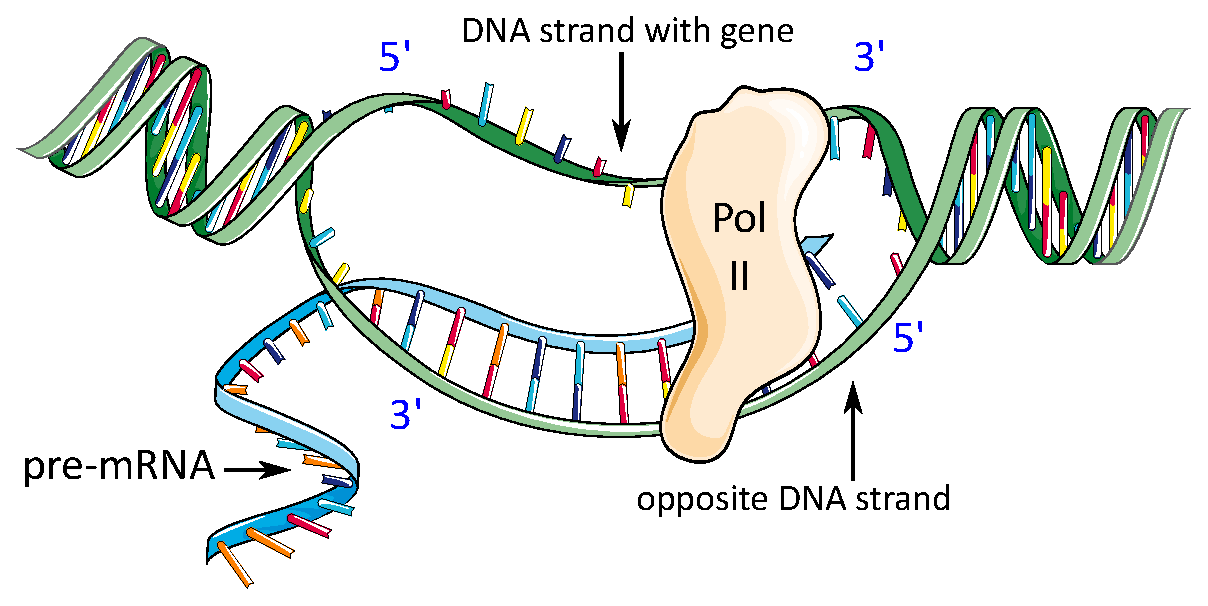
\includegraphics[width=0.75\textwidth,keepaspectratio]{images/intro/transcription}
    \caption[Illustration of DNA transcription.]{Illustration of DNA transcription by RNA Pol II to produce pre-mRNA\@. Image is adapted and altered from ``Transcription'' and ``Protein'' by Les Laboratoires Servier, licensed under CC BY 3.0 (\url{https://creativecommons.org/licenses/by/3.0/}).}
    \label{fig:intro:transcription}
\end{figure}
For coding genes, the first step in production of a peptide from a given gene is \textbf{transcription}, the production of RNA from a DNA sequence \cite{sainsbury2015}. RNA is a highly similar molecule to DNA, with the addition of a hydroxyl group to the 2' position of the pentose ring, and substitution of uracil (U) for thymine \cite{horton19_2006}. Transcription begins with recruitment of the RNA polymerase II (Pol II) enzyme by transcription factor proteins to a Transcription Start Site (TSS) region of a gene \cite{kapranov2009}. Pol II then reads a gene in the 5' to 3' direction (gene can be on either positive or negative strand), and synthesizes a fragment of RNA that is complementary to the opposite DNA strand (Figure~\ref{fig:intro:transcription}). This fragment is termed \textbf{pre-messenger RNA}, or pre-mRNA.

\begin{figure}[htb]
    \centering
    \includegraphics[width=0.6\textwidth,keepaspectratio]{images/intro/Chromosome-DNA-gene}
    \caption[High-level organization of DNA.]{High-level organization of DNA\@. DNA strands are wrapped around histone protein complexes to form nucleosomes, and entire DNA strands are termed chromosomes. DNA sequence contains genes (a feature of sequence information rather than a biochemical difference from intragenic DNA), which in turn contain introns, exons and various regulatory regions. ``Chromosome-DNA-gene'' by Thomas Splettstoesser is licensed under CC BY-SA 4.0 (\url{https://creativecommons.org/licenses/by-sa/4.0/}).}
    \label{fig:intro:dna_hierarchy}
\end{figure}
Genes contain functional regions termed \textbf{exons} and \textbf{introns} (Figure~\ref{fig:intro:dna_hierarchy}), demarcated by splice site sequences \cite{jo2015}. Exons contain instructions for sequences of amino acids to build peptides. Introns do not, but may serve regulatory and other functions. The next step in peptide production is splicing, in which a collection of proteins and functional RNA molecules termed the spliceosome excises introns from the pre-mRNA fragment \cite{will2011}. After addition of a 5' altered guanine cap \cite{shatkin1976} and a 3' poly-adenine tail \cite{guhaniyogi2001}, the new messenger RNA molecule is exported from the nucleus to the cytoplasm. By varying the exons that are included, one gene is able to produce multiple different mRNA molecules termed transcripts, each of which codes for a different peptide.

The mRNA is then processed by the ribosome, which assembles a peptide sequence based on the mRNA sequence \cite{horton19_2006}. This is termed \textbf{translation}. Three-letter sequences, termed \textbf{codons}, specify particular amino acids to be included in the peptide \cite{nirenberg2004}. Three of the 64 codons (UAA, UAG, UGA), termed stop codons, signal the ribosome to cease addition of amino acids and release the produced peptide. Ribosomes provide a scaffold for amino acid-bearing transfer RNA (tRNA) molecules complementary to each codon, and catalyze peptide bonds between newly arriving amino acids and the growing polypeptide chain \cite{steitz2008}. Peptides may undergo an enormous variety of additional post-translational modifications and other processing to produce mature and properly folded proteins \cite{conibear2020}.

Non-coding RNAs are also transcribed from the genome (potentially by different RNA polymerases \cite{turowski2016}) and may undergo splicing \cite{krchnakova2018} along with various other mechanisms of post-transcriptional modification \cite{leighton2018}. However these RNA molecules are not translated into peptides, rather they perform biological functions of their own. Also unlike mRNA, ncRNA is not always exported into the cytoplasm as some ncRNAs fulfill functions in the nucleus. Several classes of ncRNAs exist, such as micro RNAs (miRNA) which typically target complementary mRNA sequences for degradation to reduce expression of these genes, the aforementioned tRNAs essential to mRNA translation, ribosomal RNA (rRNA) which contributes to the ribosome structure, and long non-coding RNAs (lncRNA) which serve a variety of functions \cite{slack2019}.

Many DNA regions have regulatory functions instead of or in addition to serving as a template for RNA production. Critical to cell function, growth, and differentiation is \textbf{gene regulation}, or the ability of the cell to control the quantity of each protein it is capable of producing \cite{guo2014}. The relative amount of a gene or transcript's transcription is known as its expression. Cells of different types must express different genes to perform their various functions, and cells must alter expression in response to environmental or other stimuli. This is facilitated by the instability of mRNA in the cytoplasm (half-life highly variable but median \textapprox{}10~hours) \cite{yang2003}, therefore cells must continuously produce mRNA to maintain high expression, which grants them the ability to quickly reduce gene expression on demand. Increased expression is termed upregulation, and decreased expression downregulation.

A variety of mechanisms to regulate transcription are known, with three of the most important being DNA methylation, histone modification, and transcription factors. Methylation of the 5' position of cytosine to form 5-methylcytosine, particularly at cytosines followed by guanine (CpG), is known to repress transcription \cite{jin2011}. Histone proteins electrostatically adhere to DNA due to their positive charge. This interaction can be altered by modifying exposed histone residues along with substitution of variant histone proteins \cite{greer2012,ernst2010,bonneville2012}. For instance, histone acetylation (adding a negatively-charged functional group) tends to increase gene expression by decreasing the histone positive charge \cite{eberharter2002}, facilitating access to DNA by RNA Pol II and other enzymes involved in transcription. \textbf{Transcription factors} constitute a large family of proteins which bind to DNA regions called enhancers and recruit other DNA-binding proteins and transcriptional enzymes \cite{spitz2012}. These various mechanisms of DNA regulation constitute an essential component of the fantastically complex system that is the human cell.

\subsection{Replication}
\label{ssec:intro:dna_replication}
It is insufficient for cells to merely use DNA as a blueprint; in order to divide and produce new cells, the cell must copy its entire genome with high fidelity. This occurs during the S (synthesis) phase of the cell cycle, and requires a complicated assortment of proteins known as the \textbf{replisome} \cite{bellelli2020}. Given this complexity, we will only briefly outline the major events of DNA replication.

\begin{figure}[htb]
    \centering
    \includegraphics[width=0.9\textwidth,keepaspectratio]{images/intro/0323_DNA_Replication_altered}
    \caption[High-level illustration of DNA replication.]{High-level illustration of DNA replication. ``DNA Replication'' \cite{betts2013} by OpenStax is licensed under CC BY 4.0 (\url{https://creativecommons.org/licenses/by/4.0/}), and has been modified to highlight the DNA region being replicated and alter labels.}
    \label{fig:intro:replication_schematic}
\end{figure}
A single replisome is able to assemble 50 nucleotides per second \cite{chali1_2014}, which by itself would take over two years to replicate the entire human genome. To facilitate replication in a reasonable time frame, multiple replisomes assemble at sites termed replication origins (ori)\footnote{Though DNA synthesis occurs during the S phase, oris were `licensed' during G\textsubscript{1}.} and replicate the genome in parallel \cite{bellelli2020}. At the beginning of the S phase, the CMG helicase complex ``unzips'' the DNA double helix beginning at an ori to create a replication fork, and replication protein A (RPA) binds to the exposed DNA single strands (Figure~\ref{fig:intro:replication_schematic}). RPA recruits a replisome on each strand, and both replisomes traverse the strand in the 3'\textrightarrow{}5' direction, \textit{i.e.}\ away from the ori in opposite directions. In the replisome, DNA polymerase $\alpha$ (POL$\alpha$) lays down a short primer sequence, which is extended by POL$\varepsilon$ to create a new DNA strand termed the leading strand (extending in the 5'\textrightarrow{}3' direction), complementary to the original DNA single strand being traversed. Such strand extension entails adding nucleotides one at a time through phosphate linkages from the 3' hydroxyl group of the preceding nucleotide to the 5' hydroxyl of the new nucleotide. Meanwhile, POL$\delta$ synthesizes short DNA fragments (called Okazaki fragments) in the other direction (towards the ori) \cite{langston2006}, 3'\textrightarrow{}5' traversing the opposite source strand. Okazaki fragments are ligated to create a continuous DNA strand, called the lagging strand. Replication continues until the replisome encounters another replisome (from another ori), and CMG is disassembled to permit new double helices to form. Each new double-stranded DNA molecule contains one original strand and one newly synthesized, complementary strand. The end result of this process is two identical copies of the original genome, which will be equally divided among daughter cells during the M phase of the cell cycle.

Of interest, the machinery of DNA replication can be exploited \textit{in vitro} to ``amplify'' (extensively copy) a DNA sequence in a process termed polymerase chain reaction, or PCR \cite{bartlett2003}. This process utilizes RNA primers complementary to sequences flanking the sequence of interest, along with a thermostable DNA polymerase (typically isolated from extremophile bacteria) and deoxynucleotide triphosphate molecules (dNTPs, which have a chain of 3 phosphate groups linked to the deoxyribose 5' hydroxyl group) \cite{green2018}. In each PCR cycle, the solution is heated to separate double-strand DNA fragments into single strands, and cooled to permit new primer binding and for DNA polymerase to synthesize new complementary strands. Through repeated cycles, this reaction can geometrically increase the number of identical (except for polymerase errors) DNA fragments. PCR is used extensively throughout molecular biology, including detection of DNA sequences through quantification of DNA yields at each cycle (termed quantitative PCR or qPCR), and generation of the relatively large quantities of DNA typically necessary for sequencing.

\subsection{Mutation}
\label{ssec:intro:mutation}
A variety of events and mechanisms can lead to changes in a DNA sequence, which are termed \textbf{mutations} \cite{lodish2000}. In healthy human cells, mutations have been estimated to occur at a rate of $6 \times 10^{-11}$ per base per cell division \cite{lynch2010}, or roughly an average of one mutation per every five cell divisions. Depending on a mutation's position and the bases affected, mutations can give rise to phenotypes (effects of a gene) ranging from nonexistent to catastrophic, or even in rare cases beneficial. The possibility of mutations is therefore a double-edged sword; necessary for evolution, yet creating the possibility of deleterious mutations that lead to genetic disorders including cancer \cite{loewe2010}.

The most common forms of mutation affect one or a few bases. A change of a single base is termed a \textbf{single nucleotide variant} (SNV) \cite{katsonis2014}. A change of a purine to another purine, or a pyrimidine to another pyrimidine, is termed a \textbf{transition}. A change of a purine to a pyrimidine, or vice versa, is a \textbf{transversion}. If in a coding region of the genome, it may be \textbf{synonymous} or \textbf{nonsynonymous}. As there are 64 possible three-letter codons for 20 amino acids, the genetic code contains redundancy. Therefore, some SNVs do not change the protein product and are termed synonymous or silent, however in rare cases even synonymous SNVs may have phenotypic effects \cite{zheng2014}. Nonsynonymous SNVs do change the protein product, and can be further subdivided into \textbf{missense} or \textbf{nonsense}. Missense mutations change one amino acid codon or stop codon into another amino acid. Nonsense mutations change an amino acid codon into a premature stop codon, typically leading to a truncated and nonfunctional protein product \cite{jopling2014}. Insertions and deletions of bases can also happen, collectively termed \textbf{indels} for changes \textless{}~1000~bp \cite{sehn2015}. In coding regions, these can be classified as \textbf{frameshift} or \textbf{non-frameshift} indels. As translation occurs three letters of DNA at a time (the choice of first, second, and third bases termed the frame), addition or removal of a non-multiple of 3 bases disrupts translation of all downstream amino acids, usually with severe consequences for the protein. Non-frameshift indels affect multiples of 3 bases, therefore preserving the frame and downstream amino acids (unless a stop codon is inserted).

Cancers can possess a variable quantity of SNVs and indels, termed the \textbf{tumor mutation burden} (TMB) \cite{merino2020}. TMB is typically quantified as the number of detected mutations divided by the panel size in megabases. Though there is currently not a universal standard for TMB classification, tumors with TMB $\ge 10$ are often considered ``hypermutated'' or TMB-high (TMB-H) \cite{shao2020,keytrudafda2017}, with other tumors classified as TMB-low. Hypermutation is known to occur through a variety of mechanisms \cite{campbell2017}.

\begin{figure}[htb]
    \centering
    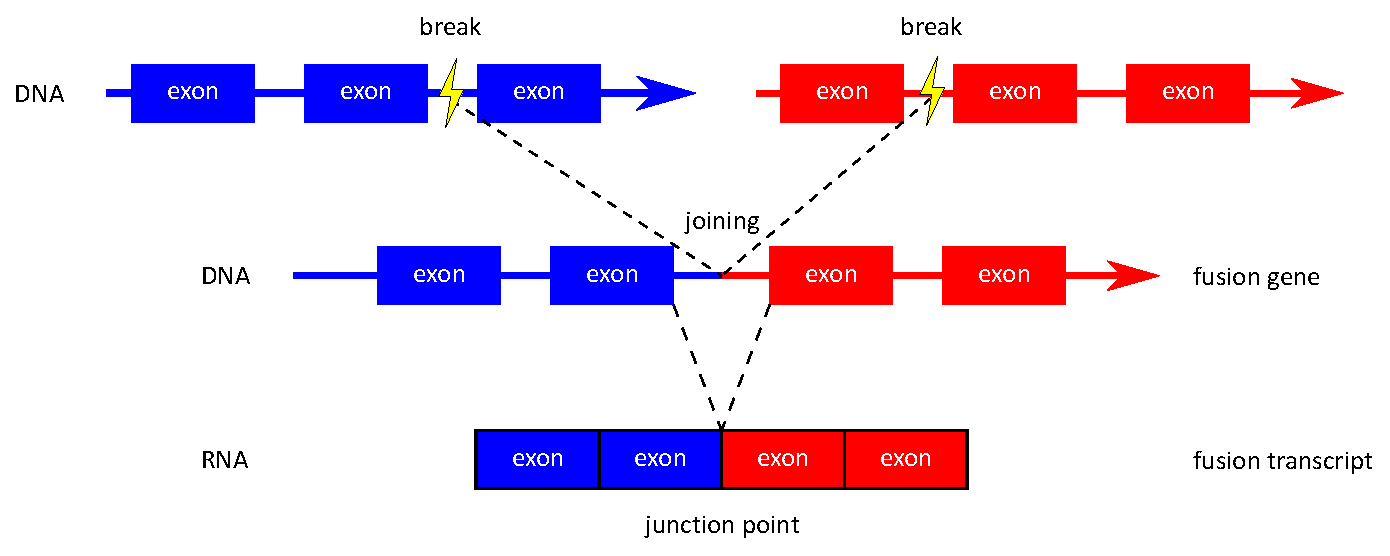
\includegraphics[width=0.9\textwidth,keepaspectratio]{images/intro/fusion_example}
    \caption[Illustration of a gene fusion.]{Illustration of a gene fusion. Double-strand breakage of at least one site creates free-floating fragments of DNA, which may rejoin new locations of chromosomes (either another breakage site as depicted here, or a chromosome end). If this occurs between coding genes, a new fusion gene is produced containing sequence from both partner genes. This may include exons and introns, giving rise to new fusion transcripts.}
    \label{fig:intro:fusion_schematic}
\end{figure}
Mutations can also affect larger DNA regions, up to and including entire chromosomes \cite{hastings2009}. Large DNA regions ($\ge 1000$~bp) can be gained or lost, a phenomenon termed \textbf{copy number variation} (CNV)\@. Copy number gains increase the number of copies of affected genes, which in term increases their expression as more mRNA can be synthesized in parallel. Loss of one copy of a gene can reduce its expression, and losing both copies (or a singular copy on a sex chromosome in a male) deletes the gene entirely from the cell. Another type of large DNA alteration is \textbf{rearrangement}, in which DNA strands are broken and recombine in new ways to form altered chromosomes \cite{hasty2014}. When breakpoints occur within or near genes, rearrangements can give rise to \textbf{gene fusions} \cite{rabbitts1994,osborne2007}, or new genes containing components of what were originally two (or rarely more) separate genes (Figure~\ref{fig:intro:fusion_schematic}). Such fusion genes may exert different effects than either of the original partner genes.

A wide variety of mechanisms for DNA mutation are known \cite{chakarov2014}. Mutational mechanisms can be divided into \textbf{exogenous mechanisms}, which originate outside the cell, and \textbf{endogenous mechanisms}, originating within the cell. Exogenous mechanisms include chemical agents termed \textbf{mutagens} \cite{benigni2011}, as well as environmental stressors such as ultraviolet light \cite{pfeifer2005} and ionizing radiation \cite{little2000}. Many endogenous mechanisms are known, therefore we will only describe some major mutational mechanisms (exogenous and endogenous) which are referenced in later chapters.

Tobacco smoke is well-known to be associated with cancer \cite{obe1984}, and contains multiple mutagens. Of particular interest are polycyclic aromatic hydrocarbons, especially benzopyrene \cite{demarini2004}. Benzopyrene is converted into an epoxide derivative by cytochrome P450 (CYP) family enzymes, and in turn binds to guanine in DNA \cite{iarc2012}. These large chemical groups disrupt the normal DNA double helix structure, producing a variety of SNVs, indels, and DNA breaks which lead to rearrangements \cite{cosmic_ms}. Many chemotherapeutic agents used to treat cancer are in fact mutagens, exploiting the increased sensitivity of dividing cells to disruption of DNA synthesis \cite{ferguson1996}. For instance, molecules of platinum-based agents (\textit{e.g.}\ cisplatin, carboplatin, oxaliplatin) can bind to multiple DNA bases, cross-linking DNA strands and interfering with DNA function and replication \cite{chen2013}, which introduces characteristic patterns of mutations \cite{pich2019}. Other agents such as gemcitabine and 5\nobreakdash-fluorouracil mimic building blocks of DNA\@. Gemcitabine masquerades as cytosine and is inserted into DNA, causing DNA polymerase to stall and truncating DNA strands. 5\nobreakdash-fluorouracil mimics uracil and blocks thymine synthesis, both preventing new DNA production during cell division and inducing T\textgreater{}G transversions \cite{christensen2019}.

Ultraviolet radiation (UV) is able to directly affect nucleotides. UVA (320--400~nm) oxidizes other cellular molecules to create oxygen free radicals, which react with guanine in particular to form 8-oxoguanine \cite{kielbassa1997}. UVB (280--320~nm) and UVC (200--280~nm) attack adjacent pyrimidine bases (\textit{e.g.}\ \texttt{CC} or \texttt{CT} sequences) in a cyclization reaction (occurring at their 5-6 position double bond) which cross-links the bases. Ionizing radiation directly attacks DNA causing double-strand breaks, and also creates DNA-damaging oxygen free radicals \cite{santivasi2014}. In addition, cytosine and 5-methylcytosine are prone to spontaneously deaminate to uracil and thymine respectively (conversion of 4 position amine group to carbonyl), which causes C\textgreater{}T transitions \cite{lewis2016}. Such mutations produce a characteristic age-associated pattern termed ``clock-like'' mutation \cite{alexandrov2015}.

\begin{figure}[htb]
    \centering
    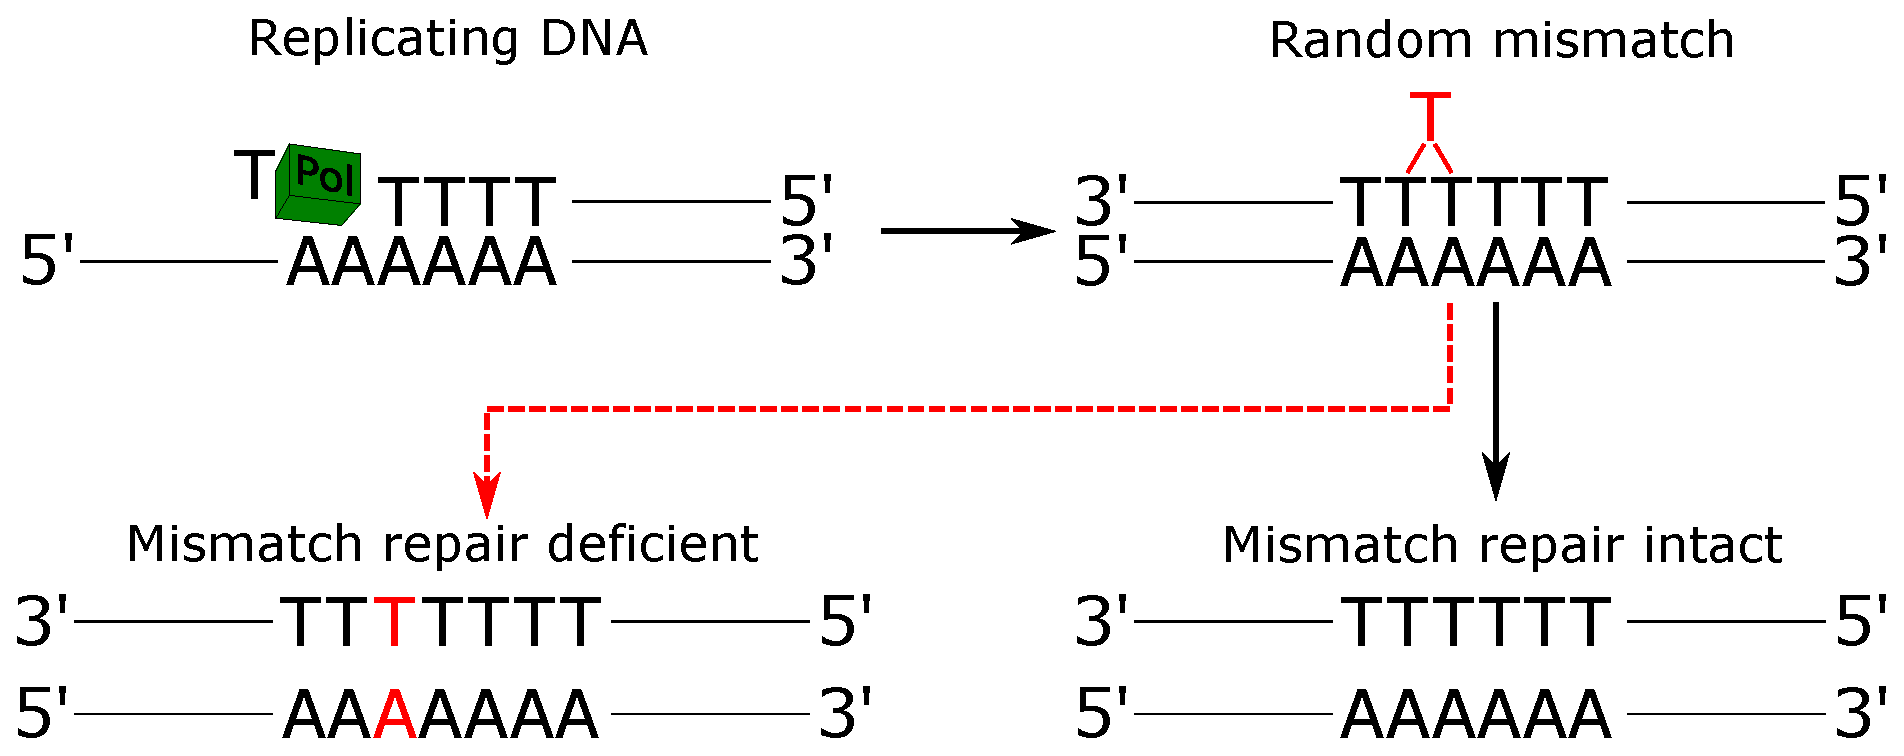
\includegraphics[width=0.9\textwidth,keepaspectratio]{images/intro/msi_schematic}
    \caption[Mechanism of microsatellite instability.]{Mechanism of microsatellite instability. Microsatellites are highly repetitive sequences which are prone to slippage during DNA replication. Failure of the mismatch repair system to repair such slippage results in random changes in the microsatellite sequence length. Reprinted by permission from Springer Nature: Springer, Detection of Microsatellite Instability Biomarkers via Next-Generation Sequencing, by Bonneville R, Krook MA, Chen HZ, Smith AM, Samorodnitsky E, Wing MR, Reeser JW, Roychowdhury S\@. \textcopyright{} 2020. \url{https://link.springer.com/protocol/10.1007\%2F978-1-4939-9773-2_5}.}
    \label{fig:intro:msi_schematic}
\end{figure}
Another mutational mechanism important in cancer is \textbf{microsatellite instability} (MSI). Microsatellites are short stretches of DNA composed of repeats of a 1--6~bp sequence (termed a motif) \cite{kelkar2010}. During DNA replication, a new strand of DNA that is slightly offset from the original sequence will still possess a high degree of complementarity, as most of the repetitive bases will still match \cite{levinson1987}. This permits DNA polymerases to ``slip'' (Figure~\ref{fig:intro:msi_schematic}), inserting or deleting copies of the motif and generating indel mutations (most microsatellites have 1~bp motifs) \cite{schloetterer1992}. MSI is one source of hypermutation, and will be discussed in further detail in Chapters \ref{ch:msilandscape} and \ref{ch:msiclones}. In addition, cells have evolved the \textbf{APOBEC} (Apolipoprotein B mRNA Editing Catalytic Polypeptide-like) family of nucleic acid editing proteins, \textit{i.e.}\ proteins with the primary (and counter-intuitive) function of \emph{inducing} mutations \cite{salter2016}. Some APOBEC members target DNA, either to facilitate somatic hypermutation in B cells\footnote{Recently, this has been disputed in favor of a reverse transcriptase-based mechanism \cite{steele2016}.} necessary to increase the variety of antibodies produced, or to scramble viral DNA.

\subsection{Repair}
%add stuff like Lynch syndrome here
With the many opportunities for mutation afforded by exogenous and endogenous mechanisms, the human cell is able to suppress mutations such that a single zygote can give rise to the \textapprox{}$3.7 \times 10^{13}$ cells in the average adult human body without incident \cite{bianconi2013}. This occurs by a variety of \textbf{repair mechanisms} \cite{chatterjee2017}, a few of which will be outlined here. Additionally, the cell has failsafe mechanisms that allow a cell to essentially self-destruct (termed \textbf{apoptosis}) if mutations are irreparable.

DNA repair begins with the polymerases during DNA replication, most of which (including POL$\varepsilon$ and POL$\delta$) have \textbf{proofreading} capabilities \cite{albertson2006}. This typically consists of a 3'\textrightarrow{}5' exonuclease domain, which removes newly added bases in response to incorrect nucleotide pairing with the original strand \cite{bebenek2018}. Other, non-polymerase exonucleases assist in proofreading \cite{mason2012}. Proofreading reduces the polymerase error rate by a hundred to a thousand-fold. Of note, some cancers acquire mutations in the proofreading domain of POL$\varepsilon$, leading to acquisition of substantial hypermutation \cite{schlesner2015}. POL$\varepsilon$-mutant cancers are often ultra-hypermutated (TMB $\ge 100$ muts/Mb) \cite{campbell2017}.

Also serving to correct replication errors is the \textbf{mismatch repair} (MMR) system, which detects and corrects DNA polymerase slippage \cite{baretti2018} (Figure~\ref{fig:intro:msi_schematic}). This system consists primarily of the MLH1/MSH2 and MSH6/PMS2 heterodimers, and also involves several additional proteins within the MSH and MLH families \cite{fishel2015}. It is believed that MSH proteins traverse newly synthesized DNA to ``scan'' it for the increased molecular flexibility which indicates a mismatch (due to its weaker affinity for the correct base's complement). Upon encountering a mismatch, more MSH protein copies are recruited to the site, followed by other proteins (including MLH family proteins) which excise a region of the new DNA strand around the mismatch. The single-strand gap is then filled in by a DNA polymerase.

Most important to repair of DNA damage is \textbf{base excision repair} (BER) \cite{zharkov2008}. Briefly, a family of 11 DNA glycosylases is responsible for patrolling DNA to identify various lesions, including but not limited to alkylated and oxidized bases \cite{krokan2013}. Although differing in details, when encountering a lesion the DNA glycosylase excises the damaged base, the deoxyribose is removed by either APE1 or POL$\beta$, and $POL\beta$ replaces the nucleotide \cite{wallace2014}. BER is also important for repair of single-strand DNA breaks. These are detected by the PARP1 and PARP2 proteins, which recruit BER enzymes including XRCC1 to trim damaged bases at the break ends and facilitate reconstitution of the strand.

BER is limited in that it can only recognize a fixed subset of DNA damage mechanisms. The \textbf{nucleotide excision repair} (NER) pathway provides a more general means of DNA sequence repair, capable of recognizing DNA lesions which distort the double helix \cite{spivak2015}. NER is also capable of detecting some forms of damage that affect multiple bases, for instance UV-induced pyrimidine dimerization. NER begins through either the transcription-coupled repair or the global genomic repair sequence. In transcription-coupled repair, DNA lesions which block RNA Pol II progression cause the polymerase to dissociate from DNA and recruit NER enzymes including TFIIH\@. In global genomic repair, double helix distortions are recognized by the XPC-hRAD23b-CETN2 complex (possibly with the help of the XPE-DDB1 complex), which recruits TFIIH\@. Other XP family proteins proceed with the repair. First, \textapprox{}30~bp around the lesion are unwound. Next, the intact DNA on the complementary strand is protected by RPA and the damaged section is excised. Finally, the gap is filled by a DNA polymerase \cite{marteijn2014}.

Cells also possess two mechanisms of double-stranded break (DSB) repair; \textbf{homologous recombination} (HR) and \textbf{non-homologous end joining} (NHEJ) \cite{mladenov2016}. HR depends on the presence of a second genome copy, therefore can only function after the S phase \cite{li2019_hr}. In this pathway, DSB are recognized by the MRN protein complex (consisting of MRE11, RAD50 and NBS1), which then trims the break ends to produce single-strand overhangs. These overhangs then invade the intact genome and DNA polymerases reconstruct the original sequence across the breakpoint using the intact genome as a reference. In contrast, NHEJ can function throughout the cell cycle, however without a second genome copy it cannot faithfully recover the sequence at the breakpoint which leads to random mutations\footnote{The relative accuracy of HR and NHEJ has been disputed, with findings of high HR error rates \cite{rodgers2015} and accurate NHEJ \cite{betermier2014}.} \cite{davis2013}. In this pathway, DSB are recognized by the Ku70/Ku80 heterodimer, which binds to both break ends to stabilize the site. Ku70/Ku80 recruits a variety of proteins, including TdT (terminal deoxynucleotidyl transferase) which adds random nucleotides to a DNA fragment \cite{boubakour2012}, and POL$\lambda$ which is capable of synthesizing short DNA fragments without a template (and hence unlikely to match the former sequence) \cite{ramadan2004}. After the break ends have been appropriately prepared, they are ligated by DNA ligase IV and Ku70/Ku80 is ubiquitinylated and degraded.

Despite these and other DNA repair mechanisms, not all mutations can be adequately repaired. Most mutations are of little to no consequence \cite{nei2010}, for instance mutations affecting intragenic regions (the stretches of DNA in between genes) or silent mutations and which do not happen to be in a region important for gene regulation. However, given the risk of mutations inducing cancer, cells have mechanisms to induce apoptosis should DNA repair fail or in the case of overwhelming DNA damage. One such mechanism involves the protein \textbf{p53} \cite{schlereth2010}, encoded by the gene \textit{TP53}. This protein is involved in multiple repair pathways including BER, NER and DSB repair \cite{offer2002}. Upon detection of DNA damage, p53 binds to p21, and p21 inhibits the cyclin~E/Cdk2 and cyclin~D/Cdk4 complexes to cause G\textsubscript{1} cell cycle arrest, along with downregulation of cdc25C expression to arrest a cell at G\textsubscript{2}/M \cite{chen2016}. If p53 remains activated for a sufficient time (because DNA repair has not concluded), it upregulates pro-apoptotic proteins such as the BH3-only protein family which attacks the mitochondrial outer membrane, leading to a cascade of events culminating in death of the cell.

\section{Overview of genomics}
\label{sec:intro:genomics}
Realization of the central role of DNA in the composition and function of an organism has led to the field of \textbf{genomics}, or study of genomes \cite{delgiacco2012}. As we have seen, genomes carry information in their sequence of nucleotides (Section~\ref{ssec:intro:dna_function}). Therefore, at the core of genomics is DNA sequencing, or the elucidation of DNA sequence \cite{weissenbach2016}. In turn, the ever-increasing quantities of data generated by sequencing methodologies has spurred developments in \textbf{bioinformatics}, the computational study of biological data. Genomics has yielded substantial insights with clinical relevance, especially in oncology \cite{shendure2019}.

\subsection{Beginnings}
\label{ssec:intro:seq_beginnings}
\begin{figure}[htb]
    \centering
    \includegraphics[width=0.9\textwidth,keepaspectratio]{images/intro/sanger_sequencing}
    \caption[High-level illustration of Sanger sequencing.]{High-level illustration of Sanger sequencing. Dideoxynucleotide triphosphate (ddNTP) molecules induce random termination of complementary strand synthesis, producing a distribution of fragments of different lengths (left). These fragments are size-sorted by gel electrophoresis (center). The particular ddNTP is determined for each fragment size, and the reverse complement of the ddNTP sequence yields the original DNA sequence. Figure by Wen and Zhong \cite{wen2019} is licensed under CC BY-NC-SA 3.0 (\url{https://creativecommons.org/licenses/by-nc-sa/3.0/}).}
    \label{fig:intro:sanger_schematic}
\end{figure}
After early experiments in sequencing of short RNA fragments \cite{minjou1972}, Sanger \textit{et al} developed the first practical method of sequencing genes and larger regions \cite{sanger1977,sanger1978}. This method, today termed Sanger sequencing, makes use of dideoxynucleotides which lack 3' hydroxyl groups. In current practice, each of the four dideoxynucleotides is typically labeled with a different fluorophore. Similarly to a PCR experiment (Section~\ref{ssec:intro:dna_replication}), primers and a DNA polymerase are added to a solution containing the DNA of interest, however dideoxynucleotide triphosphate molecules (ddNTPs) are added as well as dNTPs. DNA polymerase stops after inclusion of a dideoxynucleotide due to its inability to accept a 3' phosphate linkage. Therefore, Sanger sequencing yields a collection of fragments of different lengths, including many incomplete fragments ending in a single dideoxynucleotide (Figure~\ref{fig:intro:sanger_schematic}). These fragments are then stratified by length via gel electrophoresis, and the attached fluorophore is read to determine the identity of the base at the position given by the fragment length. Although Sanger sequencing has today largely been supplanted by newer methods, it remains in use for small-scale sequencing and as a method for validating genetic findings revealed by other sequencing methods.

Since its discovery, Sanger sequencing was applied to increasingly larger genes and genomes \cite{shendure2017}. As sequencing increased in scale, interest grew in the prospect of sequencing an entire human genome, leading to the formation of the Human Genome Project in 1990 \cite{green2015}. Its goals were to produce an entire human genome sequence by 2005 with a total budget of \$3~billion \cite{sawicki1993}. This would entail so-called ``shotgun sequencing''; creating overlapping clones of short human genome fragments which would be Sanger sequenced. The fragments would then be computationally stitched together and localized to a human genome region based on ``anchor'' regions of previously known sequence and position. During the 1990s, several improvements were made to Sanger sequencing (particularly increased automation), however a computational breakthrough by Celera, Inc.\ reduced the need for anchor regions and led to the Project's completion in 2001 \cite{venter2001}, four years ahead of schedule and \$300~million under budget \cite{kling2005,gyles2008}.

\begin{figure}[htb]
    \centering
    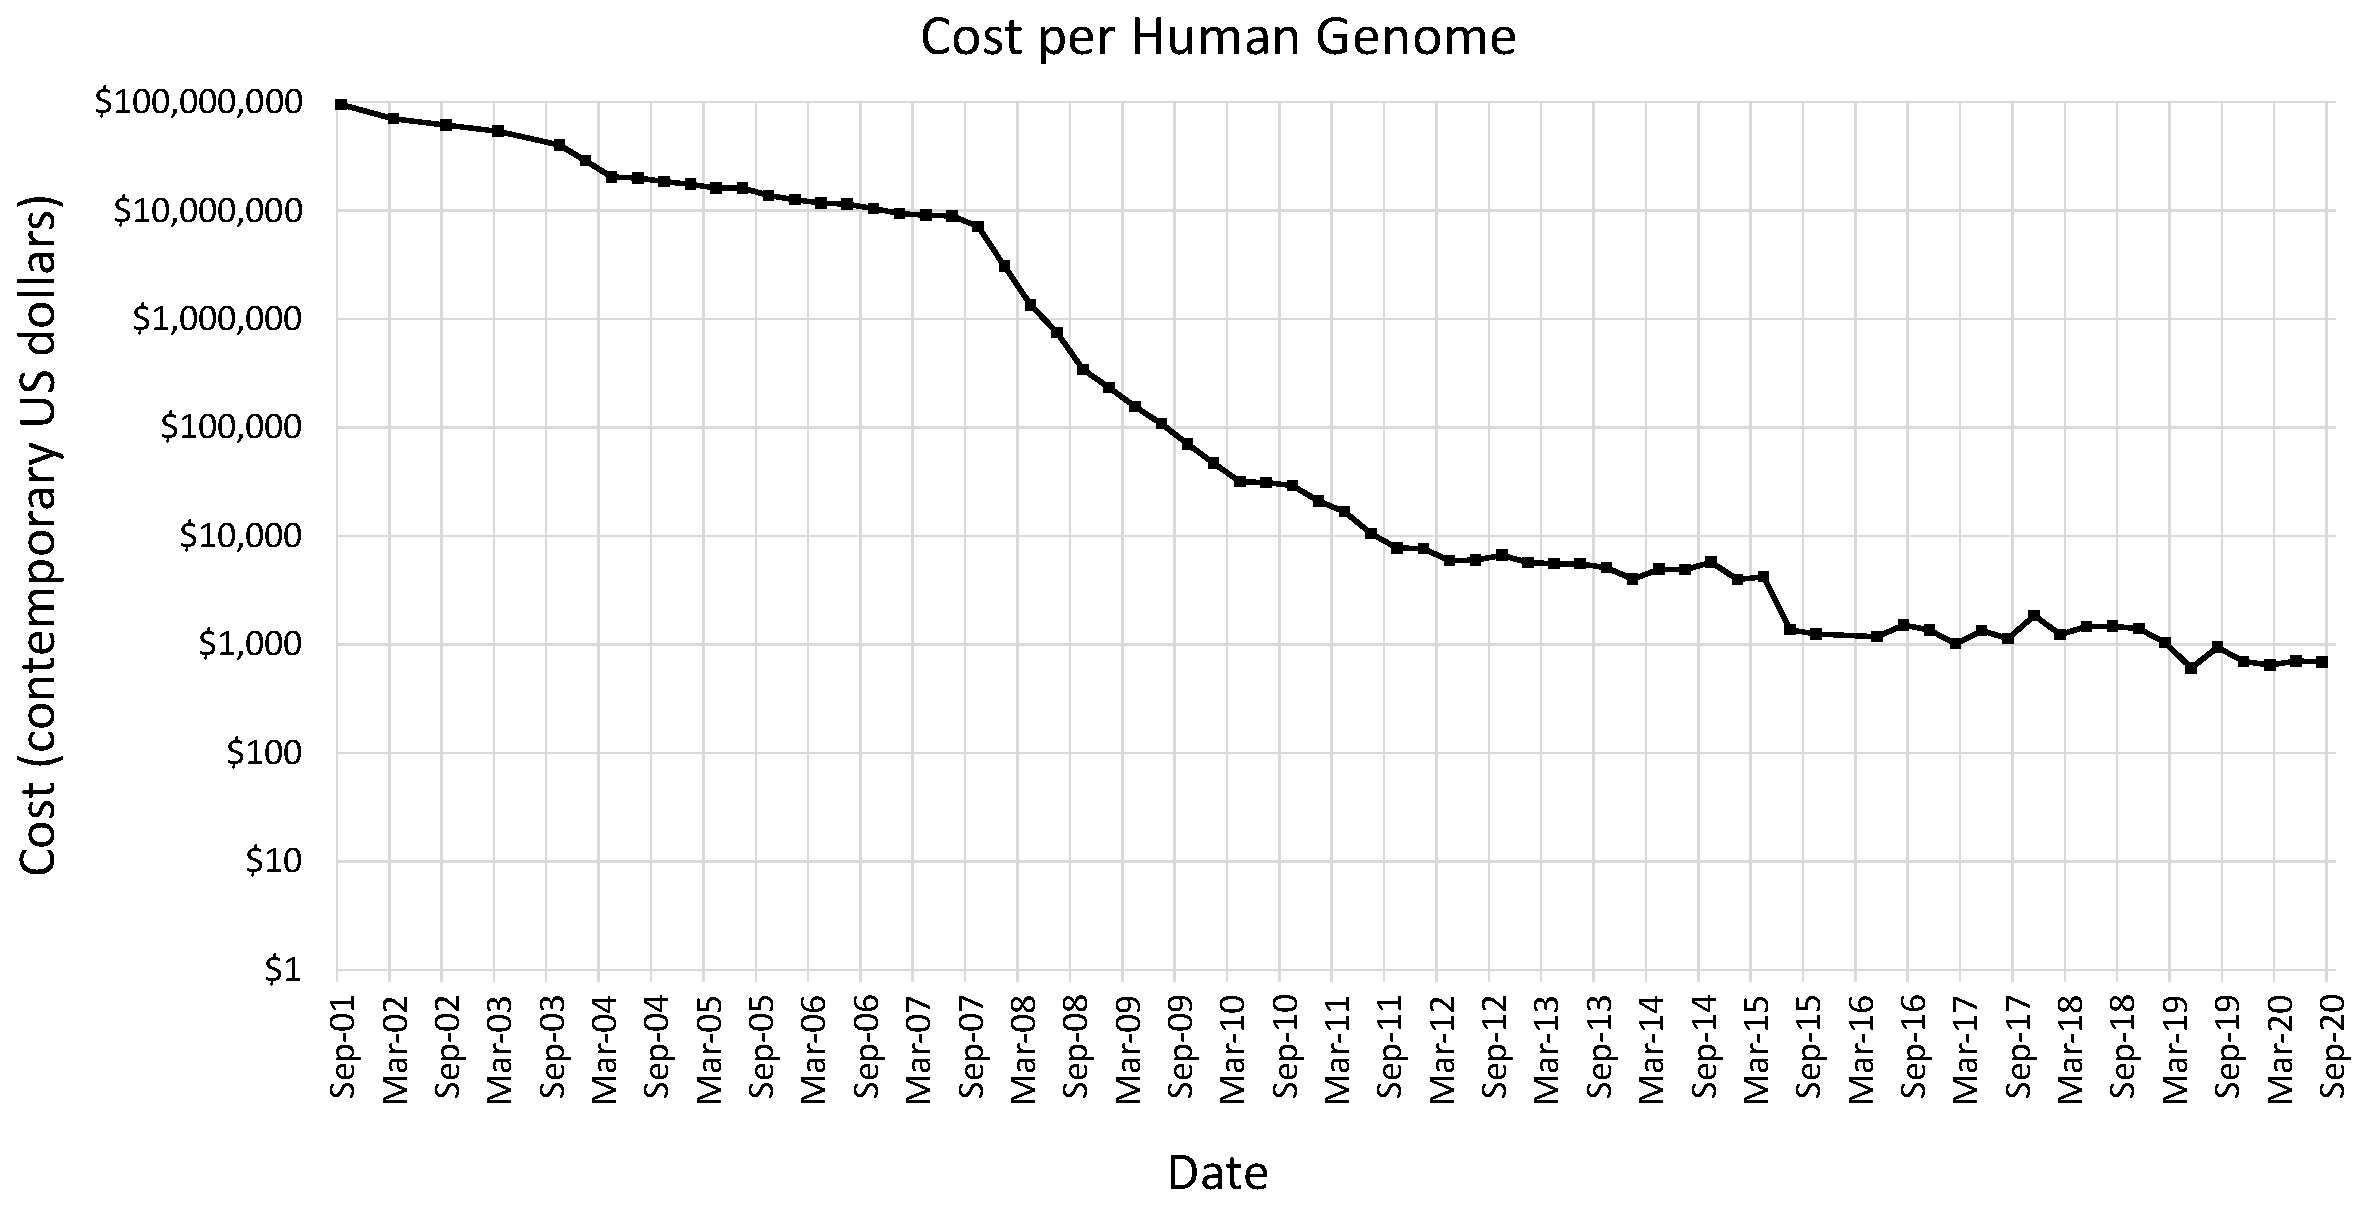
\includegraphics[width=0.95\textwidth,keepaspectratio]{images/intro/sequencing_cost}
    \caption[Cost of human genome sequencing from 2001--2020]{Cost of human genome sequencing from 2001 to 2020. The cost to sequence a single human genome (\textit{i.e.}\ 1\texttimes{} coverage) has declined logarithmically during the 21\textsuperscript{st} century, leading to massive growth in DNA sequencing experiments. Data obtained from the National Human Genome Research Institute (NHGRI) \cite{wetterstrand2020}.}
    \label{fig:intro:sequencing_cost}
\end{figure}
Breakthroughs in DNA sequencing have sharply accelerated in the 21\textsuperscript{st} century, such that the cost to sequence a human genome's worth of DNA has logarithmically decreased (Figure~\ref{fig:intro:sequencing_cost}). This has led to an explosion in sequencing-based science, which has been particularly impactful in cancer research by permitting cost-effective sequencing of patient tumor samples to identify genetic changes, and even facilitated clinical usage of DNA sequencing to guide cancer treatment, prognosis, and prediction \cite{rizzo2012}.

\subsection{Next-generation sequencing}
Central to this explosive growth in DNA sequencing (DNA-seq) has been next-generation sequencing, or NGS\@. Unlike Sanger sequencing, NGS is massively parallel, capable of simultaneous sequencing of millions of DNA fragments automatically \cite{wheeler2008}. This has rendered genome-scale experiments tractable for individual laboratories, and been instrumental in the precipitous decline of sequencing time and costs \cite{vandijk2014}. Additionally, the large quantities of data generated by NGS has made quantitative RNA sequencing (RNA-seq) possible, in which reverse transcriptase is used to generate complementary DNA (cDNA) fragments which are then sequenced \cite{wang2009}. RNA-seq permits high-throughput detection of relative gene expression along with detection of gene rearrangements. NGS can be single-end or paired-end. In single-end sequencing, a certain number of bases of one end of a DNA fragment is read, yielding one sequencing read per fragment. Paired-end sequencing reads bases on both ends of the fragment; though the intervening sequence might not be read the fragment ends remain associated, and two reads are obtained per fragment.

\begin{table}[H]
	\begin{center}
		\begin{tabular}{ccccc}
			& & \textbf{Max read} & \textbf{Max throughput} & \textbf{Error} \\
			\textbf{Platform} & \textbf{Chemistry} & \textbf{length (bp)} & \textbf{per run} & \textbf{rate} \\
			\hline
			\textbf{454} & SBS, pyrosequencing & 1000 & 700~Mb & 1\% \\
			\textbf{Illumina} & SBS, reversible terminators & 300 & 3~Tb & \textless{}1\% \\
			\textbf{SOLiD} & Ligation & 75 & 320~Gb & \textless{}0.1\% \\
			\textbf{Ion Torrent} & Semiconductor & 600 & 15~Gb & 1\%
		\end{tabular}
	\end{center}
	\vspace{-0.3cm}
	\caption[Comparison of major NGS platforms.]{Comparison of the four most popular next-generation sequencing platforms. Statistics for 454 and SOLiD sequencing are from 2016 \cite{goodwin2016}, and data for Illumina and Ion Torrent from 2020 \cite{kanzi2020}. Throughput is measured in base pairs sequenced. SBS: sequencing by synthesis.}
	\label{table:intro:ngs_platform_comparison}
\end{table}
Next-generation sequencing began in 2005 with the pyrosequencing method of sequencing by synthesis developed by 454 Life Sciences \cite{margulies2005}. In 2006, Solexa, Inc.\ (now part of Illumina, Inc.)\ released the Genome Analyzer, which pioneered the reversible terminator method of sequencing by synthesis most popular today \cite{bennett2004,bentley2008}. This was followed by SOLiD sequencing by ligation from Applied Biosciences, Inc.\ (ABI) in 2007 \cite{valouev2008}, and semiconductor sequencing by Ion Torrent in 2010 \cite{rothberg2011}. Each of these four major NGS platforms have advantages and disadvantages (Table~\ref{table:intro:ngs_platform_comparison}) \cite{goodwin2016,kanzi2020}, though here we will focus on the Illumina sequencing platform used in all of the studies we will present.

\begin{figure}[htb]
    \centering
    \begin{subfigure}{0.25\textwidth}
        \includegraphics[width=\linewidth,keepaspectratio]{images/intro/illumina_library_prep}
        \caption{}\label{fig:intro:library_prep}
    \end{subfigure}%
    \hfill%
    \begin{subfigure}{0.73\textwidth}
        \includegraphics[width=\linewidth,keepaspectratio]{images/intro/illumina_library_enrichment}
        \caption{}\label{fig:intro:library_enrichment}
    \end{subfigure}
	\vspace{-0.3cm}
    \caption[Library preparation for NGS.]{Library preparation and target enrichment for next-generation sequencing. (\subref{fig:intro:library_prep}) Genomic DNA is fragmented into short DNA fragments and adapter sequences are ligated to each end. This allows PCR amplification of these sequences with primers complementary to known adapter sequences. These adapters also contain sequences required by the sequencing instrument (for Illumina sequencing, complementary to oligonucleotides on the flow cell) along with a sample-specific sequence which permits multiplexing of multiple biological samples in the same sequencing run. (\subref{fig:intro:library_enrichment}) A sequencing library can be enriched for fragments derived from a desired region of the genome. This is frequently performed using a panel of biotinylated probes complementary to the regions of interest, enabling efficient separation of fragments binding to these probes using streptavidin-coated, metal beads. Source: Illumina, 2017, An Introduction to Next-Generation Sequencing Technology. Used under license from Illumina, Inc. All Rights Reserved.}
    \label{fig:intro:seq_library}
\end{figure}
The first step in Illumina sequencing is library preparation. DNA is extracted from the cells to be sequenced and fragmented (Figure~\ref{fig:intro:library_prep}), often by sonication which mechanically fragments DNA \cite{sambrook2006}. Next, adapter sequences are ligated. For Illumina sequencing, an adapter consists of a constant region termed P5 or P7 (P5 and P7 adapters both necessary in a sequencing run), an index region, and a sequencing primer binding site. To generate the tens to hundreds of nanograms of DNA often necessary for sequencing \cite{aigrain2016}, the DNA is amplified by PCR using primers complementary to the P5/P7 sequences.

Researchers and clinicians are frequently interested in subsets of a genome. For instance, a cancer-focused study or clinical assay may focus on cancer-associated genes such as tumor suppressors and DNA repair genes. In whole exome sequencing, the exons of all known protein-coding genes (collectively termed the exome) are desired \cite{choi2009}. This is achieved by a collection of oligonucleotides (termed a panel) bearing complementary sequence to the desired genome regions and linked to biotin molecules (Figure~\ref{fig:intro:library_enrichment}). The panel is allowed to bind to the library, a process termed hybridization. Streptavidin-coated metal beads are introduced into the solution which strongly bind the hybridized fragments. The beads are extracted by magnetic separation, retaining the fragments of interest (``on-target'') to the exclusion of other DNA fragments (``off-target'').

\begin{figure}[htb]
    \centering
    \hspace{0.5cm}%
    \begin{subfigure}{0.45\textwidth}
        \includegraphics[width=\linewidth,keepaspectratio]{images/intro/illumina_seq_cluster}
        \caption{}\label{fig:intro:illumina_seq_cluster}
    \end{subfigure}%
    \hfill%
    \begin{subfigure}{0.45\textwidth}
        \includegraphics[width=\linewidth,keepaspectratio]{images/intro/illumina_seq_seq}
        \caption{}\label{fig:intro:illumina_seq_seq}
    \end{subfigure}%
    \hspace{0.5cm}
	\vspace{-0.3cm}
    \caption[Overview of Illumina sequencing by synthesis.]{Overview of Illumina sequencing by synthesis. (\subref{fig:intro:illumina_seq_cluster}) To permit sequencing, input DNA fragments must be separated and amplified. This is accomplished by binding of DNA to flow cell oligonucleotides followed by bridge amplification, resulting in multiple clusters of fragments with identical sequence. (\subref{fig:intro:illumina_seq_seq}) The actual sequencing begins with single-stranded DNA clusters adhered to the flow cell, and occurs through multiple cycles by gradually synthesizing a complementary strand. In each cycle, fluorophore-labeled reversible terminators are introduced to extend the new strand by one base, the flow cell is imaged to read the fluorescence signals, and the nucleotide protecting groups are cleaved. Source: Illumina, 2017, An Introduction to Next-Generation Sequencing Technology. Used under license from Illumina, Inc. All Rights Reserved.}
    \label{fig:intro:illumina_seq}
\end{figure}
The DNA is then introduced to the flow cell, a glass substrate coated with two oligonucleoties; one complementary to the P7 adapter sequence, and the other with the P5 sequence. The DNA strands in the library bind to the flow cell (Figure~\ref{fig:intro:illumina_seq_cluster}). The flow cell-bound oligonucleotide is extended by a DNA polymerase to create an entire complementary DNA fragment tethered to the flow cell. Its free end is complementary to the P5 sequence, and binds to a nearby P5 oligonucleotide to create a bridge. The P5 oligonucleotide is extended by DNA polymerase, and the strands again separate. Repeated cycles of this process, termed ``bridge amplification'', creates multiple copies of each flow cell-bound input DNA fragment in the same region (or ``cluster'') of the flow cell \cite{buermans2014}.

The library is now ready for DNA-seq. A solution of modified nucleotides with 3' protecting groups (termed ``reversible terminators'') and fluorophores is added, and the DNA polymerase is able to incorporate one nucleotide  (Figure~\ref{fig:intro:illumina_seq_seq}). The entire flow cell is imaged by a high-resolution camera, yielding a pattern of colored dots in which each dot (corresponding to a cluster) represents a base added to a DNA fragment. In this way, each machine cycle is able to determine a base of millions of fragments at once. After imaging, the protecting groups are removed and new fluorophore-labeled reversible terminators introduced to begin the next cycle. This process repeats for multiple cycles (often 300), generating millions to billions of reads. A flow cell may be divided into ``lanes'' (depending on the specific sequencing instrument), permitting multiple simultaneous NGS experiments per machine run.

\subsection{Emerging sequencing technologies}
DNA-seq techniques and technology remain an active area of research and commercial interest. One notable advance in library preparation is single-cell sequencing \cite{navin2011}. These protocols are capable of uniquely barcoding genomes, genomic regions, or even mRNA molecules from individual cells to permit detailed genomic maps of cell to cell variability. Another innovation in sequencing libraries is the use of UMIs (Unique Molecular Identifiers) \cite{kivioja2012}. The original DNA or RNA sample contains genetic material from multiple cells (except in single-cell experiments). However, the necessary library amplification step also creates duplicate fragments, therefore it is typically impossible to distinguish duplicate fragments derived from different pieces of original DNA from fragments artificially duplicated by PCR or from a single cluster misread as multiple clusters by the imager (optical duplicates). UMIs solve this problem by including short random sequences in different adapter molecules which are later sequenced. This permits computational differentiation between PCR\slash{}optical duplicates and true duplicate original fragments, enhancing the quantitative accuracy of determining the relative abundance of genomic regions which is particularly important for RNA-seq and CNV calling. Technical duplicates can in fact be leveraged through ``consensus calling'', in which multiple reads from the same original fragment are compared to increase confidence in the fragment sequence.

Multiple new sequencing methods have been developed in recent years, collectively termed ``third-generation'' sequencing \cite{vandijk2018}. Leading third-generation methods include PacBio sequencing and Oxford Nanopore. PacBio sequencing (commercialized in 2011) circularizes input DNA fragments and employs a fluorescence-based sequencing by synthesis approach \cite{eid2009}. The circularization step permits each individual fragment to be sequenced multiple times, increasing sequencing accuracy with each revolution of the DNA fragment through the polymerase. Nanopore sequencing (released in 2014) utilizes an entirely different approach; DNA fragments are fed through a membrane containing protein nanopores, and the differing electrical charges of nucleotides are read as each fragment traverses a nanopore \cite{jain2015}. Though these methods have yet to displace Illumina sequencing, they are continuing to mature and have the distinct advantage of generating much longer read lengths (on the order of tens of kilobases) than any NGS platform.

\subsection{Basics of computational analysis}
The end result of next-generation sequencing is a collection of DNA fragments and associated quality scores\footnote{This may require a demultiplexing step which is typically performed by the sequencing instrument.}. These are typically stored in FASTQ format, which for each read contains its assigned name (important for tracking read pairs from paired-end sequencing, and encoding the flow cell position to reduce optical duplicates), the DNA sequence in ASCII-encoded plaintext, and quality scores in Phred format. Phred scores \cite{ewing1998} encode the probability of an incorrect base call as follows:
\begin{equation}
     Q = -10\log_{10}(P_{\text{error}})
\end{equation}

\begin{figure}[htb]
    \centering
    \begin{subfigure}{0.55\textwidth}
        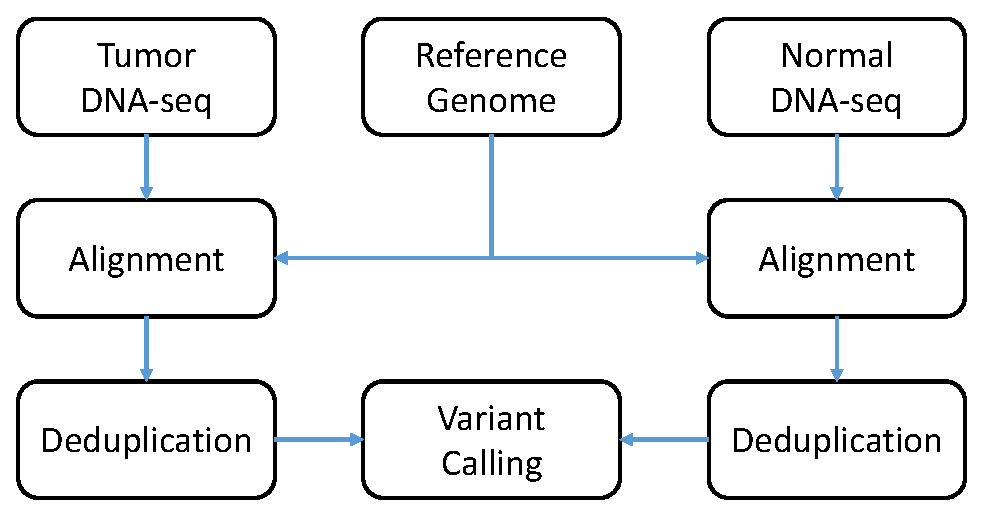
\includegraphics[width=\linewidth,keepaspectratio]{images/intro/info_flowchart_dna}
        \caption{}\label{fig:intro:info_flowchart_dna}
    \end{subfigure}%
    \hfill%
    \begin{subfigure}{0.35\textwidth}
        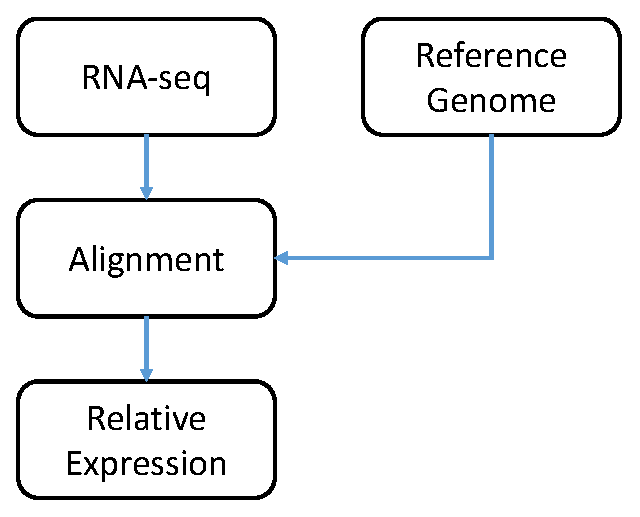
\includegraphics[width=\linewidth,keepaspectratio]{images/intro/info_flowchart_rna}
        \caption{}\label{fig:intro:info_flowchart_rna}
    \end{subfigure}
	\vspace{-0.3cm}
    \caption[Overview of common bioinformatics steps in DNA-seq and RNA-seq.]{Overview of common bioinformatics steps in DNA-seq and RNA-seq processing. (\subref{fig:intro:info_flowchart_dna}) Depicted here is a generic somatic variant calling workflow for cancer genomic analysis, where reads from tumor and normal DNA sequencing are aligned to a reference genome, duplicate reads removed, and somatic variant calling performed. (\subref{fig:intro:info_flowchart_rna}) In this generic RNA-seq experiment, RNA-seq reads are aligned to a reference genome and the relative coverage of exons, transcripts, and genes is computed.}
    \label{fig:intro:info_flowcharts}
\end{figure}
The first analysis step is typically alignment of sequences to the organism's reference genome (Figure~\ref{fig:intro:info_flowcharts}). In the case of humans, the first reference genomes were created by the Human Genome Project and Celera Inc.\ (Section~\ref{ssec:intro:seq_beginnings}). Today, standard reference genomes for human, mouse, rat, zebrafish, and chicken are curated by the Genome Reference Consortium, part of the NIH\@. A variety of software tools have been developed and remain in common use \cite{li2010}. Aligning short reads from NGS to a long reference genome is typically a two-step process. First, the entire genome must be searched for likely hits, for example utilizing hash tables \cite{altschul1990} or graph-based representations of the genome (\textit{e.g.}\ suffix trees \cite{abouelhoda2004}, Burrows-Wheeler transform \cite{burrows1994}). The second step entails semi-global alignment of the read with the sequence near each likely hit, which typically utilizes dynamic programming to achieve $O(mn)$ runtime such as the Needleman-Wunsch algorithm \cite{needleman1970} with zero initial and final gap penalties. Aligners typically output data in the BAM format\footnote{BAM is increasingly being supplanted by CRAM, which encodes the same information but with sequences represented as edits to the reference genome to reduce file sizes.} \cite{samtools}, a block GZIP-compressed representation of read sequences, quality scores, alignments and metadata.
%need to detail DP or alignment more?

After alignment, reads from DNA-seq (but not RNA-seq) must be deduplicated unless UMI-containing adapters were used, to remove optical and PCR duplicates. Typically aligned reads are sorted by position (requiring $O(n\log(n))$ time) and duplicates marked in one pass. Quality control metrics are typically computed, for instance the percent of reads which aligned to the genome or a genomic subset (if a capture panel was used), and the proportion of G/C bases in read sequence. A variety of other bioinformatics methods can be applied depending on experimental conditions and expected biases, for instance end-trimming of reads (as base quality scores typically decline with later sequencing cycles) \cite{martin2011} or normalization of quality scores \cite{mckenna10}.

An enormous variety of analyses have been developed utilizing aligned reads. For DNA, two common downstream analyses are variant calling and CNV calling. Typically variant calling identifies changes in read sequences from the reference genome and performs statistical calls to identify likely SNVs and indels \cite{pirooznia2014}. This can be performed with one sample alone to identify changes from a germline such as population-level SNPs, or with two samples (typically a tumor and matched normal DNA from the same patient) to identify somatic mutations. CNV calling compares the relative quantity of reads at different locations in the genome (the ``coverage'' of these locations) to a copy-neutral reference (usually either a matched normal or pooled panel of normals from multiple individuals) to detect relative gains and losses of genomic regions. A wide variety of tools are available today for variant and CNV calling, implemented using diverse methods of varying levels of sophistication. RNA-seq experiments are typically analyzed to quantify relative gene expression, a process superficially similar to CNV calling of DNA but with unique considerations due to varied splicing of genes \cite{conesa2016}. This can be performed within a single sample, in which expression is typically normalized for gene/transcript length, or between groups of samples in a differential expression experiment to identify genes upregulated or downregulated in one group versus another.

\section{Tumor heterogeneity}
Cancer in humans is an exceptionally complex disease. Considering cancer as a singular `disease' is a misnomer, as human cancer can be classified in a multitude of ways. For instance, cancer is frequently classified by organ site, such as lung cancer, breast cancer, liver cancer, etc. With increasing knowledge of genomics has come the concept of precision medicine, in which clinical decisions are guided by an individual patient's disease \cite{pauli2017}. Taken to its extreme, each case of cancer can be considered a disease of its own, as unique as the genome of the patient. This is termed \textbf{intrapatient heterogeneity} \cite{menzies2014}. But even considering each case of cancer as its own disease fails to fully embody the complexity of cancer, as a single case of cancer in an individual patient may consist of multiple varieties of cancer cells. This is termed \textbf{intertumor heterogeneity}, in which different cancer cells possess different genetics with potential consequences in behavior \cite{marusyk2010}.

\subsection{Concepts}
\begin{figure}[htb]
    \centering
    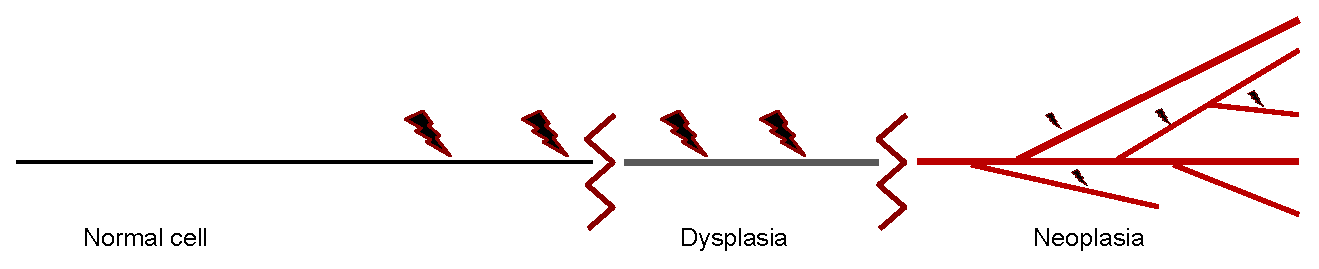
\includegraphics[width=0.95\linewidth,keepaspectratio]{images/intro/heterogeneity_diagram}
    \caption[Tumor heterogeneity arises from cancer mutation.]{Mutations can lead to cancer and intratumor heterogeneity. In a cancer case, the first neoplastic cell arises from mutations acquired in its genetic history. As cancer cells multiply, they have the capacity to diversify as different cancer cell subpopulations acquire different mutations. Lightning bolt symbols represent mutations.}
    \label{fig:intro:heterogeneity_diagram}
\end{figure}
An enormous variety of mutations can lead to cancer in any cell in the human body. Often, normal cells acquire multiple mutations (varying substantially among tumors) and pass through a pre-cancerous dysplastic stage on their way to neoplasia. However cancer cells do not stop mutating; rather each cancer cell is able to acquire mutations and found its own lineages of descendent cancer cells throughout the disease course, which leads to intertumor heterogeneity (Figure~\ref{fig:intro:heterogeneity_diagram}). Intertumor heterogeneity is believed to contribute to several aspects of cancer growth, progression, resistance to treatment, and metastasis \cite{mcgranahan2017}. Freed from the normal constraints on cell proliferation, cancer cells become subject to natural selection in the host organism. Cancer cells which acquire mutations permitting increased growth can grow to outcompete less aggressive cancer cell populations. Some mutations increase the capacity of a cancer cell to metastasize, for example via epithelial-mesenchymal transition \cite{zhang2018}. Metastatic cells encounter a different microenvironment than their tissue of origin, and this new evolutionary fitness landscape promotes microevolution for persistence and survival leading metastatic cancer cells to genetically diverge from the primary \cite{zeeshan2017}.

Tumors encounter opposition throughout their existence. This arises from natural causes, most notably the host immune system, as well as artificial causes \textit{i.e.}\ cancer treatment. To become established and grow, cancer cells must evade or suppress the immune system. However, mutations affecting coding regions of the genome run the risk of creating neoantigens, or immunogenic mutant protein regions which are selected against \cite{vitale2021}. Immune pressure also selects for immunosuppressive mechanisms such as PD-L1 upregulation \cite{kim2016}. Also substantially contributing to tumor heterogeneity are cancer treatments \cite{dagogojack2017}. Many cancer treatments are mutagenic (Section~\ref{ssec:intro:mutation}), producing additional mutations which provide additional chances for tumor microevolution and increased heterogeneity. Treatments also exert selective pressure on tumor cells, as mutations may confer differential sensitivity to treatment by a variety of mechanisms such as (but not limited to) tolerance of chemotherapy, resistance to targeted inhibitors, and escape from ligand dependence. This favors evolution of cells which can grow in spite of treatment, analogous to selection for drug-resistant bacteria with antibiotic therapy.

Single-cell experiments and computational modeling reveal that cancer cells on average acquire multiple mutations per cell division \cite{tsyvina2020,werner2020}. Given that a 1~cm\textsuperscript{3} tumor is estimated to comprise \textapprox{}10\textsuperscript{8} tumor cells \cite{monte2009}, this demonstrates the fantastic potential complexity of tumor heterogeneity. The concept of tumor \textbf{subclones}, first proposed by Dr.\ Peter Nowell in 1976 \cite{nowell1976}, has emerged as a useful paradigm for modeling tumor heterogeneity and evolution \cite{zhu2021}. A subclone represents a population of cancer cells genetically distinct from other subclones; although each cell in a subclone may have genetic differences, all cells in a subclone have genetic similarities characteristic of a common lineage.

\begin{figure}[tbh]
    \centering
    \begin{subfigure}{0.43\textwidth}
        \includegraphics[width=\linewidth,keepaspectratio]{images/intro/heterogeneity_example}
        \vspace{-0.5cm}
        \caption{}\label{fig:intro:heterogeneity_example}
    \end{subfigure}%
    \hspace{1cm}%
    \begin{subfigure}{0.31\textwidth}
        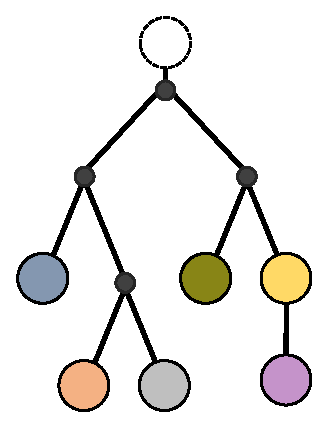
\includegraphics[width=\linewidth,keepaspectratio]{images/intro/tree_example}
        \vspace{-0.07cm}
        \caption{}\label{fig:intro:tree_example}
    \end{subfigure}
    \vspace{-0.3cm}
    \caption[Subclones can approximate intratumor heterogeneity.]{Subclones provide a useful model to approximate tumor heterogeneity. (\subref{fig:intro:heterogeneity_example}) Cancer cells within heterogeneous tumors are grouped into subpopulations termed subclones based on genetic similarity. Subclones are defined for an entire case of cancer, and each circled group of cells represents a separate tumor from a single patient, each comprised of different proportions of subclones. (\subref{fig:intro:tree_example}) Subclonal populations can be organized into a phylogenetic tree reflecting tumor microevolution and acquisition of mutations during the cancer's history. Figure in (\subref{fig:intro:heterogeneity_example}) is based on ``Cancerous cells'' by Les Laboratoires Servier, licensed under CC BY 3.0.}
    \label{fig:intro:subclones_example}
\end{figure}
Through the lens of subclones, intertumor heterogeneity can be approximated by relative proportions of subclonal populations in one or more tumor samples (Figure~\ref{fig:intro:heterogeneity_example}). Differences in subclone abundance among different sites of disease can implicate genes in these subclones as involved in metastasis and metastatic persistence, and shifts over time may reflect responses to treatment and outgrowth of resistant subclones. Furthermore, subclones provide a tractable model of tumor microevolution, as subclonal genotypes can be ordered into an estimated phylogeny (Figure~\ref{fig:intro:tree_example}). Such phylogenies approximate the evolutionary history of each subclone and infer ancestral subclones no longer extant in the available samples, permitting the researcher to estimate the relative timing of mutations during the disease course. Mutations can be divided into ``truncal'' or ``clonal'' mutations which are present in all subclones, and ``subclonal'' mutations found in only some subclones. Cancer treatments targeting truncal mutations may be more efficacious than those targeting subclonal mutations, as in theory all cancer cells would be sensitive (excepting resistance adaptations).

\subsection{Research methods}
\label{ssec:intro:heterogeneity_methods}
Intrapatient heterogeneity has been recognized since the beginnings of cancer treatment, with the observations that different cancers respond differently and possess different prognoses. Advances in cancer research and clinical practice have led to increasingly elaborate classifications of cancer. Currently the World Health Organization (WHO) system is used as a reference standard to classify cancers \cite{who_cancer_classification_1_5,who_cancer_classification_2_5,who_cancer_classification_3_5,who_cancer_classification_4_5}, a scheme which is increasingly incorporating genetic features \cite{carbone2020}. In addition, cancers are classified by stage, the size and extent of cancer in the body, and by grade, the extent of histological differences between tumor tissue and its original tissue type. The American Joint Committee on Cancer (AJCC) curates the TNM (tumor, lymph node, metastasis) system for most human cancer types \cite{amin2017}. However, even these complex classification strategies fail to fully reflect the genetic diversity present among cancers, and the precision medicine paradigm of genomics-guided care is becoming increasingly prevalent \cite{johnson2017}.

Intratumor heterogeneity was first recognized under the microscope, as cancer cells from the same tumor may have widely varying appearances. The genetic basis of intratumor heterogeneity was recognized as early as 1958 through observations of different quantities of genetic material in different cancer cells from the same tumor \cite{huxley1958,mcgranahan2017}. Advances in DNA sequencing and genomics (Section~\ref{sec:intro:genomics}) have provided tools for directly assessing heterogeneous cancer genetics.

The proliferation of NGS along with advancements in bioinformatics have led to the development of a multitude of algorithms to analyze mutation and/or CNV patterns to infer tumor subclones and estimate their evolutionary history \cite{tarabichi2021}. In the following chapters we make use of the software tools Canopy \cite{canopy} and SuperFreq \cite{flensburg2020} and introduce extensions to Canopy (Sections~\ref{ssec:240:subclonal_inference},~\ref{ssec:msiclones:subclonal_msi}). Subclonal inference remains a highly active area of research. In addition, subclonal analysis has yielded genomic findings such as identification of truncal mutations, however such analysis has yet to translate to substantive improvements in clinical practice.

Also key to studies of tumor heterogeneity is sample acquisition. Tumor samples are typically acquired through biopsies. Though clinically routine, biopsies have disadvantages as a research tool. They are invasive and carry clinical risks, such as infection and hemorrhage (often requiring anticoagulant medication to be held, in turn increasing risk of thromboembolism), and they cause inconvenience, discomfort and pain to the patient. A biopsy typically samples only a small portion of a single tumor, which may not be representative of the entire cancer. Such small quantities of tumor tissue also limit the analyses that can be performed. Surgical specimens (such as from resection and debulking surgeries) provide greater quantities of tumor tissue, but not all patients are surgical candidates and surgery may not remove all tumors from a patient.

\begin{figure}[tbhp]
    \centering
    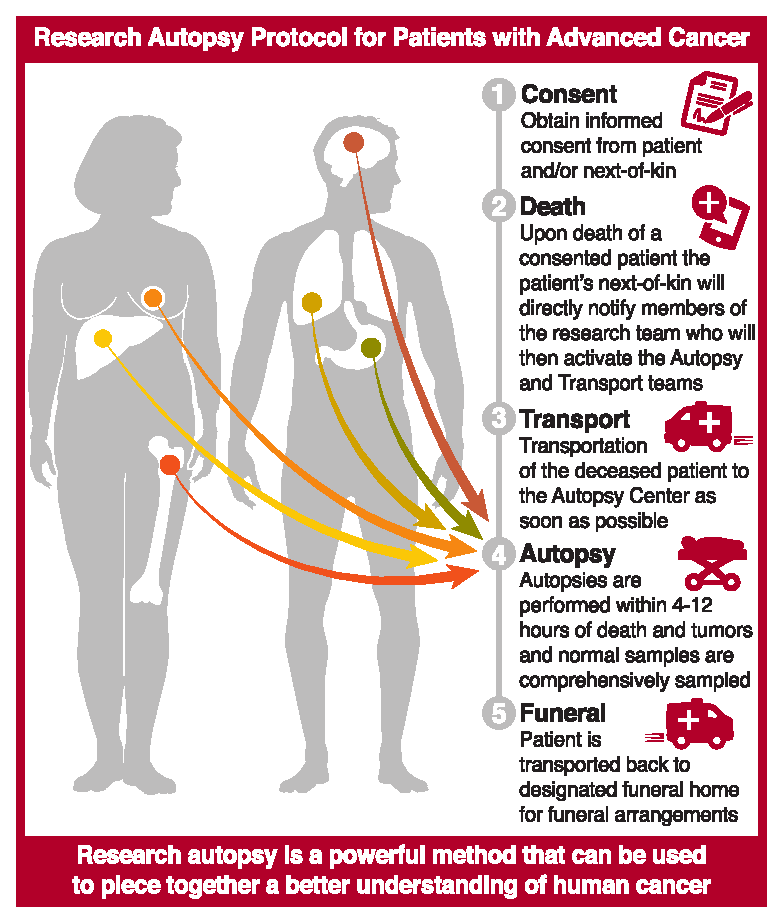
\includegraphics[width=0.7\textwidth,keepaspectratio]{images/intro/autopsy_puzzle_pieces}
    \vspace{-0.3cm}
    \caption[Research autopsy facilitates cancer research.]{Research autopsy facilitates cancer research by providing opportunities for comprehensive tumor sampling and analysis. This allows greater investigation into tumor heterogeneity and evolution, which provides insights into acquired resistance. When performed quickly enough, research autopsy can provide viable cells to create sustainable research resources such as cell lines.}
    \label{fig:intro:autopsy_puzzle_pieces}
\end{figure}
Because of these limitations, research into tumor heterogeneity is increasingly incorporating rapid research autopsy (also called warm autopsy) \cite{duregon2019}. Through collaboration between patients, clinicians, and researchers, patients with advanced cancers and terminal prognosis are provided the opportunity to consent to a rapid research autopsy study (Figure~\ref{fig:intro:autopsy_puzzle_pieces}) \cite{krook2019_review}. Upon notification of death, the decedent undergoes autopsy as soon as possible (ideally within 12 hours post-mortem) to best preserve nucleic acid integrity. A limited autopsy is performed by an on-call team consisting of pathologists and cancer researchers, with reference to previous imaging to extract tumor samples. Special attention is paid during the autopsy such that the patient and their family can receive an open-casket funeral if desired, and that the patient's funeral rites and customs are respected. The decedent is then transferred to the desired funeral home.

Though research autopsy permits comprehensive sampling of large tumor volumes throughout a patient, it can only acquire samples at one time point. Cancer mutates throughout the disease course, and the evolutionary history of tumors at autopsy can at best only be estimated through bioinformatics methods. Therefore, interest is growing in so-called ``liquid biopsies'' through circulating tumor DNA, or ctDNA \cite{merker2018}. Cancer cells release small amounts of their DNA into the bloodstream through a variety of processes, which can be isolated from a blood sample and sequenced \cite{gilson2020}. As blood draws are considerably cheaper, safer, and less invasive than tumor biopsies, ctDNA permits frequent sampling of DNA from tumors throughout the body. However ctDNA typically constitutes a low percent of the cell-free DNA (cfDNA) in the bloodstream and is typically found in very short fragments (even shorter than typically desired for NGS), which poses substantial technical challenges for sequencing and bioinformatics analysis. Additionally, ctDNA permits sampling from multiple tumors in theory, but much remains unknown regarding the relative contribution of different tumors in different locations to ctDNA, which is thought to consist of a complex interaction between genetics, cell turnover, tumor size, vascularity, and other factors \cite{haber2014}. A combination of research autopsy and ctDNA can provide greater insights than either method alone.

%patterns of heterogeneity (linear, branched, neutral, etc)?
%if section needs expanding, possibly subsections Concepts (above), Research Methods (biopsy, histology, autopsy, ctDNA), Current Findings (cite a few clonal papers, mention patterns of heterogeneity)
\section{Cancer as a dynamic process}
As we have seen, cancers acquire mutations throughout the disease course, with potential for substantial impacts on cancer behavior including progression, metastasis, and response to treatment. These in turn affect morbidity and mortality. Though a variety of CLIA (Clinical Laboratory Improvement Amendments)-certified genomics-based tests have been developed such as FoundationOne\textsuperscript\textregistered{} \cite{frampton2013}, Guardant360\textsuperscript\textregistered{} \cite{lanman2015} and OSU-SpARKFuse \cite{reeser2017}, it is impractical to test a patient on a sufficiently frequent basis to gain full awareness of the dynamic mutational landscape of his or her cancer. Even advancements in frequency and ease of testing are frustrated by tumor heterogeneity, which not only substantially increases the complexity of the mutational landscape but renders biopsies and other tumor samples inadequate to study an entire cancer in a patient. To overcome this will require an improved understanding of the temporal and spatial dynamics of cancer mutation, to facilitate empirical and quantitative models that would allow the researcher or clinician to predict and anticipate cancer mutations and their consequent effects on cancer biology. This will require extensive genomic studies, leveraging the power of `Big Data' to permit accurate development and validation of such complicated models.

In this work, we study microsatellite instability, introducing a new algorithm to quantify MSI in tumor samples and the prevalence of MSI across a wide cohort of cancers (Chapter~\ref{ch:msilandscape}). MSI is particularly well-suited to study from a temporal perspective, as MSI-related mutations typically arise at known locations in the genome (microsatellites) and their extent can be efficiently quantified through NGS\@. We provide multiple extensive studies of patients with advanced cancers through NGS and rapid research autopsy, in which we identify tumor subclones and relate these to cancer phenotypic features including treatment resistance (Chapters \ref{ch:240}, \ref{ch:303} and \ref{ch:sclc}). Finally, we develop a framework to quantify MSI within tumor subclones and apply this to a panel of cancers with MSI to quantify microsatellite mutation rates and dynamics in subclonal cancer populations (Chapter~\ref{ch:msiclones}). A fuller understanding of the dynamics of cancer genetics will require substantially greater research efforts, however we hope that the studies presented here will highlight the potential which studies of a cancer as a dynamic process may provide for improved understanding of cancer and clinical management.

\chapter[Microsatellite sequencing permits study of alterations in microsatellite unstable cancers]{Microsatellite sequencing permits study of alterations in microsatellite unstable cancers\footnote{This chapter previously published as: \begin{itemize} \item{Kautto E, Bonneville R, \textit{et al}. Performance evaluation for rapid detection of pan-cancer microsatellite instability with MANTIS\@. \textit{Oncotarget} 2016 [Epub 12 Dec 2016]} \item{Bonneville R\cofirst, Krook MA\cofirst, \textit{et al}. Landscape of microsatellite instability across 39 cancer types. \textit{JCO Precision Oncology} 2017 [Epub 3 Oct 2017]. Reprinted with permission. \textcopyright{} (2017) American Society of Clinical Oncology. All rights reserved.}\end{itemize}}}
\label{ch:msilandscape}

\section{Introduction}
Microsatellites are short (1--6 bp) repeating motifs, widely dispersed throughout the human genome \cite{kelkar2010}. Microsatellite instability (MSI) is a genetic phenomenon of somatic polymorphisms of microsatellite length, caused by uncorrected ``slippage'' of DNA fragments during DNA replication in cell division (Section \ref{ssec:intro:mutation}). MSI can arise from defects in the DNA mismatch repair (MMR) system \cite{shia2015}, which renders cells unable to regulate the lengths of their microsatellites during cell division. These defects may be inherited, as with Lynch syndrome/hereditary nonpolyposis colorectal cancer \cite{lynch1966,aaltonen1993}, or may be somatically acquired, most commonly due to promoter hypermethylation of the MMR gene \textit{MLH1} \cite{armaghany2012}. After multiple cycles of cell division, cells with an impaired MMR system will develop varying lengths in their microsatellite sequences.

Increasing evidence demonstrates that MSI is a recurrent somatic abnormality in several human cancers, previously described in 13\% of colorectal adenocarcinoma and 22-33\% of uterine/endometrial carcinoma \cite{dudley2016}. Reliable detection of MSI is clinically useful as patients with MSI-high (MSI–H) colorectal tumors have been shown to have improved prognosis over those with microsatellite stable (MSS) tumors \cite{buckowitz2005,benatti2005}. Furthermore, MSI-positive tumors appear more susceptible to immune-enhancing therapies, as observed in colorectal cancer for the PD-1 inhibitor pembrolizumab \cite{le2015}, recently approved for any MSI-H or MMR-deficient unresectable or metastatic solid tumor \cite{keytrudafda2017}. Thus far, MSI-H tumors have the highest response rates for any cancer types to PD-1 inhibitors, have durable responses, and a statistically significant improvement in overall survival.

The two currently accepted assays for the detection of MSI are MSI-PCR of five standardized microsatellite loci (Bethesda panel) \cite{boland1998}, and immunohistochemistry (IHC) of the MMR proteins MSH2, MSH6, MLH1 and PMS2. Traditionally, tumors can be classified with MSI-PCR as MSS (0/5 loci unstable), MSI-low (MSI-L, 1/5 loci unstable), or MSI-H ($\ge$2/5 loci unstable). However, both of these methods have inherent limitations. MSI-PCR relies on a small set of loci that were selected based on markers from a single disease type, potentially excluding loci that would be better predictors in other diseases and increasing the odds of incorrect classification \cite{boland1998}. Immunohistochemistry can be used to detect the expression of mismatch repair proteins, but does not directly look at the microsatellite loci. More recently, with the increasing prevalence of next-generation sequencing (NGS) in cancer biology, several computational methods have been developed using either colorectal or endometrial cancer NGS data to determine MSI status \cite{salipante2014,niu2013}.

The development, refinement, and validation of NGS-based computational MSI calling methods have several research and clinical applications. NGS allows for the practical assessment of far more microsatellite loci than MSI-PCR\@. Importantly, computational MSI analyses can be integrated into existing NGS pipelines for other mutation types such as single nucleotide variation or copy number variation, as well as applied to previously generated NGS data for retrospective analyses. As NGS increases in both cost-effectiveness and prevalence, NGS-based methods may permit identification of MSI status without requiring additional clinical testing or patient sample processing. Lastly, NGS data is becoming increasingly available in tumor types that are not routinely tested for MSI, with potential opportunities to identify microsatellite instability in previously uncharacterized cancers. Thus, there is a need to develop tools with high accuracy in multiple cancer types.

In this study, we introduce a new tool, MANTIS (Microsatellite Analysis for Normal Tumor InStability), for detecting MSI status from NGS data. We compare MANTIS with two currently available tools, mSINGS \cite{salipante2014} and MSISensor \cite{niu2013}, and test their performance across six different tumor types. We demonstrate that MANTIS achieves high sensitivity (97\%) and specificity (99\%) across six cancer types. We also determine that the number of loci assessed impacts the accuracy of MSI calling methods, and we find an optimal number of loci to analyze with each tool for best tool performance. As MANTIS performance is most stable with varying numbers of available loci, MANTIS is particularly well suited for application to a wider variety of cancer types.

Clinical MSI testing is routinely performed only on colorectal and endometrial tumors \cite{giardiello2014}, therefore the prevalence of MSI in many other cancer types has been much less well described. Additionally, evidence exists that MSI-PCR may be less accurate in other cancer types \cite{faulkner2004}. A recent study by Hause \textit{et al} \cite{hause2016} developed and applied the MSI detection tool MOSAIC to perform a detailed survey of MSI across 18 cancer types (n=5,930 cases). However, many other cancer types have yet to be analyzed for MSI\@. The ability to detect MSI in novel cancer types would permit investigation of immune-enhancing therapies in these cancers, with the potential to benefit previously unknown subsets of cancer patients with MSI\@.

To perform a more comprehensive assessment of MSI across many additional cancer types than analyzed by Hause \textit{et al}, we applied MANTIS to determine the prevalence of MSI in 39 distinct cancer types (n=11,139 tumors from 11,080 patients).

\section{Materials and Methods}

\subsection{MANTIS}
\label{ssec:msilandscape:mantis}
\begin{figure}[htp]
	\centering
	\includegraphics[width=\linewidth,keepaspectratio]{images/msilandscape/mantis_flowchart}
	\caption[Schematic of the MANTIS analysis for MSI detection.]{The schematic of the MANTIS analysis for MSI detection. Microsatellite loci are realigned against the reference genome to account for 0/1-based indexing differences. Per-locus microsatellite length distributions are determined from the normal and tumor BAM files by extracting locus-spanning reads; filtering out reads that fail to meet minimum length and average base quality requirements; determining the start position of the microsatellite motif within each read's sequence and the number of motif repeats; ensuring such reads meet minimum average locus quality and are not prematurely truncated in the middle of a motif repeat. The generated normal and tumor length distributions are evaluated at each locus, with outlying length values (by default, \textgreater{}~3~SD from mean) removed. Loci with substandard coverage are also removed. The support counts at each locus are then normalized separately for the normal and tumor sample and the stepwise difference between each distribution is calculated. Finally, the average of all difference scores is taken to generate the instability score for the normal-tumor sample pair.}
	\label{fig:msilandscape:mantis_flowchart}
\end{figure}
MANTIS is a tool for identifying microsatellite instability in paired tumor-normal patient samples (Figure~\ref{fig:msilandscape:mantis_flowchart}). It is written as a Python program, utilizing the NumPy (developed with version 1.6.2) \cite{2020NumPy-Array} and Pysam (developed with version 0.8.3) \cite{samtools} libraries. Additionally, it requires the reference genome in FASTA format to perform alignment of reads spanning the microsatellite loci. The matched normal and tumor inputs are required as indexed BAM files, aligned with any DNA sequence aligner. The targeted loci are required in a 6-column BED file, with the fourth column containing the motif of the microsatellite loci being targeted along with its repeat count in the reference genome, \textit{e.g.}\ \texttt{(AC)12}. MANTIS includes a bundled C\texttt{++} program, RepeatFinder, used to identify microsatellite loci within a reference genome, and create the appropriate BED file. This BED file can be further filtered with BEDTools \cite{quinlan2010} for regions of interest. Multi-threading is supported and encouraged for larger samples, but is not necessary. More information about the parameters supported by MANTIS is included in the manual available with the software.

Targeted loci are first read from the provided BED file and realigned against the provided reference genome to account for differences between 0- and 1-based indexing. One locus at a time, the tool extracts overlapping reads from the tumor and normal BAM files and performs an initial quality control step to ensure the reads are of sufficient sequence length, meet a minimum average base quality score, and cover the entire targeted locus. Reads passing the initial filtering step are inspected individually to determine the starting position of the microsatellite motif within the read's sequence and the total number of repeats is determined by pattern matching the continuous motif pattern from that starting point. Once the repeat count is determined, a secondary quality control step takes place, ensuring that the locus was not truncated before reaching the end of the read's sequence, and that the microsatellite locus region has a sufficiently high average base quality score. The supporting read count for each of the repeat lengths is determined separately for the tumor and normal files to generate per-locus motif repeat count values.

Once the repeat counts are generated for each locus, a per-locus quality control step takes place. The repeat lengths for both the normal and tumor file are evaluated separately, with values too far from the mean (by default, beyond 3 standard deviations) discarded as outliers. After outliers are removed, each locus is checked for a total number of supporting reads to ensure there is sufficient support to generate a statistically significant distribution for both the normal and tumor files. Loci with substandard coverage are discarded. 

The filtered locus repeat count data is then passed to the scoring algorithm that generates an instability score for the sample pair. First, each locus is evaluated separately, with the normal and tumor read distributions normalized to a fraction of each one's total reads, to account for any differences in sequencing depth and coverage. Then, absolute value of the stepwise difference between the tumor and normal distributions is determined:
\begin{equation}
	d=\sum_{r \in (R_T \cup R_N)} \left|T_r - N_r\right|
	\label{eqn:msilandscape:mantis_sum}
\end{equation}
where $d$ = distance score, $R_T$ = repeat counts present in tumor, $R_N$ = repeat counts present in normal, $T_r$ = normalized read count in tumor supporting repeat of length $r$, $N_r$ = normalized read count in normal supporting repeat of length $r$. Once the scores for each locus are assigned, the average of all the locus instability scores is calculated, to provide a single numerical value representing the average aggregate instability present in the sample. Scores reported range from 0.0 (entirely stable) to 2.0 (entirely unstable). The MANTIS software and manual are freely available for download at \url{https://github.com/OSU-SRLab/MANTIS}.

\subsection{Comparison of tools}
\begin{table}[H]
	\begin{center}
		\begin{tabular}{l|c|c|c}
			\textbf{Tool} & \textbf{Sample Comparison} & \textbf{Statistical Method} & \textbf{Scoring Approach} \\
			\hline
			\textbf{mSINGS} & Tumor vs.\ Baseline & Z-score & Per Locus \\
			\textbf{MSISensor} & Tumor vs.\ Normal & Chi-square & Per Locus \\
			\textbf{MANTIS} & Tumor vs.\ Normal & Average distance & Aggregate Instability
		\end{tabular}
	\end{center}
	\vspace{-0.3cm}
	\caption[Comparison of the MSI-calling tools mSINGS, MSISensor and MANTIS.]{Comparison of the MSI-calling tools mSINGS, MSISensor and MANTIS, and the algorithms used by each.}
	\label{table:msilandscape:tool_comparison}
\end{table}
In addition to MANTIS, we tested mSINGS (commit \verb|#2e00b6|) by Salipante \textit{et al} \cite{salipante2014} and MSISensor (version 0.2) by Niu \textit{et al} \cite{niu2013} (Table~\ref{table:msilandscape:tool_comparison}). mSINGS compares a tumor sample to a pooled normal baseline, generated from the distribution of unique alleles at each microsatellite locus in many normal samples. MSISensor, like MANTIS, compares a tumor sample with its matched normal sample. Both mSINGS and MSISensor determine the stability of each locus analyzed. mSINGS calls a locus unstable if the Z-score of the number of unique alleles at the locus relative to the baseline distribution exceeds a threshold (default: 2). MSISensor calls a locus unstable if a chi-square test of the repeat lengths in the tumor sample vs.\ the normal sample is statistically significant, after Benjamini correction for multiple hypotheses \cite{benjamini1995}. Both tools then call the sample MSI-H or MSS if the percentage of unstable loci exceeds a threshold.

\subsection{Tool parameters}
\label{ssec:msilandscape:tool_params}
mSINGS was run with Python 2.7.1, VarScan 2.3.6 \cite{varscan2} and SAMtools 0.1.18 \cite{samtools}. The wrapper script provided with mSINGS was modified to remove its dependency on SCons (\url{http://scons.org/}). We generated separate pooled normal baselines from all normal samples within a particular cancer type, according to the mSINGS documentation. The microsatellite loci-containing region BED and .intervals files packaged with mSINGS were used, which contained 2,539 loci, as they are appropriate for whole exome TCGA analyses according to the mSINGS documentation.

MSISensor was slightly modified to output sites that were not called with somatic microsatellite instability along with its other output files, and compiled from source. It was run over the test data with the following settings: single-threaded, minimal homopolymer size 1, and minimal microsatellite size 1. All other options were left at their defaults. The microsatellite loci-containing region BED file packaged with mSINGS was used for fairness of comparison, as well as to restrict MSISensor to exomic regions.

MANTIS was run over the test data with three threads. The recommended quality settings for whole exome data were used as described in the included MANTIS manual; min read quality 20, min locus quality 25, and min read length 35. The microsatellite BED file was derived from the one provided by mSINGS\@.

\subsection{Target loci selection}
\label{ssec:msilandscape:loci_selection}
\begin{table}[H]
	\begin{center}
		\begin{tabular}{l|r|r|r|r}
			\textbf{Type of} & \textbf{Number of} & \textbf{Min Repeats} & \textbf{Max Repeats} & \textbf{Mean Repeats} \\
			\textbf{Microsatellite} & \multicolumn{1}{l|}{\textbf{Loci}} & & & \\
			\hline
			Monomer & 2436 & 3 & 36 & 15.94 \\
			Dimer & 96 & 6 & 18 & 14.86 \\
			Trimer & 4 & 3 & 8 & 4.75 \\
			Tetramer & 2 & 7 & 8 & 7.5 \\
			Pentamer & 1 & 3 & 3 & 3
		\end{tabular}
	\end{center}
	\vspace{-0.3cm}
	\caption[Breakdown of target loci used for microsatellite status calling.]{Breakdown of target loci used for microsatellite status calling. The count and repeat range of each type is listed.}
	\label{table:msilandscape:target_loci}
\end{table}
The 2,539 target loci being analyzed were derived from the ones provided with mSINGS and captured in whole exome sequencing data sets, and used with all three tools. Most of the targeted loci (Table~\ref{table:msilandscape:target_loci}) were monomer homopolymers of adenine or thymine (95.08\%), with only 4.04\% of loci being repeats of dimers or longer polymers. This bias towards monomer repeats was expected since intronic mononucleotide repeats outnumber other repeat regions in the human genome \cite{toth2000}. 

\subsection{Testing data}
\label{ssec:msilandscape:testing_data}
To evaluate mSINGS, MSISensor, and MANTIS, we used data from six cancer types: 76 colon and rectal adenocarcinomas (COAD/READ) \cite{tcgacoadread}, 99 uterine corpus endometrial carcinomas (UCEC) \cite{tcgaucec}, 100 gastric adenocarcinomas (STAD) \cite{tcgastad}, 71 esophageal carcinomas (ESCA), 53 uterine carcinosarcomas (UCS) \cite{tcgageneric}, and 59 prostate adenocarcinomas (PRAD) \cite{robinson2015}. Cancer type abbreviations are listed in Appendix~\ref{app.cancerabbrev}. We define a ``sample'' as a single BAM and its accompanying BAI index file, for a tumor or a normal. We define a ``pair'' as two samples; a tumor and its matched normal, and define a ``cohort'' as all samples within a cancer type, for a total of 6 cohorts (Table~\ref{table:msilandscape:test_samples_count}).

Data for all cohorts except PRAD were downloaded from the Cancer Genomics Hub (CGHub), using the CGHub-provided client GeneTorrent \cite{wilks2014}. All samples were downloaded in the BAM format, pre-aligned to GRCh37/hg19 \cite{lander2001}. 76 COAD/READ pairs were downloaded, comprised of 38 MSI-H and 38 MSS\@. COAD/READ data was sequenced at the Baylor College of Medicine (BCM) and the Washington University Genome Sequencing Center (WUGSC) (Table~\ref{table:msilandscape:test_samples_bycenter}). 99 UCEC pairs were downloaded, comprised of 49 MSI-H and 50 MSS\@. All UCEC pairs were sequenced at WUGSC\@. Next, 100 STAD pairs were downloaded; 50 MSI-H and MSS\@. All STAD pairs were sequenced at the Broad Institute of MIT and Harvard (BI)\@. The primary authors were blinded to the MSI status of these samples until after initial analysis with mSINGS, MSISensor and MANTIS was completed. Finally, 71 ESCA pairs were downloaded from TCGA; 2 MSI-H and 69 MSS, and 53 UCS pairs were downloaded; 2 MSI-H and 51 MSS\@. All ESCA and UCS pairs were sequenced at BI\@. PRAD data was downloaded from the Database of Genotypes and Phenotypes (dbGaP) (accession phs000915.v1.p1) \cite{mailman2007} as FASTQ files, using the SRA toolkit \cite{leinonen2010sra}. All 59 available PRAD pairs were downloaded; 1 MSI positive and 58 MSI negative (according to the original study for which these samples were sequenced, which only differentiated between MSI positive and MSI negative). PRAD data was sequenced at BI and the University of Michigan (UM) (Table~\ref{table:msilandscape:test_samples_bycenter}). Alignment to hg19 was performed with with Burrows-Wheeler Aligner (BWA) 0.6.2 \cite{bwa}.

Each of the 916 BAM files (from the 458 tumor-normal pairs in all six cancer types) were sorted and indexed with SAMtools 0.1.18. Deduplication was performed with Picard Tools 1.84 \cite{Picard2019toolkit}, and facilitated with GNU Parallel \cite{tange2011}. The deduplicated BAM files were used for all downstream analyses. Samples used in these analyses are summarized in Supplemental File~S\thechapter{}.1.

\subsection{Tool performance evaluation}
mSINGS, MSISensor and MANTIS were first run on all 175 tumor-normal pairs from COAD/READ and UCEC (Supplemental File~S\thechapter{}.2). A threshold was used for each tool, above which a tumor-normal pair is called MSI positive. For mSINGS, 0.2 (20\% of loci called unstable) was used as the threshold for differentiation of MSI positive from MSS predictions, as this is consistent with both MSI-PCR scoring and the threshold used by Salipante \textit{et al}. A threshold of 3.5\% (of loci called unstable) was used for MSISensor, as recommended by Niu \textit{et al}. For MANTIS, a threshold of 0.4 (average of loci difference scores \textgreater{}~0.4) performed best in testing (Section~\ref{ssec:msilandscape:tool_accuracy}), and was used for other analyses. For each tool, the number of true positives, false positives, true negatives, and false negatives was calculated with respect to MSI-PCR status as a gold standard, and this was used to calculate the sensitivity, specificity, error rate, and accuracy of each tool both overall and within each cancer type. Error rate was calculated as $\text{incorrect calls} / \text{total calls}$, and accuracy as $1-\text{error rate}=\text{correct calls} / \text{total calls}$. Note that error rate and accuracy depend on the samples being tested, and cannot be generalized to other data sets, as can sensitivity and specificity. 95\% confidence intervals for sensitivity and specificity were calculated using the Wilson score interval with continuity correction \cite{newcombe1998}. In addition, ranges of thresholds were tested for all three tools in order to determine which thresholds provided optimal performance with the COAD/READ and UCEC test data, allowing comparison of best-case performance. 300 thresholds ranging from 0.001 to 0.3 were tested for mSINGS, 400 thresholds ranging from 0.1\% to 40\% were tested for MSISensor, and 600 thresholds ranging from 0.001 to 0.6 were tested for MANTIS\@. After a threshold of 0.4 was chosen for MANTIS, we ran mSINGS, MSISensor and MANTIS over the 100 STAD, 71 ESCA, 53 UCS and 59 PRAD tumor-normal pairs. Tool parameters were selected and performance analyses were performed as described earlier.

For each tool, we measured potential bias arising from differences in sequencing and alignment protocols at different sequencing centers. In addition to the sample data used for tool performance comparison, TCGA data from 4 tumor-normal COAD/READ MSI-H pairs sequenced at both BI and BCM, as well as from 20 tumor-normal UCEC MSI-H pairs sequenced at both BI and WUGSC, was downloaded and preprocessed as earlier (Section~\ref{ssec:msilandscape:testing_data}) (Supplemental File~S\thechapter{}.3). After deduplication, these pairs were analyzed with mSINGS, MSISensor and MANTIS\@. MSISensor and MANTIS were run with the parameters described earlier (Section~\ref{ssec:msilandscape:tool_params}). For mSINGS, the normal BAM files were used to generate separate baselines for each cancer type and sequencing center.

In addition to evaluating the statistical performance of each tool, we also evaluated their computational performance. All three tools were profiled with the runtime and memory usage metrics supplied by the PBS (Portable Batch System) cluster queueing system. MSISensor and MANTIS were tested with one and three threads to evaluate changes in performance (mSINGS does not support multithreading).

\subsection{Loci number comparison}
\label{ssec:msilandscape:loci_number_comparison}
For each of the three tools tested, the top-performing 10, 20, 30, 40, 50, 100, 250, 500 and 1000 microsatellite loci within the COAD/READ, UCEC and STAD samples were determined, individually within each cancer type and across all three cohorts. ESCA, UCS and PRAD were not included in this as only five MSI-H cases were available from these cancer types. To determine the top $n$ loci for mSINGS and MSISensor, the accuracy of each locus was calculated as if only that locus were to be used to call the MSI status of each tumor sample. For MANTIS, since it calculates instability scores instead of assigning per-locus stability statuses, a difference of averages was calculated for each locus, defined as:
\begin{equation}
	a = \frac{\sum_{i \in H} d_i}{\left|H\right|} - \frac{\sum_{i \in S} d_i}{\left|S\right|}
\end{equation}
where $a$ = difference of averages, $H$ = set of MSI-H samples that cover the locus, $S$ = set of MSS samples that cover the locus, and $d_i$ = distance score of the locus in sample $i$. To compensate for varying locus coverage across samples, this score (accuracy or difference of averages) was then multiplied by the square of the proportion of pairs that had sufficient read coverage at that locus to consider it, as follows:
\begin{equation}
	l = ac^2
\end{equation}
where $l$ = locus score, $a$ = accuracy or difference of averages, and $c$ = proportion of samples that cover the locus. This yielded a performance score for each locus, which allowed all 2,539 loci to be ranked. The sensitivity, specificity, error rate, and accuracy of each tool with each loci list was then calculated, both for all three of these cancer types and overall (Supplemental File~S\thechapter{}.4).

\subsection{Landscape data preprocessing}
\subsubsection{L-MAP: Landscape Microsatellite Analysis Pathway}
\begin{figure}[htp]
	\centering
	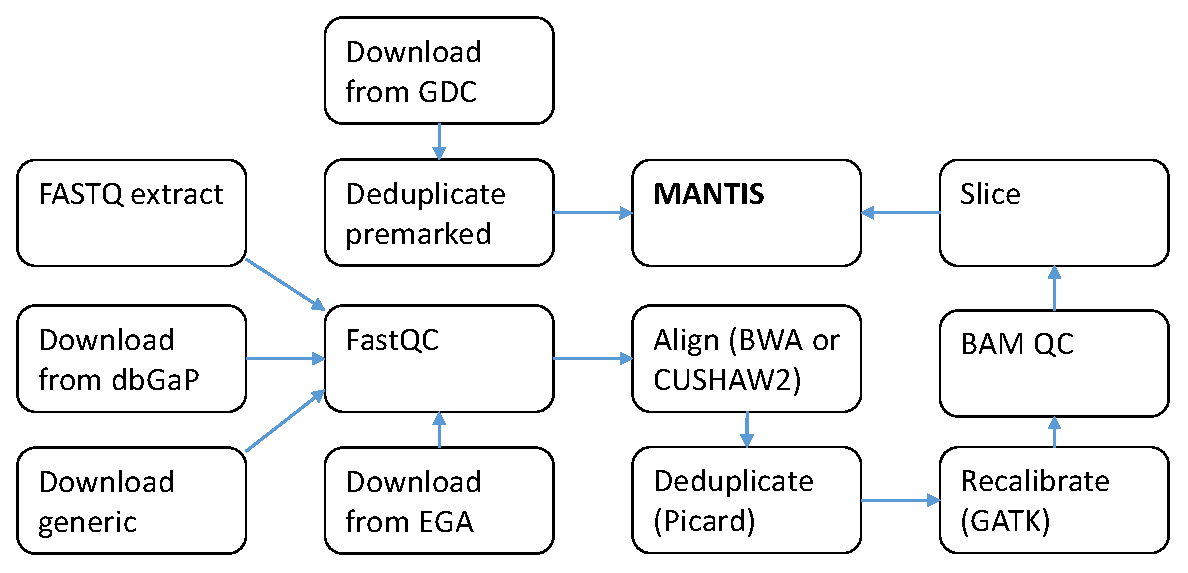
\includegraphics[width=0.8\linewidth,keepaspectratio]{images/msilandscape/lmap_flowchart}
	\caption[Schematic of L-MAP for bulk MSI analysis.]{Schematic of L-MAP (Landscape Microsatellite Analysis Pathway), an automated pipeline developed for bulk calling of microsatellite instability within large genomc data sets.}
	\label{fig:msilandscape:lmap_flowchart}
\end{figure}
To facilitate bulk processing and analysis of microsatellite instability, we developed an in-house automated pipeline, L-MAP (Figure~\ref{fig:msilandscape:lmap_flowchart}). L-MAP is implemented in Python and MySQL\@. L-MAP periodically polls a MySQL database for pending tasks in a pre-specified pipeline, and submits jobs to the PBS scheduler while respecting defined resource limits (concurrent batch jobs, cumulative storage utilization). Task types are specified in a MySQL table, with primary:foreign key pairs used to specify job dependencies. L-MAP supports input from available FASTQ files, along with automated downloads from generic URLs, dbGaP, the Genomic Data Commons (GDC) \cite{grossman2016}, and the European Genome-Phenome Archive (EGA) \cite{lappalainen2015}. QC metrics are computed for acquired FASTQs using FastQC \cite{fastqc}. Alignment is supported using BWA \cite{bwa} for Illumina reads and CUSHAW2 \cite{liu2012} for ABI SOLiD color-space reads (not used in this study). Reads are deduplicated with Picard MarkDuplicates \cite{Picard2019toolkit}, or pre-marked duplicates removed with SAMtools. Quality score recalibration and local realignment of reads around indels are performed with Genome Analysis Toolkit (GATK) \cite{mckenna10}. Additional basic QC measures (such as alignment percentage) are computed, and BAM files are sliced using SAMtools to retain only reads covering microsatellite regions to conserve storage space. Finally, MSI status is computed for tumor-normal sequencing pairs with MANTIS and MSISensor.

\subsubsection{TCGA and TARGET}
10,701 cases of paired tumor-normal whole exome sequencing data were obtained from The Cancer Genome Atlas (TCGA) \cite{tcgacoadread,tcgaucec,tcgastad,tcgaov,tcgabrca,tcgalaml,tcgakirc,tcgagbm,tcgablca,tcgaluad,tcgalusc,hoadley2014,tcgakich,tcgathca,tcgahnsc,tcgalgg,tcgaskcm,ciriello2015,tcgakirp,tcgaprad,tcgaacc,tcgaesca,tcgacesc,tcgapcpg} and Therapeutically Applicable Research to Generate Effective Treatments (TARGET) \cite{target,targetnbl} projects. Data from all of these cases except diffuse large B-cell lymphoma (DLBC) were processed through L-MAP\@. First, the metadata for all DNA whole exome BAM files was downloaded from GDC, and was converted to SQL database entries. Aligned BAM files (to hg38 \cite{lander2001}) were queried from GDC by L-MAP using the slicing endpoint provided by the GDC REST API\@. Reads covering any base within 50 base pairs (bp) of a desired microsatellite locus were downloaded. As GDC data harmonization includes duplicate marking, premarked duplicate reads were removed using SAMtools (version 1.3.1).

Due to a GDC sample contamination issue, all 48 DLBC paired tumor-normal cases were downloaded from the GDC Legacy Archive as whole exome BAM files aligned to hg19, using the GDC Data Transfer Tool, and separately analyzed. Premarked duplicate reads were removed as above.

\subsubsection{Other sources}
430 cases of paired tumor-normal whole exome sequencing data were obtained from the Sequence Read Archive \cite{leinonen2010sra}: 338 chronic lymphocytic leukemia (CLL) cases from 279 patients from Landau \textit{et al} \cite{landau2015}, 32 cutaneous T-cell lymphoma (CTCL) cases from Choi \textit{et al} \cite{choi2015}, 51 nasopharyngeal carcinoma (NPC) cases from Zheng H \textit{et al} \cite{zheng2016}, and 8 cholangiocarcinoma (CHOL) cases from Ong \textit{et al} \cite{ong2012}. 15 additional CHOL cases were obtained from the European Nucleotide Archive \cite{leinonen2010ena}, from Chan-on \textit{et al} \cite{chanon2013}. All sample identifiers used are available in Supplemental File~S\thechapter{}.5. These cases were processed through L-MAP\@. Tumor and normal samples were downloaded in the FASTQ format using fastq-dump \cite{leinonen2010sra}. Alignment to hg38 was performed using BWA (version 0.7.12) \cite{bwa} with the mem algorithm. Duplicate reads were marked and removed using Picard MarkDuplicates. Base quality score recalibration and indel realignment were performed using GATK, and the resulting BAM files were sliced (as above) using SAMtools.

\subsection{MSI calling --- landscape}
MSI analysis with MANTIS (version 1.0.3, commit \#942061f) was performed for all cases, using an average distance threshold of 0.4 to differentiate MSI-H from MSS tumors. The set of 2,539 coordinates within or near the exome used for MANTIS validation (Section~\ref{ssec:msilandscape:loci_selection}) were converted from hg19 to hg38 using UCSC LiftOver \cite{hinrichs2006}. Nine unlifted loci were discarded, leaving 2,530 regions that were used for analysis with MANTIS in all cohorts except DLBC (Supplemental File~S\thechapter{}.6). As the DLBC data was aligned to hg19, the original 2,539 loci were used instead. MANTIS was run with author-recommended settings for whole exome data (Section~\ref{ssec:msilandscape:tool_params}), with all other settings left at defaults. Eight samples were found to have fewer than 10 loci sufficiently covered, and were dropped from further analysis. After MSI calling, microsatellite locus performance was assessed in each cancer type as described above (Section~\ref{ssec:msilandscape:loci_number_comparison}). Kernel density estimation functions were computed using R (version 3.3.2), using the \texttt{density()} function with default settings.

\subsection{Whole exome analysis}
For all tumor-normal pairs tested by MANTIS in ACC (n = 92), CESC (n = 305), and MESO (n = 83), we downloaded aligned reads from whole exome sequencing. Reads were downloaded in BAM format from GDC, using the GDC Data Transfer Tool. Premarked duplicate reads were removed using SAMtools, variant calling was performed using MuTect \cite{cibulskis2013}, and annotation was performed using ANNOVAR \cite{annovar} (version 2016-02-01) and GNU Parallel.

\subsection{Variant calling}
\label{ssec:msilandscape:variant_calling}
All variant calling was performed using MuTect version 1.1.7. The target region was derived from RefSeq \cite{oleary2015} release 80. Exon data from the refGene table of the RefSeq Genes track was downloaded in BED format on February 28, 2017, using the UCSC Table Browser \cite{karolchik2004} and 100 bp padding. Unknown contigs were excluded, and overlapping regions were merged with BEDTools. VCF output was specified for MuTect, and all other options were left at their defaults. MuTect VCF output was then filtered for variants marked PASS\@. Variant annotation was performed using ANNOVAR and GNU Parallel. Somatic mutations in the DNA repair genes \textit{MSH2}, \textit{MSH6}, \textit{MLH1}, \textit{PMS2}, \textit{EXO1}, \textit{POLD1}, and \textit{POLE} were determined by filtering variants with a DANN \cite{quang2015} pathogenicity score above 0.96 (included in ANNOVAR)\@. This threshold for DANN was chosen as it was previously shown to provide optimal sensitivity and specificity \cite{jensen2015}.

Mutational signature calling was performed using the tool deconstructSigs \cite{rosenthal16}, with the Nature 2013 signatures set (containing 27 signatures) \cite{alexandrov2013} and ``exome2genome'' normalization method. A mutational signature is a probability vector of length 96, with each element representing a single base change, along with the bases immediately flanking it. In this analysis, non-negative linear regression is used to determine the relative contribution of each signature to the observed pattern of mutations. deconstructSigs was run over every ACC, CESC, and MESO sample, using all passing variants called with MuTect.

\subsection{Computing resources}
Alignment, deduplication, MSI calling with all three tools, tool performance calculations, and all landscape analyses (including L-MAP) were performed on the Oakley supercomputer at the Ohio Supercomputer Center \cite{Oakley2012}. Figures were generated using GraphPad Prism\textsuperscript\textregistered{} and Microsoft\textsuperscript\textregistered{} Excel\textsuperscript\texttrademark{} 2010. All other calculations were performed with custom Perl and Python scripts, R, and Excel\textsuperscript\texttrademark{}.

\section{Results}
\subsection{Evaluation of tool accuracy for detecting MSI status}
\label{ssec:msilandscape:tool_accuracy}
\begin{figure}[htp]
	\centering
	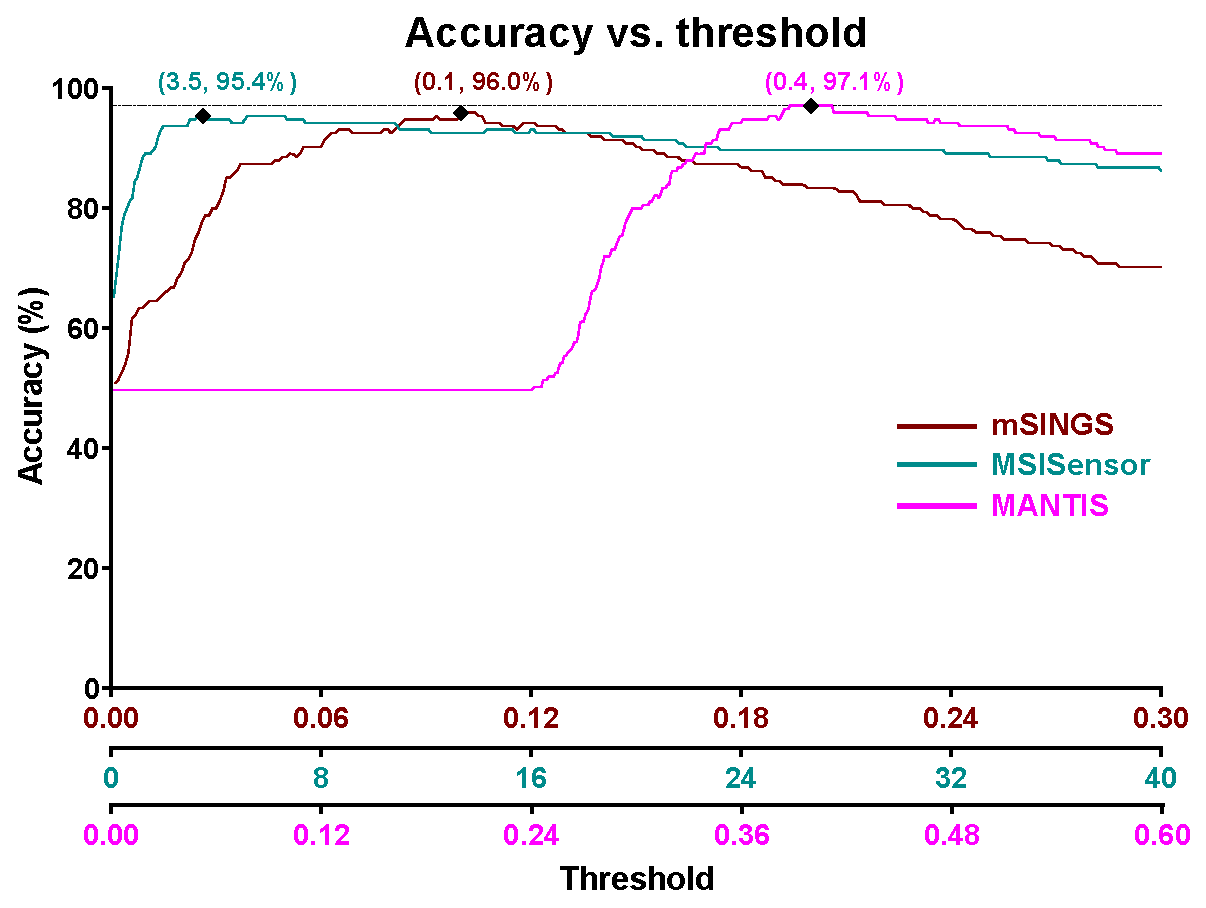
\includegraphics[width=\linewidth,keepaspectratio]{images/msilandscape/tool_thresholding}
	\caption[Accuracy of mSINGS, MSISensor and MANTIS at a range of thresholds.]{Accuracy of mSINGS, MSISensor and MANTIS at a range of thresholds, when tested with the 76 COAD/READ tumor-normal pairs and 99 UCEC tumor-normal pairs. The thresholds for each tool yielding the highest accuracy for the test data are highlighted. For mSINGS, thresholds from 0.001 to 0.3 were evaluated, in increments of 0.001. For MSISensor, thresholds from 0.1 to 40.0 were evaluated, in increments of 0.1. For MANTIS, thresholds from 0.001 to 0.6 were evaluated, in increments of 0.001.}
	\label{fig:msilandscape:tool_thresholding}
\end{figure}
Since mSINGS and MSISensor were each developed on data from single disease cohorts (COAD/READ for mSINGS, UCEC for MSISensor), the two cohorts were used for tool performance comparisons. To account for the possibility of suboptimal recommended cutoff thresholds for each of the three tools, we tested a range of thresholds for each tool across a test cohort consisting of both the COAD/READ and UCEC sample pairs (Figure~\ref{fig:msilandscape:tool_thresholding}). The peak performances of each tool were determined, with MANTIS having 97.1\% accuracy with the default threshold of 0.4, mSINGS reaching 96\% accuracy with a threshold of 0.1, and MSISensor peaking at 95.4\% accuracy with the threshold of 3.5\%. The results indicate that MANTIS demonstrated superior performance over the other tools, even after accounting for the best-case thresholds of the tools.

\begin{figure}[htp]
	\centering
	\includegraphics[width=0.5\linewidth,keepaspectratio]{images/msilandscape/mantis_coad_read_ucec}
	\caption[Distribution of MANTIS scores for COAD/READ and UCEC combined tumor-normal pairs.]{The distribution of MSI scores reported by MANTIS for the combined cohorts of 76 COAD/READ tumor-normal pairs and 99 UCEC tumor-normal pairs. The dotted line is at the threshold (0.4) to call a tumor MSI positive.}
	\label{fig:msilandscape:mantis_coad_read_ucec}
\end{figure}
Having evaluated the tools with the best-case thresholds, their performances were evaluated with the tool's recommended default cutoff thresholds (MANTIS 0.4, mSINGS 0.2, and MSISensor 3.5\%) (Figure~\ref{fig:msilandscape:mantis_coad_read_ucec}). MANTIS demonstrated the highest classification accuracy (97.1\%), followed by MSISensor (95.4\%), and mSINGS (83.4\%). MANTIS and MSISensor both exhibited equally high sensitivity (95.4\%). In contrast, although mSINGS was the most specific (100\%), it demonstrated poor sensitivity (66.7\%), largely due to poor performance over the UCEC cohort (53.1\% sensitivity). MANTIS also exhibited high specificity (98.9\%), performing better than MSISensor (95.5\%).

\begin{figure}[htp]
    \centering
    \begin{subfigure}{0.8\textwidth}
        \includegraphics[width=\textwidth,keepaspectratio]{images/msilandscape/perf_coadread_ucec_msings}
        \caption{}\label{fig:msilandscape:perf_coadread_ucec_msings}
    \end{subfigure}\par
    \begin{subfigure}{0.8\textwidth}
        \includegraphics[width=\textwidth,keepaspectratio]{images/msilandscape/perf_coadread_ucec_msisensor}
        \caption{}\label{fig:msilandscape:perf_coadread_ucec_msisensor}
    \end{subfigure}\par
    \begin{subfigure}{0.8\textwidth}
        \includegraphics[width=\textwidth,keepaspectratio]{images/msilandscape/perf_coadread_ucec_mantis}
        \caption{}\label{fig:msilandscape:perf_coadread_ucec_mantis}
    \end{subfigure}
    \caption[Distribution of MSI scores from all three tools in COAD/READ and UCEC.]{The cumulative distribution of MSI scores reported by mSINGS (\subref{fig:msilandscape:perf_coadread_ucec_msings}), MSISensor (\subref{fig:msilandscape:perf_coadread_ucec_msisensor}), and MANTIS (\subref{fig:msilandscape:perf_coadread_ucec_mantis}) for the 76 COAD/READ tumor-normal pairs and 99 UCEC tumor-normal pairs. The dotted lines are at the tools' respective thresholds to call a tumor MSI positive.}
    \label{fig:msilandscape:perf_coadread_ucec}
\end{figure}
To analyze disease-specific differences, results were compared between the COAD/READ and UCEC cohorts (Table~\ref{table:msilandscape:tool_accuracy}, Figure~\ref{fig:msilandscape:perf_coadread_ucec}). MANTIS produced more accurate results (98.7\%) than mSINGS (92.1\%) and MSISensor (92.1\%) in COAD/READ, whereas MSISensor was slightly more accurate (98.0\%) than MANTIS (96.0\%) in UCEC\@. While all three tools performed well with the COAD/READ data, mSINGS performed poorly with the UCEC data (accuracy 76.8\%, sensitivity 53.1\%). The tests showed that MANTIS had the most consistently accurate performance among the test cohort, exhibiting high sensitivity (95.4\%) and specificity (98.9\%) among the tested samples.

\subsection{Consideration of data overfitting and bias}
\begin{table}[H]
	\begin{center}
		\begin{tabular}{l|l|l|l|l}
			\multicolumn{5}{c}{\textbf{mSINGS}} \\
			\hline
			\textbf{Metric} & \textbf{COAD/READ} & \textbf{UCEC} & \textbf{COAD/READ} & \textbf{STAD} \\
			& & & \textbf{\& UCEC} & \\
			\textbf{Sensitivity} & 84.2\% & 53.1\% & 66.7\% & 92.0\% \\
			\textbf{Specificity} & 100.0\% & 100.0\% & 100.0\% & 100.0\% \\
			\textbf{Accuracy} & 92.1\% & 76.8\% & 83.4\% & 96.0\% \\
			\hline\hline
			\multicolumn{5}{c}{\textbf{MSISensor}} \\
			\hline
			\textbf{Metric} & \textbf{COAD/READ} & \textbf{UCEC} & \textbf{COAD/READ} & \textbf{STAD} \\
			& & & \textbf{\& UCEC} & \\
			\textbf{Sensitivity} & 92.1\% & 98.0\% & 95.4\% & 98.0\% \\
			\textbf{Specificity} & 92.1\% & 98.0\% & 95.5\% & 100.0\% \\
			\textbf{Accuracy} & 92.1\% & 98.0\% & 95.4\% & 99.0\% \\
			\hline\hline
			\multicolumn{5}{c}{\textbf{MANTIS}} \\
			\hline
			\textbf{Metric} & \textbf{COAD/READ} & \textbf{UCEC} & \textbf{COAD/READ} & \textbf{STAD} \\
			& & & \textbf{\& UCEC} & \\
			\textbf{Sensitivity} & 100.0\% & 91.8\% & 95.4\% & 100.0\% \\
			\textbf{Specificity} & 97.4\% & 100.0\% & 98.9\% & 100.0\% \\
			\textbf{Accuracy} & 98.7\% & 96.0\% & 97.1\% & 100.0\% \\
			\hline\hline
		\end{tabular}
	\end{center}
	\vspace{-0.3cm}
	\caption[Comparison of tool accuracy for MSI-H detection.]{Comparison of tool accuracy for MSI-H detection. The performance of mSINGS, MSISensor, and MANTIS over 275 COAD/READ, UCEC, and STAD sample pairs.}
	\label{table:msilandscape:tool_accuracy}
\end{table}

\begin{figure}[htp]
	\centering
	\includegraphics[width=0.95\linewidth,keepaspectratio]{images/msilandscape/scores_dist_entire_cohort}
	\caption[Distribution of MSI scores reported by mSINGS, MSISensor, and MANTIS.]{The cumulative distribution of MSI scores reported by mSINGS, MSISensor, and MANTIS for 275 COAD/READ, UCEC and STAD tumor-normal data pairs. The dotted lines are the tools' respective thresholds to call a tumor MSI positive.}
	\label{fig:msilandscape:scores_dist_entire_cohort}
\end{figure}
To further evaluate tool performance and to ensure MANTIS was not overfit to the COAD/READ and UCEC cohorts, tool performance was evaluated using stomach adenocarcinoma (STAD) sample pairs as a blinded test cohort (Figure~\ref{fig:msilandscape:scores_dist_entire_cohort}). All three tools performed well with the STAD data, with MANTIS performing the best with 100\% accuracy, followed by MSISensor with 99\% accuracy and mSINGS with 96\% accuracy (Table~\ref{table:msilandscape:tool_accuracy}).

To evaluate the extent that tool performance was affected by differences in sequencing, samples that had been sequenced at different sequencing centers with potentially different protocols and practices, were compared. For the comparison, we evaluated tool performance on a selection of MSI-H sample pairs that were each sequenced at two different centers (Table~\ref{table:msilandscape:test_results_by_site}). All three tools showed high concordance ($r^2 > 0.99$ in all cases) for the 20 UCEC tumor-normal pairs used in these comparisons. For the 4 COAD/READ pairs, MSISensor and MANTIS showed high concordance ($r^2 > 0.99$), however no concordance was observed with mSINGS ($r^2 = 5.52 \times 10^{-7}$). This indicated that while MANTIS and MSISensor are less affected due to their paired normal-tumor comparison model, mSINGS requires a statistically large enough population to generate a baseline from.

Finally, to assess the potential utility of MANTIS as well as other tools for pan-cancer MSI analysis, we tested MANTIS, mSINGS, and MSISensor with three additional cohorts of cancer: esophageal carcinoma (ESCA), uterine carcinosarcoma (UCS), and prostate adenocarcinoma (PRAD) (Table~\ref{table:msilandscape:detailed_perf}). All three tools reached 100\% accuracy with ESCA, and MSISensor and MANTIS were 100\% accurate with UCS and PRAD\@. However, mSINGS only reached 50\% sensitivity (and 98.1\% accuracy) with UCS data, and had one false positive in PRAD (98.3\% specificity and 98.3\% accuracy). Testing with these four additional disease cohorts further confirmed the accuracy of MANTIS, showing it may have superior pan-cancer applicability over the other two tools being compared.

\subsection{Computational performance}
\begin{table}[H]
    \footnotesize
	\begin{center}
		\begin{subtable}{0.93\textwidth}
			\begin{tabular}{l:rr}
				\textbf{File} & \textbf{File size (bytes)} & \textbf{Total reads} \\
				\hline
				TCGA-V5-A7RE-11A-11D-A351-09.rmdup.bam (normal) & 11554546055 & 82966335 \\
				TCGA-V5-A7RE-01A-11D-A351-09.rmdup.bam (tumor) & 10689033275 & 76367232
			\end{tabular}
			\caption{}\label{table:msilandscape:comp_performance_samples}
		\end{subtable}
		
		\begin{subtable}{0.93\textwidth}
			\begin{tabular}{l:lllll}
				& \textbf{mSINGS} & \textbf{MSISensor} & \textbf{MSISensor} & \textbf{MANTIS} & \textbf{MANTIS} \\
				& & \textbf{1 thread} & \textbf{3 threads} & \textbf{1 thread} & \textbf{3 threads} \\
				\hline
				\textbf{Runtime} & 26:44 & 4:10 & 4:42 & 2:56 & 2:20 \\
				\textbf{Maximum memory} & 1.48 GB & 38 MB & 30 MB & 89 MB & 108 MB \\
				\textbf{usage} & & & & & \\
				\textbf{Disk space} & 32 GB & 2.3 MB & 2.3 MB & 896 KB & 896 KB \\
				\textbf{(intermediate files} & & & & & \\
				\textbf{and results)} & & & & &
			\end{tabular}
			\caption{}\label{table:msilandscape:comp_performance_resources}
		\end{subtable}
	\end{center}
	\vspace{-0.3cm}
	\caption[Performance profiling of mSINGS, MSISensor and MANTIS.]{Performance profiling of mSINGS, MSISensor and MANTIS over a representative tumor-normal pair (TCGA-V5-A7RE)\@. In (\subref{table:msilandscape:comp_performance_samples}), the file size of each BAM and total number of reads after deduplication is listed. In (\subref{table:msilandscape:comp_performance_resources}), runtime, memory usage, and total disk space used by each tool is listed. Runtime is listed as minutes:seconds. mSINGS runtime does not include baseline generation. As MSISensor and MANTIS support multithreading, one thread and three threads were tested for each.}
	\label{table:msilandscape:comp_performance}
\end{table}
Since resource limitations can affect the rate at which computational analysis of samples can be performed, we used the tumor and normal samples of TCGA-V5-A7RE (a known ESCA MSS case) for evaluating the computational performance of the three tools, as both deduplicated BAM files were close to 10~GB in size. We found that mSINGS performs considerably slower than MSISensor and MANTIS, with runtime at least five-fold longer (Table~\ref{table:msilandscape:comp_performance}). mSINGS also requires substantially more memory and disk space than both MSISensor and MANTIS\@. This is because over 99\% of the 32~GB of disk space used was temporarily occupied by the mpileup file created by mSINGS with SAMtools as an intermediate step. MANTIS exhibited a 20.5\% speed increase when run using three threads vs.\ one thread, and MSISensor had a 12.8\% slowdown when using three threads. The lack of expected three-fold performance scaling with either tool may be due to testing in an I/O-bound computing environment. The lower resource consumption and faster performance of both MANTIS and MSISensor indicated they may be better suited than mSINGS for a resource-limited environment, with MANTIS exhibiting the fastest runtimes.

\subsection{Accuracy of tools varies with specific microsatellite loci evaluated}
To assess the effect of considering different numbers and selective microsatellite loci on MSI analysis, we identified the 10, 20, 30, 40, 50, 100, 250, 500 and 1000 loci most predictive of a sample's status across COAD/READ, UCEC and STAD cohorts, for mSINGS, MSISensor and MANTIS (Supplemental File~S\thechapter{}.7). Each tool was then run with its list of top loci from all three cancer types (Figure~\ref{fig:msilandscape:tool_performance_top_loci}d--g). Notably, with its top 40 loci, mSINGS was more accurate than MSISensor and MANTIS with their top 40 loci (98.2\%, 91.8\% and 97.4\% accuracy, respectively). mSINGS accuracy at 40 loci was higher with all three cancer types (Table~\ref{table:msilandscape:loci_number_perf}). In general, mSINGS performed better with fewer loci, MSISensor performed better with more loci, and MANTIS performed well consistently across a broader range of tested loci.

\begin{figure}[p]
	\centering
	\begin{subfigure}{0.33\textwidth}
		\includegraphics[width=\linewidth,keepaspectratio]{images/msilandscape/tool_performance_coadread_loci_coadread}
		\caption{}\label{fig:msilandscape:tool_performance_coadread_loci_coadread}
	\end{subfigure}%
	\hfill%
	\begin{subfigure}{0.33\textwidth}
		\includegraphics[width=\linewidth,keepaspectratio]{images/msilandscape/tool_performance_ucec_loci_ucec}
		\caption{}\label{fig:msilandscape:tool_performance_ucec_loci_ucec}
	\end{subfigure}%
	\hfill%
	\begin{subfigure}{0.33\textwidth}
		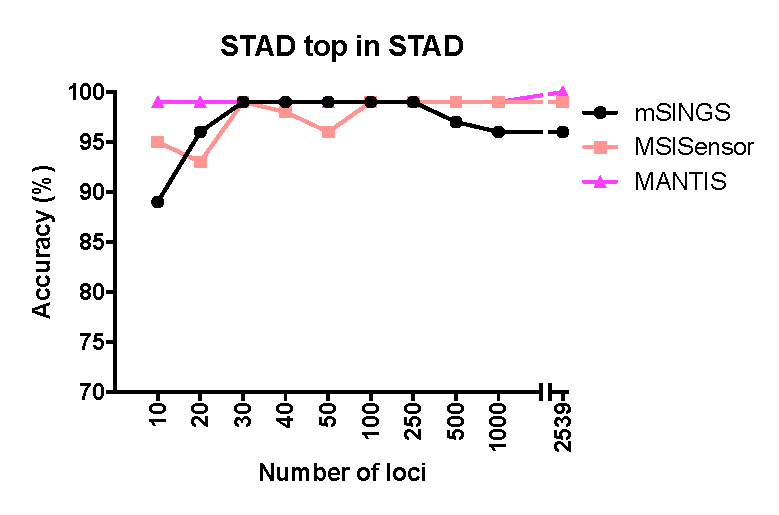
\includegraphics[width=\linewidth,keepaspectratio]{images/msilandscape/tool_performance_stad_loci_stad}
		\caption{}\label{fig:msilandscape:tool_performance_stad_loci_stad}
	\end{subfigure}
	\par
	\begin{subfigure}{0.33\textwidth}
		\includegraphics[width=\linewidth,keepaspectratio]{images/msilandscape/tool_performance_top_loci_coadread}
		\caption{}\label{fig:msilandscape:tool_performance_top_loci_coadread}
	\end{subfigure}%
	\hfill%
	\begin{subfigure}{0.33\textwidth}
		\includegraphics[width=\linewidth,keepaspectratio]{images/msilandscape/tool_performance_top_loci_ucec}
		\caption{}\label{fig:msilandscape:tool_performance_top_loci_ucec}
	\end{subfigure}%
	\hfill%
	\begin{subfigure}{0.33\textwidth}
		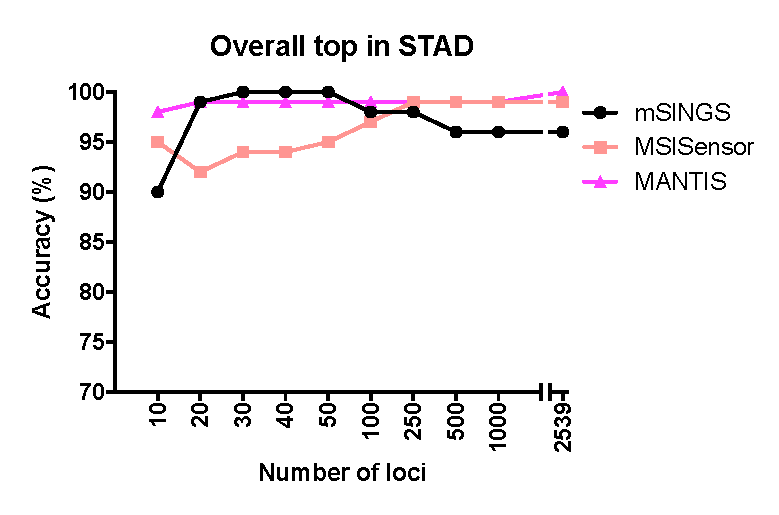
\includegraphics[width=\linewidth,keepaspectratio]{images/msilandscape/tool_performance_top_loci_stad}
		\caption{}\label{fig:msilandscape:tool_performance_top_loci_stad}
	\end{subfigure}
	\par
	\begin{subfigure}{0.33\textwidth}
		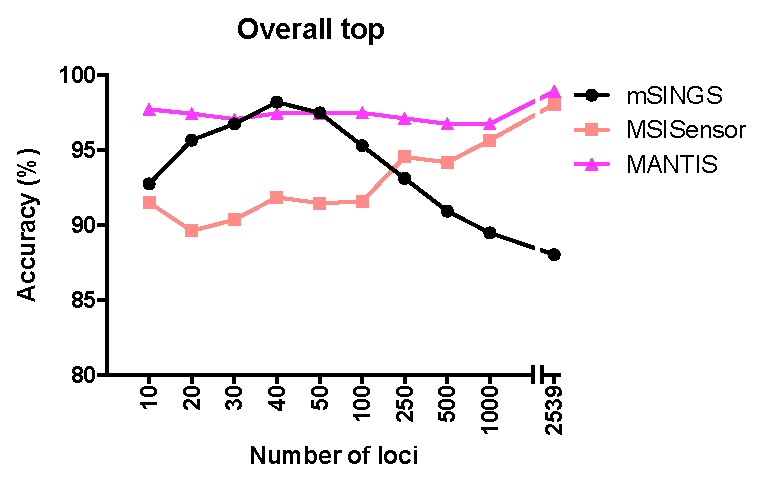
\includegraphics[width=\linewidth,keepaspectratio]{images/msilandscape/tool_performance_top_loci_all}
		\caption{}\label{fig:msilandscape:tool_performance_top_loci_all}
	\end{subfigure}
	\caption[Performance of mSINGS, MSISensor and MANTIS with their respective top-performing loci.]{The performance of mSINGS, MSISensor and MANTIS with their respective top-performing loci. For each tool, and within the COAD/READ, UCEC and STAD samples, the top-performing loci were determined, and the performance of each tool with these loci in each COAD/READ (\subref{fig:msilandscape:tool_performance_coadread_loci_coadread}), UCEC (\subref{fig:msilandscape:tool_performance_ucec_loci_ucec}) and STAD (\subref{fig:msilandscape:tool_performance_stad_loci_stad}) cohorts was evaluated with top tool- and cohort-specific loci (10-1000). In addition, the top-performing loci across all cohorts combined were determined, and performance of each tool with varying numbers of all-cohort top-performing loci in the COAD/READ (\subref{fig:msilandscape:tool_performance_top_loci_coadread}), UCEC (\subref{fig:msilandscape:tool_performance_top_loci_ucec}) and STAD (\subref{fig:msilandscape:tool_performance_top_loci_stad}) cohorts was determined. This analysis was also performed for all cohorts combined (\subref{fig:msilandscape:tool_performance_top_loci_all}). The results with 2,539 loci (without loci shortlisting) are included for reference.}
	\label{fig:msilandscape:tool_performance_top_loci}
\end{figure}

Previous studies have suggested that different MSI positive cancers may have specific microsatellite loci that are most commonly unstable \cite{faulkner2004,hempelmann2015}. For each MSI analysis tool, we sought to account for this by identifying the top-performing loci in each cancer type separately. Unlike in the analysis above, the 10, 20, 30, 40, 50, 100, 250, 500 and 1000 best-performing loci for each tool were determined for each COAD/READ, UCEC and STAD cohort separately (Supplemental File~S\thechapter{}.7). Each tool was then run over each cancer type, with respective top tool-specific and cancer-specific loci (Figure~\ref{fig:msilandscape:tool_performance_top_loci}a--c). Trends described in the previous analysis remained the same, with performance slightly higher throughout. However in UCEC at 40 loci, mSINGS performed better than MSISensor and MANTIS (98.0\% accuracy, vs.\ 89.9\% and 94.9\% respectively). Also, MANTIS and mSINGS both performed notably better (98.7\%) than MSISensor (83.6\%) when evaluating COAD/READ samples with 40 loci. The experiments show that the choice of loci being evaluated plays a part in tool performance. While an optimized target panel may allow all tools to perform well, MANTIS exhibits the most stable performance even without such optimizations, providing accurate performance using existing whole exome data.

\subsection{MSI landscape}
\label{ssec:msilandscape:landscape_results}
\begin{figure}[htp]
    \centering
    \begin{subfigure}{0.95\textwidth}
        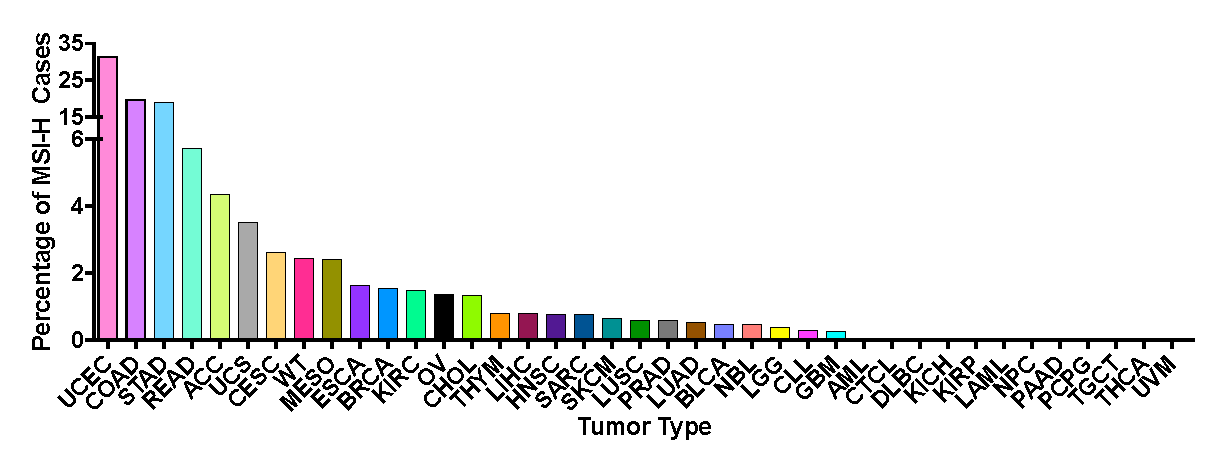
\includegraphics[width=\linewidth,keepaspectratio]{images/msilandscape/msi_landscape_bars}
        \caption{}\label{fig:msilandscape:msi_landscape_bars}
    \end{subfigure}
    
    \begin{subfigure}{0.95\textwidth}
        \includegraphics[width=\linewidth,keepaspectratio]{images/msilandscape/msi_landscape_dist}
        \caption{}\label{fig:msilandscape:msi_landscape_dist}
    \end{subfigure}
    \caption[Prevalence of MSI across 39 human cancer types.]{Prevalence of microsatellite instability (MSI) across 39 human cancer types. (\subref{fig:msilandscape:msi_landscape_bars}) MSI prevalence was detected across 39 tumor types. The total number of tumors and the percentage of cases called MSI-H in each cohort is listed in Table~\ref{table:msilandscape:landscape_summary}. (\subref{fig:msilandscape:msi_landscape_dist}) The relative level of instability, as measured by MANTIS score, is shown across all 39 tumor types. Note that for chronic lymphocytic leukemia (CLL), the listed MSI prevalence in panel (\subref{fig:msilandscape:msi_landscape_bars}) is out of 279 patients, and all 338 tumors are shown in panel (\subref{fig:msilandscape:msi_landscape_dist}), as some patients in this cohort had multiple tumors. MANTIS threshold cutoff of 0.4 is depicted with a dashed line. Cancer type abbreviations are listed in Appendix~\ref{app.cancerabbrev}.}
    \label{fig:msilandscape:msi_landscape}
\end{figure}
We analyzed paired whole exome sequencing data from 11,139 tumor-normal samples; 10,415 from the TCGA \cite{tcgageneric} database, 280 from the TARGET \cite{target} database, and 444 from other studies \cite{landau2015,choi2015,zheng2016,ong2012,chanon2013}, representing 39 distinct cancer types. MSI was detected in 27 of these 39 cancer types (Figure~\ref{fig:msilandscape:msi_landscape_bars}, Table~\ref{table:msilandscape:landscape_summary}, Supplemental File~S\thechapter{}.5). The disease-specific prevalence of MSI varied widely, from 31.4\% in endometrial carcinoma to 0.25\% in glioblastoma multiforme. MSI was not detected in 12 cancer types (Figure~\ref{fig:msilandscape:msi_landscape}). Of the 27 cancer types with MSI, 12 were found to have more than a single MSI-H tumor present, and MSI-H prevalence greater than 1\%. The relative level of instability, as measured by MANTIS score, varied substantially among cancer types that were MSI-H (Figure~\ref{fig:msilandscape:msi_landscape_dist}). In addition, we attempted to determine which specific microsatellite loci performed best across the greatest number of cancer types (Supplemental File~S\thechapter{}.8). Out of 2,530 loci, we identified 22 loci that, within at least five cohorts, had a MSI-H versus MSS difference score greater than 0.75 and were sufficiently covered by at least 50\% of samples in the cohort (Table~\ref{table:msilandscape:top_loci_landscape}). Only two loci assessed in the Bethesda \cite{boland1998} and Promega\textsuperscript\texttrademark{} \cite{bacher2004} MSI-PCR panels were included in our 2,530 loci, and neither of these were within the set of 22 top-performing loci. These results indicate a striking heterogeneity of microsatellite instability patterns across various cancer types.

\begin{figure}[ht]
    \centering
	\begin{subfigure}{0.33\textwidth}
		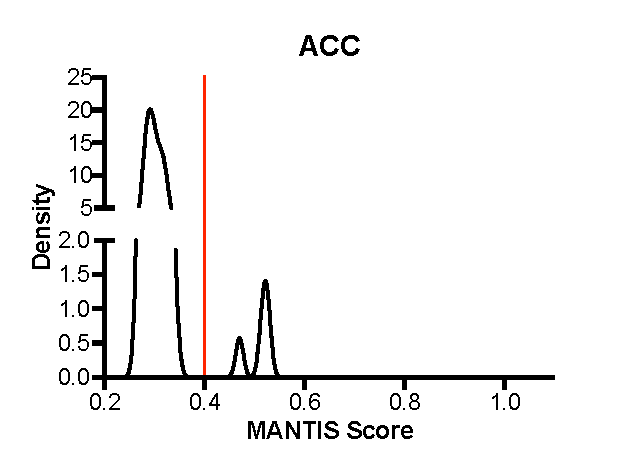
\includegraphics[width=\linewidth,keepaspectratio]{images/msilandscape/landscape_kd_acc}
		\caption{}\label{fig:msilandscape:landscape_kd_acc}
	\end{subfigure}%
	\hfill%
	\begin{subfigure}{0.33\textwidth}
		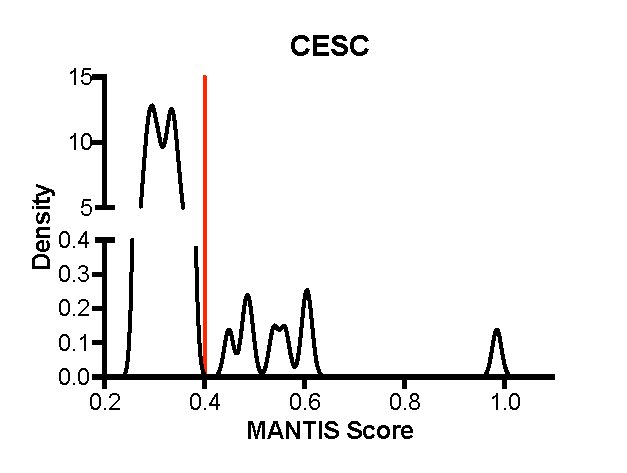
\includegraphics[width=\linewidth,keepaspectratio]{images/msilandscape/landscape_kd_cesc}
		\caption{}\label{fig:msilandscape:landscape_kd_cesc}
	\end{subfigure}%
	\hfill%
	\begin{subfigure}{0.33\textwidth}
		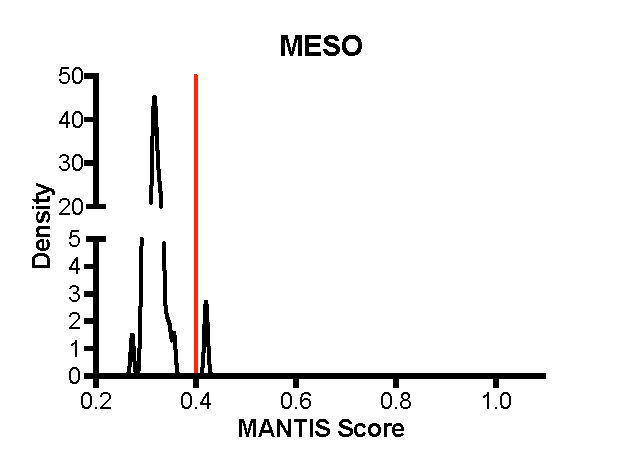
\includegraphics[width=\linewidth,keepaspectratio]{images/msilandscape/landscape_kd_meso}
		\caption{}\label{fig:msilandscape:landscape_kd_meso}
	\end{subfigure}
	\caption[Kernel density plots of MANTIS scores within ACC, CESC, and MESO.]{Kernel density plots of MANTIS scores within (\subref{fig:msilandscape:landscape_kd_acc}) adrenocortical carcinoma (ACC), (\subref{fig:msilandscape:landscape_kd_cesc}) cervical squamous cell carcinoma and endocervical adenocarcinoma (CESC), and (\subref{fig:msilandscape:landscape_kd_meso}) mesothelioma (MESO)\@. The dotted line denotes the average distance threshold of 0.4, used by MANTIS to differentiate microsatellite instability high from microsatellite stable tumors. ACC: $n = 92$, kernel bandwidth ($h$) $= 7.6 \times 10^{-3}$; CESC: $n = 305$, $h = 9.4 \times 10^{-3}$; MESO: $n = 83$, $h = 3.2 \times 10^{-3}$.}
	\label{fig:msilandscape:landscape_kd_acc_cesc_meso}
\end{figure}
All four disease types with the highest rates of MSI prevalence were Lynch syndrome-associated tumor types previously known to exhibit MSI: endometrial carcinoma, colon adenocarcinoma, gastric adenocarcinoma, and rectal adenocarcinoma. Consistent with previous studies, MSI was found to be more frequent in colon (19.7\%) than rectal (5.7\%) adenocarcinoma \cite{hause2016,phipps2013}. Of importance, MSI was detected in three cancer types that have not been previously well characterized, most notably adrenocortical carcinoma (ACC, 4.3\%), cervical squamous cell carcinoma and endocervical adenocarcinoma (CESC, 2.6\%), and mesothelioma (MESO, 2.4\%) (Figure~\ref{fig:msilandscape:msi_landscape_bars}). To further investigate MSI status classifications, kernel density estimation \cite{parzen1962,davis2011} was performed on the MANTIS scores for these tumor types. This indicated clear distinctions between samples MANTIS called MSI-H from samples called MSS (Figure~\ref{fig:msilandscape:landscape_kd_acc_cesc_meso}). Kernel density estimation was also performed on all other tumor types tested (Figure~\ref{fig:msilandscape:landscape_kd_others}).

\begin{figure}[htp]
    \centering
    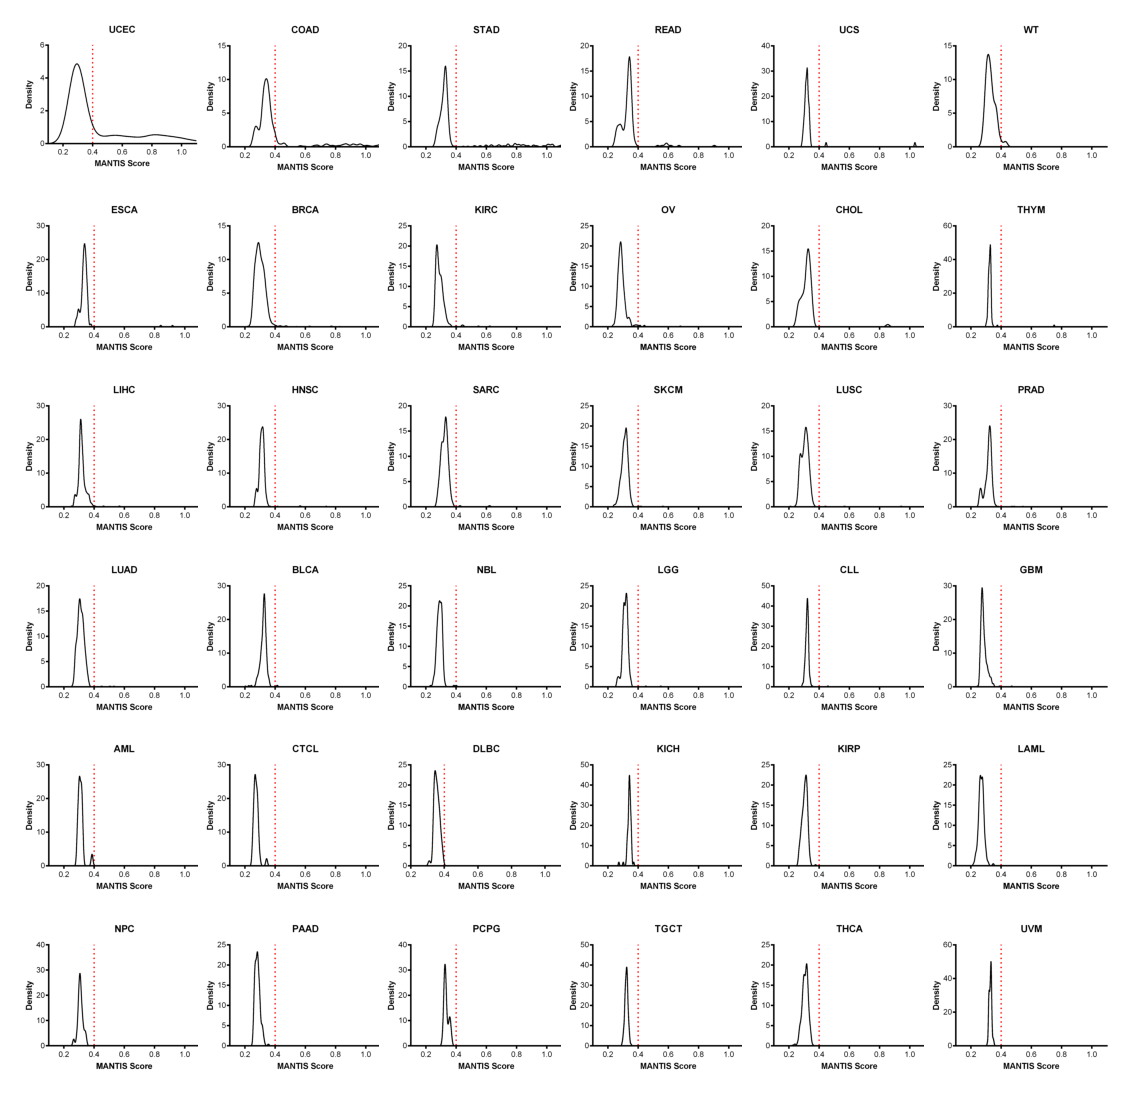
\includegraphics[width=0.98\linewidth,keepaspectratio]{images/msilandscape/landscape_kd_others}
    \caption[Kernel density plots of MANTIS scores within 36 cancer types.]{Kernel density plots of MANTIS scores within 36 cancer types. The dotted line denotes the average distance threshold of 0.4, used by MANTIS to differentiate microsatellite instability high from microsatellite stable tumors. UCEC: kernel bandwidth ($h$) = $4.89 \times 10^{-2}$. COAD: $h = 1.13 \times 10^{-2}$. STAD: $h = 7.59 \times 10^{-3}$. READ: $h = 9.16 \times 10^{-3}$. UCS: $h = 4.10 \times 10^{-3}$. WT: $h = 1.27 \times 10^{-2}$. ESCA: $h = 5.02 \times 10^{-3}$. BRCA: $h = 7.41 \times 10^{-3}$. KIRC: $h = 6.83 \times 10^{-3}$. OV: $h = 5.23 \times 10^{-3}$. CHOL: $h = 1.17 \times 10^{-2}$. THYM: $h = 3.08 \times 10^{-3}$. LIHC: $h = 4.42 \times 10^{-3}$. HNSC: $h = 4.25 \times 10^{-3}$. SARC: $h = 7.14 \times 10^{-3}$. SKCM: $h = 5.32 \times 10^{-3}$. LUSC: $h = 7.13 \times 10^{-3}$. PRAD: $h = 5.31 \times 10^{-3}$. BLCA: $h = 4.40 \times 10^{-3}$. CLL: $h = 2.64 \times 10^{-3}$. GBM: $h = 4.38 \times 10^{-3}$. AML: $h = 6.13 \times 10^{-3}$. CTCL: $h = 5.86 \times 10^{-3}$. DLBC: $h = 6.68 \times 10^{-3}$. KICH: $h = 3.34 \times 10^{-3}$. KIRP: $h = 5.16 \times 10^{-3}$. LAML: $h = 5.28 \times 10^{-3}$. NPC: $h = 6.09 \times 10^{-3}$. PAAD: $h = 5.36 \times 10^{-3}$. PCPG: $h = 5.04 \times 10^{-3}$. TGCT: $h = 3.40 \times 10^{-3}$. THCA: $h = 5.09 \times 10^{-3}$. UVM: $h = 3.06 \times 10^{-3}$.}
    \label{fig:msilandscape:landscape_kd_others}
\end{figure}

\subsection{Comparing TMB and signatures between MSI-H and MSS tumors}
\begin{figure}[ht]
    \centering
    \hfill%
	\begin{subfigure}{0.25\textwidth}
		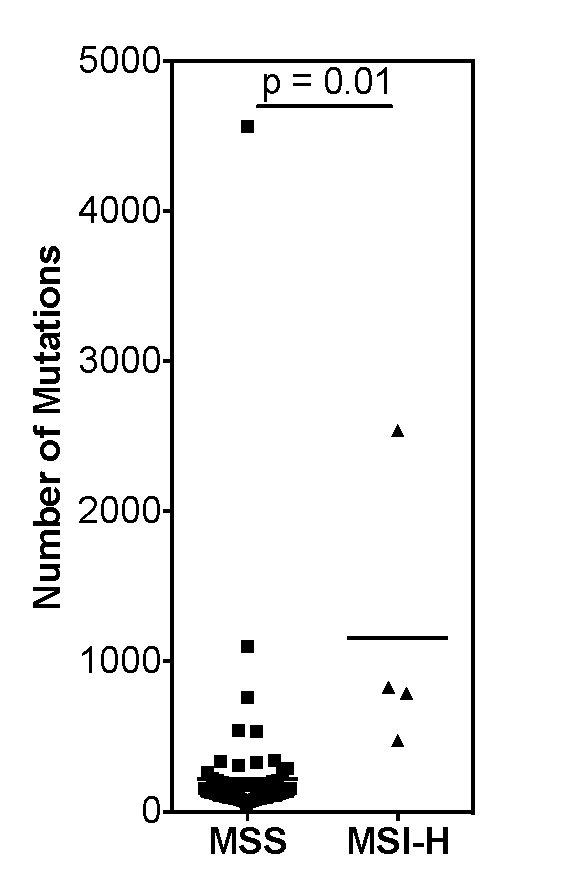
\includegraphics[width=\linewidth,keepaspectratio]{images/msilandscape/tmb_acc}
		\caption{}\label{fig:msilandscape:tmb_acc}
	\end{subfigure}%
	\hfill%
	\begin{subfigure}{0.25\textwidth}
		\includegraphics[width=\linewidth,keepaspectratio]{images/msilandscape/tmb_cesc}
		\caption{}\label{fig:msilandscape:tmb_cesc}
	\end{subfigure}%
	\hfill%
	\begin{subfigure}{0.25\textwidth}
		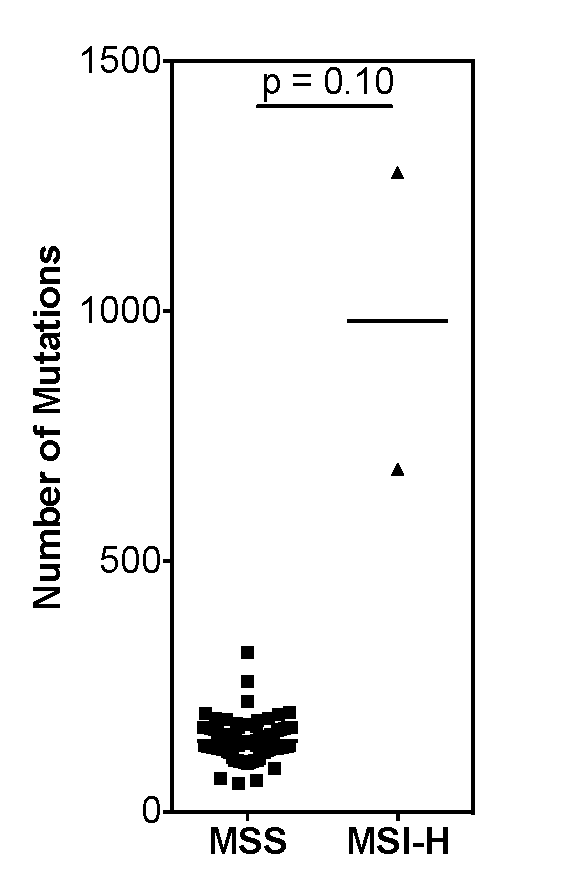
\includegraphics[width=\linewidth,keepaspectratio]{images/msilandscape/tmb_meso}
		\caption{}\label{fig:msilandscape:tmb_meso}
	\end{subfigure}%
	\hfill
	\caption[TMB correlates with MSI-H within ACC and CESC.]{Tumor mutational burden correlates with microsatellite instability high (MSI-H) status within adrenocortical carcinoma (ACC) and cervical squamous cell carcinoma and endocervical adenocarcinoma (CESC)\@. Mutational burden is listed for (\subref{fig:msilandscape:tmb_acc}) ACC, (\subref{fig:msilandscape:tmb_cesc}) CESC, and (\subref{fig:msilandscape:tmb_meso}) mesothelioma (MESO)\@. $P$ values were calculated using the Welch two-sample $t$-test of log-normalized absolute somatic mutation counts. Variant calling was performed by using MuTect (Section~\ref{ssec:msilandscape:variant_calling}), and all passing variants were included (nonsynonymous or synonymous).}
	\label{fig:msilandscape:tmb_acc_cesc_meso}
\end{figure}
Since Lynch syndrome-associated MSI-H tumors have been shown to have higher somatic tumor mutation burden (TMB) \cite{le2015,gatalica2016}, we performed further analysis to detect potential hypermutation in MSI-H ACC, CESC and MESO\@. Somatic variant calling was performed on whole exome samples from these four cancer types, and the mean absolute number of somatic mutations (both nonsynonymous and synonymous) was found to be increased among MSI-H versus MSS tumors within their own cohorts (Figure~\ref{fig:msilandscape:tmb_acc_cesc_meso}). In particular, an average of 1,157 somatic mutations were detected within MSI-H ACC samples, versus 216 within MSS ACC ($p = 0.01$). An average of 5,675 somatic mutations were detected within MSI-H CESC samples, versus 639 within MSS CESC ($p = 0.003$). Although statistical significance was not reached within MESO, MSI-H MESO tumors had, on average, nearly a seven-fold increase in TMB when compared to MSS MESO tumors (982 versus 142, $p = 0.10$). All $p$ values were calculated using Welch's two-sample $t$-test with log normalization. These results indicate that microsatellite instability in ACC and CESC is correlated with high TMB\@.

\begin{figure}[htp]
    \centering
    \includegraphics[width=0.98\linewidth,keepaspectratio]{images/msilandscape/sigs_acc_cesc_meso}
    \caption[Patterns of mutational signatures across cancers by microsatellite instability status.]{Patterns of mutational signatures (S) across cancers by microsatellite instability status. Cancers: (\textbf{A}) adrenocortical carcinoma (ACC), (\textbf{B}) cervical squamous cell carcinoma and endocervical adenocarcinoma (CESC), and (\textbf{C}) mesothelioma (MESO)\@. Mutational signatures were called using deconstructSigs from pooled variants from all MSI-H or MSS tumors within each cohort within ACC, CESC, and MESO\@. Unk., unknown.}
    \label{fig:msilandscape:sigs_acc_cesc_meso}
\end{figure}
To further investigate the observed somatic mutations in MSI-H versus MSS ACC, CESC, and MESO tumors, mutational signature analysis was performed using a set of 27 signatures introduced by Alexandrov \textit{et al} \cite{alexandrov2013}. A mutational signature defines a pattern of preferential somatic mutation types, and may be associated with a known biological process or cancer type. This analysis was first performed on pooled mutations among MSI-H or MSS samples within each of these three cancer cohorts (Figure~\ref{fig:msilandscape:sigs_acc_cesc_meso}). No clear pattern of signature differences was evident from this pooled analysis. Next, mutational signature analysis was performed for each individual case within these cohorts without pooling (Supplemental File~S\thechapter{}.9). Differences among signature prevalence in ACC, CESC, and MESO did not reach statistical significance. $P$ values were calculated using the two-sided Fisher exact test (using signature presence or absence), with Benjamini correction for multiple hypotheses.

\subsection{MMR pathway alterations}
\begin{table}[htbp]
    \centering
    {\small
    \begin{tabular}{lc:cccccc:c}
        & \textbf{Sample} & & & & & & \\
        \textbf{Variable} & \textbf{Count} & \textbf{\textit{MSH2}} & \textbf{\textit{MSH6}} & \textbf{\textit{MLH1}} & \textbf{\textit{PMS2}} & \textbf{\textit{EXO1}} & \textbf{\textit{POLE}} & \textbf{Any} \\
        \hline
        ACC & & & & & & & & \\
        \hphantom{---} MSS   & 88 & 1 & 1 & 0 & 1 & 0 & 1 & 4 \\
        \hphantom{---} MSI-H & 4 & 0 & 0 & 1 & 0 & 0 & 1 & 2 \\
        \hline
        CESC & & & & & & & & \\
        \hphantom{---} MSS   & 297 & 3 & 3 & 5 & 0 & 3 & 10 & 22 \\
        \hphantom{---} MSI-H & 8 & 0 & 1 & 3 & 1 & 1 & 2 & 6 \\
        \hline
        MESO & & & & & & & & \\
        \hphantom{---} MSS   & 81 & 0 & 1 & 0 & 0 & 0 & 1 & 2 \\
        \hphantom{---} MSI-H & 2 & 1 & 0 & 0 & 0 & 0 & 1 & 1 \\
        \hline
        ACC + CESC & & & & & & & & \\
        \hphantom{ACC }+ MESO & & & & & & & & \\
        \hphantom{---} MSS   & 466 & 4 & 5 & 5 & 1 & 3 & 12 & 28 \\
        \hphantom{---} MSI-H & 14 & 1 & 1 & 4 & 1 & 1 & 3 & 9
    \end{tabular}}
    \caption[Frequency of predicted deleterious MMR mutations in ACC, CESC, and MESO.]{Frequency of predicted deleterious MMR mutations in ACC, CESC, and MESO\@. Listed are the number of samples (MSS or MSI-H) with at least one predicted deleterious mutation in \textit{MSH2}, \textit{MSH6}, \textit{MLH1}, \textit{PMS2}, \textit{EXO1}, \textit{POLD1}, \textit{POLE}, or any of these genes (Any). Mutations were called using MuTect (Section~\ref{ssec:msilandscape:variant_calling}) and included in this table if the DANN pathogenicity score was $>0.96$.}
    \label{table:msilandscape:mmr_muts}
\end{table}
MSI-H Lynch syndrome-associated tumors are known to lack expression or function of at least one MMR protein. Therefore, we analyzed somatic mutations predicted to be deleterious (by DANN) in the mismatch repair genes \textit{MSH2}, \textit{MSH6}, \textit{MLH1}, \textit{PMS2} and \textit{EXO1}, and the proofreading DNA polymerases \textit{POLD1} and \textit{POLE}, among MSI-H and MSS samples within ACC, CESC, and MESO (Table~\ref{table:msilandscape:mmr_muts}), Supplemental File~S\thechapter{}.10). Though POLD1 and POLE are not considered MMR proteins, mutations in these genes have been shown to lead to somatic hypermutation \cite{tcgacoadread,johnson2015}. 64\% of MSI-H cases and 7\% of MSS cases within these cohorts were found to contain at least one predicted deleterious somatic mutation in at least one of these genes. However, given that these samples were sequenced with potentially different exome captures, and the increased mutational burden of MSI-H tumors, we could not determine the statistical significance of this finding.

\section{Discussion}
We have developed a new tool, MANTIS, for detecting MSI status using paired tumor-normal sequencing data. Unlike other tools, MANTIS analyzes the instability of a normal-tumor sample pair as an aggregate of loci instead of individual loci differences. The approach allows the tool to evaluate the general instability present in a tumor sample, using the data from the corresponding normal sample as an error-correcting baseline. Furthermore, by pooling the scores of all the loci and treating the average as the instability score, the evaluation benefits from the law of large numbers by reducing the impact that sequencing errors or poorly performing loci may have on the results.

We also analyzed the performance of MANTIS, mSINGS, and MSISensor with samples from six cancer types. Overall, MANTIS demonstrated high accuracy across a range of cancer types, and in many cases with restricted sets of well-performing loci. Prior tools have previously been applied to only one of two cancer types, endometrial (MSISensor) and colorectal (mSINGS)\@. With their recommended thresholds, mSINGS and MSISensor are less robust across a range of loci numbers than MANTIS\@. This appears to be due to the inclusion of poorly performing loci with low sensitivity in the full set of 2,539 loci. mSINGS and MSISensor call loci unstable or stable, and MANTIS calculates the instability at each locus. Suboptimal loci may be missed entirely by mSINGS and MSISensor, but still have some increased instability in MSI-H vs.\ MSS samples. Niu \textit{et al} recommend a relatively low threshold of 3.5 for MSISensor (vs.\ 20\% used by mSINGS and MSI-PCR)\@. This seems to effectively compensate for these poorly performing loci with a large panel, but greatly reduces the specificity of MSISensor when these loci are removed, as in the lists of top-performing loci. Conversely, the threshold of 0.2 (20\%) used by mSINGS is effective with a smaller panel of well-performing loci such as the mSINGS authors' panel MSIplus \cite{hempelmann2015}, but this threshold limits the sensitivity of mSINGS with a larger panel (Table~\ref{table:msilandscape:tool_accuracy}).

Results from UCEC were least concordant with the above trends. With the full set of 2,539 loci, MSISensor performed best, followed closely by MANTIS and distantly by mSINGS\@. This may potentially arise from differences in the microsatellite instability signatures between COAD/READ and UCEC, the existence of which is supported by previous findings \cite{alhopuro2012,kim2013}. A recent overview of microsatellite instability across multiple cancer types by Hause \textit{et al} further found significant variance in the number of unstable loci present between samples from different diseases \cite{hause2016}. Another potential explanation is that, because mSINGS was developed only with COAD/READ data and MSISensor only with UCEC data, these tools may be overfit to those cancer types. MANTIS, in contrast, was developed and tested using data from multiple cancer types, alleviating the potential overfitting issues that may occur when only including data from a single disease.

Like any NGS-based method, MANTIS performance depends on read coverage, a limitation not shared by MSI-PCR and IHC\@. Most current clinical guidelines for management of MSI positive tumors are based on a percentage of unstable loci. Current approaches for MSI detection (such as mSINGS, MSISensor, and MSI-PCR) use a discrete fraction of unstable loci to determine to make calls on the status of a sample, but MANTIS provides a continuously valued MSI score that may provide greater utility in determining the level of MSI present in a tumor. Findings by Hause \textit{et al} give further credence to this hypothesis, indicating that microsatellite instability may best be viewed as a scaled genotype rather than a simple binary positive or negative classification \cite{hause2016}.

We chose MANTIS, mSINGS, and MSISensor for this study since these three tools use NGS to directly assess microsatellite loci in DNA\@. Other NGS-based methods have been described that indirectly assess MSI through analysis of somatic mutations. MSIseq \cite{nihuang2015} employs machine learning classification techniques to correlate indels throughout repeat regions to MSI status. Stadler \textit{et al} \cite{stadler2016} describe a method utilizing a custom NGS assay, and correlating somatic missense and nonsense mutations in protein-coding regions with MSI status. Additionally, Lu \textit{et al} \cite{lu2013} describe an algorithm for determining MSI status from RNA-seq data. MSIseq was not included in this study as it is a classifier that only reports MSI-H vs.\ non-MSI-H, without a score or percentage, or information about the instability of particular loci. The Stadler \textit{et al} and Lu \textit{et al} methods were not included since they cannot be run with the same whole exome sequencing input data, requiring a custom deep-sequenced panel and RNA-seq data, respectively.

Currently, MMR and MSI status are determined in the clinical setting with IHC and MSI-PCR\@. Conventional multiplex MSI-PCR testing is reported to have 97\% sensitivity and 95\% specificity. IHC is reported to have 92.4\% sensitivity and 99.6\% specificity \cite{zhang2013}. MSI-PCR with the standard five Bethesda loci is well described for COAD/READ and UCEC \cite{armaghany2012}, but has been shown to perform less accurately in other diseases such as acute myeloid leukemia \cite{faulkner2004}, and may miss MSI in other tumor types. Consideration of only five loci renders conventional MSI-PCR highly susceptible to errors in processing or interpretation of any one locus, and adding additional loci increases cost. IHC is able to effectively determine the presence or absence of the mismatch repair proteins targeted. Unfortunately, IHC cannot detect loss-of-function mutations that do not affect the antigenicity of targeted proteins, or changes to MMR proteins not targeted \cite{shia2015}. Additionally, MSI-PCR and IHC require human interpretation, unlike computational NGS-based methods. Lastly, both MSI-PCR and IHC are clinical laboratory tests that consume fractions of patient tumor samples, unlike computational methods that could be multiplexed with other NGS assays for detecting somatic mutations.

As a tumor vs.\ normal algorithm, MANTIS avoids a time-consuming baseline generation step, eliminates potential baseline bias and allows processing of samples from different sequencing pipelines or tumor types without requiring a different baseline for each. Indeed, sequencing center bias may explain the discordance with mSINGS results from the 4 COAD/READ pairs sequenced at both BCM and BI (Table~\ref{table:msilandscape:coadread_by_site}). However, matched normal DNA is not always feasibly available for clinical laboratories that only sequence tumor samples, thus a tumor-only method such as mSINGS could reduce both sequencing time and cost to the patient.

The results of this study support several potential directions for future investigation. The accuracy of MANTIS with small numbers of loci suggests that MANTIS could be useful with a targeted sequencing panel designed for MSI testing in the clinic. With further investigation, incorporating MANTIS into clinical NGS pipelines may permit MSI testing on a large scale, and improve access to emerging therapies that exploit microsatellite instability in cancer. We have shown that MANTIS performs well in six cancer types; however it (along with other MSI tools) should be further evaluated in a wider variety of cancers. Of particular interest would be evaluation of MANTIS in neurologic, hematologic, pediatric and other malignancies, in which the landscape of MSI is considerably less well described than with COAD/READ and UCEC\@.

In this study, we have performed the largest-scale analysis of microsatellite instability in human cancer exomes as of July 2017, including 11,139 whole exome tumor-normal pairs from 39 cancer types. Compared to a study by Hause \textit{et al} \cite{hause2016}, we observed similar rates of MSI in 18 cancer types, and we further analyzed another 5,209 whole exome tumor-normal pairs from 21 additional cancer types. Additionally, we observed that MSI-H ACC and CESC tumors are significantly hypermutated, compared to MSS ACC and CESC tumors. We identified three cohorts with significant MSI prevalence that has not been previously well described. Of particular interest, we identified MSI in 4 of 92 (4.4\%) adrenocortical carcinoma cases. Previous studies of MSI in ACC have implicated Lynch syndrome as a risk factor for familial ACC \cite{challis2016,raymond2013} However, to our knowledge, NGS-based MSI analysis has not yet been applied to ACC\@.

MSI-H colorectal tumors have been previously shown to be exceptionally sensitive to therapy with PD-1 immune checkpoint inhibitors \cite{le2015}. Identification of MSI in novel tumor types may lead to an expanded role for immunotherapy, as well as a broader scope of clinical MSI testing \cite{dudley2016}. In addition, MSI is known to be prognostic within colorectal cancer \cite{kawakami2015}, which may apply in other cancer types as well. For instance, Hause \textit{et al} provide evidence that increasing MSI positively correlates with survival time. Clinical trials of immune checkpoint inhibitors are beginning or underway in ACC \cite{NCT02673333}, CESC \cite{NCT02635360}, and MESO \cite{NCT02784171,NCT02991482,NCT02707666,NCT02399371}, and a previous study of dendritic cell immunotherapy in ACC \cite{papewalis2006} demonstrated tumor marker but not clinical response. These studies may benefit from retrospective evaluation of MSI-H as a biomarker. Prospective expansion of clinical MSI testing to other cancer types may enlighten the prognostic and predictive value of MSI-H for non-colorectal cancers.

MMRd is well-recognized as the predominant cause of MSI within colorectal, endometrial and gastric cancers. Additionally, there have been anecdotal reports of ACC as a potential extracolonic manifestation of Lynch syndrome \cite{challis2016,raymond2013}. If future studies indicate that MSI in ACC, CESC, and/or MESO is indeed due to MMR deficiency, the findings of this study may implicate previously unappreciated cancer types as part of Lynch syndrome. Compared to germline alterations in MMR genes, somatic events are most often due to hypermethylation of CpG islands in the promoter region of \textit{MLH1} \cite{boland1998}. Further investigation is needed to elucidate other molecular mechanisms that can lead to MSI, as well as the downstream effects of MSI on tumor-specific biology. In addition, of the 9,569 tumors assessed in this study not within colorectal, endometrial, or gastric cancer, 77 (0.8\%) were MSI-H\@. Only 14 of these were within ACC, CESC, or MESO, compromising the statistical power of our mutational signature analysis. A larger cohort of MSI-H tumors would permit more comprehensive studies, including correlation with clinical data.

In summary, we have introduced a new MSI detection tool, MANTIS, and demonstrated its favorable performance compared to the previously published tools mSINGS and MSISensor. MANTIS exhibited the highest overall sensitivity and specificity within our test cohort comprising six cancer types, even with loci panels of varying size. Additionally, MANTIS also had the lowest resource consumption (\textless{}~1\% of the space and \textless{}~7\% of the memory required by mSINGS) and fastest running times (49.6\% and 8.7\% of the running times of MSISensor and mSINGS), respectively. We applied MANTIS to detect MSI in multiple additional cancer types including ACC, CESC, and MESO, indicating that MSI may affect non-Lynch syndrome tumor types. Within each cancer type having MSI, we identified which loci (among 2,530) were most predictive of overall tumor MSI status. With further analysis, these well-performing loci may form the basis of a targeted NGS panel for pan-cancer MSI detection. Additionally, we found that MSI-H tumors in ACC and CESC have higher mutational burden than MSS tumors of those types. Given our observations of a long tail of MSI-H tumors across multiple cancer types, we propose that patients presenting with these and other less common cancers undergo evaluation for MSI\@.

\section{List of Supplemental Files}
All supplemental files are available at \url{https://github.com/rbonneville/PhD-Dissertation/supplemental_files}.
\begin{enumerate}
    \renewcommand*{\labelenumi}{S\thechapter{}.\arabic{enumi}. }
    %mantis s1
    \item Summary of the TCGA (The Cancer Genome Atlas) and SU2C (Stand Up To Cancer) data used for main comparisons between mSINGS, MSISensor, and MANTIS\@.
    %mantis s2
    \item mSINGS, MSISensor and MANTIS scores for all 458 pairs used for testing and analysis of MSI calling tools. The results from the 24 pairs used for sequencing center comparison (Table~\ref{table:msilandscape:loci_number_perf}) are not included.
    %mantis s3
    \item Summary of the TCGA data used for tool comparisons by sequencing center.
    %mantis s4
    \item The performance of each locus assessed with mSINGS, MSISensor and MANTIS across the test cohorts, within COAD/READ, UCEC, STAD, and all three cancer types taken together. Coordinates are in hg19. Note that locus performance scores from MANTIS are not directly comparable to those from mSINGS or MSISensor, due to the different algorithms used by each.
	%landscape s1
	\item All cases analyzed for MSI to determine the landscape of MSI across 39 cancer types. For cases from TCGA or TARGET, listed file IDs are the GDC UUID correspond to the tumor and normal file. For all other cases, the file IDs are the SRA or EBI data accessions.
	%landscape s2
	\item Microsatellites analyzed using MANTIS in each landscape sample (except TCGA diffuse large B-cell lymphoma). Coordinates are in hg38.
    %mantis s5
    \item Performance of mSINGS, MSISensor and MANTIS in the COAD/READ, UCEC and STAD test cohorts, with each list of top loci (10, 20, 30, 40, 50, 100, 250, 500 or 1000, from COAD/READ, UCEC, STAD or overall, in COAD/READ, UCEC, STAD or overall, with mSINGS, MSISensor or MANTIS).
	%landscape s3
	\item The performance of each locus analyzed in each cancer type. Chronic lymphocytic leukemia (CLL) was excluded as many patients in this cohort had more than one tumor sample. Diffuse large B-cell lymphoma (DLBC) was excluded since MSI calling was performed with loci in hg19 (rather than hg38) coordinates. See ``About'' tab for field details.
	%landscape s4
	\item Mutational signatures called by deconstructSigs in each sample within ACC, CESC, and MESO.
	%landscape s5
	\item Predicted deleterious somatic mutations in the genes \textit{MSH2}, \textit{MSH6}, \textit{MLH1}, \textit{PMS2}, \textit{EXO1}, \textit{POLD1}, and \textit{POLE}, within ACC, CESC, and MESO. Mutations were called using MuTect (Section~\ref{ssec:msilandscape:variant_calling}), and included if DANN pathogenicity score $>0.96$.
\end{enumerate}

\section*{Acknowledgements}
We would like to acknowledge Pelotonia, the Prostate Cancer Foundation, the American Lung Association, the American Cancer Society, Stand Up To Cancer, the Ohio Supercomputer Center (OSC), and the Comprehensive Cancer Center (CCC) at the Ohio State University Wexner Medical Center. The results published here are in whole or part based upon data generated by The Cancer Genome Atlas managed by the NCI and NHGRI. Information about TCGA can be found at \url{http://cancergenome.nih.gov}. The results published here are in whole or part based upon data generated by the Therapeutically Applicable Research to Generate Effective Treatments (TARGET) initiative managed by the NCI. The data used for this analysis are available at dbGaP (accession phs000218.v17.p6). Information about TARGET can be found at \url{http://ocg.cancer.gov/programs/target}. The CLL sequencing data (dbGaP: phs000922.v1.p1) used in this work was supported by the National Human Genome Research Institute (NHGRI) Large Scale Sequencing Program, Grant U54 HG003067 to the Broad Institute (PI, Lander). We are grateful for administrative support from Jenny Badillo.

\chapter[Reconstruction of cholangiocarcinoma microevolution through rapid research autopsy]{Reconstruction of cholangiocarcinoma microevolution through rapid research autopsy\footnote{This chapter previously published as: Krook MA\cofirst, Bonneville R\cofirst, \textit{et al}. Tumor heterogeneity and acquired drug resistance in FGFR2 fusion-positive cholangiocarcinoma through rapid research autopsy. \textit{CSH Molecular Case Studies} 2019, 5:a004002.}}
\label{ch:240}

\section{Introduction}
Cholangiocarcinoma is an aggressive and deadly rare cancer arising from bile duct epithelial cells with a five-year overall survival rate of less than 2\% for advanced stage disease \cite{pdqchol2002,razumilava2014}. Most patients with cholangiocarcinoma present with metastatic unresectable cancer, thus precluding curative therapy \cite{razumilava2014,valle2010}. Given its poor prognosis and limited treatment options beyond first-line chemotherapy, development and optimization of novel therapies for cholangiocarcinoma is urgently needed.

The fibroblast growth factor receptor (FGFR) signaling pathway is aberrantly activated in approximately 20\% of cases of intrahepatic cholangiocarcinoma through various genomic alterations including point mutations, copy number amplifications, and gene fusions \cite{roychowdhury2011_ngs,wu2013}. Extending beyond cholangiocarcinoma, alterations in the FGFR signaling pathway have been reported in non-small cell lung carcinoma, endometrial cancer, and urothelial cancer \cite{krook2020}. Currently, several tyrosine kinase inhibitors, covalent and non-covalent, non-selective and selective FGFR inhibitors are being assessed clinically in patients with metastatic cancer and have shown early responses in those patients with metastatic FGFR-mutant cancers \cite{andre2013,angevin2013,gozgit2012,javle2018,paik2017,tabernero2015}. While genomic alterations in \textit{FGFR} correlated with initial clinical responses to FGFR inhibitors, multiple secondary mutations in \textit{FGFR} and other cellular signaling pathways have been identified in patients after treatment with FGFR inhibitors. Thus, elucidating the various acquired mechanisms of drug resistance to FGFR inhibitors will be critical for the development of new therapies to overcome resistance and improve the outcome of patients with FGFR-mutant cancers.

Tumor heterogeneity has been shown to negatively impact therapeutic response and contribute to treatment resistance in cancer patients, and thus it remains a major impediment to cancer treatment \cite{bedard2013,burrell2014,dexter1986,fisher2013,heppner1989}. Both genetic and epigenetic mechanisms within the tumor itself as well as changes in the tumor microenvironment can drive the development of tumor heterogeneity \cite{heng2009,junttila2013,meacham2013}. Genomic characterization of primary and recurrent/metastatic tumors from the same patient has further demonstrated spatial and temporal intrapatient tumor heterogeneity (ITH) \cite{bedard2013}. Recent studies have evaluated ITH and clonal evolution through next-generation sequencing (NGS) methods, demonstrating the critical role of these processes in recurrence and development of therapeutic resistance in urothelial carcinoma, renal cell carcinoma, and acute myeloid leukemia \cite{ding2012,faltas2016,gerlinger2012,gerlinger2014}. Studies like these, however, are limited in cholangiocarcinoma.

To date, the genomic landscape of cholangiocarcinoma has been largely characterized through tumor biopsies and surgical specimens and, therefore, may not accurately reflect the complex and heterogeneous nature of metastatic and drug-resistant disease \cite{farshidfar2017,jusakul2017,ruzzenente2016,zou2014}. Recently, Goyal \textit{et al} \cite{goyal2017} evaluated three patients with FGFR-fusion positive cholangiocarcinoma who received the FGFR inhibitor BGJ398. Targeted gene panel sequencing using the commercial Guardant360\textsuperscript\textregistered{} assay revealed an \textit{FGFR2} V564F gatekeeper mutation in plasma circulating tumor DNA (ctDNA) of all three patients and several additional FGFR2 mutations in two of the patients. One patient consented to rapid research autopsy and this enabled the procurement of multiple metastatic tumors for genomic profiling with the FoundationOne\textsuperscript\textregistered{} assay (315 gene panel) to study acquired drug resistance to the drug BGJ398. This study successfully demonstrated the role of acquired mutations in resistance to BGJ398. It also demonstrated heterogeneity at time of autopsy since 8 of 12 tumor samples assessed lacked a secondary mutation in \textit{FGFR2}. However, there are more than ten FGFR inhibitors in active drug development in clinical trials, and mechanisms of resistance for each of these drugs remain a significant gap in knowledge. Prior research on acquired resistance mutations in \textit{KIT}, \textit{ABL1}, and \textit{ALK} oncogenes with their respective kinase inhibitors, demonstrates that cross-resistance and sensitivity for secondary mutations varies widely, and therefore understanding resistance profiles for other FGFR inhibitors will be essential. Further, evaluating additional patients receiving other FGFR inhibitors with an expanded scope of whole exome (\textgreater{}~20,000 genes) will be critical to characterizing clonal heterogeneity and evolution with FGFR inhibitors.

In the current work, we present a patient with metastatic cholangiocarcinoma harboring a novel \textit{FGFR2-CLIP1} gene fusion who demonstrated a partial response followed by disease progression while on treatment with the FGFR-selective kinase inhibitor, INCB054828\footnote{INCB054828 has since been assigned the USAN generic name pemigatinib.}. Through rapid research autopsy of this patient and whole exome sequencing (WES) of his metastatic cancer, we identified four unique tumor subclones and elucidated their evolution from the normal ancestral cell. Furthermore, we identified a post-treatment secondary kinase mutation in \textit{FGFR2} present in a single metastatic tumor sample, and characterized its impact on sensitivity to a variety of FGFR inhibitors \textit{in vitro}. The results of our \textit{in vitro} drug sensitivity studies suggest that this mutation conferred resistance to INCB054828 in this patient and thus may have potential as a clinically useful biomarker of resistance. Importantly, characterizing tumor heterogeneity and the ability to detect clonal evolution in patients will facilitate approaches to prevent or overcome treatment resistance and disease recurrence.

\section{Materials and Methods}
\label{sec:240:methods}
\subsection{Research autopsy and patient samples}
\begin{figure}[htp]
    \begin{center}
        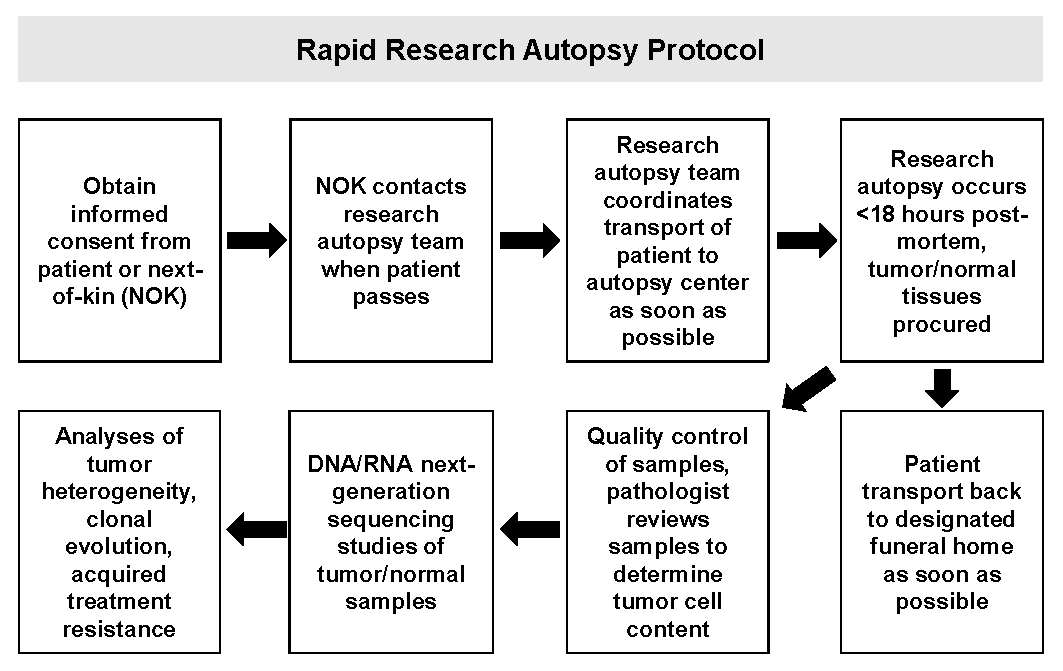
\includegraphics[width=0.85\textwidth,keepaspectratio]{images/240/autopsy_flowchart}
    \end{center}
    \caption{Overview of research autopsy protocol.}
    \label{fig:240:autopsy_flowchart}
\end{figure}
The patient consented to an IRB-approved study for high-throughput sequencing of tumor and normal specimens (OSU-13053, NCT02090530) at the James Cancer Hospital and The Ohio State University (Section~\ref{ssec:intro:heterogeneity_methods}). OSU-SpARKFuse, a targeted RNA based next generation sequencing assay to detect gene fusions, and a targeted DNA sequencing assay to detect single nucleotide variations were performed on tumor biopsy specimens as previously described \cite{samorodnitsky2015_ngs,reeser2017}. The patient also consented to a body donation study (Figure~\ref{fig:240:autopsy_flowchart}). Upon death of this patient, next of kin informed the research team, who arranged for transportation to the OSU Regional Autopsy Center and the autopsy was performed 8 hours post-mortem. Guided by radiographic scans, all visible malignant as well as adjacent normal tissues were collected and frozen in Optimal Cutting Temperature (OCT) compound. Following the autopsy, the patient was returned to the funeral home.

\subsection{Histology}
Freshly collected tumor biopsy and autopsy samples were immediately embedded and frozen in OCT compound (Thermo Fisher\textsuperscript\textregistered{}). Frozen sections were cut from tumor biopsy and autopsy samples at 5µm on a Leica\textsuperscript\texttrademark{} Cryostat CM1950 for H\&E staining. A board-certified pathologist reviewed representative slides for each tumor block for estimated tumor content.

\subsection{Whole exome sequencing}
Genomic DNA was extracted from frozen tumor biopsy samples and tumors collected during autopsy using the \mbox{QIAamp}\textsuperscript{\textregistered} DNA Mini Kit (Qiagen\textsuperscript{\textregistered}). The \mbox{QIAamp} DNA Mini Blood Kit (Qiagen) was used to extract genomic DNA from blood. Whole exome sequencing was performed as described below. Briefly, the KAPA HyperPrep\textsuperscript\texttrademark{} Kit (Roche\textsuperscript\texttrademark{}) was used for library preparation, and libraries were enriched using the xGen\textsuperscript\texttrademark{} Exome Research Panel v1.0 from Integrated DNA Technologies (IDT\textsuperscript\texttrademark{}). 2\texttimes{}150 bp paired-end sequencing was performed on an Illumina\textsuperscript\textregistered{} HiSeq\textsuperscript\textregistered{} 4000 at The Genomics Services Laboratory at Nationwide Children's Hospital (Columbus, Ohio).

\subsection{Sequence alignment and variant calling}
\label{ssec:240:alignment_variant_calling}
All bioinformatics analyses were performed using the Oakley supercomputer at the Ohio Supercomputer Center \cite{Oakley2012}. Alignment of whole exome sequencing data to the human genome version hg19 \cite{lander2001} was performed BWA \cite{bwa} version 0.7.14. Duplicate reads were removed with Picard \cite{Picard2019toolkit} version 2.3.0. Picard and GATK \cite{mckenna10} version 3.5 were used to perform quality recalibration and local realignment around indels. Single nucleotide variation (SNV) and indel calling were performed with VarScan2 \cite{varscan2} version 2.3.9. Raw somatic variant calls were filtered using bam-readcount \cite{bamreadcount} as follows:
\begin{table}[H]
	\centering
	\begin{tabular}{l|l}
		Filter                                   & Threshold  \\
		\hline
		$P$ (Fisher's exact test)                & $\le 0.05$ \\
		Average quality of alt-supporting reads  & $\ge 22$   \\
		Variant allele fraction                  & $\ge 6\%$  \\
		Average mutation distance to 3' read end & $\ge 0.24$ \\
		Mismatch rate in alt-supporting reads    & $\le 0.04$ \\
		Average sum of base quality mismatches   & $\le 100$
	\end{tabular}
	\label{table:240:somaticSNVfilter}
\end{table}
\noindent Germline SNVs (used for CNV calling) were filtered as follows:
\begin{table}[H]
	\centering
	\begin{tabular}{l|l}
		Filter                                   & Threshold  \\
		\hline
		$P$ (Fisher's exact test)                & $\le 0.1$  \\
		Average quality of alt-supporting reads  & $\ge 22$   \\
		Variant allele fraction                  & $\ge 6\%$  \\
		Average mutation distance to 3' read end & $\ge 0.24$ \\
		Mismatch rate in alt-supporting reads    & $\le 0.04$ \\
		Average sum of base quality mismatches   & $\le 100$
	\end{tabular}
\end{table}
\noindent To filter indels in difficult-to-call repetitive regions, RepeatFinder (packaged with MANTIS \cite{kautto17}) was used to generate a list of all regions in hg19 at least 4 bp in length that contained a 1 to 5-mer repeating sequence (Section~\ref{ssec:msilandscape:mantis}). Somatic indels were then filtered as follows:
\begin{table}[H]
	\centering
	\begin{tabular}{l|l}
		Filter                                   & Threshold  \\
		\hline
		$P$ (Fisher's exact test)                & $\le 0.05$ \\
		Variant allele fraction                  & $\ge 6\%$  \\
		Not in repetitive region & \\
	\end{tabular}
\end{table}

SNVs and indels were annotated using ANNOVAR \cite{annovar} (revision \#11f4bb, 2016-02-01) (Supplemental File~S\thechapter{}.1). Putative driver mutation analysis was performed with CRAVAT \cite{douville2013} version 5.2.4, using the CHASM \cite{carter2009}, algorithm version 3.1. Tumor mutational burden (TMB) was computed as the sum of all called somatic SNVs and indels within the capture region in each sample, divided by the size of the capture region (\textapprox{}38.9~Mb). Microsatellite instability (MSI) testing was performed with MANTIS \cite{kautto17} (Chapter~\ref{ch:msilandscape}) using the recommended threshold of 0.4 to call MSI and a set of 2,539 whole exome microsatellite loci (Section~\ref{ssec:msilandscape:loci_selection}). Mutational signatures were called with deconstructSigs \cite{rosenthal16} version 1.8.0 using the COSMIC Mutational Signatures set \cite{cosmic_ms}, exome2genome trinucleotide frequency correction, and otherwise default settings (Supplemental File~S\thechapter{}.2).

\subsection{Copy number variation analysis}
\label{ssec:240:cnv_methods}
Copy number variation (CNV) calling was performed using FALCON \cite{falcon} version 0.2, utilizing germline tumor and normal variants (Supplemental File~S\thechapter{}.3). The QC procedure provided with Canopy \cite{canopy} was employed to reduce false-positive segmentations, with default length and $\Delta$CN settings. For each sample, rdep (read depth ratio) was computed as the ratio of aligned reads in tumor vs.\ normal. FALCON was initially run with threshold 0.3. Resulting CNVs were manually curated to identify genomic regions with major copy number $>2$ or minor copy number $<0.5$ in at least one sample, and which spanned at least \textapprox{}25\% of a chromosome. For each curated region, a common pair of breakpoints was estimated across all tumors, and FALCON was re-run with threshold 0.2 and $\hat\tau_{chr}$ set to the nearest SNPs to each breakpoint in the chromosome (Supplemental File~S\thechapter{}.4). Matrices $\mathbf{W}_M$, $\mathbf{W}_m$, $\mathbf{\varepsilon}_M$, and $\mathbf{\varepsilon}_m$ (used for Canopy input) were obtained from FALCON output, and matrix $\mathbf{Y}$ was determined by calculating the overlap of mutations used for tree-building with curated CNV regions.

\subsection[Neighbor-joining trees]{Generation of neighbor-joining trees based on somatic variants}
\label{ssec:240:nj_methods}
To generate a sample-based phylogenetic tree, a distance matrix was first computed as follows:
\begin{equation}
    d_{ij} = \left| S_i \bigtriangleup S_j \right|
\end{equation}
where $\mathbf{D} \in \mathbb{Z}^{(N + 1) \times (N + 1)}$ is the distance matrix, $N$ is the number of samples, $S_i$ is the set of somatic SNVs called in sample $i \in 1 \twodots N$, and $\bigtriangleup$ is the set symmetric difference. The set of somatic SNVs in normal, corresponding to $i = N + 1$, is the empty set (by definition), therefore the distance between normal and any tumor collapses to the number of SNVs in that tumor. The tree was generated over $\mathbf{D}$ via neighbor-joining \cite{saitou1987} with RapidNJ \cite{simonsen08} version 2.3.2, and visualized using Interactive Tree of Life (iTOL) \cite{letunic16} version 4.2.3. Normal is regarded as the root of the tree.

\subsection{Subclonal inference}
\label{ssec:240:subclonal_inference}

\subsubsection{Mutation filtering}
\label{ssec:240:canopy_mut_filtering}
The reference read count, alternate allele count, and variant fractions of all nonsynonymous somatic variants called within each tumor sample were compiled. The set of somatic single nucleotide variants (SNVs) in each patient was then filtered for ultra-high-confidence SNVs. SNVs passing the following filters were classified as ultra-high-confidence:
\begin{itemize}
	\setlength\itemsep{-0.5em}
	\item{100\texttimes{} coverage in all tumor samples}
	\item{$\ge 20$ alt-supporting reads in at least one tumor sample}
	\item{Mutation on an autosome}
	\item{DANN \cite{quang2015} mutational impact prediction $\ge 0.96$}
\end{itemize}

\subsubsection{Tree construction}
\label{ssec:240:canopy_tree}
Canopy \cite{canopy} was then run with an in-house parallelized version of \texttt{sample.cluster} mode with cluster number from 2 to 9, 10 MCMC clustering runs, $\tau_{K+1} = 0.05$, number potential subclones from 3 to 9, 50 chains per subclone number, burnin 100, thinning parameter 5, simulation runs from 20000 to 50000, and writeskip 200. As FALCON does not generate standard deviations for regions with identical major and minor copy number, and Canopy does not support sparse $\varepsilon_M$ or $\varepsilon_m$ matrices, the Frobenius norm of non-NA values of the $\varepsilon_M$ and $\varepsilon_m$ matrices was used for Canopy. 

\begin{figure}[htp]
	\centering
	\includegraphics[width=0.7\linewidth,keepaspectratio]{images/240/bic}
	\caption[BIC scores of subclonal models with 3--9 clonal populations.]{BIC score of subclonal models with 3--9 clonal populations. Models with 3 to 9 clonal populations were tested by Canopy. A five-population model was selected (BIC = -40,684.12), as higher-complexity models did not yield substantially higher BIC (maximal BIC = -40,301.74 with 9 clonal populations). Note that germline is considered a clonal population by Canopy, therefore the selected model contains four tumor subclones.}
	\label{fig:240:bic}
\end{figure}
Canopy computes a Bayesian Information Criterion \cite{schwarz1978} (BIC) score for each potential number of subclones, which was used to determine the number of subclones that best represents the data. A 4-clone model was selected since models with additional subclones only yielded marginal increases in BIC (Figure~\ref{fig:240:bic}). Note that Canopy estimates its normal cell fractions based on variant fractions and CNV data, and reported purities can differ from pathologist estimates, likely because different sections of the tumor blocks were sequenced than were reviewed by the pathologist (Supplemental File~S\thechapter{}.5).

\subsubsection[Post hoc mutation assignment]{\textit{Post hoc} mutation assignment}
\label{ssec:240:tree_assignment}
Afterwards, the remaining somatic SNVs (not used for Canopy tree building) and indels were retroactively assigned to the resulting tree using a maximal likelihood model. From Canopy, we have a phylogenetic tree $G = (V, E)$, in which $v_1$ corresponds to the patient's germline and other vertices correspond to tumor subclones. Define $N$ as the number of tumor samples. For an arbitrary somatic mutation $m$, define $\vec{r} \in \mathbb{Z}^N$ as the number of alternate-supporting reads for $m$ in each sample, $\vec{x} \in \mathbb{Z}^N$ as the coverage of the variant position in each sample, and $\vec{p} \in \mathbb{R}^N$, a vector of expected variant fractions in each sample (derived from the tree as shown below). Given known $\vec{x}$ and $\vec{p}$, and modeling alternative read depth as jointly binomial across tumor samples, the probability and log-likelihood that $m$ is within an edge $e \in E$ can be computed as follows:
\begin{subequations}
    \begin{equation}
        P(\vec{r} | \vec{x}, \vec{p}) = \prod_{i=1}^{N} \dbinom{x_i}{r_i} p_i^{r_i} (1 - p_i)^{(x_i - r_i)}
    \end{equation}
    \begin{align}
        \mathcal{L}(m \in e) &= \ln\left(P(\vec{r} | \vec{x}, \vec{p})\right) \nonumber \\
        &= \sum_{i=1}^N \left( \sum_{j=r_i + 1}^{x_i} \ln(j) - \sum_{j=1}^{x_i - r_i} \ln(j) + r_i \ln(p_i) + (x_i - r_i) \ln(1 - p_i) \right)
    \end{align}
\end{subequations}

To compute $\vec{p}$, we utilize the phylogenic tree and clonal fractions reported by Canopy, along with its per-subclone major and minor copy number estimates. We construct a matrix $\mathbf{T} \in \{0, 1\}^{|E| \times |V|}$ as follows:
\begin{equation}
    T_{e, v} = \begin{cases}
        1 & \text{if the path from } v_1 \text{ to vertex } v \text{ contains edge } e \\
        0 & \text{otherwise}
    \end{cases} \qquad e \in E, v \in V
\end{equation}

From CNV calling, we have $T$, the number of CNV regions. We also have from Canopy the clonal matrix $\mathbf{P} \in \mathbb{R}^{|V| \times N}$, in which each column corresponds to the proportions of the respective subclone (or germline) in each tumor sample, $\tilde{\mathbf{C}}^M \in \mathbb{Z}^{T \times |V|}$ as the per-subclone major copy number matrix, and $\tilde{\mathbf{C}}^m \in \mathbb{Z}^{T \times |V|}$ as the per-subclone minor copy number matrix. Any zero values within each column of $\mathbf{P}$ were set to $0.0005$, and remaining entries reduced equally to maintain the constraint that each column sums to 1. This is first used to compute $\mathbf{A} \in \mathbb{R}^{T \times N}$, the total copy number of each CNV-affected region in each sample (independent of any specific mutation), as follows:
\begin{equation}
    \mathbf{A} = (\tilde{\mathbf{C}}^M + \tilde{\mathbf{C}}^m)\mathbf{P}
\end{equation}

Next, assume without loss of generality that mutation $m$ is within edge $e$. If $m$ is within a CNV $t$, we know from Canopy the edge $y \in E$ that contains $t$. We can calculate the copy number of $m$ in each subclone, $\vec{b} \in \mathbb{Z}^{|V|}$, as follows:
\begin{subequations}
    \begin{equation}
        \mathbf{C} = \begin{cases}
            \tilde{\mathbf{C}}_{t*}^M & m \text{ is on major allele of CNV } t \text{, and } y \text{ is further from } v_1 \text{ than } e \\
            \tilde{\mathbf{C}}_{t*}^m & m \text{ is on minor allele of CNV } t \text{, and } y \text{ is further from } v_1 \text{ than } e \\
            \{1\}^K & m \text{ is not within any CNV, or } e \text{ is further from } v_1 \text{ than } y
        \end{cases}
    \end{equation}
    \begin{equation}
        \vec{b} = (\mathbf{T}_{e*} \circ \mathbf{C})\mtpose
    \end{equation}
\end{subequations}
where $\circ$ is the Hadamard product of matrices. This permits calculation of the expected copy number of $m$ in each sample $\vec{s} \in \mathbb{R}^N$, provided that $m \in$ an edge $e$ and $m$ is on a major or minor allele, as follows:
\begin{equation}
    \vec{s} = \mathbf{P}\mtpose \vec{b}
\end{equation}
Computation of $\vec{p}$ for mutation $m$ is now straightforward:
\begin{equation*}
    \vec{a} = \begin{cases}
        \mathbf{A}_{t*}\mtpose & m \text{ is within CNV } t \\
        \{2\}^N & m \text{ is not within an CNV, and is on an autosome or chrX in a female} \\
        \{1\}^N & m \text{ is on chrX or chrY in a male}
    \end{cases}
\end{equation*}
\begin{equation}
    p_i = \frac{s_i}{a_i} \qquad i = 1 \twodots N
\end{equation}

To perform the assignment of mutation $m$, $\mathcal{L}(m \in e)$ is computed for all edges $e \in E$. If $m$ is within a CNV region and the candidate edge is before the CNV, its possibilities of being on the major or minor allele are both considered. If the candidate edge is after the CNV, only the possibility of it occurring on one copy of the allele is considered, utilizing the simplifying assumptions (also made by Canopy) that each somatic mutation occurs only once and no back-mutations occur. If the candidate edge contains the CNV, all three above possibilities (major\slash{}minor\slash{}after) must be considered. To avoid numerical errors, if $p_i = 0$ and $r_i \neq 0$ for a candidate assignment in any sample, that candidate assignment is discarded. The edge with highest log-likelihood is selected, with ties (such as can occur with deletions or on a different edge than a CNV) broken in favor of the edge furthest from the root node. This approach was implemented and run using Python 2.7.1, using scipy \cite{2020SciPy-NMeth} 0.10.1.

\subsubsection{Mutational ordering}
\label{ssec:240:mutational_ordering}
Mutations within each branch of the tree were temporally ordered using a Bradley-Terry model \cite{terry52}. Given a phylogenetic tree $G = (V, E)$ from Canopy and \textit{post hoc} tree assignment, we have a set of mutations $M_e$ for each edge $e \in E$. Define $\vaf_i(m)$ as the variant fraction (VF) of mutation $m$ in tumor sample $i \in 1..S$, where $S$ is the set of tumor samples used to build $G$.

We regard each pair of variants $m_1, m_2 \in M_e$ in each tree edge and sample as a contest, with the \emph{score} of $m_1$ vs.\ $m_2$ in sample $i$ as follows:
\begin{equation}
	w_i(v_1, v_2) = 
	\begin{cases}
		1 & \vaf_i(m_1) > \vaf_i(m_2) \\
		0 & \vaf_i(m_1) < \vaf_i(m_2) \\
		0.5 & \vaf_i(m_1) = \vaf_i(m_2)
	\end{cases}
\end{equation}
Summing all pairwise scores from all samples yields the wins matrix $\mathbf{V} \in \mathbb{R}^{|M_e| \times |M_e|}$:
\begin{equation}
	V_{jk} = \begin{cases} \sum_{i=1}^S w_i(m_j, m_k) & j \ne k \\ 0 & j = k \end{cases} \qquad j, k \in 1..|M_e|
\end{equation}

The Bradley-Terry model yields \emph{abilities} $\pi_m$ for each mutation, such that:
\begin{equation}
	P(m_1 \text{ occurred before } m_2) = \frac{\pi_1}{\pi_1 + \pi_2}
\end{equation}
where $\pi_1$ and $\pi_2$ are the abilities of mutations $m_1$ and $m_2$. The maximum \textit{a priori} estimate of abilities \cite{btbayesian} was computed using the R package \texttt{BradleyTerryScalable} \cite{btscalable} with $a = 1.1$. Note that ability scores denote confidence in ordering, not the time intervals between acquisition of mutations. This analysis was performed independently for each edge of the clonal phylogeny tree, utilizing both mutations supplied to Canopy and those retroactively assigned to the tree.

\subsection{Droplet digital PCR and analysis}
Isolated genomic DNA was amplified using a custom designed probe for the \textit{FGFR2} N549H point mutation (PrimePCR ddPCR Mutation Assay, Bio-Rad\textsuperscript\textregistered{}) and the ddPCR Supermix for Probes (Bio-Rad). The reaction mixture consisted of 250 ng of DNA template (8~\textmu{}L), 10~\textmu{}L of ddPCR Supermix for Probes (Bio-Rad) and 2~\textmu{}L of the primer/probe mixture. Droplets were generated using the QX200 Droplet Generator (Bio-Rad) and then transferred to a 96-well plate (Eppendorf\textsuperscript\textregistered{}) for PCR amplification with the following conditions: 5 minutes at 95~\textdegree{}C, 40 cycles of 94~\textdegree{}C for 30 seconds, 55~\textdegree{}C for 1 minute followed by 98~\textdegree{}C for 10 minutes (ramp rate 2~\textdegree{}C/second). Droplets were analyzed with the QX200 Droplet Reader (Bio-Rad) for fluorescent measurement of FAM and HEX probes. Gating was performed based on positive and negative controls, and mutant populations were identified. All reactions were run in duplicate. The ddPCR data were analyzed with QuantaSoft analysis software (Bio-Rad) to obtain fractional abundance of the mutant DNA alleles in the wild-type (WT)/normal background.

\subsection{cDNA plasmid generation, lentivirus production and transduction}
\begin{figure}[htp]
	\centering
	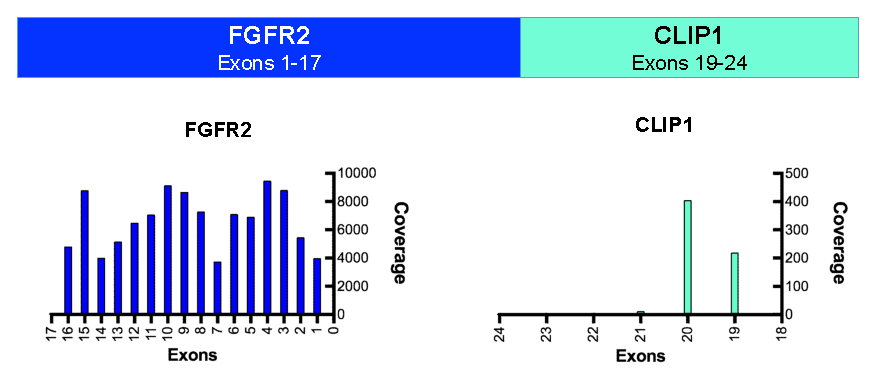
\includegraphics[width=0.8\linewidth,keepaspectratio]{images/240/fusion_coverage}
	\caption[RNA-seq coverage of novel FGFR2-CLIP1 fusion.]{RNA-seq coverage of novel FGFR2-CLIP1 fusion. A novel fusion containing exons 1--17 of \textit{FGFR2} and exons 19--24 of \textit{CLIP1} was detected in a patient with cholangiocarcinoma.}
	\label{fig:240:fusion_coverage}
\end{figure}
The \textit{FGFR2-CLIP1} fusion was produced and cloned into the pLVX-IRES-Puro vector (Clontech) by GenScript\textsuperscript\textregistered{}, containing exons 1--17 of \textit{FGFR2} and exons 19--24 of \textit{CLIP1} (Figure~\ref{fig:240:fusion_coverage}). Using site directed mutagenesis, the \textit{FGFR2} N549H mutation was introduced into the fusion by GenScript. NIH3T3 cells were stably transduced with either empty, \textit{FGFR2-CLIP1} or \textit{FGFR2-CLIP1} N549H lentiviral vectors. Cells were selected in puromycin (1~\textmu{}g/mL; Sigma-Aldrich\textsuperscript\textregistered{}) for 72 hours prior to their use in downstream experiments.

\subsection{RNA isolation, RT-PCR and Sanger sequencing}
\begin{table}[H]
    {\small
	\begin{center}
		\begin{tabular}{cccc}
			 & & & \textbf{Product} \\
			\textbf{Target} & \textbf{Forward} & \textbf{Reverse} & \textbf{Size (bp)} \\
			\hline
			FGFR2-CLIP1 & 5'--\texttt{CAGAGACCAACGTTCAAGCA}--3' & 5'--\texttt{CGGCATCCTTTTCTGTGAGT}--3' & 214 \\
			N549H & 5'--\texttt{GTGGCCGTGAAGATGTTGAA}--3' & 5'--\texttt{AGGTATTCTCGGAGGTTGCC}--3' & 188
		\end{tabular}
	\end{center}}
	\vspace{-0.3cm}
	\caption[Primer sequences.]{Primer sequences used for PCR and Sanger sequencing to confirm the presence of either the fusion or the mutation.}
	\label{table:240:primer_seqs}
\end{table}
RNA was isolated from cell lines, and cDNA was synthesized using The Quick-RNA Mini Prep Kit (Zymo Research\textsuperscript\texttrademark{}) and the iScript cDNA Synthesis Kit (Bio-Rad), respectively. cDNA was subsequently PCR amplified with \textit{FGFR2-CLIP1} and \textit{FGFR2} N549H fusion specific primers (IDT)\@. Primer sequences are listed in Table~\ref{table:240:primer_seqs}. The Invitrogen PureLink Quick PCR Purification Kit (Thermo Fisher) was used to purify amplified PCR product and samples were then Sanger sequenced (The Ohio State University Comprehensive Cancer Center Genomics Shared Resource, Columbus, OH).

\subsection{Cell culture}
NIH3T3 and HEK293T cell lines were purchased from American Type Culture Collection (ATCC\textsuperscript\textregistered{}) and cultured in a humidified incubator at 37~\textdegree{}C and 5\%~CO\textsubscript{2}. Cells were cultured according to ATCC recommended protocols. All cell lines were routinely subjected to short tandem repeat profiling to confirm identities and \textit{Mycoplasma} testing using the e-Myco Plus Mycoplasma PCR Detection Kit (Bulldog Bio\textsuperscript\texttrademark{}).

\subsection{Western blotting}
Western blot assays were carried out using established protocols and probed with the following antibodies: phospho-Akt (Ser473) 1:1000 (Cell Signaling Technology\textsuperscript\textregistered{} 9271), Total Akt 1:1000 (Cell Signaling 9272), phospho-MEK1/2 1:5000 (Cell Signaling 9154), Total MEK1/2 1:5000 (Cell Signaling 9122), p44/42 MAPK (Erk1/2) 1:5000 (Cell Signaling 9101), Total MAPK 1:5000 (Cell Signaling 9102), phospho-FGF Receptor (Tyr653/654) 1:500 (Cell Signaling 3471), FGF Receptor 2 (D4L2V) 1:500 (Cell Signaling 23328),  phospho-PLC$\gamma$1 (Tyr783) 1:1000 (Cell Signaling 14008), PLC$\gamma$1 (D9H10) 1:1000 (Cell Signaling 5690), phospho-FRS2\nobreakdash-$\alpha$ (Tyr196) 1:1000 (Cell Signaling 3864), FRS2 1:1000 (Abcam\textsuperscript\textregistered{} 10425), phospho-PI3 Kinase p85 (Tyr458)/p55 (Tyr199) 1:1000 (Cell Signaling 4228), PI3 Kinase p85 (19H8) 1:1000 (Cell Signaling 4257), $\beta$-actin 1:10000 (Cell Signaling 4967).

\subsection{Drug sensitivity assays}
NIH3T3 Empty, \textit{FGFR2-CLIP1}, and \textit{FGFR2-CLIP1} N549H cells were plated at a density of 10,000 cells per well in 96-well plates. Cells were treated for 72 hours with either INCB054828 (Incyte\textsuperscript\textregistered{}), BGJ398 (Cayman Chemical\textsuperscript\textregistered{}), JNJ-42756493 (Cayman Chemical), AZD-4547 (Cayman Chemical), ponatinib (Cayman Chemical), or dovitinib (Cayman Chemical) ranging from 0.01 to 5000~nM\@. Quantification of viable cells was assessed using an MTS/PMS colorimetric assay. IC\textsubscript{50} values were calculated in Prism (GraphPad) using a 4-parameter dose-response model.

\section{Results}
\subsection{Clinical course}

\begin{figure}[htp]
    \centering
    \begin{subfigure}{0.8\textwidth}
        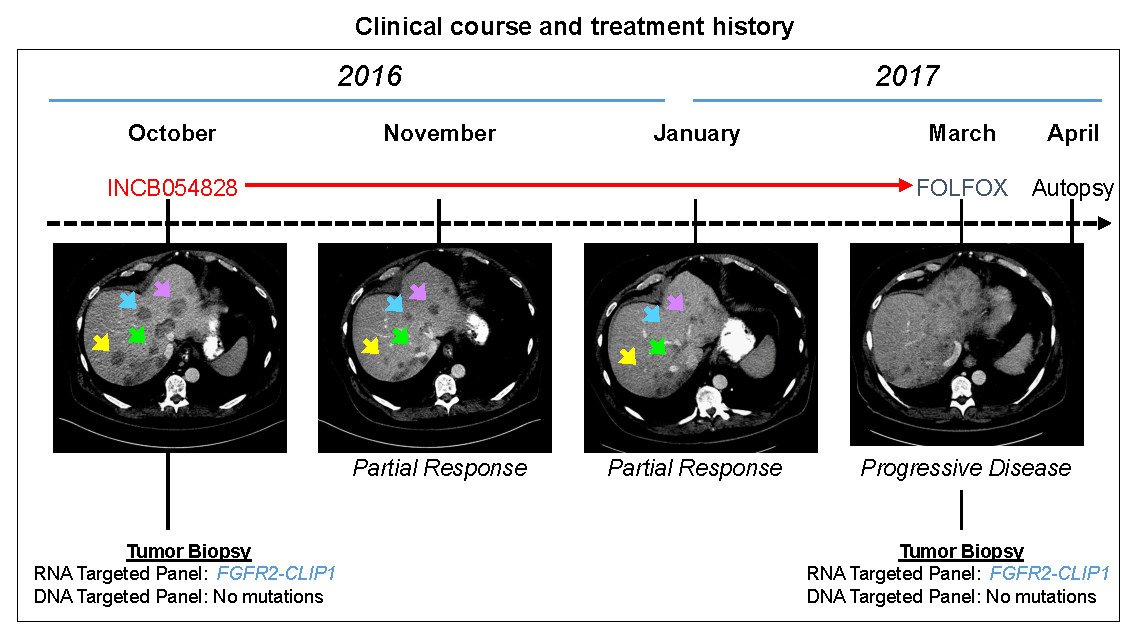
\includegraphics[width=\textwidth,keepaspectratio]{images/240/clinical_course}
        \caption{}\label{fig:240:clinical_course}
    \end{subfigure}\par
    \begin{subfigure}{0.8\textwidth}
        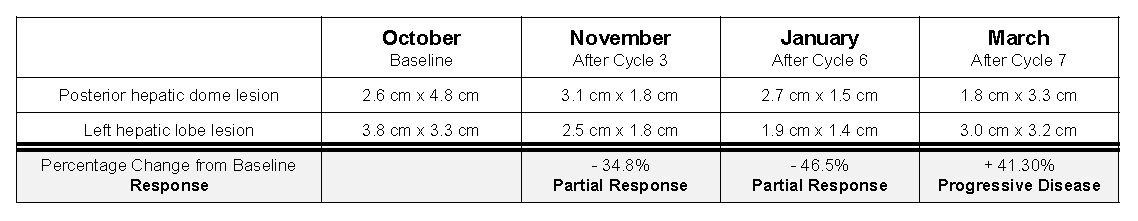
\includegraphics[width=\textwidth,keepaspectratio]{images/240/recist}
        \caption{}\label{fig:240:recist}
    \end{subfigure}\par
    \begin{subfigure}{0.8\textwidth}
        \includegraphics[width=\textwidth,keepaspectratio]{images/240/fusion_schematic}
        \caption{}\label{fig:240:fusion_schematic}
    \end{subfigure}
    \vspace{-0.2cm}
    \caption[Description of a cholangiocarcinoma patient harboring an FGFR2-CLIP1 fusion.]{Description of a patient with metastatic cholangiocarcinoma harboring an \textit{FGFR2-CLIP1} fusion. (\subref{fig:240:clinical_course}) Clinical course of this patient with selected CT scans. (\subref{fig:240:recist}) Table summarizing two target lesions (posterior hepatic dome lesion and left hepatic lobe lesion) that were tracked throughout the treatment course and had a 24.8\% and 46.5\% reduction from baseline after cycles 3 and 6, respectively. (\subref{fig:240:fusion_schematic}) Schematic of the \textit{FGFR2-CLIP1} fusion involving exons 1--16 of \textit{FGFR2} and exons 19--24 of \textit{CLIP1}. Chromatogram traces from Sanger sequencing of the tumor biopsy confirmed the presence of the fusion. Red dashed line indicates breakpoint within sequence.}
    \label{fig:240:clinical_desc}
\end{figure}
A 59-year old male presented clinically with abdominal pain and fullness in the fall of 2015 (Figure~\ref{fig:240:clinical_course}). Abdominal CT and MRI scans revealed two small but suspicious appearing lesions in the liver. He underwent biopsy of one liver lesion and pathology demonstrated poorly differentiated adenocarcinoma with focal neuroendocrine differentiation (CK7\textsuperscript{+}, CDX2\textsuperscript{+}, synaptophysin\slash{}chromogranin\textsuperscript{+}, CK20\textsuperscript{-}, TTF1\textsuperscript{-}, napsin\textsuperscript{-}) consistent with pancreatic or biliary origin. A PET-CT scan showed localized cancer in the right hepatic lobe, and he subsequently underwent surgical resection with clear margins and no lymph node involvement. Surgical pathology confirmed intrahepatic cholangiocarcinoma, which was staged as T2aN0. He received no adjuvant therapy post-surgery. Five months later, in April 2016, surveillance MRI showed emergence of new hepatic tumors, prompting palliative treatment with gemcitabine and cisplatin (Gem/Cis). Gemcitabine (1000~mg/m\textsuperscript{2}) and cisplatin (25/m\textsuperscript{2}) were given on D1 and D8 of a 21-day cycle.  In June 2016, after two cycles of chemotherapy, CT scans revealed numerous hypodense lesions consistent with worsening of hepatic metastatic disease and Gem/Cis was stopped.  At this time, he underwent a repeat tumor biopsy and RNA profiling of his cancer using an NGS assay, OSU-SpARKFuse \cite{reeser2017}, which revealed a novel gene fusion involving \textit{FGFR2} (exons 1--16) and \textit{CLIP1} (exons 19--24) (Figure~\ref{fig:240:fusion_coverage}). The presence of the fusion was confirmed by reverse transcription PCR and Sanger sequencing with primers designed to flank the breakpoint (Figure~\ref{fig:240:fusion_schematic}). CLIP1 is a CAP-Gly domain-containing linker protein 1 that has been shown to regulate the microtubule cytoskeleton. Based on the presence of this novel FGFR2-CLIP1 fusion in his cancer, at the beginning of October the patient enrolled in a Phase I/II clinical trial (NCT02393248) evaluating the safety and tolerability of an oral pan-FGFR inhibitor, INCB054828. He received 13.5~mg once daily for days 1--14 per 21-day cycle. Disease assessment after cycles 3 (November) and 6 (January) showed robust partial response by RECIST criteria, consistent with this novel FGFR2 fusion being a driver of his metastatic cancer (Figure~\ref{fig:240:clinical_course}). As part of the study, two target lesions (posterior hepatic dome lesion and left hepatic lobe lesion) were tracked throughout the treatment course and had a 24.8\% and 46.5\% reduction from baseline after cycles 3 and 6, respectively (Figure~\ref{fig:240:recist}). Prior to starting cycle 8, he was admitted to the hospital with significant weight loss and elevated liver function tests (LFTs) suggesting disease progression. After a total of 5.5 months (7 cycles) on INCB054828, CT scans showed a 41.3\% increase in size of the two target lesions confirming progressive disease. At this time, he underwent a repeat post-progression tumor biopsy which confirmed the continued presence of the FGFR2-CLIP1 fusion (Figure~\ref{fig:240:clinical_course}). One month after receiving the last dose of INCB045828, second-line chemotherapy (FOLFOX) was initiated. He received a single dose of oxaliplatin (190~mg) and fluorouracil (3975~mg). However, he passed away 11 days after receiving this single dose of FOLFOX due to liver failure. Prior to passing, he consented to our body donation study for patients with advanced cancer.
\subsection{Research autopsy reveals clonal heterogeneity in cholangiocarcinoma}
\label{ssec:240:autopsy_results}

\begin{figure}[htp]
    \centering
    \begin{subfigure}{0.6\textwidth}
        \includegraphics[width=\textwidth,keepaspectratio]{images/240/autopsy_gross}
        \caption{}\label{fig:240:autopsy_gross}
    \end{subfigure}\par
    \begin{subfigure}{0.7\textwidth}
        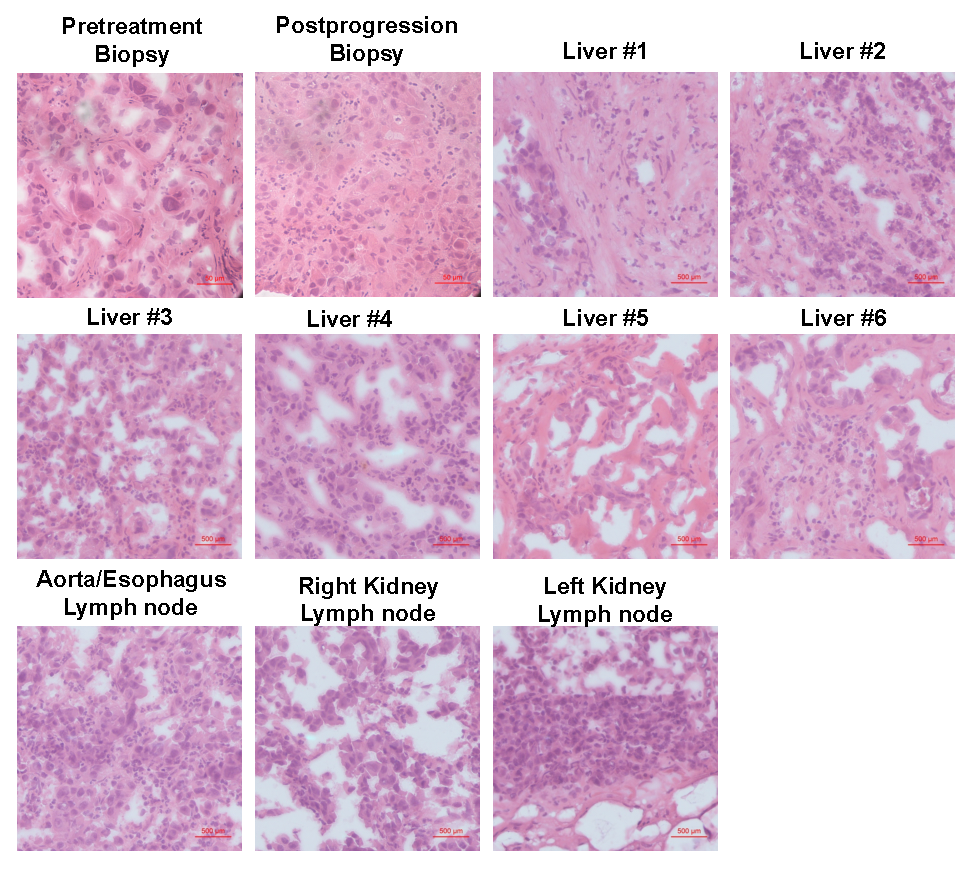
\includegraphics[width=\textwidth,keepaspectratio]{images/240/histo}
        \caption{}\label{fig:240:histo}
    \end{subfigure}
    \caption[Research autopsy of a cholangiocarcinoma patient with an FGFR2-CLIP1 fusion.]{Research autopsy of a cholangiocarcinoma patient with an FGFR2-CLIP1 fusion. (\subref{fig:240:autopsy_gross}) Gross image of the liver at the time of autopsy. (\subref{fig:240:histo}) Hematoxylin and eosin (H\&E) stains of representative slides taken from each tumor sample demonstrating abundant malignant cells.}
    \label{fig:240:autopsy}
\end{figure}
Upon death of this patient, a research autopsy was performed eight hours post-mortem. Gross examination revealed metastatic tumors involving the liver, omentum, and abdominal and retroperitoneal lymph nodes. Twenty-four liver tumor samples and 5 separate lymph nodes were procured at the time of autopsy. While we attempted to sample distinct liver tumors, the patient's liver was predominately cancerous with limited grossly normal liver tissue present (Figure~\ref{fig:240:autopsy_gross}). Samples used for subsequent analysis had at least 40\% tumor content as determined by a board-certified pathologist (Figure~\ref{fig:240:histo}).

% Table generated by Excel2LaTeX from sheet 'Sheet1'
\begin{table}[htbp]
    \centering
    {\small
    \begin{tabular}{cccccc}
         & \textbf{\% Tumor} & \textbf{Average} & \textbf{Number} & \textbf{Number} & \textbf{TMB} \\
        \textbf{Sample} & \textbf{Cells} & \textbf{Coverage (X)} & \textbf{of SNVs} & \textbf{of Indels} & \textbf{(Muts/Mb)} \\
        \hline
        Pretreatment & 40\%  & 181.19 & 44    & 6     & 1.3 \\
        Postprogression & 50\%  & 222.90 & 79    & 8     & 2.2 \\
        Liver \#1 & 50\%  & 252.23 & 101   & 13    & 2.9 \\
        Liver \#2 & 50\%  & 238.64 & 87    & 10    & 2.5 \\
        Liver \#3 & 40\%  & 229.92 & 99    & 10    & 2.8 \\
        Liver \#4 & 50\%  & 263.33 & 93    & 5     & 2.5 \\
        Liver \#5 & 40\%  & 230.61 & 56    & 9     & 1.7 \\
        Liver \#6 & 50\%  & 236.28 & 76    & 7     & 2.1 \\
        Aorta/esophagus LN & 50\%  & 236.78 & 88    & 6     & 2.4 \\
        Right Kidney LN & 40\%  & 227.86 & 73    & 11    & 2.2 \\
        Left Kidney LN & 60\%  & 216.78 & 89    & 9     & 2.5 \\
    \end{tabular}}
    \caption[Tumor content and WES metrics for each tumor sample sequenced.]{Summary of estimated tumor content and whole exome sequencing metrics within each sample. SNV: single nucleotide variant. TMB: tumor mutational burden. LN: lymph node.}
    \label{table:240:wes}
\end{table}
In total, a normal blood control and 11 tumor samples (1 pre-treatment tumor biopsy, 1 post-progression tumor biopsy, and 9 autopsy tumor samples) were chosen for further analysis (Table~\ref{table:240:wes}). Sanger sequencing confirmed that the FGFR2-CLIP1 fusion was present in each tumor sample (data not shown). DNA from these tumors were subjected to whole exome sequencing, yielding 231\texttimes{} average target coverage and revealed a total of 979 somatic variants across all tumors (292 unique somatic variants) \cite{samorodnitsky2015_hyb_amplicon}. 242 of these mutations were unique to the post-progression and autopsy samples (Supplemental File~S\thechapter{}.6). The tumor mutational burden (TMB) of samples ranged from 1.3~muts/Mb in the pre-treatment biopsy to 2.9~muts/Mb in liver sample \#1, consistent with previous studies indicating low TMB in cholangiocarcinoma \cite{chalmers2017,nakamura2015}. All tumor samples were determined to be microsatellite stable (MSS) through analysis of 2,539 loci by MANTIS \cite{kautto17}. Mutational signatures 16 and 19 were common across tumor samples. Signature 16 has been found in liver cancer and signature 19 has been found in pilocytic astrocytoma, however their etiologies are unknown \cite{cosmic_ms}.

\begin{figure}[htp]
	\centering
	\includegraphics[width=0.8\linewidth,keepaspectratio]{images/240/nj_tree}
	\caption[Neighbor joining tree over 11 cholangiocarcinoma tumor samples.]{Neighbor joining tree over 11 cholangiocarcinoma tumor samples. The tree was calculated over sets of somatic SNVs in each tumor sample, with normal defined as the empty set.}
	\label{fig:240:nj_tree}
\end{figure}
The somatic single nucleotide variants (SNVs) called in each tumor sample were subsequently used to build a phylogenetic tree of tumor samples via the neighbor joining (NJ) method \cite{saitou1987} (Figure~\ref{fig:240:nj_tree}). As expected, the pre-treatment sample branched most closely to the normal cells; the two samples are separated by a relatively short genetic distance of 33.2 indicating a high degree of genetic similarity. The post-progression sample had the next closest genetic similarity to the normal, with a genetic distance of 37.6. The liver \#1 sample was the most genetically unique tumor sample with a genetic distance of 100.1 from the normal. Liver samples \#2, 3, and 4 were clustered with the aorta/esophagus lymph node and left kidney lymph node.

\begin{figure}[htbp]
	\centering
	\begin{subfigure}{0.4\textwidth}
		\includegraphics[width=\textwidth,keepaspectratio]{images/240/canopy_tree}
		\caption{}\label{fig:240:canopy_tree}
	\end{subfigure}%
	\hfill%
	\begin{subfigure}{0.55\textwidth}
		\includegraphics[width=\textwidth,keepaspectratio]{images/240/canopy_clonal_fracs}
		\caption{}\label{fig:240:canopy_clonal_fracs}
	\end{subfigure}
	\caption[Subclonal inference from Canopy.]{Subclonal inference from Canopy. Colors in (\subref{fig:240:canopy_tree}) correspond to subclones in (\subref{fig:240:canopy_clonal_fracs}). Letters identify branches of the tree. (\subref{fig:240:canopy_tree}): Phylogenetic tree assessment with Canopy revealed four major clonal populations of cells. Each subclone is characterized by a group of mutations. MYC gain was truncal to all subclones. Clone 1 (pink) contained a unique \textit{FGFR2} N549H point mutation. Vertical distance corresponds to increased number of somatic mutations (SNVs and indels). (\subref{fig:240:canopy_clonal_fracs}) Prevalence of four tumor subclones within tumor samples.}
	\label{fig:240:canopy_results}
\end{figure}
We next utilized Canopy \cite{canopy} to computationally identify and characterize tumor subclones using both synonymous and nonsynonymous somatic SNVs, CNVs, and indels (Figure~\ref{fig:240:canopy_results}). With this analysis, we identified 4 tumor subclones across the 11 samples, with each subclone characterized by a unique group of genomic alterations (Figure~\ref{fig:240:canopy_tree}, Supplemental Files~S\thechapter{}.5, S\thechapter{}.7--8). Clones 2 (teal) and 3 (purple) were shared among all samples (Figure~\ref{fig:240:canopy_clonal_fracs}). Clone 4 (cyan) was seen in all except one autopsy sample (liver \#1) and was not present in the pre-treatment or post-treatment samples. 89\% of the tumor cells in the pre-treatment sample were estimated to be from clone 2, versus approximately 40--60\% of the other samples. Clone 1 (pink) was primarily found in liver \#1 (20\%) and at low frequency in the post-treatment sample (7\%). This is consistent with the NJ tree, as the relatively large number of mutations unique to clone 1 accounts for the distance of liver \#1 and the post-progression samples from all other samples.

\begin{table}[htp]
    \centering
    \begin{tabular}{cc}
        \textbf{Sample} & \textbf{\% Mutant} \\
        \hline
        Negative Control & 0\% \\
        Positive Control & 95\% \\
        Pretreatment & 0\% \\
        Postprogression & 0\% \\
        Liver \#1 & 17.60\% \\
        Liver \#2 & 0.30\% \\
        Liver \#3 & 0.14\% \\
        Liver \#4 & 0\% \\
        Liver \#5 & 0\% \\
        Liver \#6 & 0\% \\
        Aorta/esophagus Lymph node & 0\% \\
        Right Kidney Lymph node & 0\% \\
        Left Kidney Lymph node & 0\%
    \end{tabular}
    \caption[ddPCR for FGFR2 N549H mutation.]{Droplet digital PCR (ddPCR) results for percentage of \textit{FGFR2} N549H mutant present in samples.}
    \label{table:240:ddpcr}
\end{table}
Of the 292 distinct mutations (SNVs and indels) identified among these samples, only seven were truncal (\textit{i.e.}\ common to all four subclones). Most notable among the truncal events (branch \textbf{\textit{a}}) was a 21.9 Mb gain in chromosome 8q (chr8:124448804--146364022), containing \textit{MYC} among other genes. Although Canopy did not identify non-truncal mutations shared by clones 3 and 4, \textit{post hoc} assignment was permitted to assign mutations to a hypothetical unique common ancestor. No such mutations were assigned, suggesting that clones 3 and 4 diverged relatively early in the tumor's evolution. Of clinical interest, whole exome sequencing revealed an FGFR2 kinase domain mutation, \textit{FGFR2} N549H in a single liver tumor, liver \#1 (Figure~\ref{fig:240:nj_tree}). The \textit{FGFR2} N549H mutation occurs in the kinase hinge and has been shown to disengage the molecular breaker resulting in ligand-independent constitutive activation of the FGFR2 kinase \cite{chen2007}. The \textit{FGFR2} N549H mutation was assigned uniquely to clone 1, which was the most genetically distinct subclone compared to the patient's normal blood DNA (Figure~\ref{fig:240:canopy_tree}). Although clone 1 was predicted to be present at low frequency in the post-progression sample, \textit{FGFR2} N549H was not detected in this sample. ddPCR of all samples confirmed that the \textit{FGFR2} N549H mutation was unique to liver \#1 (Table~\ref{table:240:ddpcr}). Of the 111 mutations unique to clone 1, this mutation was estimated to be the 63\textsuperscript{rd} to occur. This led us to hypothesize that the \textit{FGFR2} N549H kinase domain mutation may have been partially responsible for driving resistance to INCB054828 in this patient, occurring along an existing clonal lineage. Driver mutation prediction with CHASM \cite{carter2009} predicted only \textit{FGFR2} N549H to be a statistically likely driver (defined as FDR-corrected $P \le 0.05$ (Supplemental File~S\thechapter{}.9).

\subsection[In vitro characterization of acquired mutations in FGFR2-CLIP1 and resistance to INCB054828]{\textit{In vitro} characterization of acquired mutations in \textit{FGFR2-CLIP1} and resistance to INCB054828}
\begin{figure}[htbp]
    \begin{minipage}[t]{0.22\textwidth}
        \vspace{0pt}
        \begin{subfigure}{\textwidth}
            \includegraphics[width=\textwidth,keepaspectratio]{images/240/fusion_rtpcr}
            \caption{}\label{fig:240:fusion_rtpcr}
        \end{subfigure}\par\vspace{0.5cm}
        \begin{subfigure}{\textwidth}
            \includegraphics[width=\textwidth,keepaspectratio]{images/240/fusion_downstream_western}
            \caption{}\label{fig:240:fusion_downstream_western}
        \end{subfigure}
    \end{minipage}
    \hfill
    \begin{minipage}[t]{0.73\textwidth}
        \vspace{0pt}
        \begin{subfigure}{\textwidth}
            \includegraphics[width=\textwidth,keepaspectratio]{images/240/fusion_ic50_curves}
            \caption{}\label{fig:240:fusion_ic50_curves}
        \end{subfigure}
    \end{minipage}
    \caption[N549H confers FGFR inhibitor resistance to the FGFR2-CLIP1 fusion.]{The FGFR2-CLIP1 fusion is sensitive to FGFR inhibitors whereas the N549H kinase domain mutation confers resistance. (\subref{fig:240:fusion_rtpcr}) RT-PCR confirmed the presence of the FGFR-CLIP1 fusion in the NIH3T3 \textit{FGFR2-CLIP1} (FC) cells and NIH3T3 \textit{FGFR2-CLIP1} N549H (N549H) cells. The fusion was not detected in the control vector (Empty) transduced cells. (\subref{fig:240:fusion_downstream_western}) Total cell lysates from NIH3T3 Empty, FC, and N549H cells were prepared and subjected to Western analysis with antibodies against: pAKT, AKT, pMEK, MEK, pMAPK, MAPK, pFGFR, FGFR, pPLCy, PLC, pFRS2, FRS2, pPI3K, PI3K, and $\beta$-actin. (\subref{fig:240:fusion_ic50_curves}) IC\textsubscript{50} curves of NIH3T3 Empty, FC, and N549H cells treated with FGFR inhibitors. Data from four replicate experiments is shown. Inhibitors include INCB054828, AZD4547, BGJ398 and JNJ42756493, ponatinib and dovitinib. }
    \label{fig:240:fusion_assays}
\end{figure}
To confirm our clinical findings that the FGFR2-CLIP1 fusion is exquisitely sensitive to INCB054828 and explore the hypothesis that the \textit{FGFR2} N549H mutation confers resistance to INCB054828, we generated NIH3T3 cells that express either a control (Empty) vector, \textit{FGFR2-CLIP1} fusion (FC), or \textit{FGFR2-CLIP1} fusion with the N549H secondary mutation (N549H) and confirmed expression by RT-PCR (Figure~\ref{fig:240:fusion_rtpcr}) and Sanger sequencing (data not shown). Western blot analyses of cells expressing the FGFR2-CLIP1 fusion demonstrated increases in PI3K/AKT, MAPK/MEK, and FGFR2 signaling pathways with or without N549H (Figure~\ref{fig:240:fusion_downstream_western}).

\begin{table}[htp]
    \centering
    \begin{tabular}{c:cccccc}
        \multicolumn{1}{c}{~} & \multicolumn{6}{c}{\textbf{IC\textsubscript{50} Values (nM)}} \\
        \hline
        & \rotatebox{270}{\textbf{INCB054828}} & \rotatebox{270}{\textbf{AZD4547}} & \rotatebox{270}{\textbf{BGJ398}} & \rotatebox{270}{\textbf{JNJ-42756493~~}} & \rotatebox{270}{\textbf{Ponatinib}} & \rotatebox{270}{\textbf{Dovitinib}} \\
        \hline
        \textit{FGFR2-CLIP1} & 10.16 & 148.59 & 108.39 & 23.28 & 166.34 & 1548.82 \\
        \textit{FGFR2-CLIP1} N549H & 1527.57 & 4764.31 & 1663.41 & 1355.19 & 162.93 & 2710.19
    \end{tabular}
    \caption[Sensitivity of FGFR2-CLIP1 WT and N549H to FGFR inhibitors.]{Sensitivity of \textit{FGFR2-CLIP1} wild-type and N549H to FGFR inhibitors. IC\textsubscript{50} values are reported for each FGFR inhibitor listed in Figure~\ref{fig:240:fusion_ic50_curves}.}
    \label{table:240:fusion_ic50}
\end{table}
To evaluate the \textit{in vitro} sensitivity of cells with the \textit{FGFR2-CLIP1} fusion and cells with \textit{FGFR2-CLIP1} N549H to the FGFR inhibitor INCB054828, we treated NIH3T3 Empty, \textit{FGFR2-CLIP1}, and \textit{FGFR2-CLIP1} N549H cells with increasing doses of INCB054828 or vehicle control (DMSO) ranging from 1.0 nM~to 5000~nM and assessed cell viability after 72 hours (Figure~\ref{fig:240:fusion_ic50_curves}). Treatment of NIH3T3 \textit{FGFR2-CLIP1} (FC) cells with INCB054828 demonstrated substantial and reproducible inhibition of cell viability with an IC\textsubscript{50} value of 10.16 nM (Table~\ref{table:240:fusion_ic50}). Consistent with our hypothesis, the \textit{FGFR2-CLIP1} N549H (N549H) cells were resistant to INCB054828 with an IC\textsubscript{50} value of 1527.57~nM\@. Empty vector control cells (Empty) were not sensitive to INCB054828, which is expected as these cells do not express endogenous FGF ligands or FGF receptors. Thus, these data help explain this patient's clinical course with his initial \textit{FGFR2-CLIP1} fusion expressing tumor responding to INCB054828 followed by acquisition of resistance via the N549H mutation.

We subsequently extended these \textit{in vitro} studies to include additional FGFR inhibitors that are currently being evaluated clinically in patients with metastatic cancer and have shown early responses in patients with FGFR-mutant cancers (Figure~\ref{fig:240:fusion_ic50_curves}). AZD4547, BGJ398, and JNJ-42756493 are selective FGFR inhibitors, whereas ponatinib and dovitinib are nonspecific tyrosine kinase inhibitors that target BCR-ABL, VEGFR, PDGFR, SRC, RET, KIT, and FLT1 in addition to FGFR\@. Our results demonstrated that FGFR2-CLIP1 cells were sensitive to AZD4547, BGJ398, JNJ-42756493, and ponatinib with IC50 values of 148.59~nM, 108.39~nM, 23.28~nM, and 166.34~nM, respectively (Table~\ref{table:240:fusion_ic50}). The \textit{FGFR2-CLIP1} N549H cells were less sensitive to BGJ398, and AZD4547, JNJ-42756493, as demonstrated by higher IC50 values than the fusion alone. Interestingly, \textit{FGFR2-CLIP1} N549H cells demonstrated similar sensitivity to ponatinib as cells with the fusion alone. Dovitinib was largely ineffective against FGFR2-CLIP1 without or with the secondary mutation. Empty vector control cells (Empty) were not sensitive to AZD-4547, BGJ398, or JNJ-42756493. However, at the highest dose (5~\textmu{}M) of ponatinib and dovitinib, the control cells (Empty) demonstrated decreased cell viability, which was not surprising as ponatinib and dovitinib are non-specific inhibitors of FGFR\@. Taken together, these data demonstrate that the FGFR2-CLIP1 fusion confers sensitivity to some, but not all, FGFR inhibitors. The \textit{FGFR2} N549H secondary mutation confers resistance to most FGFR inhibitors, but ponatinib could be used to overcome this acquired drug resistance.

\section{Discussion}
Tumor heterogeneity has been shown to have a critical role in response to therapy, development of resistance, and clinical outcome in patients with cancer \cite{choi2017,joung2017,rottenberg2012}. Rapid research autopsy has emerged as a powerful strategy to study tumor heterogeneity, as it enables essentially unlimited sampling of all sites of metastatic disease throughout the body which would otherwise not be feasible through surgical resections or tumor biopsies \cite{krook2019_review}. A number of recent studies have utilized rapid research autopsy to characterize tumor heterogeneity, clonal evolution, and mechanisms of acquired therapeutic resistance in breast, urothelial, pancreatic, and colorectal cancer. For instance, Saito \textit{et al} utilized research autopsy in breast cancer to assess trastuzumab resistance in primary versus metastatic sites \cite{saito2015}. Faltas \textit{et al} performed rapid autopsy of two patients to construct phylogenetic trees of urothelial carcinoma \cite{faltas2016}. Here, we present our findings from rapid research autopsy of a patient with metastatic cholangiocarcinoma. This is the first study to evaluate clonal heterogeneity based on exome sequencing in cholangiocarcinoma, as well as the first description of acquired resistance to INCB54828, an oral FGFR inhibitor.

Most previous and current autopsy studies utilize methods such as clonal ordering \cite{merlo2006} and neighbor joining (NJ) \cite{saitou1987} to identify and quantify relationships between different tumor regions and/or sites of metastatic cancer. In this study, we utilized the NJ method to generate a tumor-centric tree to assess similarities and differences among the pre-treatment biopsy, post-progression biopsy and nine unique tumors collected at the time of autopsy. The NJ analysis showed that the liver \#1 sample with its unique \textit{FGFR2} N549H point mutation is an outlier versus the other liver samples from autopsy. NJ and related phylogenetic methods are powerful tools to assess high-level relatedness among tumors and identify exceptional tumors, however they cannot capture the clonal heterogeneity present within discrete tumor masses or cross-seeding between sites.

Analysis of clonal evolution continues to develop as technical and computational challenges and the limited availability of large-scale autopsy data are overcome. In addition to neighbor joining, we performed subclonal inference using Canopy \cite{canopy}, which revealed 4 genetically distinct tumor subclones. Of these subclones, three were dominant across all 11 samples, with each subclone characterized by a specific set of mutations (Figure~\ref{fig:240:canopy_results}). The \textit{FGFR2} N549H mutation in clone 1 was unique to a single liver sample despite our in vitro data confirming its role as a resistance mutation. This pattern of site-unique \textit{FGFR2} resistance mutations was previously observed by Goyal \textit{et al} \cite{goyal2017} in which only 4 of 12 distinct metastatic autopsy samples were found to have acquired secondary mutations in \textit{FGFR2} serving to bypass the FGFR inhibitor effect. Each of these samples harbored unique \textit{FGFR2} mutations (K641R and N549H) with only one sample having two \textit{FGFR2} mutations (E565A and K641R)\@.  Meanwhile, the remaining 8 sites were wild-type for \textit{FGFR2}. The observations seen by Goyal \textit{et al} along with our work presented here, suggest that multiple independent drug resistance mechanisms, including FGFR-independent mechanisms, are likely contributing to tumor progression. Interestingly, in our model, clone 4 was specific to tumor samples collected at the time of autopsy, suggesting that either the biopsies missed a population of cells or that this subclone developed after the post-treatment biopsy. FOLFOX was administered after the collection of the post-treatment biopsy, but as this patient only received one dose of FOLFOX before passing away soon afterwards, we do not believe that this single dose substantially affected the heterogeneity present at time of autopsy. These findings provide evidence for the presumed notion that tumor biopsies do not accurately reflect the full complexity and heterogeneous nature of the disease. Clones 2 through 4 were seen in all autopsy samples at similar proportions. As the liver tumors were largely confluent at time of autopsy (Figure~\ref{fig:240:autopsy_gross}), multiple samples may have come from the same tumor. Another possibility is metastatic cross-seeding, as was observed by Savas \textit{et al} \cite{savas2016} using their tool superFREQ \cite{flensburg2020} for subclonal analysis of four metastatic breast cancer cases, and by Brady \textit{et al} \cite{brady2019} in pediatric osteosarcoma. Co-metastasis of multiple subclonal populations can also explain this distribution, as has been demonstrated to occur in breast ductal carcinoma \cite{casasent2018}. Clone 2 was substantially reduced in the post-treatment and autopsy samples vs.\ the pre-treatment biopsy. One potential explanation is that clone 2 was more sensitive to INCB054828 than clones 1, 3 and 4. In clone 1, the decreased sensitivity is likely due to the \textit{FGFR2} N549H point mutation, evolving from a common lineage as clone 2. Although resistance mechanisms for clones 3 and 4 could not be determined through whole exome sequencing, and driver prediction did not indicate any other likely driver mutations, we hypothesize that there can be multiple independent drug resistance adaptations within a single patient. Previous studies have demonstrated that in addition to secondary kinase domain mutations, activation in the Akt, MAPK, and PTEN pathways can mediate resistance to FGFR inhibition \cite{datta2017,goyal2017,malchers2017}. While there was no evidence for \textit{PTEN} mutations in this patient, transcriptome sequencing would be needed to assess activation of other pathways. Studies are ongoing in our laboratory to identify FGFR-independent mechanisms of resistance and to define their contributions clinically, including by RNA sequencing.

Whole exome sequencing of this patient and derivation of a phylogenetic tree suggests that ancestral genotypes can persist throughout the disease course, despite the evolution of highly derived subclones. We note that only four SNVs, three indels, and one copy number gain were detected in the trunk of this patient's phylogenetic tree (branch \textbf{\textit{a}}), indicating that development of \textit{FGFR2} fusion-positive cholangiocarcinoma may only require a small number of other initiating events (Figure~\ref{fig:240:canopy_tree}). For instance, clone 4 was only detected in autopsy samples, yet evolved from a distant ancestor to clones 1, 2 and 3. Clone 1 did not directly evolve from clone 2, but rather it shares a common ancestor with clone 2 which must have been extant before treatment (for clone 2 to be found in the pre-treatment sample). Such persistent ancestral cells may serve as an ``uncommitted'' tumor reserve capable of developing new adaptations throughout the disease course. Subclonal analysis, such as in this study, permits characterization of cancer as a dynamic process of multiple evolving and diverging cellular populations rather than a singular entity in a patient. This view of cancer permits somatic variants, a staple of cancer genomics, to be viewed in a new context. However, phylogeny inference from short-read bulk sequencing has several inherent limitations, most notably that phylogenetic solutions consistent with variant fractions and CNVs are frequently non-unique \cite{pradhan2018}. Emerging long-read and single-cell sequencing technologies will permit more certain and accurate modeling of phylogeny by directly assessing the phasing of subclonal mutations.

Lessons learned from studying molecular mechanisms of resistance to ABL, EGFR, ALK, KIT, and RAF inhibitors in human cancers have highlighted the need for next generation kinase inhibitors that are effective against acquired secondary resistance mutations \cite{demetri2011,gainor2013,hrustanovic2015,lito2013,roychowdhury2011_cml,vanallen2014}. For example, Friboulet \textit{et al} demonstrated that crizotinib induced resistance mutations in ALK-fusion positive non-small cell lung cancer (NSCLC) can be overcome by treatment with ceritinib \cite{friboulet2014}. Furthermore, mutant-selective allosteric inhibitors have shown promise in overcoming the secondary \textit{EGFR} resistance mutation T790M in NSCLC following EGFR-directed therapy \cite{jia2016}. Thus, these studies may inform strategies to overcome secondary resistance mutations to FGFR targeted therapies as several preclinical studies have demonstrated the emergence of a mutation at the gatekeeper residue or other residues within the ATP-binding pocket as well as other mutations in \textit{FGFR1--3} \cite{chell2013}. Unfortunately, several potent and selective ATP-competitive small molecule FGFR inhibitors currently in clinical trials, including INCB054828, BGJ398, AZD4547, and LY2874455, share structural similarities and are ineffective in overcoming the gatekeeper mutations \cite{chae2017}. While not considered a gatekeeper mutation, the \textit{FGFR2} N549H mutation is in the vicinity of the ATP binding pocket. Notably, our in vitro findings provide further support for the cross-resistance of multiple FGFR inhibitors, as cells harboring the secondary \textit{FGFR2} mutation N549H were resistant to INCB054828, AZD4547, BGJ398, JNJ-42756493, and dovitinib. Because of this, there has been interest in the use of structure-based drug design to develop a class of next-generation inhibitors that would overcome resistance mutations located in the FGFR2 ATP-binding pocket \cite{tan2014}. Interestingly, we demonstrated that \textit{FGFR2} N549H retained sensitivity to ponatinib. The clinical use of ponatinib in this context is supported by pharmacokinetic data in patients demonstrating a steady state ponatinib plasma concentration of 145 nM attained 4--8 hr after receiving the maximum approved dose of 45 mg \cite{cortes2012}. Unfortunately, there are serious adverse cardiovascular events associated with ponatinib, which are often dose-limiting \cite{nicolini2013}. Thus, the development of next-generation FGFR inhibitors has the potential to dramatically impact the clinical care of patients receiving FGFR targeted therapies.

In summary, this work suggests that clonal heterogeneity contributes to acquired clinical resistance to the novel FGFR inhibitor, INCB054828, in cholangiocarcinoma. Though limited to a single patient, this is the first study, to our knowledge, to define a mechanism of acquired resistance to INCB054282 through a secondary mutation to the FGFR inhibitor, INCB054828. Through rapid research autopsy and whole exome sequencing, we determine the presence of four tumor subclones and elucidate their evolution in metastatic tissues over time in a patient with FGFR2-fusion positive cholangiocarcinoma. Furthermore, we identified a post-treatment secondary kinase mutation in \textit{FGFR2}, present in a single metastatic tumor sample demonstrating the significance of intertumor heterogeneity within the same patient. We characterized the impact of the N549H mutation on sensitivity to different FGFR inhibitors \textit{in vitro}. The results of our \textit{in vitro} drug sensitivity studies suggest that this mutation conferred resistance to INCB054828 in this patient and thus may have potential as a clinically useful biomarker of resistance. Overall, our findings suggest that secondary FGFR mutations are drivers of acquired clinical resistance. Understanding these mechanisms of resistance along with FGFR kinase domain-independent mechanisms of resistance will facilitate approaches to prevent or overcome treatment resistance and disease recurrence and guide clinical strategies for these patients.

\section{List of Supplemental Files}
All supplemental files are available at \url{https://github.com/rbonneville/PhD-Dissertation/}.
\begin{enumerate}
    \renewcommand*{\labelenumi}{S\thechapter{}.\arabic{enumi}. }
    \item Annotated somatic mutations identified in each tumor sample. SNVs and indels were called with VarScan2 (Section~\ref{ssec:240:alignment_variant_calling}). Annotation was performed using ANNOVAR.
    \item Mutational signatures per tumor sample. Mutational signatures within the COSMIC Mutational Signatures set were called using deconstructSigs.
    \item Raw allele-specific CNA calls in each tumor sample. Copy number variations were called using FALCON.
    \item Manually curated CNA calls per tumor sample. Major CN corresponds to $\mathbf{W}_M$ in Canopy, minor CN to $\mathbf{W}_m$, major SD to $\mathbf{\varepsilon}_M$, and minor SD to $\mathbf{\varepsilon}_m$.
    \item Estimated subclonal composition of each tumor sample. Normal represents the estimated proportion of non-tumor cells in each sample.
    \item SNVs and indels were called with VarScan2 (Section~\ref{ssec:240:alignment_variant_calling}). Annotation was performed using ANNOVAR. ``post-progression + autopsy uniq'' contains mutations unique to the post-progression and autopsy samples (\textit{i.e.}\ absent in the pre-treatment sample), and ``autopsy unique'' contains mutations found in at least one autopsy sample but not the pre-treatment or post-progression biopsies.
    \item Each branch (\textbf{\textit{a--f}}) corresponds to a branch in Figure~\ref{fig:240:canopy_tree}. Columns C--M contain the variant fraction of each mutation in each sample, and column N contains the estimated ability score of each mutation. Higher ability scores correspond to predicted earlier development of the mutation (Section~\ref{ssec:240:subclonal_inference}).
    \item Each branch (\textbf{\textit{a--f}}) corresponds to a branch in Figure~\ref{fig:240:canopy_tree}. Note that region \texttt{chr8\_c} (chr8:124448804--146364022) had two separate copy number variations, one in branch \textbf{\textit{a}} and the other in branch \textbf{\textit{c}}.
    \item Driver mutation prediction with CHASM\@. Predicted driver mutations are indicated with CHASM FDR $\le 0.05$.
\end{enumerate}

\section*{Acknowledgements}
We would like to thank Jenny Badillo for her administrative support. We would also like to thank current and past members of the Roychowdhury Precision Cancer Medicine Team, The Ohio State Comprehensive Cancer Center, James Cancer Hospital, and community support from Pelotonia. We would most importantly like to thank this patient and his family. We would also like to thank the Ohio Supercomputer Center for computing resources.

Data used for the analyses presented in this study have been submitted to dbGaP (\url{https://ncbi.nlm.nih.gov/gap}) under the project accession number phs001830.v1.p1. The \textit{FGFR2-CLIP1} fusion gene variant and the secondary \textit{FGFR2} mutation identified in the patient have been deposited to ClinVar (\url{https://ncbi.nlm.nih.gov/clinvar/}) under the accession numbers SCV000927106 and SCV000914229.1, respectively.

\chapter[Next-generation sequencing describes clonal evolution in interdigitating dendritic cell sarcoma]{Next-generation sequencing describes clonal evolution in interdigitating dendritic cell sarcoma\footnote{This chapter previously published as: Chen HZ\cofirst, Bonneville R\cofirst, \textit{et al}. Genomic characterization of metastatic ultra-hypermutated interdigitating dendritic cell sarcoma through rapid research autopsy. \textit{Oncotarget} 2019, 10(3):277--88.}}
\label{ch:303}

\section{Introduction}
Interdigitating dendritic cell sarcoma (IDCS) is an extremely rare malignancy of dendritic cell origin with approximately 100 cases reported to date \cite{pokuri2015,xue2018}. Due to its rarity and challenging diagnosis, genomic characterization of this neoplasm has not been previously reported. Furthermore, no standard therapy exists for IDCS, which tends to affect middle-age adults with median age of diagnosis of 56.5 years \cite{saygin2013}. Localized IDCS constitutes 47\% of cases and manifests as painless lymphadenopathy, most commonly involving the cervical and axillary nodes. Isolated extra-nodal disease occurs in 25\% of cases, involving the liver, lung, spleen, bone marrow and gastrointestinal tract. Distant metastases occur in 39\% of cases and most frequently involved lymph nodes, lung, liver and bone marrow.

Here we performed whole exome sequencing (WES) of multiple tumors obtained through rapid research autopsy of a patient with metastatic IDCS. To our knowledge, this is the first time IDCS has been extensively sequenced and analyzed. Our findings demonstrate a rare ultra-hypermutated genotype, with \textgreater{}~100 somatic mutations per megabase of genome (muts/Mb) \cite{campbell2017}, characterized by distinct mutational signature profiles and clonal diversity that occurred early in the evolution of this patient's cancer. Phylogenetic analysis revealed inactivation of \textit{TP53} and \textit{CDKN2A} (\textit{p16\textsuperscript{INK4a}/p19\textsuperscript{ARF}}) as well as amplification of \textit{c-KIT} and \textit{PDGFR}$\mathit{\alpha}$ as truncal alterations. We further detected amplification of \textit{APOBEC3A--H} encoding cytidine deaminases on chromosome 22q that may have contributed to the ultra-hypermutation. In summary, our work describes the genomic landscape and clonal heterogeneity of an ultra-rare cancer through the innovative approach of research autopsy. 

\section{Materials and Methods}
\subsection{Research autopsy}
The patient was consented to an Institutional Review Board (IRB)-approved clinical study for tumor profiling and body donation (Figure~\ref{fig:240:autopsy_flowchart}). At time of death, the patient's next-of-kin (and/or hospice agency) notified members of the research team. The deceased was transported to the OSU Medical Center and a limited research autopsy was conducted within 3 hours after patient's passing. Metastatic tumors and adjacent normal tissues were sampled and immediately archived as fresh frozen specimens in OCT medium. After conclusion of the autopsy, the deceased was transported back to the designated funeral home within 24 hours. 

\subsection{Whole exome sequencing}
We extracted genomic DNA from frozen tumors and normal (blood) samples and prepared sequencing libraries using an established protocol \cite{samorodnitsky2015_hyb_amplicon} that included enrichment with the xGen Exome Research Panel v1.0 from Integrated DNA Technologies. Sequencing was performed on an Illumina HiSeq 4000 at The Genomics Services Laboratory at Nationwide Children's Hospital (Columbus, Ohio) and achieved a median depth of 100--286\texttimes{}. 

\subsection{Alignment, variant calling, and annotation}
\label{ssec:303:align_vars_anno}
Sequencing reads were aligned to hg19 using BWA \cite{bwa} version 0.7.14, deduplication using Picard \cite{Picard2019toolkit} version 2.3.0, and quality recalibration and local realignment around indels performed with Picard and GATK \cite{mckenna10} version 3.5 as previously described (Section~\ref{ssec:240:alignment_variant_calling}). Somatic SNVs (single nucleotide variations), somatic indels, and germline SNVs were called using VarScan2 \cite{varscan2} version 2.3.9, filtered using bam-readcount \cite{bamreadcount}, and annotated with ANNOVAR \cite{annovar} (revision \#11f4bb, 2016-02-01) (Section~\ref{ssec:240:alignment_variant_calling}). Mutational signatures from the COSMIC Mutational Signatures set \cite{cosmic_ms} were called with deconstructSigs \cite{rosenthal16} version 1.8.0 with default settings and exome2genome trinucleotide frequency correction, run on R version 3.3.2. Microsatellite instability testing was performed using MANTIS \cite{kautto17} version 1.0.3, run with three threads and otherwise default settings (Section~\ref{ssec:msilandscape:tool_params}). Neighbor-joining trees were computed over the sets of somatic SNVs from all tumor samples as previously described (Section~\ref{ssec:240:nj_methods}). Allele-specific copy number variants (CNVs) were called using FALCON \cite{falcon} followed by manual curation (Section~\ref{ssec:240:cnv_methods}).

\subsection{Subclonal phylogenetic analysis}
\label{ssec:303:phylo_analysis}
The reference read count, alternate allele count, and variant fractions of all nonsynonymous somatic variants called within each tumor sample were compiled as previously described (Section~\ref{ssec:240:canopy_mut_filtering}). As this yielded 893 mutations in this patient, we downsampled to a set of 60 mutations with maximal diversity using a high correlation filter, implemented as follows:
\begin{algorithm}[H]
    \caption{Mutation set downsampling}
    \label{alg:303:mutation_downsampling}
    \begin{algorithmic}[1]
        \While{$|M| > n$}
            \State $i \gets \argmax_x (\rho_{M_x M_y}) \qquad y > x; \quad x,y \in 1 \twodots |M|$
            \State $M \gets M \setminus \{M_i\}$
        \EndWhile
    \end{algorithmic}
\end{algorithm}
\noindent where $M$ is the set of mutations, with each mutation being a vector of its per-sample VFs, $n$ is the desired final number of mutations (in this case, $n = 60$), and $\rho$ is the correlation between VFs in each sample, defined as follows:
\begin{equation}
    \rho_{\vec{a} \vec{b}} = \frac{\cov(\vec{a} \vec{b})}{\sigma_{\vec{a}} \sigma_{\vec{b}}}
\end{equation}
where $\cov(\vec{x}, \vec{y})$ is the covariance between elements of same-length vectors $\vec{x}$ and $\vec{y}$, and $\sigma_{\vec{x}}$ is the population standard deviation of elements of vector $\vec{x}$. Canopy was then run as previously described (Section~\ref{ssec:240:canopy_tree}) followed by \textit{post hoc} assignment of SNVs not used for tree-building (including SNVs removed by downsampling) and indels (Section~\ref{ssec:240:tree_assignment}).

\section{Results}
\subsection{Clinical course}
\begin{figure}[htp]
    \begin{center}
        \includegraphics[width=\textwidth,keepaspectratio]{images/303/clinical_course}
    \end{center}
    \vspace{-0.3cm}
    \caption[Clinical course of a patient with metastatic IDCS.]{Clinical course of a patient with metastatic IDCS. Summary of treatment history and tumor response/progression of the patient. Research autopsy was performed 3 hours post-mortem. SRS: stereotactic radiosurgery.}
    \label{fig:303:clinical_course}
\end{figure}
Our patient was a 57-year old Caucasian male who developed an isolated FDG-avid 2.4~\texttimes{}~2.4~cm right-sided neck mass on PET scan in 2016. Biopsy result of this mass showed a ``pleomorphic\slash{}spindle cell neoplasm.'' Immunohistochemical (IHC) analyses demonstrated focal CK7 staining. Clinical evaluation revealed no primary lesion involving the skin or oropharynx. In August 2016, he underwent modified radical right neck dissection and partial submandibular gland excision with one level I lymph node demonstrating complete tumor involvement and suspicious for extranodal extension; remaining lymph nodes (0/29) from levels II, III and IV were negative for tumor infiltration. IHC on the surgical specimen showed positivity for S100, SOX10 and CK7. A diagnosis of IDCS was issued. Given his localized presentation, he received adjuvant radiation to the right level IB--III nodes with a boost to the primary site of disease. In November 2016, he initiated adjuvant nivolumab (3~mg/kg every 2~weeks) given FoundationOne\textsuperscript\textregistered{} report showing \textgreater{}~100~muts/Mb in his tumor. Following adjuvant immunotherapy, he developed metastatic recurrence that failed to respond to subsequent treatments including combination immunotherapy (CTLA-4/PD-1 inhibitors), chemotherapy and molecularly targeted therapies.  His clinical course leading up to the research autopsy is summarized in Figure~\ref{fig:303:clinical_course}.

\begin{figure}[htbp]
	\centering
	\begin{subfigure}{0.72\textwidth}
		\includegraphics[width=\textwidth,keepaspectratio]{images/303/ct}
		\caption{}\label{fig:303:ct}
	\end{subfigure}%
	\hfill%
	\begin{subfigure}{0.235\textwidth}
		\includegraphics[width=\textwidth,keepaspectratio]{images/303/histo}
		\caption{}\label{fig:303:histo}
	\end{subfigure}
	\caption[Research autopsy of a patient with metastatic IDCS.]{Research autopsy of a patient with metastatic IDCS. (\subref{fig:303:ct}) CT scans depicting organs with metastatic cancer; brain (panel 1, yellow), hilar lymph node (2), liver (3--4), rib (5) and pelvis (6). Arrowheads and dashed circles indicate tumors; asterisks indicate tumors procured at research autopsy. (\subref{fig:303:histo}) H\&E stained frozen sections of metastatic tumors in brain, lung, liver and rib procured from research autopsy. Sections demonstrate high tumor cell content. Enlarged inset at bottom right of each image panel shows dysplastic nuclei with mitotic figures.}
	\label{fig:303:tumor_images}
\end{figure}
Prior to his death, the patient was consented to an IRB-approved research autopsy study for patients with advanced cancers. CT scans obtained prior to hospice enrollment showed tumor involvement of multiple organs (Figure~\ref{fig:303:ct}) and were used to guide sample procurement at time of research autopsy, which was performed within three hours post-mortem. A total of twenty-four metastatic tumor samples were procured from involved organ sites. A pathologist assessed the viability and tumor cell content of autopsy samples (Figure~\ref{fig:303:histo}) prior to selection for genomic studies.

\subsection{Genomic characterization of IDCS}
\begin{table}[ht]
    \centering
    {\footnotesize
    \setlength{\tabcolsep}{2.9pt}
    \begin{tabular}{ccccccccc}
        & \textbf{Organ} & \textbf{\% Tumor} & \textbf{Median} & & \textbf{TMB} & \textbf{\#} & \textbf{\#} & \\
        \textbf{Sample} & \textbf{Involved} & \textbf{Cells} & \textbf{Coverage} & \textbf{\% 100\texttimes{}} & \textbf{(muts/Mb)} & \textbf{SNVs} & \textbf{Indels} & \textbf{MANTIS} \\
        \hline
        T1  & Biopsy (Bx) & 30\%  & 100   & 50.10  & 131.5 & 5,091 & 21    & 0.326 \\
        T2  & Left lung (L.lung) & 80\%  & 213   & 79.83 & 158.4 & 6,139 & 22    & 0.330 \\
        T3  & Right lung (R.lung) & 90\%  & 245   & 84.19 & 165.3 & 6,408 & 19    & 0.330 \\
        T4  & Liver1 & 90\%  & 218   & 82.12 & 163.3 & 6,329 & 20    & 0.328 \\
        T5  & Liver2 & 80\%  & 233   & 83.38 & 158.8 & 6,160 & 15    & 0.327 \\
        T6  & Liver3a & 80\%  & 270   & 87.01 & 150.4 & 5,826 & 22    & 0.318 \\
        T7  & Liver3b & 90\%  & 286   & 87.88 & 156.1 & 6,050 & 19    & 0.324 \\
        T8  & Rib   & 80\%  & 272   & 86.70  & 148.9 & 5,776 & 15    & 0.319 \\
        T9  & Right iliac (R.iliac) & 90\%  & 242   & 85.20  & 167.0   & 6,473 & 20    & 0.330 \\
        T10 & Brain & 50\%  & 257   & 86.80  & 130.1 & 5,043 & 15    & 0.320 \\
    \end{tabular}}
    \caption[Sample characteristics and sequencing metrics.]{Sample characteristics and sequencing metrics. A board-certified pathologist estimated the percentage of tumor cells in each sample. Liver3a and Liver3b samples were procured from two different regions of a large liver tumor. The pre-treatment biopsy sample was obtained from a formalin-fixed paraffin-embedded surgical specimen, while autopsy tumor samples were frozen in OCT\@. \% 100\texttimes{} indicates the percent of variants in each tumor sample with at least 100\texttimes{} coverage. TMB includes synonymous and nonsynonymous SNVs as well as insertions/deletions (indels). \#~SNVs and \#~Indels columns indicate the total number of somatic SNVs and indels detected in each tumor sample. Microsatellite status was determined using MANTIS, with scores \textless{}~0.4 indicating microsatellite stability (MSS).}
    \label{table:303:wes_samples}
\end{table}
We performed WES on nine metastatic tumors and the resected pre-treatment tumor (Table~\ref{table:303:wes_samples}). Calculation of tumor mutational burden (TMB), including single nucleotide variants (SNVs) and insertions/deletions (indels), demonstrated ultra-hypermutation (130.1--167.0~muts/Mb) in all tumors analyzed (Supplemental File~S\thechapter{}.1). Interrogation of microsatellite status utilizing MANTIS \cite{kautto17} showed that all tumors were microsatellite stable (MSS) despite their ultra-hypermutation. 

To further characterize this patient's cancer, we investigated whether specific substitution mutational signatures, which arise due to different mutagenic processes \cite{alexandrov2013}, may be present. This analysis revealed the presence of signature 2 (APOBEC), signature 7 (UV light) and signature 11 (alkylating agent), which are all characterized by C\textgreater{}T substitutions, in all tumor samples (Figure~\ref{fig:303:mutational_spectra_by_sample}, Supplemental File~S\thechapter{}.2). Of the three mutational signatures, signature 7 had the highest prevalence.

\begin{figure}[htbp]
	\centering
	\begin{subfigure}{0.23\textwidth}
		\includegraphics[width=\textwidth,keepaspectratio]{images/303/variants_by_category}
		\caption{}\label{fig:303:variants_by_category}
	\end{subfigure}%
	\hfill%
	\begin{subfigure}{0.72\textwidth}
		\includegraphics[width=\textwidth,keepaspectratio]{images/303/mutation_heatmap}
		\caption{}\label{fig:303:mutation_heatmap}
	\end{subfigure}\par\vspace{0.3cm}
	\begin{subfigure}{0.9\textwidth}
	    \includegraphics[width=\textwidth,keepaspectratio]{images/303/nj_tree}
	    \caption{}\label{fig:303:nj_tree}
	\end{subfigure}
	\caption[Classification of somatic variants and NJ tree.]{Classification of somatic variants and construction of neighbor joining (NJ) tree. (\subref{fig:303:variants_by_category}) The 7,417 somatic variants detected in all ten tumor samples T1--10 from this patient were classified into three categories: Ubiquitous (Ubi.), present in all ten tumor samples; Shared (Sha.), present in some but not all ten tumor samples; Private (Priv.), present in only one tumor sample. Percentage of each variant category are as indicated in the bar graph. Somatic variants analyzed include single nucleotide variants (SNVs) and insertions/deletions (indels). (\subref{fig:303:mutation_heatmap}) Heatmap demonstrating distribution and variant allele frequency (VAF) of the 7,417 somatic variants in ten tumor samples T1--10. Color intensity corresponds to VAF\@. (\subref{fig:303:nj_tree}) NJ tree depicting the evolutionary relationship of the ten tumor samples T1--10 from this patient. Normal represents hypothetical population of wild-type cells without somatic aberrations. The 3,642 ubiquitous variants included driver mutations in \textit{TP53} and \textit{CDKN2A} as well as the \textit{RPA2} variant predicted to have loss-of-function. Branch lengths correspond to the genetic distance between samples. T1--10 correspond to samples listed in Table~\ref{table:303:wes_samples}.}
	\label{fig:303:variants_plots}
\end{figure}
We next classified the 7,417 somatic variants (SNVs and indels) in all ten tumor samples of this patient into three categories: Ubiquitous, Shared, and Private (Figure~\ref{fig:303:variants_plots}). Ubiquitous variants are variants detected in all tumor samples and included driver mutations in \textit{TP53} and \textit{CDKN2A}, while shared variants are those detected in subsets of tumor samples. Finally, private variants are variants unique to each tumor sample. A tumor-centric evolutionary tree was constructed based on the pairwise genetic distance, as measured by number of discordant SNVs, between the wild-type cells (normal) and tumor samples in this patient (Figure~\ref{fig:303:nj_tree}). Finally, we interrogated the prevalence of copy number variations (CNVs) using the allele-specific CNV caller FALCON. After manual review and curation, 29 unique CNVs including amplification (including \textit{c-KIT}, \textit{PDGFR}$\mathit{\alpha}$, and \textit{APOBEC3A--H}), deletion and loss-of-heterozygosity events were detected (Figure~\ref{fig:303:cnv_plots} and Supplemental Files~S\thechapter{}.3--4).

\subsection{Reconstructing clonal evolution}
\label{ssec:303:clone_results}
\begin{figure}[htbp]
	\centering
	\begin{subfigure}{0.4\textwidth}
		\includegraphics[width=\textwidth,keepaspectratio]{images/303/canopy_tree}
		\caption{}\label{fig:303:canopy_tree}
	\end{subfigure}%
	\hfill%
	\begin{subfigure}{0.55\textwidth}
	    \includegraphics[width=\textwidth,keepaspectratio]{images/303/canopy_P}
	    \caption{}\label{fig:303:canopy_P}
	\end{subfigure}\par\vspace{0.1cm}
	\begin{subfigure}{0.5\textwidth}
	    \includegraphics[width=\textwidth,keepaspectratio]{images/303/sigs_per_branch}
	    \caption{}\label{fig:303:sigs_per_branch}
	\end{subfigure}
	\caption[Analysis of cancer phylogeny and clonal evolution.]{Analysis of cancer phylogeny and clonal evolution. (\subref{fig:303:canopy_tree}) Phylogram constructed using Canopy integrating SNVs, curated CNVs and indels detected through WES of tumor samples T1--10. Output from Canopy includes number of clones, clonal fractions and mutational groups (\textbf{\textit{a--j}}) associated with each clone. Given the large number of somatic SNVs in this ultra-hypermutated cancer, downsampling of SNVs was performed in addition to following recommended parameters for Canopy tree building. Somatic SNVs not utilized by Canopy as well as indels were retroactively assigned based on VAF patterns to mutational groups \textbf{\textit{a--j}} using a maximal likelihood model. Based on this analysis, six different clones of tumor cells were identified in this patient's cancer. Truncal or group a mutations are common or ancestral to all clones of tumor cells. In contrast, mutations in groups \textbf{\textit{b}}, \textbf{\textit{d}}, \textbf{\textit{f}}, \textbf{\textit{h}}, and \textbf{\textit{j}} are private to clones 1, 2, 3, 4, and 6, respectively. The length of horizontal branches in the tree is proportional to the number of mutations. (\subref{fig:303:canopy_P}) Stacked bar graph depicting the percentage of different clonal tumor cell populations as estimated by Canopy in each sample. (\subref{fig:303:sigs_per_branch}) Mutations in each branch of the phylogram estimated by Canopy were called with deconstructSigs, utilizing the COSMIC Mutational Signatures set. Signature 7 (UV) was detected in every branch of the tumor's evolutionary history. T1--10 correspond to samples listed in Table~\ref{table:303:wes_samples}.}
	\label{fig:303:canopy_results}
\end{figure}
Integrating the above genomic data (SNVs, indels and CNVs), we used the program Canopy \cite{canopy} to synthesize a hypothetical model of the clonal evolution of this patient's cancer (Figure~\ref{fig:303:canopy_tree}). Canopy identified six genetically distinct clonal populations of tumor cells, present in various proportions within each tumor (Figure~\ref{fig:303:canopy_P}, Supplemental File~5). These six clones are differentiated by ten unique groups of genomic alterations (\textbf{\textit{a--j}}, Supplemental Files~S\thechapter{}.6--7), which all contained mutational signature 7 (Figure~\ref{fig:303:sigs_per_branch} and Supplemental File~S\thechapter{}.2). Of note, group \textbf{\textit{a}} contains truncal alterations ancestral to all tumor cells including two well-documented driver mutations, \textit{TP53} P278L and \textit{CDKN2A} R80X, which were classified as ubiquitous. Interestingly, we also detected a truncal variant \textit{RPA2} V108L\@. \textit{RPA2} encodes a subunit of the heterotrimeric Replication Protein A complex that is critical for DNA replication, repair, recombination and DNA damage response \cite{byrne2019}. Finally, we identified two notable truncal amplifications of regions on the long arms of chromosome 4 (\textapprox{}17.2~Mb), containing \textit{c-KIT} and \textit{PDGFR}$\mathit{\alpha}$, and chromosome 22 (\textapprox{}24.6~Mb), containing \textit{APOBEC3A--H} (Figure~\ref{fig:303:cnv_plots}).

\section{Discussion}
Extensive multi-regional sequencing of tumors revealed the complex genetic landscape of treatment-refractory cancers by demonstrating intratumor heterogeneity \cite{gerlinger2012,gerlinger2014}, which underscores the limitations of tumor profiling with tissue derived from a single biopsy specimen. From a clinical perspective, tumor heterogeneity contributes to the incomplete therapeutic responses seen in patients receiving different types of anti-cancer therapies including molecularly targeted therapies. Mechanistically, tumor heterogeneity drives acquired therapeutic resistance by facilitating the selection and expansion of therapy-resistant clones. Research autopsy has emerged as a powerful approach to characterize tumor heterogeneity at different metastatic sites in the individual patient. Together with information from treatment-na\"ive samples, sequencing of metastatic tumor samples from autopsy can provide a comprehensive molecular portrait of advanced cancers that reflects changes in tumor cell populations and genomes over time \cite{faltas2016,juric2015}. Here we performed research autopsy on a patient with widely metastatic IDCS. Genomic profiling of his tumors revealed somatic ultra-hypermutation and tumor heterogeneity in the form clonal diversity. Recently, Campbell \textit{et al} demonstrated a prevalence of ultra-hypermutation (TMB \textgreater{}~100~muts/Mb) of 0.6\% in a cohort of 78,452 adult cancers \cite{campbell2017}. Therefore, the rare histologic classification of IDCS in this patient is accompanied by a rare `genotype' of ultra-hypermutation.

Hypermutation in cancer may arise from intrinsic defects in DNA damage repair pathways or extrinsic mechanisms such as mutagenic exposure \cite{campbell2017}. The majority of ultra-hypermutation detected by Campbell et al. was attributed to mutations in mismatch repair (MMR) genes and replication-associated DNA polymerases POL$\varepsilon$ or POL$\delta$ (Section~\ref{ssec:intro:dna_replication}--\ref{ssec:intro:mutation}). While we did not detect genomic alterations involving MMR or POL$\varepsilon$\slash{}POL$\delta$ to explain this patient's ultra-hypermutated cancer, we did detect a truncal amplification of a region on chromosome 22q containing genes encoding the APOBEC3A--H (or A3 subfamily) cytidine deaminases. The deregulated expression and activity of A3A and A3B have been linked to cancer development through enhanced DNA hypermutation and unfaithful RNA editing \cite{salter2016,burns2013,henderson2015}. Furthermore, we identified a truncal \textit{RPA2} variant with a predicted (by DUET \cite{pires2014}) destabilizing missense mutation in the C-terminal winged helix domain important for protein-protein interaction that could have further contributed to defective DNA damage repair and hypermutation. Together with driver mutations in tumor suppressors \textit{TP53} and \textit{CDKN2A}, the above events could have produced ultra-hypermutation as seen in this patient's cancer.

Different models of mutation accumulation have been proposed for hypermutated cancers and could be classified as `steady' versus `dynamic' hypermutation \cite{campbell2017}. In the steady model, mutations accumulate gradually due to continuous mutagenic exposure or germline MMR deficiencies, leading to hypermutation over time. The dynamic model, seen in cancers with POL$\varepsilon$ or POL$\delta$ mutations, is characterized by `bursts' of mutations followed by rise in genome-wide TMB. Through analyses of clonality and mutational signatures, we hypothesize a gradual mode of hypermutation consistent with the former model in our patient's cancer. Genomic profiling of treatment-na\"ive tumor revealed high TMB at baseline that may have been the result of UV exposure, producing the driver mutations in \textit{TP53} and \textit{CDKN2A}\@. TMB analysis of his autopsy tumor samples demonstrated an increase of \textapprox{}20--37 additional muts/Mb that could be attributed to the truncal amplification of the A3 subfamily of cytidine deaminases, as indicated by the presence of APOBEC-specific signature 2, and/or potentially therapy-induced mutations. Interestingly, the brain metastasis (T10) was the only autopsy tumor sample that had similar TMB as the treatment-na\"ive tumor (T1) while still retaining the APOBEC signature. A technical explanation underlying this finding may be due to lower tumor cell contents in both samples affecting variant detection. Alternatively, this may reflect similar biology between the treatment-na\"ive tumor sample obtained from neck surgery and the brain metastasis; this similarity is demonstrated by the shorter genetic distance between `normal' and T1 or T10 samples relative to other tumor samples in the NJ tree. Finally, the genetic dissimilarity between the brain metastasis and tumor samples from other organs also suggests the presence of unique genetic features of cancer cells with increased propensity for invasion of the central nervous system. Although high TMB has been established as a clinically useful biomarker of response to checkpoint blockade in multiple human cancers \cite{yarchoan2017,gibney2016}, our patient developed progressive cancer while receiving adjuvant therapy with the PD-1 inhibitor nivolumab and had disease progression while being treated with dual \mbox{CTLA-4/PD-1} blockade. Therefore, his case highlights the need for identification of additional biomarkers to predict clinical benefit for immunotherapy in patients with hypermutated cancers.

In summary, we present the first genomic characterization of metastatic IDCS, an extremely rare neoplasm of dendritic cell origin that lacks any standard therapy. This patient had metastatic IDCS characterized by ultra-hypermutation and clonal heterogeneity, likely through a combination of chronic mutagen exposure (UV), acquired defects in pathways important for DNA repair (\textit{TP53}, \textit{CDKN2A}, \textit{RPA} mutations), and gain of genes that promote DNA hypermutation (\textit{APOBEC3A--H})\@. His cancer was aggressive and refractory to multiple anti-cancer therapies including molecularly targeted agents and immunotherapies. In the future, it will be important to study additional patients with this and other rare cancers with hypermutation. Finally, the broader clinical implication of our results is that although patients with hypermutated cancer, originating from either somatic or germline genomic aberrations, are more likely to benefit from checkpoint inhibition, research is still needed to stratify these patients to maximize therapeutic efficacy and identify the different genetic determinants of primary or acquired resistance to immunotherapy.

\section{List of Supplemental Files}
All supplemental files are available at \url{https://github.com/rbonneville/PhD-Dissertation/supplemental_files}.
\begin{enumerate}
    \renewcommand*{\labelenumi}{S\thechapter{}.\arabic{enumi}. }
    \item Annotated mutations by tumor sample. SNVs and indels passing quality control filters (Section~\ref{ssec:303:align_vars_anno}) were annotated using ANNOVAR.
    \item Mutational signatures per tumor and per phylogeny branch. Mutations in each tumor and each branch were called with deconstructSigs, utilizing the COSMIC Mutational Signatures set.
    \item Allele-specific CNVs were called using FALCON with the QC procedure provided with Canopy. Output prior to manual curation is provided in this file.
    \item For each of the 29 CNV-affected regions identified and manually curated, the major and minor copy number and standard deviations are listed. These values were determined through execution of FALCON with manual selection of SNVs for segmentation.
    \item Estimated clonal composition of all tumor samples. For each of 10 tumor samples, the estimated fraction of normal and tumor cells from each clone is listed.
    \item Annotated mutations by phylogeny branch. SNVs and indels are listed for each branch \textbf{\textit{a--j}} of the phylogram (Figure~\ref{fig:303:canopy_tree}). Mutations in bold were used by Canopy to build the tree, and the remaining mutations were retroactively assigned to the tree (Section~\ref{ssec:303:phylo_analysis}).
    \item Curated CNVs by phylogeny branch. For each of the 29 CNV-affected regions identified and manually curated, the per-subclone major and minor copy number as estimated by Canopy is listed.
\end{enumerate}

\section*{Acknowledgements}
We are grateful for administrative support from Jenny Badillo, the Comprehensive Cancer Center, community support from Pelotonia, and most importantly the patient and his family. We thank the Ohio Supercomputer Center (OSC) for providing us with the computing power and resources for the analyses in this report.

\chapter[Integrated genomic and transcriptomic analysis of small cell lung cancer]{Integrated genomic and transcriptomic analysis of small cell lung cancer\footnote{This chapter currently accepted for publication as: Chen HZ\cofirst, Bonneville R\cofirst, Paruchuri A\cofirst, \textit{et al}. Genomic and transcriptomic characterization of relapsed small cell lung cancer through rapid research autopsy. \textit{JTO Clinical and Case Reports}.}}
\label{ch:sclc}

\section{Introduction}
Small cell lung cancer (SCLC) is a lethal neuroendocrine malignancy accounting for 13--15\% of new lung cancer cases annually worldwide \cite{sabari2017,siegel2019}. Most SCLC patients present with initially chemotherapy-sensitive disease, but almost all will experience progression or relapse leading to death. In 2019, combination chemotherapy and immunotherapy was FDA-approved as first-line treatment for metastatic SCLC \cite{horn2018,pazares2019}, with modest two-month improvement in survival compared to chemotherapy alone. For decades, topotecan was the only FDA-approved second-line chemotherapy with objective response rate (ORR) of 10--20\% \cite{pawel1999}, until lurbinectedin was granted accelerated approval in 2020 based on a phase II trial showing 35\% ORR \cite{trigo2020}. Despite these recent approvals, there is an urgent need to develop more effective therapies for advanced SCLC\@.

Key studies in the last decade have profiled the mutational landscape of primary SCLC, driven by \textit{TP53} and \textit{RB1} inactivation \cite{george2015,rudin2012,peifer2012}. Furthermore, distinct SCLC subgroups have been identified based on the expression of key transcription factors including ASCL1 and NEUROD1 \cite{rudin2019,baine2020}. How each SCLC subtype confers different clinical phenotypes and differential response to anti-cancer therapies is under active investigation \cite{gay2021}, with the goal of delivering precision therapy to SCLC patients by matching each SCLC subtype to specific treatments. 

Molecular characterization of relapsed SCLC has been hampered by tissue scarcity due to rapid clinical deterioration of relapsed patients. Therefore, unlike for primary SCLC, less is known about the genomic and transcriptomic landscapes of relapsed SCLC and mechanisms that mediate therapeutic resistance, although recent non-autopsy studies on relapsed SCLC have begun to address this knowledge gap. For example, Gardner \textit{et al} used patient-derived xenografts of paired chemosensitive and chemoresistant SCLC tumors to elegantly demonstrate that acquired chemoresistance occurred through epigenetic silencing of a DNA damage repair factor, \textit{SLFN11} \cite{gardner2017}. Wagner \textit{et al} performed genomic profiling on a cohort of relapsed SCLC patients and identified recurrent Wnt pathway alterations as a mechanism of acquired chemoresistance \cite{wagner2018}. Weiss \textit{et al} performed genome-wide exome and RNA-seq on twelve SCLC patients who relapsed after platinum-based chemotherapy \cite{weiss2017}. Aside from driver mutations in \textit{RB1} and \textit{TP53}, the authors identified few recurrent targetable genomic alterations in this cohort of patients. Finally, an important study by Stewart \textit{et al} performed single cell sequencing of circulating tumor cells (CTCs) and CTC-derived xenografts from platinum-sensitive and refractory SCLC patients and demonstrated an association between increased intratumoral heterogeneity and chemoresistance \cite{stewart2020}. The latter study is one of the first non-autopsy studies to directly evaluate intratumor heterogeneity in advanced SCLC\@. Overall, however, further study of relapsed SCLC is needed to identify additional targetable mechanisms underlying therapeutic resistance, including resistance to immunotherapy which is now approved for front-line treatment in the metastatic setting. 

The utilization of tumor specimens from rapid research autopsy has accelerated the study of tumor heterogeneity and acquired resistance in advanced cancer (Section~\ref{ssec:intro:heterogeneity_methods}) \cite{krook2019_review}. To our knowledge, this is the first study to perform whole exome and transcriptome profiling of advanced SCLC through research autopsy. From exome sequencing, we inferred intertumor and intratumor clonal heterogeneity arising from branched and linear evolution, while transcriptome analyses supported the subtype-specific suppression of adaptive anti-tumor immunity in primary and advanced SCLC\@. Our results provide new insights into the subclonal architecture of advanced SCLC and identify new potentially targetable pathways involved in anti-tumor immune responses.

\section{Materials and Methods}
\subsection{Rapid research autopsy}
Informed consents were obtained from five patients with advanced SCLC to participate in an IRB-approved clinical study for tumor profiling by next-generation sequencing (NGS) and body donation (NCT02090530) \cite{krook2019_review,krook2019_mcs}. Deceased patients were transported to The Ohio State University Regional Autopsy Center, where research autopsy for tumor procurement was performed no more than 16 hours after patients' passing. CT imaging when available was used to guide procurement from organs with cancer. After autopsy completion, the deceased were transported to a designated funeral home within 24 hours.

\subsection{Tumor DNA/RNA sequencing}
Samples with tumor cell content \textgreater{}60\% and without significant necrosis were selected for NGS analyses. Genomic DNA and total RNA were extracted using Qiagen kits per manufacturer's protocol. Libraries were prepared following established protocols (TruSeq Stranded Total RNA with Ribo-Zero Gold\textsuperscript\textregistered{} from Illumina) \cite{krook2019_mcs,reeser2017}, enriched with the xGEN Exome Research Panel v1.0 (IDT), and sequenced on an Illumina HiSeq 4000.

In addition, we utilized RNA-seq data of primary and relapsed SCLC and normal lung tissue obtained from previous publications \cite{rudin2012,wagner2018,weiss2017,fagerberg2014}. Of these data sets, one had paired primary SCLC and normal lung samples \cite{rudin2012}, while the rest contained either exclusively tumor \cite{wagner2018,weiss2017} or normal samples \cite{fagerberg2014}. Non-SCLC RNAseq data \cite{tcgaluad,tcgalusc} were downloaded from The Cancer Genome Atlas via the Genomic Data Commons (GDC) data portal (\url{https://portal.gdc.cancer.gov/}). We randomly chose a subset of 60 and 49 tumor-normal paired samples of lung adenocarcinoma and squamous cell carcinoma, respectively, for ssGSEA and ImSig analyses.

\subsection[ctDNA sequencing]{Circulating tumor DNA (ctDNA) sequencing}
ctDNA was isolated using QIAamp Circulating Nucleic Acid Kit per manufacturer's protocol. An input of 300~ng was used to generate libraries for paired-end sequencing on a NextSeq instrument achieving median coverage of \textapprox{}500\texttimes{} \cite{griffith2015}.

\subsection[SNVs and CNVs, clonal inference, and mutational signatures]{Somatic mutation and copy number variant calling, clonal inference, and mutational signatures}
These bioinformatics analyses were performed as previously described (Section~\ref{sec:240:methods}). Briefly, sequencing reads were aligned to hg19 using bwa \cite{bwa}, deduplication performed with Picard \cite{Picard2019toolkit}, and base quality score recombination and realignment around indels with GATK \cite{mckenna10}. Variants were called with VarScan2 \cite{varscan2} and allele-specific CNVs with FALCON \cite{falcon}. Clonal inference was performed using Canopy \cite{canopy}, and mutational signatures were inferred with deconstructSigs \cite{rosenthal16}. Bradley-Terry modeling was used to estimate relative ordering of mutations in the phylogeny branches of SCLC autopsy patients as previously described (Section~\ref{ssec:240:mutational_ordering}).

\subsection{Clonal fraction estimation in ctDNA}
\label{ssec:sclc:ctdna_clones}
\subsubsection{Definitions}
\newcommand*{\CM}{\mathbf{\tilde{C}^\text{M}}}
\newcommand*{\Cm}{\mathbf{\tilde{C}^\text{m}}}
To be solved is the probability vector $\hat{\theta}$ such that:
\begin{equation}
    \hat{\theta} = \argmax_{\vec\theta} \mathcal{L}\left(\vec{\theta} | \vec{r}, \vec{x},\vec{W}^\text{M}, \vec{W}^\text{m}, \vec{\varepsilon}^\text{M}, \vec{\varepsilon}^\text{m}, \CM, \Cm, f(m,\vec{\theta})\right)
\end{equation}
where $\hat{\theta} \in \mathbb{R}^K$ is the fraction of normal ($k=1$) and each clone $k-1$ for $k=2..K$. As a probability vector, all elements of $\vec\theta \ge 0$, and $||\vec\theta||_1 = 1$.

From Canopy output, we obtain:

\startsinglespace
\begin{description}[noitemsep]
    \renewcommand{\makelabel}[1]{#1:}
    \item[$M$] set of mutations included in the phylogenetic tree obtained by Canopy from autopsy samples (\emph{not} including \textit{post hoc} assignment)
    \item[$N=|M|$] number of these mutations
    \item[$T$] number of curated copy number variation (CNV)-affected regions from autopsy samples
    \item[$\CM \in \mathbb{Z}^{T \times K}$] major copy number of each CNV-affected region in each clone (and normal)
    \item[$\Cm \in \mathbb{Z}^{T \times K}$] minor copy number of each CNV-affected region in each clone (and normal)
    \item[$f(m,\theta) \in {[0..1]}$] given the Canopy-derived phylogenetic tree, the expected VAF of mutation $m \in M$ given clonal fractions $\theta$
\end{description}
\startdoublespace

From the ctDNA sample, we obtain:
\startsinglespace
\begin{description}[noitemsep]
    \renewcommand{\makelabel}[1]{#1:}
    \item[$\vec{r} \in \mathbb{Z}^N$] alternative-supporting reads for each mutation
    \item[$\vec{x} \in \mathbb{Z}^N$] depth of coverage for each mutation
    \item[$\vec{W}^\text{M} \in \mathbb{R}^T$] major copy number (CN) of curated CNV-affected regions in the ctDNA sample
    \item[$\vec{W}^\text{m} \in \mathbb{R}^T$] minor CN of curated CNV-affected regions
    \item[$\vec{\varepsilon}^\text{M} \in \mathbb{R}^T$] standard deviations of major CNs
    \item[$\vec{\varepsilon}^\text{m} \in \mathbb{R}^T$] standard deviations of minor CNs
\end{description}
\startdoublespace

\subsubsection{Expected VAF given tree}
Calculation of $f(m,\theta)$ for given $m \in M$ and $\theta$ requires several steps. From Canopy, we also have $\mathbf{H} \in \{0, 1\}^{N \times T}$ such that:
\begin{equation*}
    H_{mt} = \begin{cases}
        1 & \text{if mutation } m \text { is on major allele of CNA } t \\
        0 & \text{otherwise}\\
        \end{cases}
\end{equation*}

We compute $\vec{a} \in \mathbb{R}^{T}$, the total CN of all CNV-affected regions in the ctDNA sample given $\theta$:
\begin{equation*}
    \vec{a} = (\CM + \Cm)\theta
\end{equation*}

Next, we calculate the CN of $m$ in each subclone, $\vec{b} \in \mathbb{Z}^K$:
\begin{equation*}
    b_k = \begin{cases}
        0 & \text{if subclone } k \in K \text{ does not contain } m \\
        1 & \text{if } m \text{ is not within or is after a CNV in subclone } k \\
        \tilde{C}^\text{M}_{tk} & \text{if } m \text{ in CNV } t \text{ and } H_{mt} = 1 \\
        \tilde{C}^\text{m}_{tk} & \text{if } m \text{ in CNV } t \text{ and } H_{mt} = 0
    \end{cases}
\end{equation*}
and the copy number of $m$ in the ctDNA sample:
\begin{equation*}
    s = \theta^\mathsf{T} \vec{b}
\end{equation*}

We next compute the total CN of $m$'s position in the ctDNA sample:
\begin{equation*}
    c = \begin{cases}
        a_t & \text{if } m \text{ in CNV } t \\
        2 & \text{if } m \text{ not in a CNV}
    \end{cases}
\end{equation*}
Note that the patient's sex does not need to be considered, as only autosomal mutations were supplied to Canopy for tree building.

Now, computation of $f(m, \theta)$ is straightforward:
\begin{equation}
    f(m, \theta) = \frac{s}{c}
\end{equation}

\subsubsection{Likelihood function}
Analogous to Canopy, we model major and minor CN as normally distributed, and alternate-supporting reads as binomially distributed. We compute $\vec{g}^\text{M} \in \mathbb{Z}^T$, the expected major CN for each region $t \in T$ given $\vec\theta$, along with $\vec{g}^\text{m} \in \mathbb{Z}^T$ the expected minor CNs, as follows:
\begin{align*}
    \vec{g}^\text{M} &= \CM \vec\theta \\
    \vec{g}^\text{m} &= \Cm \vec\theta
\end{align*}

We construct the likelihood function for $\vec{\theta}$ as follows:
\begin{multline}
    \mathcal{L}\left(\vec{\theta} | \vec{r}, \vec{x},\vec{W}^\text{M}, \vec{W}^\text{m}, \vec{\varepsilon}^\text{M}, \vec{\varepsilon}^\text{m}, \CM, \Cm, f(m,\vec{\theta})\right) = \\
    \prod_{m \in M}\left(\pBinom\left(r_m, x_m, f(m, \vec{\theta})\right)\right) \cdot \prod_{t \in T}\left(\pNorm(W^\text{M}_t, g^\text{M}_t, \varepsilon^\text{M}_t) \pNorm(W^\text{m}_t, g^\text{m}_t, \varepsilon^\text{m}_t)\right)
\end{multline}
where $\pBinom(x, n, p)$ is the probability mass function at $x$ of a binomial distribution with $n$ trials and $p$ probability of success, and $\pNorm(x, \mu, \sigma)$ is the probability distribution function at $x$ of a normal distribution with mean $\mu$ and standard deviation $\sigma$. With log transformation, this becomes:
\begin{align}
    &\ln(\mathcal{L}(\vec\theta | \ldots) \nonumber \\
    &= \sum_{m \in M} \left( \sum_{j=r_m+1}^{x_m} \ln(j) - \sum_{j=1}^{x_m-r_m}\ln(j) + r_m\ln\left(f(m,\vec{\theta})\right) + (x_m-r_m)\ln\left(1-f(m,\vec{\theta})\right)\right) \nonumber \\
    &\phantom{=} - \frac{1}{2}\sum_{t \in T} \left( \left(\frac{W^\text{M}_t - g^\text{M}_t}{\varepsilon^\text{M}_t}\right)^2 + \left(\frac{W^\text{m}_t - g^\text{m}_t}{\varepsilon^\text{m}_t}\right)^2 + 2\ln(2\pi \varepsilon^\text{M}_t \varepsilon^\text{m}_t)\right)
\end{align}

\subsubsection{Optimization of likelihood}
We apply simulated annealing \cite{metropolis53,kirkpatrick83} to approximate $\hat\theta$. We begin by randomly initializing $\vec\theta_0$, with our current best $\hat\theta = \vec\theta_0$. Given hyperparameters $t_\text{max} = 25000$ (number of iterations), $\eta_0 = 0.2$ (initial learning rate), $\eta_\text{max} = 0.01$ (final learning rate), and $\rho = 25$ (suboptimal jump suppression), we implement this approach as follows: \\
\begin{minipage}{0.8\textwidth}
    \begin{algorithm}[H]
        \caption{Training of $\hat\theta$}
        \begin{algorithmic}[1]
            \For {$t \in 1..t_{max}$}
                \State $\vec\theta_t \gets \vec\theta_{t-1}$
                \State $l_1, l_2 \gets$ two random positions within $\vec\theta_t$
    			\State $x \gets \vec\theta_{t\,l_1}$, $y \gets \vec\theta_{t\,l_2}$ \Comment{Redistribute probabilities of $\vec\theta_{t\,l_1}$ and $\vec\theta_{t\,l_2}$}
    			\State $s \gets x+y$, $x \gets \frac{x}{s}$
    			\State $\eta_t \gets \frac{(\eta_\text{max} - \eta_0)}{t_\text{max}-1}(t-1) + \eta_0$ \Comment{Linear learning rate decay}
    			\State $\delta \gets \mathcal{N}(0, \eta_t)$ such that $(x + \delta) \in [0,1]$
    			\State $\vec\theta_{t\,l_1} \gets s(x + \delta)$, $\vec\theta_{t\,l_2} \gets s(1 - \vec\theta_{t\,l_1})$
    			\State $z \gets \ln(\mathcal{L}(\vec\theta_t | \ldots)$, $z' \gets \ln(\mathcal{L}(\vec\theta_{t-1} | \ldots)$ \Comment{Compute likelihoods}
    			\State $r \gets (\!\frac{z'}{z}\!)^\rho$ \Comment{$>1$ if improved likelihood}
    			\State $t \gets \text{Uniform}(0, 1)$
    			\If {$t > r$} \Comment{Reject move}
    			    \State $\vec\theta_t \gets \vec\theta_{t-1}$
    		    \Else \Comment{Otherwise accept move}
    		        \State $\hat{z} \gets \ln(\mathcal{L}(\hat\theta | \ldots)$
    		        \If {$\hat{z} > z$}
    		            \State $\hat\theta \gets \vec\theta_t$ \Comment{Best solution found thus far}
    		        \EndIf
    			\EndIf
            \EndFor
        \end{algorithmic}
    \end{algorithm}
\end{minipage}\par
\vspace{\baselineskip}

We are left with an estimate for $\hat\theta$, the fraction of each subclone (and normal) in the ctDNA sample. Note that this approach is equally applicable to any additional genomic sample obtained after phylogenetic tree construction, and not limited to ctDNA\@.

\subsection[SMGs analysis]{Significantly mutated genes (SMGs) analysis}
SMGs were identified using MuSiC v2.0 \cite{dees2012}, run with default settings. Variants from all tumor samples were merged per patient by taking the highest variant allele fraction. P-value and FDR estimates are based on three tests including Fisher's combined P-value test, convolution test, and likelihood ratio test methods. For a specific gene, if FDR for at least two of these tests is $\le$ maximum FDR (\verb|max_fdr|), then it was called as a SMG\@. For all five SCLC research autopsy patients, the maximum FDR cutoff was set to 0.05. FDR cutoff was based on the Fisher's combined P-value test method. CHASM was used to identify statistically likely driver mutations \cite{carter2009}. Missense variants were merged per patient as above and deduplicated before input to CHASM\@.

\subsection{Transcriptome analysis}
QC of sequencing reads from Rudin \textit{et al} \cite{rudin2012}, Wagner \textit{et al} \cite{wagner2018}, Weiss \textit{et al} \cite{weiss2017}, Fagerberg \textit{et al} \cite{fagerberg2014}, and our own sequencing was performed using FastQC version 0.11.9 \cite{fastqc}, and reads were trimmed to remove retained adapters and low-quality terminal bases using Trim Galore version 0.6.6 (commit \#6fcac67), which in turn uses Cutadapt version 3.1 \cite{martin2011}. Alignment to hg19 (GRCh37) was performed with HISAT2 version 2.2.1 \cite{kim2019}, using the provided GRCh37 \texttt{genome\_snp\_tran} index. Aligned reads were then filtered using the BED file provided with the IDT xGen Exome Research Panel, for consistency with our own sequenced samples which were captured with this panel. Gene expression was initially quantified using StringTie version 2.1.4 \cite{kovaka2019}. Identified transcripts were merged with GffCompare version 0.12.1 \cite{pertea2020}. StringTie was re-run to generate raw counts (utilizing the provided \texttt{prepDE3} script), fragments per kilobase per million mapped reads (FPKM), and transcripts per million reads (TPM) measurements of gene expression. This workflow was implemented using Snakemake version 5.31.1 \cite{koster2012} and is available on GitHub (\url{https://github.com/OSU-SRLab/SCLC-autopsy-genomics}). For TCGA data, FPKM values were converted to transcripts per million reads (TPM) as follows for gene $g \in G$:
\begin{equation}
	\text{TPM}(g) = \frac{10^6 \times \text{FPKM}(g)}{\displaystyle\sum_{a \in G} \text{FPKM}(a)}
\end{equation}

Subtype classification was performed following a previously published method \cite{best2020}. Briefly, samples were classified based on defining thresholds ($\log_2(\text{FPKM}+1)$) for the transcription factors \textit{YAP1} (2.5) and \textit{POU2F3} (2.5). Samples were classified as ASCL1 or NEUROD1 subtype based on relative expression of these genes, with minimum required difference of 1. The above method was unable to classify all samples included in the current study, therefore remaining samples were assigned to SCLC subtypes based on the gene (\textit{ASCL1}, \textit{NEUROD1}, \textit{YAP1}, or \textit{POU2F3}) with highest TPM value. When expression difference was less than 2-fold between \textit{ASCL1} and \textit{NEUROD1}, samples were classified as dual positive ASCL1/NEUROD1. \textit{ARG2} expression between subtypes were compared using two-tailed unpaired \textit{t} tests.

ssGSEA v2.0 was implemented with default settings in R \cite{barbie2009}. Gene sets assayed were obtained from PanCancer Immuno-Oncology (IO) 360\textsuperscript\texttrademark{} and Tumor Signaling 360 from NanoString. The tool ImSig was run utilizing TPM values with default settings to identify enrichment of ten immune signatures \cite{nirmal2018}. Linear mixed effects models and t-statistics were used to model ssGSEA and ImSig scores by allowing correlation among multiple samples within each patient. Tukey's method was used for adjusting P-values of multiple comparisons of enrichment scores from ssGSEA using Nanostring gene sets and scores from ImSig. Heatmaps of log-transformed TPM values of genes in the T cell-inflamed Gene Expression Profile (GEP) were generated using Qlucore Omics Explorer v3.6. For Gene Expression Profile (GEP) scores, TPM values for genes in the housekeeping (n=11) and predictor (n=18) sets were converted into count-equivalent values. GEP scores were then computed as previously described \cite{cristescu2018}. Heatmaps of log-transformed TPM values of the eighteen genes in the T cell-inflamed GEP were generated using Qlucore Omics Explorer.

\section{Results}
% Table generated by Excel2LaTeX from sheet 'Sheet1'
\begin{table}[htbp]
    \begin{center}
        \footnotesize
        \RaggedRight
        \begin{tabular}{p{5.5em}p{6.2em}p{6.4em}p{6.2em}p{7.285em}p{7.285em}}
            \hline
            \multicolumn{1}{r}{} & \textbf{SCLC 1} & \textbf{SCLC 2} & \textbf{SCLC 3} & \textbf{SCLC 4} & \textbf{SCLC 5} \bigstrut[t]\\
            \textit{\textbf{Gender}} & Female & Female & Male  & Male  & Female \\
            \textit{\textbf{Age}} & \multicolumn{1}{l}{59} & \multicolumn{1}{l}{54} & \multicolumn{1}{l}{75} & \multicolumn{1}{l}{62} & \multicolumn{1}{l}{64} \\
            \textit{\textbf{Ethnicity}} & Caucasian & Caucasian & Caucasian & Caucasian & Caucasian \bigstrut[b]\\
            \hline
            \textit{\textbf{Smoking (pack years)}} & \multicolumn{1}{l}{60} & \multicolumn{1}{l}{20} & \multicolumn{1}{l}{60} & \multicolumn{1}{l}{45} & \multicolumn{1}{l}{47} \bigstrut\\
            \hline
            \textit{\textbf{Stage at diagnosis}} & Extensive & Extensive & Extensive & Extensive & Extensive \bigstrut\\
            \hline
            \textit{\textbf{Radiation}} & \textsuperscript{\textbf{A}}PCI and palliative & PCI   & PCI   & Palliative & PCI \bigstrut\\
            \hline
            \textit{\textbf{1st line therapy}} & Cisplatin \& etoposide~\texttimes{}6 & Carboplatin \& etoposide~\texttimes{}4 & Cisplatin \& etoposide~\texttimes{}6 & Carboplatin \& etoposide~\texttimes{}4 & Carboplatin \& etoposide~\texttimes{}4 \bigstrut\\
            \hline
            \textit{\textbf{Best \mbox{response} to platinum}} & \textsuperscript{\textbf{B}}PR   & Mild/mixed response & PR    & PR    & PR \bigstrut[t]\\
            \hline
            \textit{\textbf{Subsequent therapies received}} & Topotecan & Irinotecan\newline{}\textsuperscript{\textbf{C}}Rova-T\newline{}Paclitaxel & Irinotecan\newline{}Nivolumab & \textsuperscript{\textbf{D}}Immunotherapy\newline{}Irinotecan & \textsuperscript{\textbf{D}}Immunotherapy\newline{}Irinotecan\newline{}\textsuperscript{\textbf{C}}Rova-T\newline{}Paclitaxel\newline{}Gemcitabine \bigstrut[b]\\
            \hline
            \textit{\textbf{Time from diagnosis to death}} & 23 months & 12 months & 25 months & 12 months & 22 months \bigstrut\\
            \hline
            \textit{\textbf{\# Metastatic tumors (\# organs collected at autopsy)}} & 25 (5) & 17 (5) & 14 (4) & 21 (5) & 16 (4) \bigstrut\\
            \hline
        \end{tabular}
    \end{center}
    \caption[Demographics and clinical histories of five SCLC patients.]{Demographics and clinical histories of relapsed small cell lung cancer (SCLC) patients who underwent research autopsy. \textsuperscript{\textbf{A}}\! Prophylactic cranial irradiation. \textsuperscript{\textbf{B}}\! Partial response. \textsuperscript{\textbf{C}}\! Clinical trial NCT02674568: Study of Rovalpituzumab Tesirine (SC16LD6.5) for Third-line and Later Treatment of Subjects With Relapsed or Refractory Delta-Like Protein 3-Expressing Small Cell Lung Cancer (TRINITY)\@. \textsuperscript{\textbf{D}}\! Clinical trial NCT02538666: An Investigational Immuno-therapy Study of Nivolumab, or Nivolumab in Combination with Ipilimumab, or Placebo in Patients with Extensive-Stage Disease Small Cell Lung Cancer (ED-SCLC) After Completion of Platinum-based Chemotherapy (CheckMate 451).}
    \label{table:sclc:clinical_hx}
\end{table}

Demographic and clinical information of the five SCLC patients who underwent research autopsy are presented in Table \ref{table:sclc:clinical_hx}. All patients had metastatic SCLC at diagnosis and received multiple lines of treatments, including first-line cisplatin/carboplatin and etoposide as autopsies were performed prior to atezolizumab and durvalumab approval. All patients responded to first-line chemotherapy but relapsed within 1--5 months of completing the last treatment cycle. Three patients received immunotherapy subsequently but were non-responders. The time from diagnosis to death ranged from 12--25 months. Numerous metastatic tumors from 4--5 different organs were procured through autopsy of each patient. Sixty metastatic tumor samples were selected for whole exome sequencing (WES) and 30 tumor samples for RNA sequencing (RNA-seq) (Supplemental File~S\thechapter{}.1). Pre-treatment samples were included for WES and RNA-seq when available. Matched normal lung tissue were available for RNA-seq from two autopsy patients.

\subsection{Genomic alterations in relapsed SCLC}
\begin{figure}[htb]
    \centering
        \includegraphics[width=0.9\textwidth,keepaspectratio]{images/sclc/oncoplot}
        \caption[Oncoplot of SMGs.]{Oncoplot of significantly mutated genes (SMGs) identified in our SCLC cohort using MuSiC (FDR $< 0.05$). Multiple tumor samples per SCLC patient were sequenced, resulting in exome data from 63 samples including 3 pre-treatment biopsy samples (marked by *). Vertical bar graphs (top) show total number of mutations per corresponding tumor sample below. Horizontal bar graphs and percentages (left) show mutational frequency of the corresponding gene (right). Type of somatic variant is defined by colored box key at the bottom, with black boxes indicating multiple variants detected in a specific gene in a given tumor sample.}
        \label{fig:sclc:oncoplot}
\end{figure}
WES revealed high tumor mutational burden (TMB) in our SCLC tumor samples, ranging from 5.7--29.8 mutations per megabase of genome (Supplemental Files~S\thechapter{}.2--6). The percentage of private somatic variants, or those present in only one tumor sample, in patients 1--5 ranged from 32--56\%, suggesting high intertumoral heterogeneity (Figure~\ref{fig:sclc:mutation_overview}). We assessed the identities of significantly mutated genes (SMGs) using MuSiC \cite{dees2012}, finding \textit{TP53} as the top SMG mutated in 100\% of tumor samples (Figure~\ref{fig:sclc:oncoplot}). Additional SMGs included \textit{LRP1B}, \textit{RYR2} and \textit{USH2A} (Supplemental File~S\thechapter{}.7). We sought to determine whether these genes may be preferentially mutated in SCLC relative to other cancer types by assessing their alteration frequency in the TCGA PanCancer Atlas studies (\textgreater{}10,000 samples) and 210 predominantly primary SCLC samples \cite{george2015,rudin2012,peifer2012,gardner2017} through cBioPortal for Cancer Genomics \cite{cerami2012,gao2013}. This analysis showed a high alteration frequency of these genes in SCLC but also in other cancer types with high TMB (Figure~\ref{fig:sclc:driver_bar_graphs}).

We detected an \textit{RB1} E204X nonsense mutation in a subset of tumor samples in patient 5 (Supplemental File~S\thechapter{}.6), and \textit{PTEN} mutations in patients 1 and 3. In patient 1, \textit{PTEN} C105F (a validated driver variant) was present in all metastatic tumor samples except for a residual primary right lung tumor and three brain metastases (Supplemental File~S\thechapter{}.2). In patient 3, \textit{PTEN} Y46N was present in a single metastatic tumor sample (Supplemental File~S\thechapter{}.4).

\begin{figure}[htb]
    \centering
    \includegraphics[width=0.9\textwidth,keepaspectratio]{images/sclc/cnv_plots}
    \caption[CNVs in SCLC autopsy patients.]{Uncurated CNVs in SCLC autopsy patients detected by FALCON\@. Data from all tumor samples per patient were pooled into a composite CNV profile as shown for each patient. Gains were defined as allele number $> 2.0$ (e.g.\ \textit{SOX2}) and loss $< 0.5$ (e.g.\ \textit{APC}). Red line, major allele. Blue line, minor allele. Green line, no change in one or both alleles.}
    \label{fig:sclc:cnv_plots}
\end{figure}
We identified a high frequency of CNVs using FALCON \cite{falcon} in all SCLC tumor samples from the five autopsy patients (Figure~\ref{fig:sclc:cnv_plots}, Supplemental File~S\thechapter{}.8). All patients demonstrated mono-allelic loss, defined as allele copy \textless{}0.5, of chromosome 17p regions containing \textit{TP53}. We also detected mono-allelic loss of chromosome 13q regions containing \textit{RB1} in patients 2, 3 and 5. Notably, tumor samples from all five patients had mono-allelic deletions of a region on chromosome 5q containing \textit{APC}. Consistent with previous studies \cite{rudin2012}, we detected allele-specific gains, defined as allele copy \textgreater{}2, of chromosome 3q regions containing \textit{SOX2} in patients 1, 3, and 5; and 8q regions containing \textit{MYC} in patients 1, 3, and 4. 

\subsection{Clonal heterogeneity and evolution in relapsed SCLC}
\begin{figure}[htbp]
    \centering
    \begin{subfigure}{0.85\textwidth}
        \includegraphics[width=\linewidth,keepaspectratio]{images/sclc/clones_sclc1}
        \vspace{-1cm}
        \caption{}\label{fig:sclc:clones_1}
    \end{subfigure}
    
    \vspace{0.5cm}
    \begin{subfigure}{0.85\textwidth}
        \includegraphics[width=\linewidth,keepaspectratio]{images/sclc/clones_sclc2}
        \vspace{-1cm}
        \caption{}\label{fig:sclc:clones_2}
    \end{subfigure}

    \vspace{0.5cm}
    \begin{subfigure}{0.85\textwidth}
        \includegraphics[width=\linewidth,keepaspectratio]{images/sclc/clones_sclc3}
        \vspace{-1cm}
        \caption{}\label{fig:sclc:clones_3}
    \end{subfigure}

    \vspace{0.5cm}
    \begin{subfigure}{0.85\textwidth}
        \includegraphics[width=\linewidth,keepaspectratio]{images/sclc/clones_sclc4}
        \vspace{-1cm}
        \caption{}\label{fig:sclc:clones_4}
    \end{subfigure}
    
    \vspace{-0.5cm}
    \caption[Clonal phylogeny and heterogeneity in four SCLC autopsy patients.]{Inferred clonal phylogeny and heterogeneity in four SCLC autopsy patients. Tumor samples procured from research autopsy as labeled on the human figure. Three large tumors from SCLC1 and SCLC3 were divided into multiple regions for sequencing. Phylogenetic trees depicting clonal evolution from a normal cell (gray solid circle) are shown, with branch length corresponding to mutational burden. Numbers in parentheses after genes show predicted order of occurrence in a truncal branch (e.g.\ (\subref{fig:sclc:clones_1}), \textit{CREBBP}, 3\textsuperscript{rd} mutation to occur out of 273 truncal alterations). The COSMIC tobacco mutation signature (Sig.\ 4) was detected in the trunk of all five phylogenetic trees. Clonal and subclonal predicted driver mutations, indicated by *, in Wnt signaling genes include \textit{CREBBP} and \textit{TRRAP} in SCLC1 (\subref{fig:sclc:clones_1}), \textit{FZD} in SCLC2 (\subref{fig:sclc:clones_2}), \textit{DVL1} and \textit{XPO1} in SCLC3 (\subref{fig:sclc:clones_3}), and \textit{AXIN1} in SCLC4 (\subref{fig:sclc:clones_4}). Percentages of different clones that compose each tumor sample are shown at right of each panel, demonstrating increased clonal heterogeneity. Bx, pre-treatment biopsy. LOH, loss of heterozygosity. \#T1, residual primary tumor in SCLC1.}
    \label{fig:sclc:clones_1234}
\end{figure}
We utilized the tool Canopy \cite{canopy} to integrate SNVs, indels and curated CNVs (Figure~\ref{fig:sclc:curated_cnv_plots}) to infer clonal diversity and architecture in advanced SCLC \cite{krook2019_mcs}. Between 5--8 genetically distinct tumor cell clones were inferred to exist in each patient (Figures~\ref{fig:sclc:clones_1234}, ~\ref{fig:sclc:clones_5}, Supplemental File~S\thechapter{}.9). \textit{TP53} and \textit{RB1} mutations were classified as truncal in all patients. Mutations in epigenetic modifiers such as \textit{CREBBP} and \textit{HDAC2} were also truncal, along with \textit{APC} (5q) deletion in a subset of patients. Subclonal alterations included \textit{PTEN} deletion and mutations as well as MYC amplification. We utilized CHASM \cite{carter2009} to identify predicted driver mutations in Wnt pathway genes such as \textit{XPO1} and \textit{AXIN1} (Supplemental File~S\thechapter{}.10). We utilized Bradley-Terry models to approximate the temporal occurrence of clonal and subclonal alterations and found that truncal alterations in \textit{TP53}, \textit{RB1}, \textit{CREBBP}, and \textit{HDAC2} occurred early, consistent with the critical role of these tumor suppressors in SCLC biology (Supplemental File~S\thechapter{}.11). Finally, we utilized deconstructSigs \cite{rosenthal16} to analyze mutational signatures and found truncal signature 4, which is known to be associated with tobacco smoking \cite{cosmic_ms}.

We next evaluated spatiotemporal clonal heterogeneity in advanced SCLC\@. In patient 1, we identified a tumor cell clone (Clone 4) unique to the brain metastases (T3--5) and the remnant primary tumor (*T1) (Figure~\ref{fig:sclc:clones_1}). In patient 2, the biopsy and post-treatment samples had similar clonal compositions (Figure~\ref{fig:sclc:clones_2}). In patient 3, clone 5 in the biopsy sample decreased significantly in all but three (T7--9) post-treatment tumors corresponding to brain and upper lung (Figure~\ref{fig:sclc:clones_3}). Conversely, clone 6 in the biopsy sample increased significantly in a subset of post-treatment tumors, particularly in the lymph node samples T10--12. In patient 4, clone 3 harboring a \textit{BRCA2} G620E mutation decreased significantly in all post-treatment tumor samples (T1--12) (Figure~\ref{fig:sclc:clones_4}), consistent with the well-characterized platinum-sensitizing effects of \textit{BRCA} mutations. Furthermore, post-treatment tumors had increased proportions of clones 4--6 that contained predicted driver alterations by CHASM in the Wnt pathway (\textit{AXIN1} mutation, \textit{APC} deletion), which has been associated with chemoresistance \cite{wagner2018}.

\begin{figure}[htbp]
    \centering
    \begin{subfigure}{0.85\textwidth}
        \includegraphics[width=\linewidth,keepaspectratio]{images/sclc/clones_sclc5}
        \vspace{-1cm}
        \caption{}\label{fig:sclc:clones_5}
    \end{subfigure}
    
    \hspace{0.1\textwidth}%
    \begin{subfigure}{0.35\textwidth}
        \includegraphics[width=\linewidth,keepaspectratio]{images/sclc/tissue_ctdna_concordance}
        \caption{}\label{fig:sclc:tissue_ctdna_concordance}
    \end{subfigure}%
    \hfill%
    \begin{subfigure}{0.35\textwidth}
        \vspace{0.08cm}
        \includegraphics[width=\linewidth,keepaspectratio]{images/sclc/tissue_ctdna_ubiq}
        \vspace{0cm}
        \caption{}\label{fig:sclc:tissue_ctdna_ubiq}
    \end{subfigure}%
    \hspace{0.1\textwidth}
    
    \caption[Concordance between ctDNA and solid tumor in patient SCLC5.]{Concordance between circulating tumor DNA and tumor profiling in a fifth SCLC autopsy patient. (\subref{fig:sclc:clones_5}) Inferred clonal phylogeny and clonal composition of metastatic tumors from a fifth SCLC autopsy patient. Truncal predicted driver alterations include point mutations in \textit{RB1} and Wnt pathway gene \textit{PSMC1}, and copy number losses of \textit{TP53} and \textit{APC}. Tumor clonal heterogeneity was recapitulated in a circulating tumor DNA sample (ctD) collected shortly prior to death of this patient. The ctDNA sample showed a high proportion of Clone 5, which was detected in significant proportions only in the liver metastases T6-T11. (\subref{fig:sclc:tissue_ctdna_concordance}) Bar graph demonstrates concordant numbers of SNVs between tumor and ctDNA\@. (\subref{fig:sclc:tissue_ctdna_ubiq}) Average variant allele frequency (VAF) of ubiquitous SNVs compared with VAF of ctDNA variants.}
    \label{fig:sclc:patient_5}
\end{figure}
Finally, in patient 5, we identified a tumor cell clone (clone 5) present at increased proportions in all six liver metastases (T6--11; Figure~\ref{fig:sclc:clones_5}). Additionally, circulating tumor DNA (ctDNA) was isolated from the plasma of this patient shortly before death and subjected to WES (Supplemental File~S\thechapter{}.12). We determined high concordance ($p < 10^{-5}$) between ubiquitous tumor variants and ctDNA variants (Figure~\ref{fig:sclc:tissue_ctdna_concordance_detail}), including SNVs (Figures~\ref{fig:sclc:tissue_ctdna_concordance},~\ref{fig:sclc:tissue_ctdna_ubiq}) and indels. To infer the abundance of clones identified from autopsy in ctDNA, we utilized a maximum likelihood approach (Section~\ref{ssec:sclc:ctdna_clones}) that demonstrated similar clonal composition between ctDNA and the liver metastases (ctD,  Figure~\ref{fig:sclc:clones_5}), thus suggesting that this patient's hepatic tumor burden preferentially contributed to ctDNA\@.

\subsection[RNA sequencing reveals decreased anti-tumor immunity in SCLC]{RNA sequencing reveals decreased anti-tumor immunity in advanced SCLC}
To further characterize advanced SCLC, we performed transcriptome sequencing on a subset of tumor samples from each SCLC autopsy patient (Supplemental File~S\thechapter{}.1). Given the limited number of matched lung normal and pre-treatment\slash{}primary SCLC tumors in our data set, we incorporated additional publicly available SCLC RNA-seq data sets \cite{rudin2012,wagner2018,weiss2017,fagerberg2014} into all subsequent analyses. Two external SCLC data sets combined had 31 relapsed and 3 pre-treatment samples \cite{wagner2018,weiss2017}, one data set contained 30 primary SCLC and 25 matched normal samples \cite{rudin2012}, and one data set contained 8 normal lung samples \cite{fagerberg2014}. We first performed single sample GSEA (ssGSEA) \cite{barbie2009} using gene sets from the NanoString Tumor Signaling 360 panel (Supplemental File~S\thechapter{}.13). Intriguingly, most SCLC samples had decreased enrichment of pathways related to anti-tumor immune response: ``avoiding immune destruction'' and ``tumor-promoting inflammation'' compared to normal samples (Figure~\ref{fig:sclc:ssgsea_heatmap}).

\begin{figure}[htb]
    \centering
    \begin{subfigure}{0.84\textwidth}
        \includegraphics[width=\linewidth,keepaspectratio]{images/sclc/ssgsea_all_boxplot}
        \caption{}\label{fig:sclc:ssgsea_all_boxplot}
    \end{subfigure}
    
    \begin{subfigure}{0.84\textwidth}
        \includegraphics[width=\linewidth,keepaspectratio]{images/sclc/imsig_all_boxplot}
        \caption{}\label{fig:sclc:imsig_all_boxplot}
    \end{subfigure}
    \vspace{-0.5cm}
    \caption[Decreased expression of immune-associated genes in advanced SCLC.]{Transcriptome analyses reveal decreased expression of genes involved in anti-tumor immune responses in SCLC\@. (\subref{fig:sclc:ssgsea_all_boxplot}) Box plots of enrichment scores (ES) from ssGSEA analysis of gene sets derived from NanoString PanCancer IO 360 panel. Statistically significant differences in ES were detected in pairwise comparisons between normal-primary and normal-relapse. *: adjusted $p<0.0001$. (\subref{fig:sclc:imsig_all_boxplot}) Box plots of ImSig scores for different immune cell types in the adaptive and innate immune system. Statistically significant differences in ES were detected in pairwise comparisons between normal-primary and normal-relapse. *: adjusted $p<0.0001$.}
    \label{fig:sclc:immune_all_ssgsea_imsig}
\end{figure}
To delineate how the immune tumor microenvironment (TME) may be altered in SCLC, we next performed ssGSEA using the NanoString PanCancer Immuno-Oncology (IO) 360M panel. This showed decreased enrichment ($p < 0.001$) of processes annotated with adaptive anti-tumor immune function and immuno-metabolism in SCLC tumors relative to normal tissue (Figure~\ref{fig:sclc:ssgsea_all_boxplot}; Supplemental File~S\thechapter{}.13). We also utilized ImSig \cite{nirmal2018} to interrogate immune cell subsets in the SCLC TME, which showed low gene expression signatures of T cells and innate immune cells in primary and relapsed SCLC tumors (Figure~\ref{fig:sclc:imsig_all_boxplot}; Supplemental File~S\thechapter{}.13). Finally, we repeated ssGSEA and ImSig on our own research autopsy data set, in addition to above analyses of pooled data sets, and confirmed these results (Figure~\ref{fig:sclc:immune_rna_imsig})

\begin{figure}[htb]
    \centering
    \begin{subfigure}{0.84\textwidth}
        \includegraphics[width=\linewidth,keepaspectratio]{images/sclc/tis_genes_heatmap_sclc}
        \caption{}\label{fig:sclc:tis_genes_heatmap_sclc}
    \end{subfigure}
    
    \hspace{0.08\textwidth}%
    \begin{subfigure}{0.206\textwidth}
        \includegraphics[width=\linewidth,keepaspectratio]{images/sclc/gep_violin_sclc}
        \caption{}\label{fig:sclc:gep_violin_sclc}
    \end{subfigure}%
    \hfill%
    \begin{subfigure}{0.584\textwidth}
        \includegraphics[width=\linewidth,keepaspectratio]{images/sclc/checkpoint_violin_sclc}
        \caption{}\label{fig:sclc:checkpoint_violin_sclc}
    \end{subfigure}%
    \hspace{0.08\textwidth}
    
    \vspace{-0.5cm}
    \caption[GEP evaluation reveals different immune phenotypes in neuroendocrine vs.\ non-neuroendocrine SCLC.]{T cell-inflamed gene expression profile (GEP) evaluation reveals different immune phenotypes in neuroendocrine versus non-neuroendocrine SCLC\@. (\subref{fig:sclc:tis_genes_heatmap_sclc}) Heat map of log transformed expression values (TPM) of genes representing the analytically validated T cell-inflamed GEP\@. Hierarchical clustering was performed using Qlucore Omics Explorer v3.6. Most primary and relapsed SCLC tumor samples demonstrated low GEP expression relative to normal lung tissue. Sample type and data source indicated as labeled. (\subref{fig:sclc:gep_violin_sclc}) Violin plot of GEP scores for normal, primary and relapsed SCLC samples. Higher scores indicate `hot' tumors, while lower scores indicate `cold' tumors. Two-tailed unpaired t-test. (\subref{fig:sclc:checkpoint_violin_sclc}) Violin plot of TPM values of selected T cell-inflamed GEP and checkpoint genes in normal and SCLC tumor samples. *, $p<0.001$. **, $p<0.005$.}
    \label{fig:sclc:immune_profiles}
\end{figure}
T cells are key mediators of the adaptive anti-tumor immune response and targets of immune checkpoint inhibitors (ICIs). Given that ssGSEA and ImSig results indicated decreased T cell presence in the SCLC TME, we further interrogated expression of eighteen genes in the analytically validated T cell-inflamed Gene Expression Profile (GEP), which was developed as a predictor of clinical benefit to ICI in multiple cancer types \cite{ayers2017}. Responders to ICI were shown to have pre-treatment baseline tumors with higher GEP scores (hot), whereas non-responders had tumors with lower baseline GEP scores (cold) \cite{cristescu2018,ayers2017}. Hierarchical clustering (Figure~\ref{fig:sclc:tis_genes_heatmap_sclc}) and calculation of GEP scores in the pooled (Figure~\ref{fig:sclc:gep_violin_sclc}) and autopsy only (Figure~\ref{fig:sclc:gep_violin_autopsy}) data sets demonstrated that most primary and relapsed SCLC are cold relative to either matched tissue normal or non-SCLC subtypes of adenocarcinoma and squamous cell carcinoma (Figure~\ref{fig:sclc:tis_genes_heatmap}, Supplemental File~S\thechapter{}.14). Only five SCLC tumors were inflamed and had GEP scores higher than the median score of \textapprox{}0.09 in normal samples (Supplemental File~S\thechapter{}.15).

As atezolizumab and durvalumab are both PD-L1 monoclonal antibodies approved in combination with chemotherapy in advanced SCLC, we examined the expression of PD-L1 (\textit{CD274}). \textit{CD274} expression was low in most primary and relapsed SCLC samples (Figures~\ref{fig:sclc:checkpoint_violin_sclc},~\ref{fig:sclc:checkpoint_violin_autopsy}), consistent with prior analyses showing that only a minority (\textapprox{}20\%) of SCLC patients had tumors with PD-L1 protein expression \textgreater{}1\% \cite{iams2020}. In contrast to \textit{CD274}, the expression of immune checkpoint inhibitory ligands \textit{CD276} (\textit{B7-H3}) and \textit{CD200} were increased in most SCLC tumor samples. Consistent with ImSig showing a lack of T cell signature in their TME, SCLC tumor samples had low expression levels of \textit{CTLA4}, \textit{TIGIT} and other immune checkpoint molecules found on T cells. Finally, interrogation of fifty SCLC cell lines from the Cancer Cell Line Encyclopedia (CCLE) recapitulated these gene expression patterns of \textit{CD276}, \textit{CD200} and \textit{CD274} (Figure~\ref{fig:sclc:checkpoint_violin_ccle}, Supplemental File~S\thechapter{}.14).

\begin{figure}[htb]
    \centering
    \begin{subfigure}{0.84\textwidth}
        \includegraphics[width=\linewidth,keepaspectratio]{images/sclc/tis_genes_heatmap_sclc_subtype}
        \caption{}\label{fig:sclc:tis_genes_heatmap_sclc_subtype}
    \end{subfigure}
    
    \hspace{0.08\textwidth}%
    \begin{subfigure}{0.236\textwidth}
        \includegraphics[width=\linewidth,keepaspectratio]{images/sclc/gep_violin_sclc_subtype}
        \caption{}\label{fig:sclc:gep_violin_sclc_subtype}
    \end{subfigure}%
    \hfill%
    \begin{subfigure}{0.304\textwidth}
        \includegraphics[width=\linewidth,keepaspectratio]{images/sclc/ido_arg_violin}
        \caption{}\label{fig:sclc:ido_arg_violin}
    \end{subfigure}%
    \hfill%
    \begin{subfigure}{0.250\textwidth}
        \includegraphics[width=\linewidth,keepaspectratio]{images/sclc/arg2_violin_subtype}
        \caption{}\label{fig:sclc:arg2_violin_subtype}
    \end{subfigure}%
    \hspace{0.08\textwidth}
    
    \vspace{-0.5cm}
    \caption[GEP evaluation by SCLC subtype.]{GEP evaluation by SCLC subtype. (\subref{fig:sclc:tis_genes_heatmap_sclc_subtype}) Heat map of log transformed expression values (TPM) of T cell-inflamed GEP genes in SCLC tumor samples annotated by subtype and data source as indicated. (\subref{fig:sclc:gep_violin_sclc_subtype}) Violin plot of GEP scores in different subtypes of SCLC and normal lung. Each subtype was compared against normal using two-tailed unpaired t-test. (\subref{fig:sclc:ido_arg_violin}) Violin plot of IDO1/2 and ARG1/2 expression in normal, primary and relapsed SCLC\@. Primary/pre-tx or relapsed samples were compared against normal using two-tailed unpaired t-test. (\subref{fig:sclc:arg2_violin_subtype}) Violin plot of ARG2 expression in SCLC tumor samples annotated by subtype. Each subtype was compared against normal using two-tailed unpaired t test. *, $p<0.001$. **, $p<0.005$.}
    \label{fig:sclc:immune_profiles_subtype}
\end{figure}
We further evaluated whether the four SCLC subtypes, as defined by the expression of \textit{ASCL1}, \textit{NEUROD1}, \textit{YAP1} and \textit{POU2F3} using a previously described method \cite{rudin2019} (Figure~\ref{fig:sclc:classification_scatter}) as well as based on highest gene expression evaluation (Supplemental File~S\thechapter{}.16), may have different immune phenotypes. As expected, most (n=56 of 94) SCLC samples were ASCL1-high, whereas tumors with high expression of \textit{ASCL1}/\textit{NEUROD1} (n=11), \textit{NEUROD1} (n=13), \textit{YAP1} (n=6) and \textit{POU2F3} (n=8) were the minority. Hierarchical clustering demonstrated that the non-neuroendocrine SCLC subtypes, YAP1 and POU2F3, had more tumors with elevated T cell-inflamed GEP while the classic and variant neuroendocrine subtypes were associated with predominantly low GEP (Figure~\ref{fig:sclc:tis_genes_heatmap_sclc_subtype}). When GEP scores were calculated for each subtype \cite{cristescu2018}, YAP1 and POU2F3 tumors had GEP scores closer to that of normal lung tissue (Figure~\ref{fig:sclc:gep_violin_sclc_subtype}). ImSig analysis further showed that YAP1 tumors, although limited in sample size, are particularly associated with increased T cell and innate immune cell signatures (Figure~\ref{fig:sclc:imsig_subtype_boxplot}).


\begin{figure}[htb]
    \centering
    \includegraphics[width=0.9\textwidth,keepaspectratio]{images/sclc/arg_violin}
    \vspace{-0.5cm}
    \caption[Relative expression of \textit{ARG1} and \textit{ARG2}.]{Gene expression (TPM) of \textit{ARG1} and \textit{ARG2} in pooled normal lung, SCLC, lung adenocarcinoma (LUAD), and lung squamous cell carcinoma (LUSC)\@. Sample sizes are as indicated.}
    \label{fig:sclc:arg_violin}
\end{figure}
Finally, to extend our analysis of suppressed immune function in SCLC, we interrogated expression of immunometabolism genes (Figure~\ref{fig:sclc:ssgsea_all_boxplot}) encoding indoleamine 2,3-dioxygenase (IDO1/2) and arginase (ARG1/2) enzymes (Figure~\ref{fig:sclc:ido_arg_violin}), whose metabolic function have been shown to inhibit effector T cell and NK cell activity \cite{osullivan2019,wang2012,grzywa2020}. Out of the four genes, only \textit{ARG2} expression was significantly increased in primary and relapsed SCLC tumors and cell lines (Figure~\ref{fig:sclc:checkpoint_violin_ccle}). We then evaluated \textit{ARG2} expression based on SCLC subtypes (Figure~\ref{fig:sclc:arg2_violin_subtype}) and in NSCLC (Figures~\ref{fig:sclc:tis_genes_heatmap}). This analysis showed high \textit{ARG2} expression in the neuroendocrine SCLC subtypes (ASCL1, ASCL1/NEUROD1, and NEUROD1) and low \textit{ARG2} expression in the non-neuroendocrine subtypes (YAP1 and POU2F3), as well as low \textit{ARG2} expression in NSCLC (Figure~\ref{fig:sclc:arg_violin}). Taken together, these results support the need to further investigate \textit{ARG2} as a potential negative regulator of immune TME in the most common neuroendocrine SCLC subtypes.

\section{Discussion}
In this study, we leveraged rapid research autopsy to perform genomic and transcriptomic characterization of advanced SCLC\@. Our results demonstrated substantial clonal heterogeneity in relapsed SCLC, arising through branching and linear evolution. We identified numerous subclonal alterations likely underlying treatment-sensitivity, thus explaining the expansion or reduction of specific clones in tumors at different metastatic sites in each patient. Although limited in sample size, our results showed that certain clones are enriched in metastatic sites such as brain and liver, with liver as the main ctDNA contributor in one patient. The ability to detect tissue-specific clones may have certain clinical utility. For example, the central nervous system (CNS) is a frequent site of metastasis in SCLC patients. The presence of brain-specific subclonal alterations in the ctDNA may help predict which patients are at highest risk for CNS disease and therefore be considered for prophylactic cranial irradiation or novel therapies to prevent CNS disease. Our study demonstrates the utility of autopsy in studying subclone preference for specific metastatic niches, which will require additional autopsies of patients with SCLC and other solid tumors.

In addition to identifying \textit{TP53} as the top SMG and inferring \textit{TP53} mutations as truncal drivers in all autopsy patients, we also identified multiple mutations in \textit{LRP1B}, which has putative tumor suppressor functions \cite{beer2016,prazeres2011,wang2017}. These truncal alterations raise the possibility that \textit{LRPB1}-mutant tumor cells may acquire an early fitness advantage over wild-type cells, which is further supported by an increased frequency of \textit{LRP1B} mutations in primary SCLC tumor samples (Figure~\ref{fig:sclc:mutation_heatmaps}). Thus, we propose that functional validation of variants in this gene and others (e.g. \textit{RYR2}, \textit{USH2A}) in appropriate model systems may begin to unravel their roles in the biology of SCLC and potentially other cancers.

Alterations in the Wnt signaling pathway have been linked to acquired chemoresistance in relapsed SCLC \cite{wagner2018}. In a cohort of thirty relapsed SCLC samples, loss of heterozygosity of either \textit{APC} or \textit{CDH8} was detected in 23/30 samples, while mutations in either gene were detected in 10/30 samples. In our autopsy cohort, we identified copy number loss of APC as truncal or very early subclonal events in patients 1--3. We found truncal (\textit{PSMC1}) and multiple subclonal (\textit{TRRAP}, \textit{FZD2}, and \textit{XPO1}) predicted driver mutations in other Wnt signaling pathway genes. For instance, in patient 3, the autopsy tumor samples were enriched for clones C6--C8 containing an \textit{XPO1} mutation. In patient 4, mutation of another Wnt signaling gene, \textit{AXIN1}, was assigned to a clone of tumor cells (C4) exclusively detected in post-treatment autopsy tumor samples. Therefore, our results are consistent with and support the established association between Wnt pathway and early chemoresistance in advanced SCLC\@.

Analysis of ctDNA in advanced SCLC patients represents a valuable approach to tracking tissue-specific clones or emergence of resistant clones \cite{nong2018}. While most studies have compared ctDNA to either a single primary or metastatic tumor biopsy, rapid autopsy enables the comparison of variants detected in ctDNA against variants in multiple metastatic tumors. In our study, we performed WES of ctDNA from patient 5 and detected nearly all ubiquitous tumor variants from autopsy that likely represented the majority of this patient's truncal variants (concordance 97--100\% for SNVs and indels). Not surprisingly, for variants that were classified as shared or private at autopsy (\textit{e.g.}\ subclonal variants), the metastatic tumor-ctDNA concordance rates were significantly lower. Therefore, our results show effective detection of truncal variants in ctDNA, but considerable limitations for detecting subclonal variants. These data and future autopsy studies will provide significant contributions towards refining the limits of ctDNA detection for clinical applications, including the evaluation of minimal residual disease and cancer recurrence.

Within our autopsy SCLC cohort, we performed transcriptome sequencing to evaluate whether mutations in SMGs may correlate with altered expression, thereby representing potential driver genes. However, this initial analysis did not reveal a significant correlation. Additionally, consistent with prior studies showing a paucity of gene fusions as drivers in SCLC \cite{iwakawa2013}, we did not detect any putative fusions that were recurrent in more than one tumor sample within our cohort. Recognizing that these results may be attributed to our limited cohort size, we incorporated external primary and relapsed SCLC RNA-seq data sets in subsequent analyses, which ultimately revealed suppressed immune TME in the neuroendocrine SCLC subtypes (ASCL1, NEUROD1, and ASCL1/NEUROD1).

Given that only \textapprox{}20\% of SCLC patients have tumors expressing PD-L1 (\textgreater{}1\% by immunohistochemistry) \cite{iams2020}, improved characterization of the SCLC immune TME remains an unmet need, particularly given recent regulatory approvals of front-line PD-L1 blockade therapy. Our results confirmed low \textit{CD274} (PD-L1) expression in most SCLC tumors and cell lines, supporting the above clinical observations. Additional ssGSEA and ImSig analyses corroborated decreased adaptive anti-tumor immune function in primary and relapsed SCLC\@. Although we lacked outcomes data to correlate with T cell-inflamed GEP scores, which predicts clinical benefit to PD-1/PD-L1 blockade \cite{gao2013}, hierarchical clustering revealed a non-inflamed phenotype in most primary and advanced SCLC\@. Interestingly, T cell-inflamed GEP expression was high, or close to that of normal lung samples, in non-neuroendocrine SCLC subtypes (YAP1 and POU2F3) (Figure~\ref{fig:sclc:tis_genes_heatmap_sclc_subtype}), which had low \textit{ARG2} expression (Figure~\ref{fig:sclc:gep_violin_sclc_subtype}). In contrast, GEP expression was low in the neuroendocrine SCLC subtypes (ASCL1, ASCL1/NEUROD1, and NEUROD1), which had high \textit{ARG2} expression. Given these observations, we hypothesize that increased arginase 2 expression and function may represent a cell-autonomous oncogenic metabolic adaptation enabling suppression of adaptive anti-tumor immunity in the SCLC TME independent of PD-L1 expression. These results will need to be validated in larger, independent data sets, but suggest that subtyping SCLC patients prior to systemic treatment should aid in the identification of patients most likely to benefit from chemo-ICI\@. Finally, it was recently reported that the non-neuroendocrine SCLC subtypes were more likely to be admixed SCLC and NSCLC \cite{baine2020}, which in addition to low \textit{ARG2} expression, may further explain the higher GEP scores and inflamed phenotype in these tumors given the responsiveness of NSCLC to ICI\@.

Continuing the analysis of immune TME, in addition to decreased \textit{CD274} expression, we showed decreased expression of \textit{CTLA4}, \textit{LAG3}, \textit{TIM3}, and other well-characterized immune checkpoint proteins in advanced SCLC\@. Conversely, we detected increased expression of alternate checkpoint molecules, \textit{CD276} (B7-H3) and \textit{CD200}. \textit{CD276} is a member of the B7 family, which also includes PD-L1 (B7-H1). Consistent with our finding of increased gene expression, \textit{CD276} protein expression was recently detected in 64.9\% of a SCLC cohort with ninety patients \cite{carvajalhausdorf2019}. The same study reported PD-L1 expression at a much lower rate of 7.3\%. \textit{CD276} is expressed at low levels in normal tissues but when aberrantly expressed on various tumor cell types contributes to T cell inhibition, tumor cell immune evasion, and is associated with poor prognosis \cite{dong2018}. Therefore, targeting CD276 is being explored as an immune-stimulatory strategy in cancer \cite{picarda2016}. CD200 is a checkpoint molecule that leads to suppression of secretion of pro-inflammatory cytokines, including IL-2 and IFN$\gamma$ \cite{xiong2020}. Consistent with increased CD200 expression in the SCLC samples we analyzed, CD200 protein was expressed in two other SCLC cohorts \cite{bohling2015,love2017}. Furthermore, inhibiting the CD200 signaling axis has been shown to significantly stimulate antigen-specific immune response against glioblastoma multiforme \cite{xiong2020}. Therefore, these results support further exploration of targeting CD276 or CD200 in pre-clinical SCLC models to determine whether inhibiting these checkpoint pathways may yield viable therapeutic strategies for advanced SCLC\@.

As drug development efforts focus on PD-1/PD-L1 and other immune regulatory checkpoints, characterization of both the immune microenvironment and tumor heterogeneity will be critical to differentiate responders from non-responders. It will also be important to define the relationship between tumor heterogeneity and neoantigen formation. For example, in NSCLC, cytotoxic tumor-infiltrating T cells preferentially develop against clonal neoantigens (derived from clonal or truncal mutations) in patients with durable clinical benefit to ICI \cite{mcgranahan2016}. The high smoking-associated TMB of SCLC suggests that there may a high number of clonal neoantigens serving as therapeutic targets. Therefore, a combination of autopsy and ctDNA samples will be critical resources to help characterize the prevalence of clonal neoantigens and optimize their detection from liquid biopsy. This will enable the development vaccine or T cell-based therapeutic strategies in SCLC and other solid cancers.

In summary, we have partnered with patients for rapid research autopsy to study relapsed SCLC and performed extensive analyses of clonal heterogeneity, subclonal architecture, and the immune microenvironment. Our results suggest a potential explanation for why SCLC, a cancer with high TMB and thus potential tumor neoantigens, exhibits lower than expected response rates to ICI compared to other solid tumors with similar median TMB\@. Future studies employing single-cell sequencing strategies will shed light on unanswered questions, including which cell types are the source of \textit{ARG2} expression and whether \textit{CD200}/\textit{CD276} are co-expressed. Metabolome profiling could identify additional metabolic vulnerabilities in SCLC that may be co-targeted to enhance ICI response. Innovative immunotherapeutic approaches targeting alternate checkpoints, potentially combined with isoform-specific arginase inhibition, may ultimately result in more robust clinical activity against advanced SCLC\@.

\section{List of Supplemental Files}
All supplemental files are available at \url{https://github.com/rbonneville/PhD-Dissertation/supplemental_files}.
\begin{enumerate}
    \renewcommand*{\labelenumi}{S\thechapter{}.\arabic{enumi}. }
    \item Next generation sequencing summary of 69 total WES samples and 32 RNA-seq samples from 5 SCLC autopsy patients. For each tumor or normal sample, the anatomical site, pathologist estimate of \% tumor cell content, median/average sequencing coverage, and \% of exonic bases covered at least 100\texttimes{} are reported. For WES, SNPs and indels were called using VarScan2, and Tumor Mutational Burden (TMB) reported as mutations/megabase of sequence.
    \item VAFs of all somatic mutations (SNPs and indels) within patient SCLC1\@. Listed coordinates are in hg19. Variants were annotated using ANNOVAR\@.
    \item VAFs of all somatic mutations (SNPs and indels) within patient SCLC2\@. Listed coordinates are in hg19. Variants were annotated using ANNOVAR\@.
    \item VAFs of all somatic mutations (SNPs and indels) within patient SCLC3\@. Listed coordinates are in hg19. Variants were annotated using ANNOVAR\@.
    \item VAFs of all somatic mutations (SNPs and indels) within patient SCLC4\@. Listed coordinates are in hg19. Variants were annotated using ANNOVAR\@.
    \item VAFs of all somatic mutations (SNPs and indels) within patient SCLC5\@. Listed coordinates are in hg19. Variants were annotated using ANNOVAR\@.
    \item Variants and VAFs in Significantly Mutated Genes from 5 SCLC patients detected using MuSiC v2.0.
    \item Raw and curated CNV calls for all tumor samples from 5 SCLC autopsy patients. Allele-specific CNVs were called using FALCON and manually curated. For sample key, please refer to Supplemental File~S\thechapter{}.1.
    \item Estimated fraction of each clone and normal cells within tumor samples as determined by Canopy. For patient 5, the estimated clonal and normal fractions as detected in ctDNA by our statistical optimization approach are also reported. For sample key, please refer to Supplemental File~S\thechapter{}.1.
    \item List of canonical Wnt signaling genes and Wnt signaling genes with mutations in 5 SCLC autopsy patients. Wnt gene mutations were further classified as non-driver or driver mutations using CHASM\@. For sample key, please refer to Supplemental File~S\thechapter{}.1.
    \item Ordered mutations (SNVs and indels), CNVs and mutational signatures within each branch of the phylogenetic trees from 5 SCLC autopsy patients. Clones and phylogenetic trees were inferred by Canopy, and remaining mutations were assigned to the tree via a maximal likelihood model. Signatures from mutational groups with fewer than 50 SNVs are italicized, as at least 50 mutations are recommended for input to deconstructSigs. For sample key, please refer to Supplemental File~S\thechapter{}.1.
    \item Variants (SNVs and indels), raw CNV output and curated CNV data from ctDNA sequencing in patient 5. Mutations labeled as ``Ubiquitous'' were detected in all 13 tissue samples from this patient, ``Shared'' from 2 to 12 samples, ``Private'' from 1 sample, and ``ctDNA only'' from 0 tumor samples. CNV curation was performed using the regions determined from tissue samples (see Supplemental File~S\thechapter{}.8).
    \item Single sample GSEA enrichment scores and ImSig scores in normal tissue, primary and relapsed SCLC\@. ssGSEA analysis was performed using NanoString Tumor Signaling 360 and PanCancer IO 360 gene sets; positive and negative scores correlate with direction of enrichment. ImSig scores were generated for adaptive and innate immune cell types.
    \item Gene expression TPM values for 18 genes in the T cell-inflamed GEP and ARG1/2 in SCLC and TCGA NSCLC samples. TCGA sample IDs are included. TPM values for all genes in NanoString PanCancer IO 360 panel are provided for the 50 SCLC cell lines from the Cancer Cell Line Encyclopedia. 
    \item Calculation of T cell-inflamed GEP scores in SCLC tumor samples.
    \item Molecular subtyping of primary and relapsed SCLC samples based on expression of \textit{ASCL1}, \textit{NEUROD1}, \textit{YAP1}, and \textit{POU2F3}.
\end{enumerate}

\section*{Acknowledgements}
We are grateful for technical advice and support for NextSeq sequencing from Dr.\ Dara Aisner in the Department of Pathology at the University of Colorado School of Medicine; Drs.\ Eric Haura and Theresa Boyle at Moffitt Cancer Center (Tampa, FL) for critical reading of the manuscript; excellent administrative support from Jenny Badillo, the Genomics Shared Resource at The Ohio State University Comprehensive Cancer Center, the Ohio Supercomputer Center, community support from Pelotonia, as well as patients and their families for their participation in cancer research. The results published here are in part based upon data generated by the TCGA Research Network: \url{https://www.cancer.gov/tcga}.
\chapter[Reconstruction of clonal evolution of microsatellite instability]{Reconstruction of clonal evolution of microsatellite instability\footnote{This chapter previously published as: Bonneville R, \textit{et al}. Characterization of clonal evolution in microsatellite unstable metastatic cancers through multiregional tumor sequencing. \textit{Molecular Cancer Research} 2021, 19(3):465--74.}}
\label{ch:msiclones}

%will need to cross-ref intro (maybe msi slippage figure specifically), mantis, 303 chapters
\section{Introduction}
Microsatellite instability (MSI) arises from defects in the mismatch repair (MMR) system, which includes MSH2, MSH6, MLH1 and PMS2 \cite{strand1993}. Defects in MMR may occur sporadically, for instance via \textit{MLH1} promoter hypermethylation \cite{kane1997}, or be inherited, such as in Lynch syndrome \cite{lynch1966}. MSI-H (microsatellite instability-high) is known to occur frequently in colorectal and endometrial cancer \cite{watson1994}, and has been described in multiple other cancer types \cite{bonneville2017} (Section~\ref{ssec:msilandscape:landscape_results}). During DNA replication, DNA polymerases are prone to slippage in microsatellite regions, which are short (10--60 bp), repetitive segments of DNA found throughout the human genome. This slippage erroneously adds or removes repeat units, which if uncorrected by MMR leads to MSI, or variable microsatellite lengths among affected cells.

Cancers have been increasingly recognized to comprise collections of heterogeneous malignant cells of divergent clonal ancestries, which ultimately arose from a single neoplastic ancestor \cite{gerlinger2012}. Thus, genetically distinct tumor cell populations, or subclones, may develop at different times in different regions of the body. Understanding tumor heterogeneity is important for modeling the evolution and diversification of tumor cells over time while under the influences of carcinogenesis and selective pressures. For instance, heterogeneity may result in tumor subclones with variable metastatic potential \cite{hong2015} or treatment resistance \cite{mcgranahan2017}. The presence of tumor heterogeneity also complicates diagnostic testing, as prognostic and predictive biomarkers may be found in some tumor cells but not others \cite{gerashchenko2013}, and tumor biopsies represent only a small portion of a single tumor region \cite{stanta2016}. Since tumor mutations serve as potential neoantigen targets for the immune system, subclonal mutations may contribute to differential sensitivity to immunotherapies \cite{lu2016}.

Multiple computational methods have been developed to detect MSI-H utilizing next-generation sequencing (NGS) data, such as mSINGS \cite{salipante2014} and MANTIS \cite{kautto17} (Chapter~\ref{ch:msilandscape}). Many of these sequencing-based methods have demonstrated superiority over the traditional methods of MSI-PCR \cite{boland1998}, which assays the lengths of 5--7 microsatellite loci, and MMR immunohistochemistry (IHC), which measures the expression of the MSH2, MSH6, MLH1, and PMS2 proteins. In addition, modern NGS permits detailed analysis of tumor heterogeneity. Whole exome sequencing (WES) of multiple tumors from the same patient enables characterization of subclonal tumor populations and inference of tumor evolution \cite{savas2016,chen2019,krook2019_mcs} through utilization of software tools such as PyClone \cite{roth2014}, THetA \cite{oesper2013}, SuperFreq \cite{flensburg2020} and Canopy \cite{canopy}.

However, despite these recent NGS-powered breakthroughs in both MSI-H testing of individual tumor biopsies and in analysis of tumor heterogeneity using WES of multiple tumor samples, the subclonal genomic heterogeneity in MSI-H tumors remains uncharacterized. Furthermore, the success of immunotherapy in MMR deficient cancers has attracted particular interest in the biology of MSI-H tumors, as recent studies have demonstrated that MSI-H tumors exhibit increased sensitivity and durable response rates to immune checkpoint inhibitors \cite{le2015}. A better understanding of clonality in MSI-H tumors is important for improved diagnostic testing, tumor sampling, identification and selection of tumor antigen targets for therapy, and prediction of which patients are likely to respond to immunotherapy. In this study, we examine subclonal tumor evolution with respect to mutations and microsatellites in six patients with MSI-H malignancies. We show that MMRd generates a substantial degree of tumor heterogeneity, which is reflected both in subclonal microsatellites and single nucleotide variants, and that microsatellite instability follows subclonal evolution.

\section{Materials and Methods}

\subsection{Sample acquisition and sequencing}
\label{ssec:msiclones:sampleseq}
Written informed consent was obtained from all six patients for participation in an IRB-approved study for high-throughput sequencing of tumor and normal specimens (OSU-13053, NCT02090530) at the James Cancer Hospital and The Ohio State University. This study was conducted in accordance with the Declaration of Helsinki. Frozen tumor specimens were obtained from tumor biopsies performed at The Ohio State University, formalin-fixed paraffin-embedded (FFPE) biopsy and surgical specimens were obtained from pathology archives at The Ohio State University and the Mayo Clinic, and matched normal blood samples were collected from each patient. Tumor samples were reviewed for tumor content by a board-certified pathologist.

%much of this to be replaced with cross-ref to previous chapters, moved there if necessary
Genomic DNA was extracted as previously described \cite{chen2019}, from frozen tumor biopsy samples using the \mbox{QIAamp} DNA Mini Kit (Qiagen), from FFPE specimens using the \mbox{QIAamp} DNA FFPE Tissue Kit (Qiagen), and from matched normal blood samples using the \mbox{QIAamp} DNA Blood Mini Kit (Qiagen). Libraries were prepared using the KAPA HyperPrep Kit (Roche), and were then enriched using the xGen Exome Research Panel v1.0 from IDT, supplemented with the xGen CNV Backbone Panel and a 198-probe in-house MSI panel. Paired-end whole exome sequencing (2\texttimes{}150 bp) was performed on an Illumina HiSeq 4000 at the Genomics Services Laboratory at Nationwide Children's Hospital (Columbus, Ohio).

Raw FASTQ files were aligned to the hg19 human genome \cite{lander2001} using BWA version 0.7.14 \cite{bwa} with the ``mem'' algorithm, run on the Owens supercomputer at the Ohio Supercomputer Center \cite{Owens2016}. Duplicate reads were removed with Picard \cite{Picard2019toolkit} version 2.3.0. Realignment around known insertions\slash{}deletions (indels) and base quality score recalibration were performed using Genome Analysis Toolkit (GATK) \cite{mckenna10} version 3.5.

\subsection{Variant and copy number calling}
Single nucleotide variants (SNVs) and indels were called using SAMtools \cite{samtools} version 1.3.1, VarScan2 \cite{varscan2} version 2.3.9, and bam-readcount \cite{bamreadcount}, and variants were then annotated with ANNOVAR \cite{annovar} (revision \#11f4bb, 2016-02-01) as previously described \cite{chen2019} (Section~\ref{ssec:240:alignment_variant_calling}). DANN scores \cite{quang2015} were used to predict functional impact of nonsynonymous SNVs, with a threshold of 0.96 to consider a SNV deleterious. Mutational signatures were called using deconstructSigs \cite{rosenthal16} version 1.8.0 with default settings and ``exome2genome'' trinucleotide frequency correction, using the COSMIC version 2 set of 30 mutational signatures \cite{cosmic_ms}. Allele-specific copy number variations (CNVs) were called using FALCON \cite{falcon} version 0.2, followed by manual curation as previously described \cite{chen2019} (Section~\ref{ssec:240:cnv_methods}). Neighbor-joining trees based on somatic variants were generated using RapidNJ \cite{simonsen08} (Section~\ref{ssec:240:nj_methods}), and visualized with Interactive Tree of Life \cite{letunic16} (iTOL) version 4.2.3.

\subsection{Per-sample microsatellite instability analysis}
Per-sample microsatellite length distributions and microsatellite instability were called using MANTIS \cite{kautto17} version 1.0.4 run with recommended whole exome settings (Section~\ref{ssec:msilandscape:tool_params}). 2,551 microsatellite loci (Supplemental File~S\thechapter{}.1) were assessed in each sample; the union of 2,539 loci originally used by Salipante \textit{et al} \cite{salipante2014} and in our validation of MANTIS (Section~\ref{ssec:msilandscape:loci_selection}), and 99 loci targeted by our in-house MSI probe panel.

\subsection{Subclonal inference}
\label{ssec:msiclones:inference}
\begin{figure}[ht]
    \centering
    \includegraphics[width=0.6\linewidth]{images/msiclones/patient6_bic}
	\vspace{-0.3cm}
    \caption[BIC scores of subclonal models with 3--13 clonal populations in patient 6.]{BIC (Bayesian Information Criterion) scores of subclonal models with 3--13 clonal populations in patient 6. We utilized Canopy to generate phylogenetic trees of subclonal evolution with 3 to 13 clonal populations, where clonal populations include germline and tumor subclones. A nine-population (eight tumor subclones) model was manually selected (BIC = -106,366.1), as it yielded essentially equivalent BIC as the ten-population (nine tumor subclones) model favored by Canopy (BIC = -106,353.2).}
    \label{fig:msiclones:bic_5}
\end{figure}

Subclonal cancer cell populations were identified using Canopy \cite{canopy} as previously described \cite{chen2019} (Section~\ref{ssec:240:canopy_tree}). After selection of ultra-high-confidence SNVs, these sets of SNVs were downsampled to 60 SNVs utilizing a high correlation filter for patients 2, 5, and 6 (Section~\ref{ssec:303:phylo_analysis}). Canopy \cite{canopy} failed to generate a tree with 60 SNVs for patient 3, therefore 400 SNVs were used for patient 3. As only 195 SNVs passed the ultra-high-confidence filters in patient 1 and 137 SNVs in patient 4, these SNVs were not downsampled. Ultra-high-confidence SNVs, and the CNVs called by FALCON \cite{falcon} and manually curated, were used as input for Canopy for patient 6. Canopy was run with SNVs only for patients 1--5, as no CNVs in those patients passed curation. In addition, rather than utilizing the Frobenius norm of the $\varepsilon_M$ and $\varepsilon_m$ matrices from FALCON \cite{falcon}, missing values in these matrices were imputed using the R package \texttt{missForest} with default settings \cite{missForest}. For all six patients, the maximum permitted simulation runs was increased to at least 100,000, and the maximum permitted subclones increased to 12. This procedure resulted in phylogenetic trees of tumor subclones, along with the estimated prevalence of each subclone in each tumor sample. We attempted to remove the hysterectomy sample from patient 5 due to its poor tumor purity (10--20\%), however Canopy failed to find a tree without it, likely due to lack of clonal diversity among the other patient 5 samples. The number of subclones yielding the lowest BIC (Bayesian Information Criterion) score was selected for patients 1--5, however for patient 6 an eight-subclone model was manually chosen due to its comparable BIC with the optimal nine-subclone model (Figure~\ref{fig:msiclones:bic_5}). Note that subclones were not renumbered, therefore subclone numbers do not necessarily correspond to evolutionary relationships. After trees were generated, we performed \textit{post hoc} assignment of the remaining SNVs (not used by Canopy for tree-building) and indels (Section~\ref{ssec:240:tree_assignment}) as well as estimating temporal ordering of mutations (Section~\ref{ssec:240:mutational_ordering}) in each patient as previously described \cite{krook2019_mcs}.

\subsection{Analysis of subclonal microsatellite instability}
\label{ssec:msiclones:subclonal_msi}
Within a single patient, define $K$ as the number of \mbox{subclones + 1} (germline), with $k=1$ corresponding to germline (hereafter considered as an independent subclone). Define $N$ as the number of samples. Therefore, we have a matrix $\mathbf{P} \in \mathbb{R}^{K \times N}$, representing the fraction of normal for $k=1$ and subclone $k-1$ for $k \in 2 \twodots K$ in sample $i \in 1 \twodots N$. $\mathbf{P}$ is obtained directly from Canopy output.

Consider a single microsatellite locus $r \in R$, the set of all microsatellite loci sufficiently covered in all tumor samples from this patient for MANTIS to score. $g(l)$ represents the empirical pmf (probability mass function) of microsatellite lengths $l$ observed in the germline (from matched normal sequencing). $h_i(l)$ represents the empirical pmf of microsatellite lengths observed in sample $i$. Both $g(l)$ and all $h_i(l)$ are obtained directly from MANTIS output. To be estimated for this locus is $f_k(l)$, the pmfs of microsatellite lengths for all subclones $k \in 2 \twodots K$.

As the domain of $h_i(l)$ is a finite set (the different number of microsatellite lengths observed in at least one tumor sample at this locus), its range for each $i$ can be collected into a matrix $\mathbf{D} \in \mathbb{R}^{L \times N}$, where $L$ is the total number of observed lengths of this microsatellite, as follows:
\[
	\mathbf{D} = 
	\begin{bmatrix}
	h_1(l_1) & h_2(l_1) & \dots & h_N(l_1)\\
	h_1(l_2) & h_2(l_2) & \dots & h_N(l_2)\\
	\dots    & \dots    & \dots & \dots   \\
	h_1(l_L) & h_2(l_L) & \dots & h_N(l_L)
	\end{bmatrix}
\]

If $r$ is located within a CNV-affected region, $\mathbf{P}$ must be adjusted to account for the different relative contributions of each subclone to this region. Define $T$ as the set of CNV-affected regions. From Canopy, we have the per-subclone major copy matrix $\mathbf{\tilde{C}}^\text{M} \in \mathbb{Z}^{|T| \times K}$ and the per-subclone minor copy matrix $\mathbf{\tilde{C}}^\text{m} \in \mathbb{Z}^{|T| \times K}$. These sum to $\mathbf{\tilde{C}}^\text{M} + \mathbf{\tilde{C}}^\text{m} = \mathbf{\tilde{C}} \in \mathbb{Z}^{|T| \times K}$, the per-subclone total copy matrix. For each CNV-affected region $t \in T$, we compute a matrix of per-subclone total copy numbers in each sample $\mathbf{A}(t) \in \mathbb{R}^{K \times N}$ as follows:
\begin{equation}
	A_{ij}(t) = P_{ij} \tilde{C}_{ti} \qquad i = 1 \twodots K, j = 1 \twodots N
\end{equation}
For a microsatellite locus $r$, we compute the adjusted $\mathbf{\tilde{P}}(r) \in \mathbb{R}^{K \times N}$ as follows:
\begin{equation}
	\tilde{P}_{ij}(r) = \begin{cases}
		\frac{A_{ij}(t)}{\sum_{k=1}^{K}A_{kj}} & \text{if } \exists t \in T \text{ s.t. } r \in t \\
		P_{ij} & \text{otherwise}
	\end{cases} \qquad i = 1 \twodots K, j = 1 \twodots N
\end{equation}
If any row $\tilde{P}_{i*}$ consists entirely of zeros, which can occur with deletion of both alleles in one or more subclones, any loci in that region are excluded from further analysis as their distributions within these subclones cannot be uniquely determined.

For each locus $r$ (hereafter omitted for clarity), to be solved is a matrix $\mathbf{M} \in \mathbb{R}^{L \times K}$, with each $M_{lk}$ representing the fraction of reads supporting microsatellite length $l$ in subclone $k$. The first column of $\mathbf{M}$, corresponding to microsatellite lengths supported by the germline, is known from $g(l)$ and fixed:
\[
	\mathbf{M}_{*1} = \begin{bmatrix} g(l_1) & g(l_2) & \dots & g(l_L) \end{bmatrix}^{\mathsf{T}}
\]
All columns of $\mathbf{M}$ must be constrained to sum to 1. Each of the remaining columns of $\mathbf{M}$ correspond to $f_k(l)$. $\mathbf{M}$ is related to known $\mathbf{\tilde{P}}$ and $\mathbf{D}$ (specific to the locus $r$) as follows:
\begin{equation}
\mathbf{M} \mathbf{\tilde{P}} \approx \mathbf{D}
\end{equation}

To be optimized is $\mathbf{M}_{lk} \text{ for } l \in 1 \twodots L, k \in 2 \twodots K$, such that
\begin{equation}
\sse(\mathbf{M} | \mathbf{\tilde{P}}, \mathbf{D}) = \lVert \mathbf{M} \mathbf{\tilde{P}} - \mathbf{D} \rVert^2_F
\end{equation}
is minimized ($\sse$ indicates the sum of squared error, and $\scriptstyle{F}$ indicates the matrix Frobenius norm). We applied simulated annealing \cite{metropolis53,kirkpatrick83} (with 50 chains and 50,000 iterations) as follows to determine an approximate optimal fit for $\hat{\mathbf{M}}$. Each column after the first corresponds to the per-subclone microsatellite length distributions most consistent with per-sample microsatellite distributions and subclonal composition, and its first column is fixed to the germline microsatellite distribution.

Given hyperparameters $\eta_0 = 0.2$ (starting learning rate), $\eta_\text{max} = 0.01$ (end learning rate), $\lambda = 0.01$ (suboptimal jump probability scaling), $\rho = 4$ (suboptimal jump suppression factor), we estimate optimal $\hat{\mathbf{M}}$ as follows:
\begin{algorithm}[H]
	\caption{Initialization}
	\label{alg:msiclones:mh-init}
	\begin{algorithmic}[1]
	\For{$i \in 1 \twodots L$}
		\For{$k \in 2 \twodots K$}
			\State $M_{lk} \gets \text{Uniform}(0, 1)$
		\EndFor
	\EndFor
	\State $\hat{\mathbf{M}} \gets \mathbf{M}$
	\For{$i \in 1 \twodots L$}
		\For{$k \in 2 \twodots K$}
			\State $M_{lk} \gets M_{lk} / \lVert \hat{\mathbf{M}}_{*k} \rVert_1$
		\EndFor
	\EndFor
	\State $\hat{\mathbf{M}} \gets \mathbf{M}$
	\end{algorithmic}
\end{algorithm}

\begin{algorithm}[H]
	\caption{Training}
	\label{alg:msiclones:mh-train}
	\begin{algorithmic}[1]
		\For{$i \in 1 \twodots 50000$}
			\State $k \gets \text{Uniform}\{2, K\}$ \Comment{Random subclone}
			\State $l_1, l_2 \gets \text{two distinct random rows of } \mathbf{M}$ \Comment{Random microsatellite lengths}
			\State $\mathbf{M}' \gets \mathbf{M}$
			\State $x \gets M_{l_1 k}, y \gets M_{l_2 k}$
			\State $s \gets {x + y}$
			\State $x \gets x/s, y \gets y/s$
			\State $\eta \gets (\eta_\text{max} - \eta_0)(t-1)(t_\text{max}-1)^{-1} + \eta_0$ \Comment{Linear learning rate decay}
			\State $\delta \gets \mathcal{N}(0, \eta)$ such that $(x + \delta) \in [0, 1]$
			\State $M'_{l_1 k} \gets s(x + \delta), M'_{l_2 k} \gets s(1 - x - \delta)$ \Comment{Randomly redistribute probabilities}
			\State $z \gets \sse(\mathbf{M} | \mathbf{\tilde{P}}, \mathbf{D})$, $z' \gets \sse(\mathbf{M}' | \mathbf{\tilde{P}}, \mathbf{D})$
			\State $r \gets \lambda (\!\frac{z}{z'}\!)^\rho$
			\State $t \gets \text{Uniform}(0, 1)$
			\IfThen{$z' < z \lor t < r$}%
				{$\mathbf{M} \gets \mathbf{M}'$} \Comment{Accept move}
			\IfThen{$z' < \sse(\hat{\mathbf{M}} | \mathbf{\tilde{P}}, \mathbf{D})$}%
				{$\hat{\mathbf{M}} \gets \mathbf{M}'$} \Comment{Save best solution}
		\EndFor
	\end{algorithmic}
\end{algorithm}%
\noindent where $\mathcal{N}(\mu, \sigma)$ is a normal distribution with mean $\mu$ and standard deviation $\sigma$. We train 50 $\hat{\mathbf{M}}$ models for each microsatellite locus, and the best-fitting $\hat{\mathbf{M}}$ for each locus is selected for further analysis (Figure~\ref{fig:msiclones:mcmc_path}).

\begin{figure}[ht]
    \begin{center}
        \includegraphics[width=0.95\linewidth]{images/msiclones/mcmc_path}
    \end{center}
	\vspace{-0.3cm}
    \caption[Example simulated annealing chain.]{Example simulated annealing chain from subclonal MSI inference of the microsatellite locus chr17:33309983--33309998 in patient 6 demonstrates model convergence. Y axis indicates SSE (sum of squared error), with lower SSE corresponding to better model fit at this locus.}
    \label{fig:msiclones:mcmc_path}
\end{figure}

Note that $\hat{\mathbf{M}}$ is only uniquely solvable if $K \leq N + 1$, as was true for all patients in this study. Consider for any microsatellte length $l \in L$ (for any individual locus), a reduced equation $\mathbf{M'} \mathbf{\tilde{P}'} \approx \mathbf{D'}$, in which $\mathbf{M'} \in \mathbb{R}^{1 \times K-1}$ with the first (germline) column and all but one loci rows removed from $\mathbf{M}$, $\mathbf{\tilde{P}'} \in \mathbb{R}^{K-1 \times N}$ with the first (proportion normal) row removed from $\mathbf{\tilde{P}}$, and $\mathbf{D'} \in \mathbb{R}^{1 \times N}$. This equation lacks the constraints that $\mathbf{M}_{*1}$ is fixed and that columns of $\mathbf{M}$ sum to 1. Rearranging gives $\mathbf{\tilde{P}}^{\prime \mathsf{T}} \mathbf{M}^{\prime \mathsf{T}} \approx \mathbf{D}^{\prime \mathsf{T}}$, with best $\hat{\mathbf{M}}^{\prime \mathsf{T}}$ by least-squares given by $\hat{\mathbf{M}}^{\prime \mathsf{T}} = (\mathbf{\tilde{P}'}\mathbf{\tilde{P}}^{\prime \mathsf{T}})^{-1}\mathbf{\tilde{P}'}\mathbf{D}^{\prime \mathsf{T}}$. $\mathbf{\tilde{P}'}\mathbf{\tilde{P}}^{\prime \mathsf{T}} \in \mathbb{R}^{K-1 \times K-1}$, and $\text{rank}(\mathbf{\tilde{P}'}) = \text{rank}(\mathbf{\tilde{P}'}\mathbf{\tilde{P}}^{\prime \mathsf{T}})$. If $K - 1 > N$, then $\text{rank}(\mathbf{\tilde{P}'}) \leq N$ and $\mathbf{\tilde{P}'}\mathbf{\tilde{P}}^{\prime \mathsf{T}}$ is singular, indicating an underdetermined system of equations.

\subsection{Benchmarking}
\label{ssec:msiclones:benchmarking}
\begin{figure}[htp]
	\centering
	\includegraphics[width=0.8\linewidth,keepaspectratio]{images/msiclones/benchmark_loci}
	\caption[Representative microsatellite locus length distributions in benchmarking samples and recovered by subclonal microsatellite inference.]{Representative microsatellite locus (chr2:44445605--44445616) length distributions in benchmarking samples and recovered by subclonal microsatellite inference. Briefly, five MSI-H tumor samples and one MSS normal from separate patients were computationally mixed seven times in random proportions, and our subclonal microsatellite inference algorithm was utilized to recover their original microsatellite distribution. Results from one representative run (out of five) are depicted. True: microsatellite length distributions determined by MANTIS in each tumor sample B1--B5. Recovered: estimated microsatellite distributions via subclonal microsatellite inference. Proportion: estimated proportion of alleles with each microsatellite length in a sample. Length: number of bases in microsatellite locus.}
	\label{fig:msiclones:benchmark_locus}
\end{figure}

To assess the performance of the above method of subclonal microsatellite estimation, we utilized sequencing reads from five MSI-H tumors (confirmed by IHC) and a normal blood sample, each obtained from separate patients (Supplemental File~S\thechapter{}.2). These patients were sequenced with an in-house targeted clinical NGS assay, along with probes targeting 99 loci for an in-house MSI probe panel. 97 of these loci were sufficiently covered in all of these tumor samples for usage by MANTIS\@. We created five virtual patients by computationally mixing these six biological samples in varying proportions, with the normal sample providing known germline microsatellite distributions, and the five MSI-H tumors used as pure subclones. For each virtual patient, we generate a random $\mathbf{P} \in \mathbb{R}^{6 \times 7}$ matrix, corresponding to five tumor subclones and normal, along with seven tumor samples. Each column of each $\mathbf{P}$ is independently generated \cite{decamps2020} such that:
\begin{equation}
	\mathbf{P}_{*i} \sim \text{Dirichlet}(6, \vec{w}_i) \qquad i = 1 \twodots 7
\end{equation}
where each vector of concentration parameters $\vec{w}_i \in \mathbb{Z}^6$ is drawn without replacement from the set \{2, 5, 6, 7, 8, 12, 20\}.

We then create seven virtual tumor samples for each virtual patient, with normal and clonal fractions determined by $\mathbf{P}$. Define $\vec{d} \in \mathbb{Z}^6$ as the number of sequenced reads in each of the six biological samples. For each virtual tumor sample $i = 1 \twodots 7$, we first compute the maximum number of reads drawable from a biological sample while not exceeding the number of available reads in any biological sample:
\begin{equation*}
	m = \min_{k = 1 \twodots 6}\left(\frac{d_k}{P_{ki}}\right)
\end{equation*}
Finally, from each biological sample $k = 1 \twodots 6$, we include each read with a probability of $\frac{m P_{ki}}{d_k}$ in the virtual sample. These virtual samples were aligned as above (Section~\ref{ssec:msiclones:sampleseq}), and microsatellite instability and length distributions called with MANTIS (Section~\ref{ssec:msilandscape:mantis}).

We next applied our subclonal microsatellite analysis to each virtual patient, attempting to recover the microsatellite distributions of each biological sample (Figure~\ref{fig:msiclones:benchmark_locus}). For each microsatellite locus in each biological sample, we have known $f_k(l)$, the pmf of microsatellite lengths in sample $k$ for $l \in L$ microsatellite lengths in the sample, and our analysis approach generates an estimated pmf of microsatellite lengths $\hat{f}_k(l)$. Computing the Pearson correlation between $f_k(l)$ and $\hat{f}_k(l)$, along with its associated $P$ value, yields a measure of the accuracy of recovering the true microsatellite length distribution from multiple heterogeneous samples. A locus was considered as recovered in a subclone if its estimated subclonal microsatellite length distribution had a Pearson correlation with the corresponding tumor sample's microsatellite length distribution yielding $P < 0.001$ (Supplemental File~S\thechapter{}.3). Our subclonal microsatellite inference method achieved an average recovery rate of 96.2\% (s.d.\ 1.8\%). Code for microsatellite inference and benchmarking is available at Code Ocean: \url{https://codeocean.com/capsule/2769076/}.

It should be noted that this benchmarking approach provides a measure of the accuracy of our subclonal microsatellite inference method under two assumptions; that all clonal populations are identified, and that the subclonal composition of each sample (but not necessarily their phylogenetic relationship) is exactly known. Single-cell whole genome sequencing \cite{navin2011} has demonstrated that most if not all cells in a tumor have at least some genetic differences that cannot be fully modeled with any reasonable number of ``subclones'', therefore these assumptions cannot be shown to be met with current subclonal inference methodologies. At best, subclonal inference provides a biologically meaningful model of tumor evolution even though it cannot fully capture the genomic complexity of cancer. Therefore, we believe that our simulation with mixed samples provides a reasonable approximation for benchmarking our method of deconvolving subclonal microsatellite distributions, while providing ``true'' microsatellite distributions for comparison with the output of our method.

\subsection{Subclonal MANTIS-equivalent scores}
\label{ssec:msiclones:mantis_equiv_scores}
After determining per-subclone microsatellite distributions, we computed MANTIS-\linebreak{}equivalent microsatellite instability scores. Similar to the per-locus microsatellite instability scores calculated by MANTIS (Equation~\ref{eqn:msilandscape:mantis_sum}), for each locus $r$ we computed a stepwise distance between tumor and normal for each subclone $k-1 \in 2 \twodots K$:
\begin{equation}
    d_r(k) = \sum_{l \in L}|\hat{M}_{l1} - \hat{M}_{lk}|
\end{equation}
From these per-locus subclonal MANTIS scores, we also computed a MANTIS-equivalent score for each entire subclone:
\begin{equation}
    s(k) = \frac{\sum_{r \in R} d_r(k)}{|R|}
\end{equation}
Though all subclones in all patients met the MANTIS threshold for a tumor sample to be called MSI-H (0.4), it should be noted that this threshold was calibrated for MSI-H detection in a tumor tissue sample and matched normal rather than subclones. For instance, subclones are a mathematical approximation of a pure tumor cell population rather than a heterogeneous and impure tumor sample, and small microsatellite shifts can lead to substantial net differences in length distribution. Therefore, we avoid assigning MSS or MSI-H status to entire subclones solely on the basis of MANTIS scores. We classified each locus $r$ in subclone $k$ with score $d_r(k)$ as unstable if $1.0 < d_r(k) \le 2.0$ or stable if $d_r(k) \le 1.0$ (Figure~\ref{fig:msiclones:subclonal_ms_hist}). Furthermore, loci unstable in all subclones are termed ``ubiquitously unstable'', in more than one but not all subclones ``shared unstable'', in one subclone only ``private unstable'', and in no subclones ``stable''. We estimate expected values ($E$) for the number of ubiquitous, shared, private, and stable loci through simulating 1,000 random distributions of unstable loci in each subclone, and use chi-square tests to compute $P$ values. For significance of overlapping ubiquitously unstable loci across patients, $P$ values were calculated by comparison versus 10,000 random distributions of ubiquitous loci.
\begin{figure}[ht]
	\centering
	\includegraphics[width=0.7\linewidth]{images/msiclones/all_subclonal_ms_hist}
	\vspace{-0.5cm}
	\caption[Distribution of subclonal microsatellite MANTIS scores across all samples.]{Distribution of subclonal microsatellite MANTIS scores across all samples. Given the range of MANTIS scores as [0.0--2.0], and the approximate uniformity of the center of the distribution, we chose 1.0 as a threshold to classify an individual locus as microsatellite unstable on a subclonal basis.}
	\label{fig:msiclones:subclonal_ms_hist}
\end{figure}

To compute the per-subclone coverage of a locus $r \in R$ in a patient, consider $\vec{j}_r \in \mathbb{R}^N$, the total coverage of this locus in all samples. Therefore, the number of reads expected in this patient from each subclone (and from germline) is simply $\mathbf{P}\vec{j}_r$. Averaging these values for all loci used by MANTIS in a patient yields the average subclonal locus coverage, with higher coverage corresponding to increased confidence in estimated subclonal microsatellite length distributions.

To analyze shifts in microsatellite lengths, we filtered the sets of covered microsatellite loci within each patient for loci with an unambiguous single germline length. Loci with:
\begin{equation}
	\max(\hat{M}_{*1}) \ge \gamma
	\label{eqn:msiclones:gm_loci}
\end{equation}
for $\gamma = 0.7$ were selected. This yielded from 136 to 313 loci. We then computed the mean, median, mode, standard deviation and skewness of microsatellite lengths in each subclone for these loci.

We computed normalized most recent common ancestor similarities (nMRCA) as follows. Within any subclone $k \in 2 \twodots K$ within a patient, we have a set of variants $V_k$. For any pair of subclones $k_1, k_2 \in 2 \twodots K$, we have:
\begin{equation}
    \text{nMRCA}(k_1, k_2) = \frac{|V_{k1} \cap V_{k2}|}{\max_{k \in 1 \twodots K} |V_k|}
    \label{eqn:msiclones:nmrca}
\end{equation}
We computed the Pearson correlation coefficient between $d(k_1)$ and $d(k_2)$ of per-locus stepwise differences, and utilized linear regression of these correlations versus \mbox{nMRCA} to quantify the relationship between common clonal ancestry and similarity of microsatellite instability.

The statistical significance of this regression was computed via a bootstrapping scheme. We generated 1,000 random $\mathbf{P}$ matrices for each of the six patients with the same dimensions as the original matrices, and applied our simulated annealing approach to estimate subclonal microsatellite distributions. For computational considerations, only one chain was run for 10,000 iterations for each set of matrices. Regression between nMRCA and pairwise microsatellite distance correlation was performed as above to generate a set of correlations under this random null.

\subsection{Alternative subclonal inference}
For all six patients, subclonal inference was performed with SuperFreq \cite{flensburg2020} as well as Canopy. Aligned sequencing reads were filtered using SAMtools to exclude multiple-mapped reads and any reads aligning outside the exome and CNV capture regions. Preliminary single-sample variant calling was performed with GATK version 4.0.10, with minimum base quality score 30, 2 maximum alternate alleles at a site, and soft-clipped bases ignored. SuperFreq version 1.3.2 was then run using R version 3.5.0, with systematic variance of 1.0 (to mitigate noisy CNV calls) and all other parameters left at default. For each patient, all tumor samples were run against the panel of normals from all six patients.

As SuperFreq frequently calls clones at very low fractions, we enforced a minimum clonal fraction of 5\% for any subclone in any sample, below which the clonal fraction is set to zero. For a phylogeny $G = (V, E)$, with the root node $v_1$ corresponding to germline and other nodes for tumor subclones, accompanied by clonal fraction matrix $\mathbf{P} \in \mathbb{R}^{|V| \times N}$, we apply:
\begin{algorithm}[H]
	\caption{Minimal SuperFreq clonal fraction}
	\label{alg:msiclones:min-clonal-frac}
	\begin{algorithmic}[1]
		\Procedure{MinimalFraction}{$G, v, \mathbf{P}$}
			\ForAll{$w$ s.t. $(v, w) \in E$}
				\State $\mathbf{P}_{v*} \gets \mathbf{P}_{v*} +$ \Call{MinimalFraction}{$G, w, \mathbf{P}$}
			\EndFor
			\State $\vec{r} \gets$ all elements of $\mathbf{P}_{v*} < 0.05$, which then $\gets 0$ if $v \neq v_1$
			\State \textbf{return} $\vec{r}$
		\EndProcedure
		\State \Call{MinimalFraction}{$G, v_1, \mathbf{P}$}
	\end{algorithmic}
\end{algorithm}

SuperFreq typically delineates many more subclones than Canopy for the same input samples. As the number of subclones tends to exceed the number of samples, we were unable to apply our subclonal microsatellite inference algorithm to these clonal decompositions as this would yield underdetermed systems of equations (Section~\ref{ssec:msiclones:subclonal_msi}). Although this could be overcome through distributional assumptions reducing the number of parameters to estimate, we chose to avoid \textit{a priori} assumptions of a specific distribution as no previous studies have investigated microsatellites within subclones and germline microsatellite lengths often follow bimodal distributions due to differing lengths inherited from each parent.

\section{Results}
\subsection{Clinical histories}
\label{ssec:msiclones:clinical_histories}
\begin{figure}[p]
	\begin{center}
		\includegraphics[width=0.94\linewidth]{images/msiclones/clinical_timelines}
	\end{center}
	\vspace{-0.4cm}
	\caption[Clinical courses of six patients with MSI-H metastatic cancers.]{Clinical courses of six patients with MSI-H metastatic cancers. \textbf{(a)}: 53-year old female with gastric cancer. \textbf{(b)}: 31-year old female with colon cancer. \textbf{(c)}: 77-year old female with colon cancer. \textbf{(d)}: 67-year old male with duodenal cancer. \textbf{(e)}: 63-year old female with endometrial cancer. \textbf{(f)}: 85-year old male with prostate cancer. Shaded boxes represent the duration of each treatment modality. Asterisks delineate time points when samples were acquired, and numbers in parentheses indicate acquisition of multiple samples from the same time point. Lightning symbols denote radiotherapy. FOLFOX: folinic acid, 5\nobreakdash-fluorouracil, oxaliplatin. FOLFIRI: folinic acid, 5\nobreakdash-fluorouracil, irinotecan. LS: Lynch syndrome.}
	\label{fig:msiclones:clinical_hx}
\end{figure}
Patient 1 is a 53-year old female with previously known Lynch syndrome (Figure~\ref{fig:msiclones:clinical_hx}a). A colonoscopy in January 2015 revealed colon cancer, and she underwent a right hemicolectomy and prophylactic total hysterectomy with bilateral salpingoophorectomy (TAH/BSO) in April 2015. A polyp was identified containing moderately differentiated adenocarcinoma with mucinous features, and MSH2/MSH6 negative by immunohistochemistry (IHC)\@. An enteroscopy in December 2015 identified gastric cancer, and she received neoadjuvant 5\nobreakdash-fluorouracil, folinic acid, and oxaliplatin (FOLFOX) from December 2015 to February 2016. She underwent total gastrectomy along with excision of the greater omentum and proximal lymph nodes in March, which identified moderately differentiated adenocarcinoma with mucinous and pyloric gland features that was MSH2/MSH6 negative by IHC\@. She then received adjuvant FOLFOX from May to July 2016, then elected for surveillance. Lung metastases were detected in November 2018, and she began pembrolizumab in February 2019. She continued on pembrolizumab until she developed acute thyroiditis in July 2019. She remains off treatment with stable disease in her lungs as of October 2019.

Patient 2 is a 31-year old female with known Lynch syndrome who first presented in May 2014 with bloody stools, unplanned weight loss, nausea\slash{}vomiting, and influenza-like symptoms (Figure~\ref{fig:msiclones:clinical_hx}b). Radiologic imaging indicated a 7~cm proximal colon mass, along with metastases to the liver, right adrenal gland, right kidney, pericecal lymph nodes, and upper paraaortic lymph nodes. She underwent a right hemicolectomy in June, which revealed poorly differentiated adenocarcinoma that was MSI-H by PCR (5/5 unstable markers) and MLH1/PMS2 negative by IHC\@. Next, she received FOLFOX\slash{}bevacizumab. In July, she presented with a destructive right femur bone lesion, which required radiation therapy. After FOLFOX\slash{}bevacizumab treatment, follow-up imaging indicated shrinkage of liver and lung metastases and stabilization of the bone metastasis. She continued on FOLFOX\slash{}bevacizumab until January 2015, when she developed gastrointestinal bleeding. In February 2015, she began a clinical trial (OSU-14006) for pembrolizumab in MSI-H solid tumors. Subsequent imaging in July showed a metastasis in the vermis of the cerebellum but no other evidence of disease. She underwent surgical resection of this cerebellar lesion followed by radiation treatment. Repeat imaging indicated no evidence of cancer, and she continued on pembrolizumab until November 2016, when it was stopped due to autoimmune side effects. She remains off treatment and in complete remission as of August 2019.

Patient 3 is a 77-year old female, who was initially diagnosed in 2013 with colon cancer and underwent transverse colon resection in April (Figure~\ref{fig:msiclones:clinical_hx}c). She was found to have abdominal recurrence in July 2014, which was treated with combination 5\nobreakdash-fluorouracil, folinic acid, and irinotecan (FOLFIRI) beginning in August. FOLFIRI was stopped in January 2015 due to disease progression, and she received combination chemotherapy with FOLFOX\slash{}bevacizumab from March to May, followed by capecitabine monotherapy from July to September. Due to worsening obstructive symptoms suggestive of clinical progression, she underwent resection of her abdominal tumor, small bowel, and a partial colectomy in September 2015. Her tumor was found to be MSH2/MSH6 absent by IHC, and negative for p63, CK5/6, chromogranin, and synaptophysin. She was enrolled in OSU-14006 and received two pembrolizumab infusions in February and March 2016, however treatment was discontinued in April due to infusion reactions. She remains off treatment with stable disease as of January 2020.

Patient 4 is a 67-year old male who presented in June 2017 with clay-colored stool, unplanned weight loss, jaundice, and early satiety (Figure~\ref{fig:msiclones:clinical_hx}d). Imaging indicated acute pancreatitis and a mass between the pancreatic head and duodenum. He underwent a Whipple procedure and right hemicolectomy in July, which revealed duodenal adenocarcinoma, positive for CK7, CK20, CDX2, CAM5.2 and vimentin, and negative for PAX-8. MSI-PCR indicated MSI-H with 5/5 unstable loci. He received adjuvant FOLFOX from August 2017 to January 2018. Imaging in March 2018 identified recurrence in his liver along with retroperitoneal adenopathy. He began pembrolizumab, which was continued until February 2020.

Patient 5 is a 63-year old female with a history of ductal carcinoma in situ (DCIS) of the breast, which was treated with radiation and tamoxifen (Figure~\ref{fig:msiclones:clinical_hx}e). In April 2012, she underwent TAH/BSO for vaginal bleeding, which revealed stage 1B poorly differentiated endometrioid adenocarcinoma, positive for CK7 and negative for CK20, ER, PR, \mbox{PAX-8} and mammaglobin. This was followed by four cycles of adjuvant chemotherapy with carboplatin\slash{}paclitaxel until September 2012. In January 2015 she was found to have a right femur metastasis, and a biopsy revealed moderate-poorly differentiated adenocarcinoma of unknown primary, positive for AE1/3, CK7, \mbox{CDX-2}, \mbox{GATA-3}, mucin and vimentin, and negative for CK20, \mbox{TTF-1}, ER, PR and \mbox{PAX}-8. She underwent a prophylactic right femur nailing followed by radiation to the surgical site. She was also found to have an epigastric subcutaneous soft tissue mass. In June, she received radiotherapy for a right calvarial bone metastasis. Imaging in September 2015 indicated progression in her abdominal soft tissue metastasis, and she began FOLFOX chemotherapy in October. She continued on FOLFOX until February 2016, with stable disease. She developed bowel obstructive symptoms and weight loss, and underwent a bowel resection in May 2016. Her tumor was found to be MSH2/MSH6 negative by IHC, and MSI-PCR indicated MSI-H with 5/5 unstable loci. She began pembrolizumab in August 2016 and achieved a complete response to therapy. She completed two years of therapy in July 2018, and currently remains off treatment and under surveillance as of August 2019.

Patient 6 is an 85-year old male who presented in December 2008 with high-risk prostate cancer (Figure~\ref{fig:msiclones:clinical_hx}f). He underwent a radical prostatectomy, and his tumor was graded as Gleason 5+3 and staged as T3bN1. Shortly after surgery in June 2009, his prostate specific antigen (PSA) was rising, and he began bicalutamide with good PSA response (decrease). In September 2010, his PSA rebounded, prompting bicalutamide withdrawal. He began dietary intervention with soy\slash{}almond supplements, which ended in May 2011 and achieved a PSA decline. However, his PSA increased again in December 2011, and restaging scans indicated progressive disease with periumbilical lymphadenopathy and a new nodule at his bladder. Sipuleucel-T (Provenge\textsuperscript{\textregistered{}}) was initiated, but shortly after new imaging revealed a large (\textgreater{}~10~cm) abdominal tumor involving the adjacent bowel requiring surgery. He subsequently received abiraterone\slash{}prednisone and enzalutamide, but his disease continued to progress. In October 2013, he was switched to taxotere\slash{}prednisone, which was stopped in December due to continued progression. He underwent a radical resection of an abdominal tumor in February 2014, which was found to be MSH2/MSH6 negative by IHC\@. He began cabozantinib in May 2014. This was discontinued in December 2014 due to disease progression. He began pembrolizumab in January 2015, and underwent two cystoscopies one week apart with transurethral resection of his bladder tumor in April and May 2015. Treatment was stopped August 2016 due to complete response, and he remains in remission, off treatment, and under surveillance as of August 2019.

\subsection[WES demonstrates mismatch repair-deficient hypermutation]{Whole exome sequencing demonstrates mismatch repair-\linebreak{}deficient hypermutation}
\begin{figure}[ht]
	\begin{center}
		\includegraphics[width=0.98\linewidth]{images/msiclones/mutations_by_sample_min0}
	\end{center}
	\vspace{-0.4cm}
	\caption[Somatic mutations (SNVs and indels) called in at least one tumor sample.]{Somatic mutations (SNVs and indels) called in at least one tumor sample from six patients with MSI-H cancers \textbf{(a--f)}. The colon polyp sample from patient 1 was excluded due to suspicion of arising from a separate primary tumor than the gastric mass samples. Note that in patient 6, bladder \#1 and bladder \#2 were acquired from separate surgeries one week apart. Within each heatmap, columns in red represent mutations with at least one alternate-supporting read in all tumor samples (whether or not the variant was called in all samples), columns in blue represent mutations with alternate-supporting reads in one but not all tumor samples, and columns in green represent mutations with alternate-supporting reads in only one tumor sample. Samples marked with asterisks were acquired from a single tumor mass in that patient. mos: months post-diagnosis. Abd: abdominal. VAF: variant allele fraction.}
	\label{fig:msiclones:mutation_heatmaps}
\end{figure}

We performed whole exome sequencing on 31 tumor samples and six matched normal blood samples from six patients (average coverage 218\texttimes{}, Supplemental File~S\thechapter{}.2) with MSI-H metastatic cancers. Except for the hysterectomy sample from patient 5, all tumor samples were hypermutated (Figure~\ref{fig:msiclones:mutation_heatmaps}), with an average tumor mutational burden (TMB) of 53.0~mutations/Mb in patient 1, 23.0 in patient 2, 58.1 in patient 3, 19.7 in patient 4, 79.3 in patient 5, and 47.7 in patient 6. There were 1,396 to 5,601 total unique mutations (SNVs and indels) with a minimum variant allele fraction (VAF) of 6\% detected in each patient (Figure~\ref{fig:msiclones:mutation_heatmaps_min0}, Supplemental File~S\thechapter{}.4). Except for the patient 5 hysterectomy sample, all samples were estimated to contain at least 30\% tumor cells. We also identified six discrete CNVs in patient 6 (Supplemental File~S\thechapter{}.4). None of the other patients had CNVs passing thresholds.

All samples from each patient were called MSI-H by MANTIS (Supplemental File~S\thechapter{}.1) and bore mutational signatures characteristic of MMRd-induced hypermutation (any of signatures 6, 15, 20, and 26) (Supplemental File~S\thechapter{}.4). Patients 1--4 and 6 possessed signature 6 in all samples, and all patient 5 samples contained signature 20. Patient 5 was also notable for signature 14, which in conjunction with signature 20 is associated with combined polymerase proofreading and MMRd \cite{haradhvala2018}. We identified mutations in MMR genes in five of six patients. Patients 1 and 2 had the germline mutations \textit{MSH2} p.Q493X and \textit{MLH1} p.K618del respectively. All patient 3 and 5 samples contained MMR stop-gain mutations (\textit{MLH1} p.Q346X and \textit{MSH2} p.Q324X, respectively), and a region of chromosome 2p containing \textit{MSH6} was deleted in all samples from patient 6. For patient 4, an epigenetic modification such as \textit{MLH1} hypermethylation is a likely possibility, however IHC was not available to identify specific MMR protein loss. In addition, a \textit{POLD1} p.E318K mutation was found in three samples from patient 5.

\begin{table}[H]
    \begin{center}
    	\begin{tabular}{r:ccc}
    		Patient & Ubiquitous & Shared & Private \\
    		\hline
    		1 & 15 & 2036 & 3360 \\
    		2 & 552 & 300 & 544 \\
    		3 & 982 & 1055 & 2443 \\
    		4 & 364 & 527 & 858 \\
    		5 & 74 & 3423 & 1083 \\
    		6 & 991 & 1392 & 3218
    	\end{tabular}
	\end{center}
	\vspace{-0.3cm}
	\caption[Ubiquitous, shared, and private mutations identified across patient tumor samples.]{Numbers of ubiquitous, shared, and private mutations identified across tumor samples from patients 1--6. Ubiquitous mutations are defined as detected in all tumor samples from a patient, shared mutations as detected in more than one but not all tumor samples, and private mutations as detected in only one sample.}
	\label{table:msiclones:ubiq_shared_priv_muts}
\end{table}

Next, we assessed the overlap of mutations among tumor samples within each patient (Figure~\ref{fig:msiclones:mutation_heatmaps}, Table~\ref{table:msiclones:ubiq_shared_priv_muts}). Groupings of mutations were observed by organ sites, for instance among the patient 2 colon samples and patient 6 abdominal vs.\ bladder samples. Fewer than 40\% of mutations were ubiquitous (present in all tumor samples with at least 6\% VAF) in any patient (Figure~\ref{fig:msiclones:mutation_heatmaps_min0}), which suggests the presence of substantial heterogeneity among these tumors. Patients 1 and 5 had very low proportions of ubiquitous mutations, instead containing an abundance of private (present in one tumor sample) and shared (neither ubiquitous nor private) mutations. Within patient 1, the colon polyp sample contained almost exclusively private mutations, with only 50 of its 2,407 mutations (2.1\%) found in any of the three gastric mass samples. In contrast, the three gastric masses were genetically more similar, with 1,489 of the 5,411 total mutations (27.5\%) in this patient present in every gastric sample. Of the 2,836 mutations called in at least one gastric mass sample but not the colon polyp, only 42 (1.5\%) had at least five alternate-supporting reads in the colon polyp. As 47 (1.7\%) of those mutations had at least five alternate-supporting reads in patient 1's abdominal mass, and in conjunction with the neighbor-joining tree of these samples (Figure~\ref{fig:msiclones:NJ_trees_1}), the colon polyp likely represents a separate primary and was therefore excluded from further analysis, which focuses on her gastric cancer. In patient 5, 4,283 of the 4,580 total mutations were not called in the hysterectomy sample at 6\% VAF\@. This is most likely due to its low tumor purity, as 1,179 of these 4,283 mutations (27.5\%) had at least five alternate-supporting reads in the hysterectomy sample (Figure~\ref{fig:msiclones:mutation_heatmaps}). Based on this substantial overlap, we conclude that the 2015 and 2016 samples represent recurrence of the 2012 endometrial cancer, contrary to the clinical diagnosis of separate primaries.

\begin{figure}[htp]
	\centering
	\begin{subfigure}{0.49\textwidth}
		\includegraphics[width=\linewidth,keepaspectratio]{images/msiclones/supp_nj_1}
		\caption{}\label{fig:msiclones:NJ_trees_1}
	\end{subfigure}%
	\hfill%
	\begin{subfigure}{0.49\textwidth}
		\includegraphics[width=\linewidth,keepaspectratio]{images/msiclones/supp_nj_2}
		\caption{}\label{fig:msiclones:NJ_trees_2}
	\end{subfigure}
	\par
	\begin{subfigure}{0.49\textwidth}
		\includegraphics[width=\linewidth,keepaspectratio]{images/msiclones/supp_nj_3}
		\caption{}\label{fig:msiclones:NJ_trees_3}
	\end{subfigure}%
	\hfill%
	\begin{subfigure}{0.49\textwidth}
		\includegraphics[width=\linewidth,keepaspectratio]{images/msiclones/supp_nj_4}
		\caption{}\label{fig:msiclones:NJ_trees_4}
	\end{subfigure}
	\par
	\begin{subfigure}{0.49\textwidth}
		\includegraphics[width=\linewidth,keepaspectratio]{images/msiclones/supp_nj_5}
		\caption{}\label{fig:msiclones:NJ_trees_5}
	\end{subfigure}%
	\hfill%
	\begin{subfigure}{0.49\textwidth}
		\includegraphics[width=\linewidth,keepaspectratio]{images/msiclones/supp_nj_6}
		\caption{}\label{fig:msiclones:NJ_trees_6}
	\end{subfigure}
	\caption[Neighbor-joining (NJ) trees of genetic relatedness between tumor samples.]{Neighbor-joining (NJ) trees of genetic relatedness between tumor samples from (\subref{fig:msiclones:NJ_trees_1}) patient 1, (\subref{fig:msiclones:NJ_trees_2}) patient 2, (\subref{fig:msiclones:NJ_trees_3}) patient 3, (\subref{fig:msiclones:NJ_trees_4}) patient 4, (\subref{fig:msiclones:NJ_trees_5}) patient 5, and (\subref{fig:msiclones:NJ_trees_6}) patient 6. NJ trees were generated over a Hamming distance matrix between SNVs present in each sample using RapidNJ\@. Samples marked with asterisks were acquired from a single tumor mass in that patient. Note that in patient 6, bladder \#1 and bladder \#2 were acquired from separate surgeries one week apart. Abd: abdominal. Res: resection. Hys: hysterectomy.}
	\label{fig:msiclones:NJ_trees}
\end{figure}

We applied neighbor joining to samples in each patient as an initial survey of genetic similarity across samples, and found relationships corresponding to both sample time points and anatomical locations (Figure~\ref{fig:msiclones:NJ_trees}). Patient 1 was notable for the colon polyp developing from essentially a different lineage than the three gastric samples, consistent with her colon and gastric cancers arising from separate primary tumors. For patient 2, the two colon samples were most similar to each other as expected. The femur sample was most similar to germline, and the brain sample most distant. In patient 3, abdominal samples grouped with the lymph node, with the colon sample more distantly related. Patient 4 was notable for the genetic diversity present among the five abdominal resection samples, implying substantial intratumor heterogeneity. Within patient 5, the hysterectomy mass was much more similar to germline than any tumor, most likely due to low tumor purity limiting the sensitivity of SNV detection. In patient 6, the prostatectomy was a relatively early outlier, as expected since it was the earliest sample acquired. Both bladder biopsies were similar to each other, and the five abdominal samples (abdominal wall, small bowel and omentum) formed a loose cluster.

\subsection{Quantification and phylogenetic classification of tumor subclones}
\label{ssec:msiclones:clone_results}
\begin{figure}[ht]
	\begin{center}
		\includegraphics[width=0.98\linewidth]{images/msiclones/canopy_results}
	\end{center}
	\vspace{-0.3cm}
	\caption[Fractions of tumor subclones and estimated subclonal phylogenetic trees within six patients with MSI-H cancers.]{Fractions of tumor subclones and estimated subclonal phylogenetic trees inferred by Canopy within six patients with MSI-H cancers. Three subclones were identified in patients 1, 3 and 5, four in patient 2, five in patient 4, and eight in patient 6. Listed fractions represent the estimated proportion of tumor cells in each sample derived from each subclone. Sample acquisition dates are listed above. For patients 1--4, sequentially numbered samples were obtained from the same surgeries. Note that in patient 6, bladder \#1 and bladder \#2 were acquired from separate surgeries one week apart. For each tree, horizontal distance corresponds with increased number of mutations. Samples marked with asterisks were acquired from a single tumor mass in that patient. Symbols on the tree correspond to mutations present in a branch, with unfilled symbols indicating potentially ambiguous mutation positions based on relative statistical likelihood of assignment to other branches, and filled symbols indicating more certain position. $\blacklozenge$: MMR gene (\textit{MLH1}, \textit{MSH2}, \textit{MSH6}, or \textit{PMS2}). {\large \ETX}: \textit{CTNNB1}. $\spadesuit$: \textit{KRAS}\@. $\clubsuit$: \textit{TP53}. Res: resection. Abd: abdominal. GL: germline.}
	\label{fig:msiclones:clonal_fracs}
\end{figure}

%mention superfreq also used to check canopy, also gives opportunity to address short trunks and truncal MMR
We applied Canopy \cite{canopy}, \textit{post hoc} tree assignment of mutations, and relative mutational ordering (Section~\ref{ssec:msiclones:inference}) within each patient to identify tumor subclones and determine their phylogeny (Figure~\ref{fig:msiclones:clonal_fracs}, Supplemental File~S\thechapter{}.5), along with SuperFreq \cite{flensburg2020} as an alternate method. For brevity, we refer to Canopy subclones in patients as P\#C\#; \textit{e.g.}\ P2C3 refers to patient 2 subclone 3. Varying numbers of subclones were identified by Canopy in these six patients, from three subclones in patients 1, 3 and 5, to eight subclones in patient 6. Intratumor heterogeneity was particularly pronounced in patients 2, 4, 5 and 6, while samples in patients 1 and 3 tended to consist of pure subclones (with the exception of patient 1 gastric mass \#3). In contrast, some level of intertumor heterogeneity was evident in all patients. At least one clonally distinct sample was present in each patient, for instance subclones P1C1, P1C3, P2C4, P3C2, P4C5, and P6C6 were only prominent in one sample each, and patient 5's hysterectomy sample uniquely lacked P5C1. In addition, P2C2, P3C1, P4C3, and P6C2 were found at low levels in all samples from these patients. Consistent with the presence of substantial clonal diversity, SuperFreq identified three to sixteen clones in each patient (Figure~\ref{fig:msiclones:sf_results}, Supplemental File~S\thechapter{}.6).

\begin{figure}[ht]
	\centering
	\includegraphics[width=\textwidth,height=0.83\textheight,keepaspectratio]{images/msiclones/sf_results_combined}
	\caption[Alternative subclonal inference using SuperFreq.]{Alternative analysis of subclonal evolution in patients 1--6, obtained utilizing SuperFreq rather than Canopy. Shown are estimated fractions of tumor subclones in each patient and corresponding subclonal phylogenetic trees. Three subclones were identified in patient 1, seven in patient 2, twelve in patient 3, nine in patient 4, seven in patient 5, and sixteen in patient 6. Listed fractions represent the estimated proportion of tumor cells in each sample derived from each subclone. Horizontal distance corresponds to increased number of mutations. Samples marked with asterisks were acquired from a single tumor mass in that patient. Note that in patient 6, bladder \#1 and bladder \#2 were acquired from separate surgeries one week apart. Abd: abdominal. Res: resection. GL: germline.}
	\label{fig:msiclones:sf_results}
\end{figure}

Patients 5 and 6 demonstrated clonal shifts with time. P5C1 was essentially absent in the hysterectomy sample, and emerged in the recurrent tumors sampled in 2015 and 2016. In patient 6, P6C6 was only present in the earliest sample (prostatectomy, from 2008), and absent at all later time points. The prostatectomy contained substantial P6C4 as well, which was also seen in abdominal wall samples from 2012 and 2014, but not in either 2015 sample. P6C5 was predominant in all of the 2012 and 2014 samples from the abdomen, and P6C3 was seen in two 2012 samples (omentum and small bowel) and one 2014 sample (left abdominal wall). P6C8 was predominant in both 2015 bladder samples, which also uniquely contained P6C7.

All of the phylogenetic trees inferred by Canopy for these six patients were notable for very short trunks (Figure~\ref{fig:msiclones:clonal_fracs}) containing less than 4\% of mutations (Supplemental File~S\thechapter{}.6). Short trunks were also found by SuperFreq, with less than 12\% of mutations truncal in all patients except patient 1 (Figure~\ref{fig:msiclones:sf_results}). Despite these short trunks, potentially driver truncal mutations were identified in five patients. Patients 2 and 3 had truncal \textit{CTNNB1} mutations (p.T41A and p.S45F respectively), both known driver mutations in colorectal cancer \cite{anwar2016,morin1997} known to block $\beta$-catenin ubiquitination and degradation \cite{gao2014}. Patient 4 harbored a truncal \textit{TP53} p.R273C mutation. Patient 1 possessed a \textit{TP53} p.R175H mutation in clones 2--3, however its log-likelihood of assignment to the trunk was similar, suggesting it may have been a truncal driver mutation misplaced by Canopy. The truncal branch of patient 6 was notable for \textit{LYST} p.P3167S, predicted as damaging by DANN with a score of 0.999 \cite{quang2015}. \textit{LYST} mutations are known to cause Ch\'ediak-Higashi syndrome, a pediatric condition which leads to a fatal leukemia-like accelerated phase, and have been previously described as likely drivers in chordoma \cite{tarpey2017}. We were unable to identify a potential driver mechanism among the seven nonsynonymous and exonic truncal mutations observed in patient 5.

Known and candidate pathogenic mutations were also found in specific subclones, most notably \textit{KRAS} p.G12D in P2C2--C4 and P5C2, p.G13D in P3C2--C3, and p.G12V in P4C4--C5. However, the \textit{KRAS} assignments in patients 3 and 5 were ambiguous due to similar log-likelihoods, leaving open the possibility that this is a truncal driver mutation. This likely occurred because of P3C1's low prevalence in all samples, and the poor hysterectomy tumor purity along with low intertumor heterogeneity among the other patient 5 samples. Other notable mutations included \textit{FBXW7} p.R385H, \textit{APC} p.P2712L and \textit{GNAS} p.R186H in P1C2--P1C3, \textit{ERBB2} p.V842I in P3C2--C3, and \textit{TP53} p.P278L and \textit{PIK3CA} p.C378R in P3C3. Patient 6 possessed six separate coding mutations in the androgen receptor gene \textit{AR}: p.V904A in P6C1, p.C570W and p.S889G in P6C3, p.W742C and p.T878A in P6C5, and a stop-loss mutation c.*1232T\textgreater{}A in subclones P6C5--C8. In addition, this patient received genetic profiling of his May 2015 bladder surgical specimen with an in-house targeted DNA panel, which identified an \textit{AR} H875Y mutation not found in any of the whole exome samples. These mutations, previously implicated in resistance to bicalutamide, enzalutamide and abiraterone \cite{hara2003,chen2015,lallous2016}, demonstrate emergence of diverse subclonal anti-androgen resistance mechanisms, likely in response to the three different anti-androgen therapies received by this patient.

Most Canopy-defined subclones contained hundreds to thousands of mutations, characteristic of hypermutation (Figure~\ref{fig:msiclones:clonal_fracs}). MMRd-associated signatures (6, 15, 20, or 26) were identified in all subclones in all patients (Supplemental File~S\thechapter{}.6), along with all branches but one with at least 50 SNVs. All four subclones in patient 2 were also notable for signature 12 (currently unknown etiology), which was found in at least one subclone in all other patients. Patient 3 had a truncal \textit{MLH1} p.Q346X mutation along with \textit{MSH6} p.A1055T in P3C2 and \textit{PMS2} p.S517N in P3C3. Patient 5 contained a \textit{MSH2} p.Q324X mutation, assigned to P5C2--C3 but with similar log-likelihood to a truncal assignment, and called by SuperFreq as truncal (Supplemental File~S\thechapter{}.6). Also of interest was a \textit{MCM9} p.G302X mutation in P5C2, affecting a gene previously associated with MMRd \cite{traver2015}. In patient 6, two somatic frameshift mutations in \textit{MSH6}, p.F1088fs*2/c.3254del and p.F1104fs*11/c.3306del, along with a single copy loss of \textit{MSH6}, were found in subclones P6C3--C8, however, their assignment to this branch was ambiguous. The p.F1088fs*2/c.3254del mutation was a deletion in a (C)8 repeat, and the p.F1104fs*11/c.3306del mutation was a deletion in a (T)7 repeat, suggesting that these were secondary to pre-existing MMRd not identified in the phylogenetic tree \cite{shia2012}. As these mutations were early in the branch leading to P6C3--C8 (15\textsuperscript{th} and 18\textsuperscript{th}, respectively), a MMR deficiency mechanism preceding them would likely have been present in P6C2 as well.

\subsection{Assessment of microsatellite loci within subclones}

\begin{figure}[ht]
	\begin{center}
		\includegraphics[width=0.98\linewidth]{images/msiclones/subclonal_ms_heatmap}
	\end{center}
	\vspace{-0.4cm}
	\caption[Subclonal MANTIS-equivalent scores.]{MANTIS scores of 714 microsatellite loci from 3 subclones in patient 1 \textbf{(a)}, 1,098 loci from 4 subclones in patient 2 \textbf{(b)}, 1,203 loci from 3 subclones in patient 3 \textbf{(c)}, 655 loci from 5 subclones in patient 4 \textbf{(d)}, 663 loci from 3 subclones in patient 5 \textbf{(e)}, and 756 loci from 8 subclones in patient 6 \textbf{(f)}. Loci with MANTIS score $\ge 1.0$ were classified as unstable. Numbers to the right of each plot indicate the MANTIS-equivalent scores of each subclone, computed by averaging across all loci.}
	\label{fig:msiclones:clonal_ms_loci}
\end{figure}

In order to interrogate microsatellites within each subclone identified by Canopy, we applied machine learning to estimate microsatellite length distributions within individual subclones (Supplemental File~S\thechapter{}.7). The hysterectomy sample from patient 5 was excluded from this analysis due to its low tumor purity (10--20\%). We computed MANTIS-equivalent measures of per-subclonal aggregate instability (Figure~\ref{fig:msiclones:clonal_ms_loci}), and found that all subclones in all patients except for P2C1 exhibited substantially increased instability compared to those patients' tumor samples. Patients 1, 2, and 6 contained direct ancestor to descendant subclonal relationships, providing a microcosm of linear evolution within otherwise branched trees. MANTIS score correspondingly increased along the P1C2--C3 and P6C6--C8--C7 lineages. Patient 2 did not follow this pattern, as P2C4 had a higher MANTIS score compared to its direct descendant P2C3. This may be explained by the fact that subclone 3 was identified in the 2015 brain sample as well as 2014 samples (Figure~\ref{fig:msiclones:clonal_fracs}), and subclone 4 was only found in a mid-2014 sample, therefore subclone 3 reflects an increased length of time for microsatellites to diverge. This may also be due to the relatively low average coverage of microsatellites by subclone 4 (29.3\texttimes{}) compared to subclone 3 (82.5\texttimes{}). Increased time for microsatellite divergence could also contribute to the increase in instability from P6C6 to P6C8.

\begin{figure}[ht]
    \begin{minipage}[b]{0.49\textwidth}
	    \begin{subfigure}{\textwidth}
	    \vspace{0.5cm}
    	    {\footnotesize
    		\begin{tabular}{r|l|l|l|l}
    			\textbf{Patient} & \textbf{Ubiq} & \textbf{Shared} & \textbf{Private} & \textbf{Stable} \\
    			\hline
    			1 & 149\ssigg & 339 & 138\ssiggg & 88\ssiggg \\
    			  & \multicolumn{1}{r|}{(130)} & \multicolumn{1}{r|}{(328)} & \multicolumn{1}{r|}{(217)} & \multicolumn{1}{r}{(39)} \\
    			\hline
    			2 & 92 & 797 & 140\ssig & 69\ssiggg \\
    			  & \multicolumn{1}{r|}{(96)} & \multicolumn{1}{r|}{(805)} & \multicolumn{1}{r|}{(173)} & \multicolumn{1}{r}{(25)} \\
    			\hline
    			3 & 884\ssiggg & 220\ssiggg & 68\ssiggg & 31\ssiggg \\
    			  & \multicolumn{1}{r|}{(808)} & \multicolumn{1}{r|}{(344)} & \multicolumn{1}{r|}{(49)} & \multicolumn{1}{r}{(2)} \\
    			\hline
    			4 & 20\ssiggg & 438\ssiggg & 140 & 57\ssiggg \\
    			  & \multicolumn{1}{r|}{(7)} & \multicolumn{1}{r|}{(479)} & \multicolumn{1}{r|}{(141)} & \multicolumn{1}{r}{(29)} \\
    			\hline
    			5 & 78 & 328\ssig & 213 & 44 \\
    			  & \multicolumn{1}{r|}{(101)} & \multicolumn{1}{r|}{(286)} & \multicolumn{1}{r|}{(230)} & \multicolumn{1}{r}{(47)} \\
    			\hline
    			6 & 39\ssiggg & 677\ssiggg & 19\ssig & 21\ssiggg \\
    			  & \multicolumn{1}{r|}{(8)} & \multicolumn{1}{r|}{(740)} & \multicolumn{1}{r|}{(7)} & \multicolumn{1}{r}{(1)}
    		\end{tabular}
		    }
		    \vspace{0.35cm}
		    \caption{}\label{fig:msiclones:shared_unstable_loci}
	    \end{subfigure}
	\end{minipage}%
	\hfill%
	\begin{minipage}[b]{0.5\textwidth}
	    \begin{subfigure}{\textwidth}
	        \centering
			\includegraphics[width=0.98\linewidth]{images/msiclones/mrca_mantis_corr}
			\caption{}\label{fig:msiclones:mrca_corr_plot}
		\end{subfigure}
	\end{minipage}
	\vspace{-0.25cm}
	\caption[Unstable microsatellites reflect subclonal ancestry.]{(\subref{fig:msiclones:shared_unstable_loci}): Unstable microsatellites are more commonly shared among clones than expected. Ubiquitous loci are defined as unstable in all clones, shared loci unstable in more than one but not all clones, private loci unstable in one subclone, and stable loci as not unstable in any subclone. Numbers in parentheses represent the expected amount of loci in each category from each patient. Ubiq: ubiquitous. *:~$P < 0.05$. **:~$P < 0.01$. ***:~$P < 0.001$. (\subref{fig:msiclones:mrca_corr_plot}): Subclonal MANTIS score correlates with common clonal ancestry. Normalized most recent common ancestor similarity refers to the proportion of mutations in common between two clones versus the most mutated subclone (Equation~\ref{eqn:msiclones:nmrca}).}
	\label{fig:msiclones:mrca_corr}
\end{figure}

We next investigated subclonal microsatellite changes in individual loci, and found a pattern of unstable microsatellites corresponding to subclonal phylogeny. Per-locus subclonal MANTIS scores were stratified into unstable and stable groups (Section~\ref{ssec:msiclones:mantis_equiv_scores}). Loci were classified across subclones as ``ubiquitous'' if unstable in all subclones, ``shared'' if unstable in more than one but not all clones, ``private'' if unstable in only one subclone, or ``stable'' if not unstable in any subclone (Figure~\ref{fig:msiclones:clonal_ms_loci}). 397 loci were unstable in P1C2--C3 ($E \approx 336.6, P < 0.001$), consistent with their common ancestor, along with 420 loci unstable in subclones P2C2--C4 (irrespective of P2C1) ($E \approx 348.5, P \approx 0.002$). This trend was not seen for P5C2--C3, which had 267 unstable loci in common ($E \approx 264.6$, n.s.),\ possibly due to their lesser degree of common ancestry vs.\ P2C3--C4 and P3C2--C3. The overall distributions of ubiquitous\slash{}shared\slash{}private\slash{}stable loci were statistically different than expected for patients 1--4 and 6 ($P < 0.001$ for each), but not for patient 5 ($P \approx 0.09$) (Figure~\ref{fig:msiclones:shared_unstable_loci}). Patients 1--4 and 6 also possessed significantly more stable loci than expected, consistent with inheritance of unstable microsatellites rather than uniform selection of unstable loci among subclones.

\begin{figure}[htp]
	\centering
	\begin{subfigure}{0.49\textwidth}
		\includegraphics[width=\linewidth,keepaspectratio]{images/msiclones/patient1_median_shift}
		\caption{}\label{fig:msiclones:median_shift_1}
	\end{subfigure}%
	\hfill%
	\begin{subfigure}{0.49\textwidth}
		\includegraphics[width=\linewidth,keepaspectratio]{images/msiclones/patient2_median_shift}
		\caption{}\label{fig:msiclones:median_shift_2}
	\end{subfigure}
	\par
	\begin{subfigure}{0.49\textwidth}
		\includegraphics[width=\linewidth,keepaspectratio]{images/msiclones/patient3_median_shift}
		\caption{}\label{fig:msiclones:median_shift_3}
	\end{subfigure}%
	\hfill%
	\begin{subfigure}{0.49\textwidth}
		\includegraphics[width=\linewidth,keepaspectratio]{images/msiclones/patient4_median_shift}
		\caption{}\label{fig:msiclones:median_shift_4}
	\end{subfigure}
	\par
	\begin{subfigure}{0.49\textwidth}
		\includegraphics[width=\linewidth,keepaspectratio]{images/msiclones/patient5_median_shift}
		\caption{}\label{fig:msiclones:median_shift_5}
	\end{subfigure}%
	\hfill%
	\begin{subfigure}{0.49\textwidth}
		\includegraphics[width=\linewidth,keepaspectratio]{images/msiclones/patient6_median_shift}
		\caption{}\label{fig:msiclones:median_shift_6}
	\end{subfigure}
	\caption[Differences in median microsatellite loci length per subclone.]{Differences in median microsatellite loci length per subclone for single-germline locus lengths in (\subref{fig:msiclones:median_shift_1}) patient 1 (n=193), (\subref{fig:msiclones:median_shift_2}) patient 2 (n=286), (\subref{fig:msiclones:median_shift_3}) patient 3 (n=313), (\subref{fig:msiclones:median_shift_4}) patient 4 (n=153), (\subref{fig:msiclones:median_shift_5}) patient 5 (n=136), and (\subref{fig:msiclones:median_shift_6}) patient 6 (n=180). Single-germline loci were defined as loci with at least 70\% of reads supporting a single microsatellite length in the germline. Subclones are delineated by ``C\#'' in each patient.}
	\label{fig:msiclones:median_shift}
\end{figure}

Assessing loci across patients, we found that no loci were ubiquitously unstable in all six patients. Two loci were ubiquitously unstable in five patients; chr8:100287518--100287535, upstream of exon 19 of \textit{VPS13B}, a gene previously implicated in small cell lung cancer \cite{iwakawa2015}, along with chr11:102080326--102080340, downstream of exon 6 of \textit{YAP1}. We next sought to further investigate the relationship of subclonal microsatellite instability with tumor phylogeny, and found that development of instability in microsatellites follows subclonal evolution. Pooling subclones from all six patients, pairwise normalized common ancestor similarity (Equation~\ref{eqn:msiclones:nmrca}) moderately correlated with pairwise subclonal microsatellite MANTIS scores ($r = 0.638$, $P < 10^{-5}$ of regression) (Figure~\ref{fig:msiclones:mrca_corr_plot}). This was highly statistically significant ($P < 10^{-3}$, one-sided test) versus a null hypothesis of no clonal relation. This correlation rose when limited to the three patients (2, 5, 6) with samples available from multiple time points ($r = 0.712$, $P < 10^{-5}$ of regression). As our approach for subclonal microsatellite inference does not utilize phylogenetic information, this indicates its ability to recapitulate features of subclonal evolution via analysis of microsatellites independent of the SNV and CNV-based evolutionary trees from Canopy. In addition, we note that all subclones from all patients demonstrated a negative shift of median microsatellite length (average median change \mbox{-0.89}, s.d.\ 0.59), indicating that microsatellite loci tend to shorten in MMRd cells (Figure~\ref{fig:msiclones:median_shift}). This shift was less pronounced in P1C1, P2C1, P4C4 and P5C1, reflecting their lower level of microsatellite instability than other subclones. Similarly, this shift was particularly evident in patient 3's highly unstable subclones.

\section{Discussion}
\begin{figure}[ht]
	\begin{center}
		\includegraphics[width=0.7\linewidth]{images/msiclones/subclonal_ms_model}
	\end{center}
	\vspace{-0.4cm}
    \caption[Hypothesized model of clonal microsatellite instability.]{Hypothesized model of clonal microsatellite instability. In this model, mismatch repair deficiency leading to MSI develops early in tumor evolution, and is present in the founding tumor cell and all descendent subclones. As MMRd is stochastic, it introduces insertions and deletions at different loci in different cells, which fosters tumor heterogeneity. MMRd continues to cause MSI throughout the development of the cancer, which increases the level of microsatellite divergence within subclones over time. Instability at specific loci is preserved and expanded within the progeny of affected cells.}
    \label{fig:msiclones:clonal_ms_model}
\end{figure}

Tumor heterogeneity can impact diagnostic testing, therapy selection and efficacy, and tumor antigen selection \cite{mcgranahan2017}. For instance, heterogeneity has been shown to affect metastasis of colorectal cancer \cite{joung2017} and clinical outcomes in renal cell carcinoma \cite{huang2019}. Previous studies have demonstrated histologic heterogeneity within different regions of MSI-H tumors \cite{desmedt2015} and that heterogeneity impacts the accuracy of MSI-PCR and IHC \cite{chapusot2002,choi2014}. In this study, we utilized multi-sample sequencing to characterize temporal and spatial evolution of microsatellites and subclonal heterogeneity within six patients with MSI-H malignancies, modeling both acquisition of discrete mutations (SNVs\slash{}indels\slash{}CNVs) and changes in microsatellite loci. We demonstrate that microsatellite instability follows subclonal evolution, while instability at specific loci appears to be a fundamentally stochastic process (Figure~\ref{fig:msiclones:clonal_ms_model}).

Through the evaluation of 31 tumor samples in six patients, three of these patients having samples from multiple time points, we observed branching evolution, dynamic accumulation of mutations, and unique subclones. We noted a substantial level of heterogeneity in patients 1--4 and 6 (Figure~\ref{fig:msiclones:clonal_fracs}), with analysis in patient 5 likely limited by poor sample quality. Patients 2--3 and 4--6 demonstrated a branched pattern of evolution \cite{davis2017} (patient 1 having insufficient branches to classify), consistent with continued accumulation of mutations throughout the disease course and selection for subclonal driver mutations. All six patients responded to immunotherapy, and five of them displayed branching rather than neutral evolution. We speculate that the emergence of subclones containing particularly potent neoantigens was selected against by the host immune system, thus necessitating PD-1 axis inhibition to enable immunity against the subclones we detected. Branching evolution can also be driven by subclonal acquisition of mutations conferring selective advantages (such as immune evasion), enabling them to outcompete other subclones. Though five of the six patients received FOLFOX chemotherapy at some point, MMRd signatures were prominent throughout all phylogenetic trees. Taken together, these evolutionary patterns show intrinsic MMRd as a persistent generator of mutations leading to heterogeneity in MSI-H cancers.  Contrary to Sveen \textit{et al} \cite{sveen2017}, which found high proportions of truncal mutations in MSI-H tumors (median of 85\%), we made a striking observation that less than 4\% of mutations were truncal in any of these six patients. This is likely due to usage of multiple tumor samples in this study, as subclones present at similar frequencies in a single sample are difficult to separate without diversity conferred by other samples \cite{abecassis2019}. We identified multiple examples of subclones unique to particular time points and organ sites in our study, representing diversity which cannot be captured by a single sample.

We observed intra-patient tumor heterogeneity in patients with MSI-H cancers. For instance, we identified a non-hypermutated subclone P2C1 in patient 2 (TMB 2.1 mutations/Mb), which possessed a mutation in \textit{CTNNB1} but not the \textit{KRAS} mutation found in P2C2--C4. We suspect that P2C1 may represent remnants of a pre-malignant population of cells derived from the polyp, with lower levels of MSI, which eventually gave rise to cancer in this patient. P2C1 was essentially unique to the colon samples (which included the right colon primary site), and this fits with well-described genetic events for the transformation of colorectal adenoma to become carcinoma \cite{armaghany2012}, in which Wnt pathway (\textit{CTNNB1}) alterations precede \textit{KRAS} mutations. This would also be consistent with recent observations of increased MSI in endometrial carcinoma versus paired pre-malignant tissue \cite{chapel2019}. In patient 6, we detected six \textit{AR} mutations in four different phylogenetic branches, potentially accounting for resistance to multiple antiandrogen therapies during his long disease course. Multiple co-existing \textit{AR} mutations have been previously documented in MSS prostate cancer in both individual tissue samples \cite{robinson2015} and cell-free DNA (cfDNA) \cite{lallous2016,sumiyoshi2019,torquato2019}. Patients 2, 3, 4 and 6 contain genetic features typical of MSS malignancies of each type, indicating that MMRd can coexist with or potentially even account for other oncogenic pathways.

We found MSI in all subclones in all six patients, with differing levels of MSI corresponding to subclonal timing and phylogeny. Admixture of different subclones with different levels of instability has the potential to complicate NGS-based diagnostic tests for MSI, as higher tumor purity would be necessary to detect MSI in less unstable subclones. This is consistent with tumor and cfDNA testing for MSI, in which limit of detection and sensitivity decrease in samples with lower tumor content. We found that the time points of samples containing subclones substantially influenced the level of microsatellite instability. For instance, P2C1 was exclusive to earlier time points than P2C2--C4, which provides an alternative explanation for the lower level of instability in P2C1. Subclone P6C7 exhibited substantially higher microsatellite instability than P6C1--C6, likely because it was unique to the 2015 bladder biopsies and a descendant of P6C8, while other clones were observed at earlier time points. Consistent with multiple previous studies \cite{kim2013,currey2018}, we noted that unstable microsatellites preferentially shorten in length rather than expand. Notably, we found that locus-specific instability corresponded to subclonal evolution and that microsatellite analysis recapitulated phylogenetic relationships. With further refinement, this finding may enable usage of microsatellites to ``fingerprint'' tumor subclones in patients during treatment.

This study is subject to multiple limitations, primarily stemming from next-generation sequencing and clonality. Our analysis of MSI most depends on accurate estimation of subclonal prevalence. Accurate subclone detection requires precise VAFs, which in turn depend on sufficient coverage and error rates. Although we enforce a minimum coverage of 100\texttimes{} in all samples for tree-building mutations, the remaining mutations retroactively assigned to the tree can suffer from the granularity of discrete reads at low coverage. Sequencing error can also confound our deconvolution of subclonal microsatellite distributions despite the error filters provided by MANTIS, as microsatellite regions are difficult to sequence with current technology \cite{zavodna2014}. Our analysis was limited by the low quantity of tumor samples available, especially in patient 1, and in patient 5 by poor tumor cell content. Improved coverage and increased quality and quantity of tumor specimens can mitigate these issues.

The results from this study lend themselves to several avenues of further investigation. Single-cell sequencing \cite{navin2011} offers an orthogonal means of inferring phylogenetic information with fewer assumptions than bulk NGS\@. However, MSI is a property of cell populations, therefore many single cells would need to be sequenced. A hybrid approach \cite{liu2017,walter2018} employing single-cell sequencing for phylogeny and bulk NGS for microsatellites may permit increased accuracy at reduced additional expense. Inclusion of more samples from more patients would permit further investigation of the trends identified in this study, both by increasing the power to resolve subclones and by providing more exemplars of subclonal microsatellites. Furthermore, a larger sample size may permit cohort studies to identify differences in microsatellite evolution due to Lynch status, cancer type, specific MMR alterations, or other covariates. Research autopsy, as performed by our group \cite{chen2019} and others, may provide an excellent resource for high-quality tumor samples. Of clinical importance, inclusion of patients who do not respond to immunotherapies or who relapse may yield additional insights into their subclonal effects on microsatellites, especially in conjunction with emerging methods of neoantigen prediction \cite{roudko2020} and findings of microsatellite alleles relevant to host CD8\textsuperscript{+} T cell response \cite{maby2016}. An expanded mathematical model including time points could enable joint tracking of temporal and spatial evolution of microsatellite alleles, with the potential to guide therapy selection in early and late disease. Such an integrated model, building on the model developed in this study, may provide direct clinical benefit through forecasting of checkpoint inhibitor sensitivity.

In conclusion, we utilized multi-sample sequencing from multiple time points to infer subclonal phylogeny within six patients with MSI-H malignancies, identifying genetically distinct tumor subclones and branching patterns of subclonal evolution which reflect ongoing selective pressure. Improved understanding of tumor heterogeneity in MSI-H cancers has implications for improved diagnostic testing, overcoming resistance to immunotherapy, anti-tumor vaccine development, and treatment decisions over time.

\section{List of Supplemental Files}
All supplemental files are available at \url{https://github.com/rbonneville/PhD-Dissertation/supplemental_files}.
\begin{enumerate}
    \renewcommand*{\labelenumi}{S\thechapter{}.\arabic{enumi}. }
    \item MANTIS output for all samples from patient 1--6. Stepwise difference (column D) was used throughout this study as recommended by the authors of MANTIS\@. Row labeled ``Average'' yields per-sample MANTIS score. Also included is the list of microsatellite loci analyzed in all six patients. All genome coordinates are with reference to the hg19 reference genome. For each locus, the repeat unit is listed along with the number of occurrences in hg19, for instance \texttt{(CA)16} refers to 16 CA repeats comprising a 32 bp sequence.
    \item Summary of next generation sequencing of samples from patient 1--6, along with one normal (BN) and five tumor samples from separate patients (B1--B5) used for benchmarking our subclonal microsatellite inference algorithm. Tumor purity was estimated by a board-certified pathologist. \%100x indicates the percent of bases in the whole exome capture region covered to at least 100\texttimes{}. TMB: tumor mutational burden (mutations per megabase).
	\item Performance of subclonal microsatellite inference for 97 microsatellite loci in five tumor samples (B1--B5). Benchmarking was run five times with different random $\mathbf{P}$ matrices. Pearson correlations and associated $P$ values are listed for each locus in each run, corresponding to the accuracy with which our algorithm recovered the pure sample's microsatellite distribution for each locus and tumor sample.
    \item Annotated somatic mutations and mutational signatures identified in patients 1--6, and raw and curated CNVs identified in patient 6. SNVs and indels were called with VarScan2. Annotation was performed with ANNOVAR\@. CNVs were called using FALCON\@. Within curated calls, ``major CN'' corresponds to $\mathbf{W}_M$ in Canopy, ``minor CN'' to $\mathbf{W}_m$, ``major SD'' to $\mathbf{\varepsilon}_M$, and ``minor SD'' to $\mathbf{\varepsilon}_m$. Mutational signatures (first tab) within the COSMIC version 2 set of 30 mutational signatures were called with deconstructSigs.
    \item Fraction of each tumor subclone and normal cells within each sample from each patient as estimated by Canopy and SuperFreq. Normal represents the estimated proportion of non-tumor cells with germline DNA in each sample. Note that for patient 1, the colon polyp sample was not included in tree construction, due to its high likelihood of being drawn from a separate primary tumor than the other patient 1 samples.
    \item Mutations and mutational signatures in patient 1--6 per phylogenetic tree branch defined by Canopy or SuperFreq. Unless specified otherwise in the tab, data are from Canopy phylogenies. The six CNVs identified in patient 6 are included, along with estimated tree position and subclonal major and minor copy numbers. ``Position'' indicates the location of a mutation (SNV or indel) on the phylogenetic tree. ``Ability'' refers to the estimated ordering of mutations within a branch; mutations with higher ability occurred before those with lower ability on the same branch. Also included are mutational signatures on a per-branch basis and a per-clone basis. Branches with fewer than 50 SNVs are italicized, as the authors of deconstructSigs recommend at least 50 SNVs for signature calling. Annotation was performed using ANNOVAR\@. Ability scores were calculated using BradleyTerryScalable. Mutations were called using deconstructSigs. For patient 1, columns E--G contain alternate-supporting read counts for each mutation, H--J contain coverage depth, and K--M contain variant allele fractions. For patients 2 and 3, columns E--H contain alternate-supporting read counts for each mutation, I--L contain coverage depth, and M--P contain variant allele fractions. For patient 4, columns E--J contain alternate-supporting read counts for each mutation, K--P contain coverage depth, and Q--V contain variant allele fractions. For patient 5, columns E--I contain alternate-supporting read counts for each mutation, J--N contain coverage depth, and O--S contain variant allele fractions. For patient 6, columns E--L contain alternate-supporting read counts for each mutation, M--T contain coverage depth, and U--AB contain variant allele fractions.
	
	Tabs listed as SuperFreq (last six tabs) contain mutations (SNVs, indels, and CNVs) called by SuperFreq in patients 1--6, listed per SuperFreq subclone. Note that SuperFreq assigns mutations to vertices of the phylogenetic tree instead of edges, therefore mutations in each subclone should be interpreted as having developed in the edge leading to that subclone, and present in all descendent subclones as well.
    \item Estimated subclonal microsatellite length distributions and MANTIS scores within patients 1--6. Subclones and phylogenies identified by Canopy were used in this analysis. Each row represents the proportion of a given microsatellite length (column B) at a given locus (column A) in germline (column C) or a subclone. ``N'' corresponds to the (known) proportions of subclonal lengths from sequencing of the matched normal. To compute MANTIS scores, a stepwise distance metric was used, consistent with the metric used for per-sample microsatellite analysis in this study. The row labeled ``Average'' yields per-subclone MANTIS score.
\end{enumerate}

\section*{Acknowledgements}
We are grateful for administrative support from Jenny Badillo, the Comprehensive Cancer Center at The Ohio State University, computational resources from the Ohio Supercomputer Center (OSC), community support from Pelotonia, technical assistance with SuperFreq from Gregory Wheeler, PhD (Nationwide Children's Hospital, Columbus, OH), and most importantly the patients included in this study and their families.

Sequencing reads from all six patients in this cohort have been deposited in dbGaP (\url{https://ncbi.nlm.nih.gov/gap}) under accession number phs001925.v1.p1.

\chapter{Conclusions}
\label{ch:conclusions}
In the preceding chapters, we have focused on microsatellite instability and tumor heterogeneity. First, we introduced a new algorithm, MANTIS, for quantifying the extent of MSI in a tumor. We applied this algorithm to a large cohort of over 11,000 tumors from 39 types of cancer, and found that MSI can occur within at least a small proportion of many cancer types. To study tumor heterogeneity, we inferred tumor subclones and their evolutionary phylogeny in cases of cholangiocarcinoma, interdigitating dendritic cell sarcoma, and small cell lung cancer. Finally, we integrate these concepts in a cohort of patients with MSI-H metastatic cancer, and assess microsatellite changes within tumor subclones.

\section{Implications}
In all of these studies, we have seen the value of next-generation sequencing to provide insights into cancer biology and behavior. NGS becomes particularly powerful when applied at scale, whether broadly across large cohorts of patients, and/or at depth via sequencing of multiple samples from a patient. This provides opportunities to compare and contrast samples and patients, and to identify rare features present only in ``subsets of subsets'' of human cancer. For instance, we were able to identify the 4.3\% incidence of MSI in adrenocortical carcinoma only because of analysis of a large cohort (n=92) of ACC samples (Section~\ref{ssec:msilandscape:landscape_results}). Identifying subclones is valuable in its own right, and tools such as Sclust exist to detect subclones in single samples \cite{cun2018}. However multi-sample sequencing is necessary to more fully study subclones by inferring subclonal phylogeny \cite{tarabichi2021}, as multiple different combinations of subclones are needed. The continual decline in NGS costs (Section~\ref{ssec:intro:seq_beginnings}) along with the growth of cloud-based bioinformatics services \cite{banibaker2020} will further ease large-scale sequencing in the future.

Most notable in our investigation of MSI was our identification of a ``long tail'' of cancer types with infrequent MSI. Until this study \cite{bonneville2017} was published in \textit{JCO Precision Oncology} in 2017 along with others in the same journal issue \cite{middha2017,kok2017,klempner2017,haraldsdottir2017}, MSI had typically been thought of as essentially restricted to colorectal and endometrial cancers due to their association with Lynch syndrome (with the exception of case reports in other cancer types) \cite{lynch2015}. Today, MSI testing is increasingly deployed in a wider variety of cancer types \cite{eldeiry2019}, and it is included within several commercial genomic tests including FoundationOne \cite{trabucco2019} and Guardant360 \cite{willis2019}. Analysis of large, mixed cohorts has the potential to identify additional examples of genetic markers and features which may be present in a wider variety of cancers than previously thought. Such findings may expand the scope of patients who may benefit from therapies which leverage genetic markers, including immunotherapy for MSI (and other hypermutated tumors) and targeted inhibitors for kinase mutations and fusions.

We have presented four detailed studies of tumor heterogeneity, involving identification of cancer cell subclones, estimation of subclonal phylogeny, and various ancillary analyses. The concept of subclones provides a general framework for approximating tumor heterogeneity and microevolution which is applicable to a wide variety of cancer types and easily accessible to researchers and clinicians. We demonstrate that subclones can model the emergence of drug resistance mutations such as \textit{FGFR2} N549H to pemigatinib (Section~\ref{ssec:240:autopsy_results}) and \textit{AR} mutations to a variety of antiandrogens (Section~\ref{ssec:msiclones:clone_results}). Through NGS and subclonal analysis we were also able identify candidate mechanisms of hypermutation (Section~\ref{ssec:303:clone_results}), and to characterize examples of brain and prostate sanctuary sites. Furthermore, we show that the framework of subclones can be extended to temporally order mutations even within the same subclone (Section~\ref{ssec:240:mutational_ordering}), to retrospectively identify subclones in circulating tumor DNA (Section~\ref{ssec:sclc:ctdna_clones}), and to assess subclonal microsatellite distributions within heterogeneous tumor samples (Section~\ref{ssec:msiclones:subclonal_msi}).

Both MSI and subclonal evolution are examples of cancer as a dynamic process. Mismatch repair deficiency generates indel mutations with repeated cell divisions (Section~\ref{ssec:intro:mutation}), and sequencing of microsatellites (including analysis with tools such as MANTIS) provides a snapshot of accumulated MSI\@. Subclones reveal the evolutionary history of subclones observed in the tumor samples analyzed, often including ancestral clones which may have become extinct at the time of sampling. The IDCS, SCLC, and MSI-H cases in particular reflect the dynamic nature of cancer evolution due to their hypermutation, which provides many mutational events for study. From multiple time point sequencing (Section~\ref{ssec:msiclones:clinical_histories}), we identify shifts in tumor mutation and subclonal composition over time. In our analysis of subclonal MSI, we show that despite the stochastic nature of MMRd-driven mutations, they are inherited as are other mutations in subclones. Improved understanding of cancer mutational dynamics has the potential to improve cancer treatment by allowing proactive as well as reactive changes in therapy, and tailoring of regimens toward targets present in greater proportions of cancer cells \cite{hiley2014}.

\section{Future Directions}
In our study of 11,138 cancer cases, we found MSI in unexpected cancer types. As sequencing projects continue to expand, additional insights can be mined from growing data sets. Currently, there is a push to expand not only the breadth of sequencing but the depth, with recent whole genome sequencing projects highlighting the scalability of NGS \cite{cieslik2020}. Yet genomic sequencing fails to fully capture the complexity of cancer genetics, given the complexity of epigenetic factors such as DNA methylation and histone modification and the massive regulome of transcriptome factors (Section~\ref{ssec:intro:dna_function}). In addition to current and future large-scale RNA-seq studies, large-scale epigenetic studies are needed to provide such views of cancer. NGS-based technologies such as ChIP-exo (chromatin immunoprecipitation with exonuclease) \cite{rhee2012} and HT-ChIP (high-throughput ChIP) \cite{blechergonen2013} provide methods to survey modified histones and transcription factor activity, and their application to larger cancer cohorts has the potential to introduce another dimension to cancer landscape studies.

Another useful 'omics avenue is metabolomics \cite{li2017}, which studies levels of cell metabolites. Metabolomics studies typically utilize NMR and mass spectrometry to evaluate the abundance of small to medium-sized molecules (\textless{}~1.5~kDa) in cells and tissues \cite{wishart2007}. Though metabolomics is distinct from genomics, the metabolites which it studies are directly involved in cancer cell function and phenotype (versus DNA being a source of information). Large-scale metabolomics studies, in conjunction with genomics studies, can provide additional insights into the biochemical distinctions among cancers and additional context of the effects of mutations and other genomic alterations. Also important is proteomics \cite{aslam2017}, the study of the protein landscape of cells and tissues. The protein landscape is likely even more complex than the genomic landscape due to the enormous variety of protein interactions and post-translational modifications, yet with this complexity comes potential for finer-grained understanding of cancer biology.

Key to enhancing 'omics studies will be improved data integration. Despite the emergence of multi-omics projects such as The Cancer Genome Atlas \cite{tcgageneric}, which includes exome and transcriptome sequencing, methylomics (via microarray) and proteomics (via RPPA, reverse-phase protein array), today's studies struggle to correlate and compare 'omics studies of different modalities \cite{ulfenborg2019}. This will require substantial further research, particularly in bioinformatics and statistics due to the complementary but distinct nature of each platform \cite{subramanian2020}. Advances in machine learning, particularly deep learning, may provide a path for improved multi-omics integration to enable increased leverage of the multiple perspectives offered by these high-throughput methods \cite{nicora2020}. Integration may also extend to clinical and demographic covariates.

Rapid research autopsy is a powerful method to obtain multiple, high-quality, abundant tumor samples. However there are currently only about 24 autopsy programs in operation worldwide \cite{robb2021}, and establishing new programs poses substantial logistical challenges \cite{bacon2020}. Furthermore, the substantial majority of research autopsy programs focus on specific types of cancer. Therefore, increased collaboration between autopsy centers, perhaps a multi-center network, would allow additional research groups to benefit from access to autopsy tumor samples and draw further insights from the gift of each patient's donation.

Investigation of subclones also suggests multiple future directions. Implementing computational methods and pipelines for subclonal analysis is technically challenging \cite{tarabichi2021} and typically the domain of expert bioinformaticians. Greater involvement of basic scientists, clinicians, UI/UX professionals, cloud computing, and industry is necessary to lower the technical barriers to identifying and studying tumor subclones, and in turn to facilitate subclonal studies on a broader scale with larger cohorts \cite{wang2019}. In addition to larger cohort sizes, improved methods for comparing phylogenies are needed. Some methods such as phyC \cite{matsui2017} and GraPhyC \cite{govek2018} exist which map trees into a vector space to permit usage of clustering algorithms. However patient samples are typically highly variable, for instance two separate autopsies will yield different tumor sites and tissue quality. Additional work is necessary to evaluate the robustness of subclonal inference to differing experimental and clinical conditions, which will also facilitate improved meta-analyses of multiple cohorts from multiple institutions.

Subclonal models have significant potential for further extension. We quantified subclones in ctDNA in Chapter~\ref{ch:sclc}, however these subclones were defined by the autopsy samples. Development of methods that utilize ctDNA alongside solid tumor samples in subclonal phylogenetic inference would bring the advantage of establishing time points by which certain mutations were present, providing phasing information to more accurately order mutational events in the tree. Single-cell sequencing \cite{navin2011} provides a powerful orthogonal means of studying heterogeneity, offering higher resolution at the cost of less comprehensive sampling. Hybrid approaches could bridge this gap, for instance by ``splitting'' certain subclones as well as also providing phasing information.

Generally, subclonal analyses generate subclonal populations, and a phylogenetic tree with sets of mutations assigned to each edge. Even when these analyses are extended to yield ordered lists rather than sets, they can at best provide a relative ordering of mutations rather than an absolute chronology. This ultimately limits biological and clinical interpretability, as it is difficult to correlate mutations with specific events in the patient's disease course. Some recent heterogeneity software packages such as PhylogicNDT \cite{leshchiner2019} incorporate time point data of input tumor samples and utilize this to computationally estimate paths of tumor cell migration, but due the clinical difficulties of obtaining multiple sequential biopsies the available time points are typically sparse. Furthermore, mutation rates in cancer are highly nonlinear due to the effects of different environmental stressors and changes in cancer cells' DNA replication and repair proficiency. A need remains for a bioinformatics approach that explicitly models time in phylogeny, for instance to estimate the months post-diagnosis that a key mutation was acquired. Such an approach could conceivably utilize a differential equations-based approach \cite{steely2013} to model cancer kinetics. In addition, bioengineered `lineage tracers' have been recently developed, for instance utilizing CRISPR/Cas9 editing to induce mutations at a known constant rate at specified genomic locations \cite{quinn2021}. By introducing mutations whose timing can be well estimated, lineage tracers have the potential to facilitate direct interrogation of mutational dynamics in model systems, and their predictability also facilitates accurate subclonal phylogenetic inference.

\begin{figure}
    \centering
    \includegraphics[width=\textwidth,keepaspectratio]{images/conclusion/future_roadmap}
    \caption[Roadmap of future directions.]{Roadmap of future directions which emerge from view of cancer as a dynamic process. Leveraging ``Big Data'', such as through large, multi-center cohorts, will support integration of multiple 'omics methods, facilitated by improved statistical models and machine learning. Building upon concepts of subclonal heterogeneity will further reveal the evolutionary histories of cancer, which can be coupled with temporospatial modeling of heterogeneity and cancer mutation to permit improved prediction of a patient's cancer progression and clinical course. This in turn will allow further personalization of cancer management and treatment, leading to improved patient outcomes. Figure is derived from ``Outstanding Road Map Vectors'' by Rizki Kurniawan (\href{https://www.vecteezy.com/vector-art/211642-outstanding-road-map-vectors}{Vecteezy.com}).}
    \label{fig:conclusions:future_roadmap}
\end{figure}
Lipinski \textit{et al} propose a view of cancer evolution as a continuum of deterministic and stochastic processes which unfold throughout the disease course \cite{lipinski2016}. Furthermore, they utilize the concept of the ``predictability horizon'', essentially the maximal accuracy at which current methods can predict and model tumor evolutionary dynamics and clinical correlates (such as treatment response and survival). Though this horizon remains clouded at present, in this work we have demonstrated the ability of large-scale NGS analysis and enhanced subclonal modeling to provide retrospective but clinically meaningful insights into temporal tumor evolution. With further investigation and algorithmic enhancements (Figure~\ref{fig:conclusions:future_roadmap}), it is our hope that the cancer predictability horizon will progressively expand into the future.

%cancer as process

%possible future directions, MSI related: further surveys of mutational patterns (like orien hypermutation project), retrospective analysis based on treatment performance
%possible future directions for subclones: ctdna, predictive models, direct modeling of time (cite phylogicndt), comparisons across trees
%subclones potentially useful even if not as precise as single-cell; Although single-cell sequencing offers higher resolution than bulk NGS-based strategies, subclones are (other possible extensions)
%msi clones (extension to previous subclonal analyses) demonstrates untapped potential for subclonal models
%possible future directions: other combinatorial problems, hybrid single-cell/bulk (also would have potential to permit subclonal rna, which is otherwise underspecified)
    %subclonal rna a ``holy grail'', but mathematically underspecified with an approach like msi clones
    %improved ctdna integration (clones over time, and improved accuracy of tree by phasing)
    %in vivo model systems, i.e. 10.1126/science.abc1944
%for last paragraph, about cancer as process. Base on https://pubmed.ncbi.nlm.nih.gov/31162540/, https://www.ncbi.nlm.nih.gov/pmc/articles/PMC4756277/
    
%TODO: ref SCLC as appropriate!


%
% The all important bibliography file at the end of your document!! Use
% the bibstyle you (your department) like in the \bibliographystyle{}
% statement and list the name of your bibliography database file in
% the \bibliography{} statement.  In this example, ``bibfile.bib'' is
% the name of the database.  See the LaTeX manual appendix B for details
% about the bibliography database and BibTeX.
%
% reordered to comply with appendices after bibliography per 2017 guidelines

%\bibliographystyle{plain}
%\bibliography{bibfile}

%emulate original bibtex style commands
\setlength\bibitemsep{2\itemsep}
\sloppy

\printbibliography[heading=bibintoc]
\fussy

%
% If you have appendices in your dissertation, you will need the
% following, else keep it commented. The following appendices are in
% files called ``app1.tex'', and ``app2.tex'', and they
% look just like any chapter.
%

\appendix
\chapter{TCGA and other cancer type abbreviations}
\label{app.cancerabbrev}

\begin{table}[H]
    \begin{center}
        \small
        \begin{tabular}{r|l}
            \textbf{TCGA Abbreviation} & \textbf{Cancer Type} \\
            \hline
            ACC & adrenocortical carcinoma \\
            BLCA & bladder carcinoma \\
            BRCA & breast carcinoma \\
            CESC & cervical squamous cell carcinoma and endocervical adenocarcinoma \\
            CHOL & cholangiocarcinoma \\
            COAD & colon adenocarcinoma \\
            DLBC & diffuse large B-cell lymphoma \\
            ESCA & esophageal carcinoma \\
            GBM & glioblastoma multiforme \\
            HNSC & head and neck squamous cell carcinoma \\
            KICH & kidney chromophobe carcinoma \\
            KIRC & kidney renal clear cell carcinoma \\
            KIRP & kidney renal papillary cell carcinoma \\
            LAML & acute myeloid leukemia (adult) \\
            LGG & lower-grade glioma \\
            LIHC & liver hepatocellular carcinoma \\
            LUAD & lung adenocarcinoma \\
            LUSC & lung squamous cell carcinoma \\
            MESO & mesothelioma \\
            OV & ovarian serous cystadenocarcinoma \\
            PAAD & pancreatic adenocarcinoma \\
            PCPG & pheochromocytoma and paraganglioma \\
            PRAD & prostate adenocarcinoma \\
            READ & rectal adenocarcinoma \\
            SARC & sarcoma \\
            SKCM & skin cutaneous melanoma \\
            STAD & stomach adenocarcinoma \\
            TCGT & testicular germ cell tumor \\
            THCA & thyroid carcinoma \\
            THYM & thymoma \\
            UCEC & uterine corpus endometrial carcinoma \\
            UCS & uterine carcinomasarcoma \\
            UVM & uveal melanoma
        \end{tabular}
    \end{center}
    \vspace{-0.3cm}
    \caption[TCGA standard cancer type abbreviations.]{TCGA (The Cancer Genome Atlas) standard cancer type abbreviations and corresponding cancer types. Adapted from \url{https://gdc.cancer.gov/resources-tcga-users/tcga-code-tables/tcga-study-abbreviations} \cite{tcgageneric}.}
\end{table}

\begin{table}[H]
    \begin{center}
        \small
        \begin{tabular}{r|l}
            \textbf{Abbreviation} & \textbf{Cancer Type} \\
            \hline
            AML & acute myeloid leukemia (pediatric) \\
            CLL & chronic lymphocytic leukemia \\
            CTCL & cutaneous T-cell lymphoma \\
            NBL & pediatric neuroblastoma \\
            NPC & nasopharyngeal carcinoma \\
            WT & Wilms tumor
        \end{tabular}
    \end{center}
    \vspace{-0.3cm}
    \caption[Other cancer type abbreviations.]{Other cancer type abbreviations used in these studies, including abbreviations defined by TARGET (Therapeutically Applicable Research to Generate Effective Treatments).}
\end{table}

\chapter{Additional test results for mSINGS, MSISensor, and MANTIS}
\label{app.msi_validation}

\begin{table}[H]
    \begin{subtable}{\textwidth}
        \small
        \centering
        \begin{tabular}{l:llll}
            \textbf{Disease} & \textbf{MSI-H} & \textbf{MSS} & \textbf{Total} & \textbf{Sequencing Center} \\
            \hline
            COAD/READ & 38 & 38 & 76 & Multiple \\
            UCEC & 49 & 50 & 99 & WUGSC \\
            STAD & 50 & 50 & 100 & BI \\
            ESCA & 2 & 69 & 71 & BI \\
            UCS & 2 & 51 & 53 & BI \\
            PRAD & 1 & 58 & 59 & Multiple \\
            \hline
            Combined & 142 & 316 & 458 &
        \end{tabular}
        \caption{}\label{table:msilandscape:test_samples_count}
    \end{subtable}
    
    \vspace{1cm}
    \begin{subtable}{\textwidth}
        \small
        \centering
        \begin{tabular}{lllll}
            \textbf{Disease} & \textbf{Sequencing Center} & \textbf{MSI-H} & \textbf{MSS} & \textbf{Total} \\
            \hline
            COAD & BCM & 33 & 18 & 51 \\
            COAD & WUGSC & 4 & 9 & 13 \\
            READ & BCM & 1 & 7 & 8 \\
            READ & WUGSC & 0 & 4 & 4 \\
            PRAD & BI & 1 & 50 & 51 \\
            PRAD & UM & 0 & 8 & 8
        \end{tabular}
        \caption{}\label{table:msilandscape:test_samples_bycenter}
    \end{subtable}
    \caption[Breakdown of samples used for testing of MSI calling tools.]{(\subref{table:msilandscape:test_samples_count}) Number of samples from each cancer type used for testing and analysis of MSI calling tools. (\subref{table:msilandscape:test_samples_bycenter}) Breakdown of COAD, READ and PRAD samples by cancer type and sequencing center. WUGSC: Washington University Genome Sequencing Center. BI: Broad Institute of MIT and Harvard. BCM: Baylor College of Medicine. UM: University of Michigan. COAD: Colon Adenocarcinoma. READ: Rectal Adenocarcinoma.}
    \label{table:msilandscape:test_samples_breakdown}
\end{table}

\begin{table}[H]
    \begin{subtable}{\textwidth}
        \centering
        \begin{tabular}{l|rr:rr:rr}
            \textbf{Tool:} & \multicolumn{2}{c:}{\textbf{\ul{mSINGS}}} & \multicolumn{2}{c:}{\textbf{\ul{MSISensor}}} & \multicolumn{2}{c}{\textbf{\ul{MANTIS}}} \\
            \textbf{Source:} & \multicolumn{1}{l}{\textbf{BI}} & \multicolumn{1}{l:}{\textbf{BCM}} & \multicolumn{1}{l}{\textbf{BI}} & \multicolumn{1}{l:}{\textbf{BCM}} & \multicolumn{1}{l}{\textbf{BI}} & \multicolumn{1}{l}{\textbf{BCM}} \\
            \hline
            TCGA-A6-2686 & 0.5802 & 0.3924 & 87.84 & 87.84 & 1.1730 & 1.1730 \\
            TCGA-A6-3809 & 0.4528 & 0.5013 & 77.35 & 77.69 & 0.9693 & 0.9389 \\
            TCGA-CK-4951 & 0.4229 & 0.2615 & 61.38 & 61.38 & 0.7698 & 0.7698 \\
            TCGA-CM-4746 & 0.4224 & 0.4828 & 62.68 & 63.3  & 0.8617 & 0.8315 \\
            \hline
            $r^2$ & \multicolumn{2}{l:}{$\mathbf{5.52 \times 10^{-7}}$} & \multicolumn{2}{l:}{$\mathbf{0.999508}$} & \multicolumn{2}{l}{$\mathbf{0.990615}$}
        \end{tabular}
        \caption{}\label{table:msilandscape:coadread_by_site}
    \end{subtable}
    
    \vspace{1cm}
    \begin{subtable}{\textwidth}
        \centering
        \begin{tabular}{l|rr:rr:rr}
            \textbf{Tool:} & \multicolumn{2}{c:}{\textbf{\ul{mSINGS}}} & \multicolumn{2}{c:}{\textbf{\ul{MSISensor}}} & \multicolumn{2}{c}{\textbf{\ul{MANTIS}}} \\
            \textbf{Source:} & \multicolumn{1}{l}{\textbf{BI}} & \multicolumn{1}{l:}{\textbf{BCM}} & \multicolumn{1}{l}{\textbf{BI}} & \multicolumn{1}{l:}{\textbf{BCM}} & \multicolumn{1}{l}{\textbf{BI}} & \multicolumn{1}{l}{\textbf{BCM}} \\
            \hline
            TCGA-A5-A0GG & 0.1809 & 0.1845 & 21.95 & 21.89 & 0.4113 & 0.4125 \\
            TCGA-AP-A0LS & 0.2238 & 0.2325 & 52.36 & 51.98 & 0.8349 & 0.8278 \\
            TCGA-AP-A1DK & 0.1478 & 0.1437 & 22.9  & 23.19 & 0.5287 & 0.5307 \\
            TCGA-AX-A06H & 0.3877 & 0.3921 & 59.58 & 58.99 & 0.6032 & 0.6052 \\
            TCGA-AX-A1C9 & 0.099 & 0.0938 & 33.07 & 32.22 & 0.5654 & 0.5669 \\
            TCGA-AX-A2HD & 0.3203 & 0.3333 & 70.07 & 70.04 & 0.9848 & 0.9841 \\
            TCGA-B5-A11H & 0.3792 & 0.3959 & 87.2  & 87.2  & 0.9698 & 0.9591 \\
            TCGA-BG-A0VW & 0.2254 & 0.2363 & 51.41 & 51.57 & 0.5600  & 0.5592 \\
            TCGA-BG-A18B & 0.2291 & 0.2233 & 66.56 & 66.56 & 0.8074 & 0.8076 \\
            TCGA-BS-A0TA & 0.3606 & 0.3695 & 53.89 & 54.27 & 0.5834 & 0.5831 \\
            TCGA-BS-A0V4 & 0.1381 & 0.1455 & 35.16 & 35.07 & 0.6156 & 0.6143 \\
            TCGA-D1-A176 & 0.2303 & 0.2263 & 54.85 & 54.7  & 0.6719 & 0.6701 \\
            TCGA-D1-A177 & 0.3162 & 0.3154 & 77.22 & 77.26 & 1.0279 & 1.0224 \\
            TCGA-D1-A1NS & 0.144 & 0.1502 & 22.03 & 21.57 & 0.5149 & 0.5162 \\
            TCGA-D1-A2G6 & 0.0696 & 0.083 & 0.21  & 0.21  & 0.3346 & 0.3359 \\
            TCGA-EC-A24G & 0.1105 & 0.1251 & 26.8  & 26.33 & 0.5147 & 0.5184 \\
            TCGA-EY-A1GF & 0.1612 & 0.1664 & 51.19 & 50.95 & 0.7162 & 0.7119 \\
            TCGA-EY-A1GU & 0.2328 & 0.2305 & 61    & 60.66 & 0.9327 & 0.9318 \\
            TCGA-EY-A1H0 & 0.3288 & 0.3239 & 67.35 & 67.39 & 0.9545 & 0.9473 \\
            TCGA-EY-A215 & 0.308 & 0.3043 & 59.49 & 58.84 & 0.8958 & 0.8974 \\
            \hline
            $r^2$ & \multicolumn{2}{l:}{$\mathbf{0.994194}$} & \multicolumn{2}{l:}{$\mathbf{0.999791}$} & \multicolumn{2}{l}{$\mathbf{0.999808}$}
            \end{tabular}
        \caption{}\label{table:msilandscape:ucec_by_site}
    \end{subtable}
    \caption[MSI calling tools results within samples sequenced at multiple locations.]{The results of mSINGS, MSISensor and MANTIS over a set of 4 COAD/READ MSI-H tumor-normal pairs (\subref{table:msilandscape:coadread_by_site}) and 20 UCEC MSI-H samples (\subref{table:msilandscape:ucec_by_site}) that were sequenced at two different sequencing centers. The Pearson correlation coefficient of the tool scores between sequencing centers is provided for each tumor type and tool. BI: Broad Institute of MIT and Harvard. BCM: Baylor College of Medicine. WUGSC: Washington University Genome Sequencing Center.}
    \label{table:msilandscape:test_results_by_site}
\end{table}

\begin{table}[H]
    \begin{subtable}{\textwidth}
        \scriptsize
        \centering
        \begin{tabular}{l|rrrrrrr:}
            & \multicolumn{7}{c:}{\textbf{\ul{mSINGS}}} \\
            & \multicolumn{1}{l}{\textbf{COAD/READ}} & \multicolumn{1}{l}{\textbf{UCEC}} & \multicolumn{1}{l}{\textbf{STAD}} & \multicolumn{1}{l}{\textbf{ESCA}} & \multicolumn{1}{l}{\textbf{UCS}} & \multicolumn{1}{l}{\textbf{PRAD}} & \multicolumn{1}{l:}{\textbf{Overall}} \\
            \hline
            Threshold: & 0.2   & 0.2   & 0.2   & 0.2   & 0.2   & 0.2   & 0.2 \\
            TP:   & 32    & 26    & 46    & 2     & 1     & 1     & 108 \\
            FP:   & 0     & 0     & 0     & 0     & 0     & 1     & 1 \\
            TN:   & 38    & 50    & 50    & 69    & 51    & 57    & 315 \\
            FN:   & 6     & 23    & 4     & 0     & 1     & 0     & 34 \\
            \textbf{Sensitivity:} & \textbf{84.21\%} & \textbf{53.06\%} & \textbf{92.00\%} & \textbf{100.00\%} & \textbf{50.00\%} & \textbf{100.00\%} & \textbf{76.06\%} \\
            \hphantom{---}Lower bound (95\% CI): & 68.07\% & 38.42\% & 79.89\% & 19.79\% & 2.67\% & 5.46\% & 68.03\% \\
            \hphantom{---}Upper bound (95\% CI): & 93.41\% & 67.22\% & 97.41\% & 100.00\% & 97.33\% & 100.00\% & 82.64\% \\
            \textbf{Specificity:} & \textbf{100.00\%} & \textbf{100.00\%} & \textbf{100.00\%} & \textbf{100.00\%} & \textbf{100.00\%} & \textbf{98.28\%} & \textbf{99.68\%} \\
            \hphantom{---}Lower bound (95\% CI): & 88.57\% & 91.11\% & 91.11\% & 93.43\% & 91.27\% & 89.54\% & 97.97\% \\
            \hphantom{---}Upper bound (95\% CI): & 100.00\% & 100.00\% & 100.00\% & 100.00\% & 100.00\% & 99.91\% & 99.98\% \\
            \textbf{Error rate:} & \textbf{7.89\%} & \textbf{23.23\%} & \textbf{4.00\%} & \textbf{0.00\%} & \textbf{1.89\%} & \textbf{1.69\%} & \textbf{7.64\%} \\
            \textbf{Accuracy:} & \textbf{92.11\%} & \textbf{76.77\%} & \textbf{96.00\%} & \textbf{100.00\%} & \textbf{98.11\%} & \textbf{98.31\%} & \textbf{92.36\%} \\
        \end{tabular}
        \caption{}\label{table:msilandscape:detailed_perf_msings}
    \end{subtable}
    
    \vspace{0.5cm}
    \begin{subtable}{\textwidth}
        \scriptsize
        \centering
        \begin{tabular}{l|rrrrrrr:}
            & \multicolumn{7}{c:}{\textbf{\ul{MSISensor}}} \\
            & \multicolumn{1}{l}{\textbf{COAD/READ}} & \multicolumn{1}{l}{\textbf{UCEC}} & \multicolumn{1}{l}{\textbf{STAD}} & \multicolumn{1}{l}{\textbf{ESCA}} & \multicolumn{1}{l}{\textbf{UCS}} & \multicolumn{1}{l}{\textbf{PRAD}} & \multicolumn{1}{l:}{\textbf{Overall}} \\
            \hline
            Threshold: & 3.5   & 3.5   & 3.5   & 3.5   & 3.5   & 3.5   & 3.5 \\
            TP:   & 35    & 48    & 49    & 2     & 2     & 1     & 137 \\
            FP:   & 3     & 1     & 0     & 0     & 0     & 0     & 4 \\
            TN:   & 35    & 49    & 50    & 69    & 51    & 58    & 312 \\
            FN:   & 3     & 1     & 1     & 0     & 0     & 0     & 5 \\
            \textbf{Sensitivity:} & \textbf{92.11\%} & \textbf{97.96\%} & \textbf{98.00\%} & \textbf{100.00\%} & \textbf{100.00\%} & \textbf{100.00\%} & \textbf{96.48\%} \\
            \hphantom{---}Lower bound (95\% CI): & 77.52\% & 87.76\% & 87.99\% & 19.79\% & 19.79\% & 5.46\% & 91.55\% \\
            \hphantom{---}Upper bound (95\% CI): & 97.94\% & 99.89\% & 99.90\% & 100.00\% & 100.00\% & 100.00\% & 98.70\% \\
            \textbf{Specificity:} & \textbf{92.11\%} & \textbf{98.00\%} & \textbf{100.00\%} & \textbf{100.00\%} & \textbf{100.00\%} & \textbf{100.00\%} & \textbf{98.73\%} \\
            \hphantom{---}Lower bound (95\% CI): & 77.52\% & 87.99\% & 91.11\% & 93.43\% & 91.27\% & 92.26\% & 96.57\% \\
            \hphantom{---}Upper bound (95\% CI): & 97.94\% & 99.90\% & 100.00\% & 100.00\% & 100.00\% & 100.00\% & 99.59\% \\
            \textbf{Error rate:} & \textbf{7.89\%} & \textbf{2.02\%} & \textbf{1.00\%} & \textbf{0.00\%} & \textbf{0.00\%} & \textbf{0.00\%} & \textbf{1.97\%} \\
            \textbf{Accuracy:} & \textbf{92.11\%} & \textbf{97.98\%} & \textbf{99.00\%} & \textbf{100.00\%} & \textbf{100.00\%} & \textbf{100.00\%} & \textbf{98.03\%} \\
        \end{tabular}
        \caption{}\label{table:msilandscape:detailed_perf_msisensor}
    \end{subtable}

    \vspace{0.5cm}
    \begin{subtable}{\textwidth}
        \scriptsize
        \centering
        \begin{tabular}{l|rrrrrrr:}
            & \multicolumn{7}{c:}{\textbf{\ul{MANTIS}}} \\
            & \multicolumn{1}{l}{\textbf{COAD/READ}} & \multicolumn{1}{l}{\textbf{UCEC}} & \multicolumn{1}{l}{\textbf{STAD}} & \multicolumn{1}{l}{\textbf{ESCA}} & \multicolumn{1}{l}{\textbf{UCS}} & \multicolumn{1}{l}{\textbf{PRAD}} & \multicolumn{1}{l:}{\textbf{Overall}} \\
            \hline
            Threshold: & 0.4   & 0.4   & 0.4   & 0.4   & 0.4   & 0.4   & 0.4 \\
            TP:   & 38    & 45    & 50    & 2     & 2     & 1     & 138 \\
            FP:   & 1     & 0     & 0     & 0     & 0     & 0     & 1 \\
            TN:   & 37    & 50    & 50    & 69    & 51    & 58    & 315 \\
            FN:   & 0     & 4     & 0     & 0     & 0     & 0     & 4 \\
            \textbf{Sensitivity:} & \textbf{100.00\%} & \textbf{91.84\%} & \textbf{100.00\%} & \textbf{100.00\%} & \textbf{100.00\%} & \textbf{100.00\%} & \textbf{97.18\%} \\
            \hphantom{---}Lower bound (95\% CI): & 88.57\% & 79.52\% & 91.11\% & 19.79\% & 19.79\% & 5.46\% & 92.50\% \\
            \hphantom{---}Upper bound (95\% CI): & 100.00\% & 97.35\% & 100.00\% & 100.00\% & 100.00\% & 100.00\% & 99.09\% \\
            \textbf{Specificity:} & \textbf{97.37\%} & \textbf{100.00\%} & \textbf{100.00\%} & \textbf{100.00\%} & \textbf{100.00\%} & \textbf{100.00\%} & \textbf{99.68\%} \\
            \hphantom{---}Lower bound (95\% CI): & 84.57\% & 91.11\% & 91.11\% & 93.43\% & 91.27\% & 92.26\% & 97.97\% \\
            \hphantom{---}Upper bound (95\% CI): & 99.86\% & 100.00\% & 100.00\% & 100.00\% & 100.00\% & 100.00\% & 99.98\% \\
            \textbf{Error rate:} & \textbf{1.32\%} & \textbf{4.04\%} & \textbf{0.00\%} & \textbf{0.00\%} & \textbf{0.00\%} & \textbf{0.00\%} & \textbf{1.09\%} \\
            \textbf{Accuracy:} & \textbf{98.68\%} & \textbf{95.96\%} & \textbf{100.00\%} & \textbf{100.00\%} & \textbf{100.00\%} & \textbf{100.00\%} & \textbf{98.91\%} \\
        \end{tabular}
        \caption{}\label{table:msilandscape:detailed_perf_mantis}
    \end{subtable}
    \caption[Detailed performance statistics of mSINGS, MSISensor, and MANTIS.]{The performance of mSINGS (\subref{table:msilandscape:detailed_perf_msings}), MSISensor (\subref{table:msilandscape:detailed_perf_msisensor}), and MANTIS (\subref{table:msilandscape:detailed_perf_mantis}) over all 458 pairs from the COAD/READ, UCEC, STAD, ESCA, UCS and PRAD test cohorts.}
    \label{table:msilandscape:detailed_perf}
\end{table}

\begin{landscape}
    \begin{table}[H]
        \begin{subtable}{\textheight}
            \centering
            \begin{tabular}{r|l|rrrrrrrrr:r}
                \multicolumn{2}{r|}{} & \multicolumn{10}{c}{Number of Loci:} \\
                \multicolumn{2}{c|}{\textbf{COAD/READ}} & 10 & 20 & 30 & 40 & 50 & 100 & 250 & 500 & 1000 & 2539 \\
                \hline
                & mSINGS & 94.74\% & 94.74\% & 94.74\% & 98.68\% & 97.37\% & 96.05\% & 92.11\% & 93.42\% & 93.42\% & 92.11\% \\
                Tool: & MSISensor & 84.75\% & 84.29\% & 88.57\% & 88.57\% & 87.14\% & 80.82\% & 85.33\% & 84.00\% & 88.16\% & 92.11\% \\
                & MANTIS & 100.00\% & 98.59\% & 98.61\% & 98.61\% & 98.63\% & 100.00\% & 100.00\% & 98.68\% & 98.68\% & 98.68\%
            \end{tabular}
            \caption{}\label{table:msilandscape:loci_number_perf_coadread}
        \end{subtable}

        \vspace{0.3cm}
        \begin{subtable}{\textheight}
            \centering
            \begin{tabular}{r|l|rrrrrrrrr:r}
                \multicolumn{2}{r|}{} & \multicolumn{10}{c}{Number of Loci:} \\
                \multicolumn{2}{c|}{\textbf{UCEC}} & 10 & 20 & 30 & 40 & 50 & 100 & 250 & 500 & 1000 & 2539 \\
                \hline
                & mSINGS & 93.94\% & 92.93\% & 94.95\% & 95.96\% & 94.95\% & 91.92\% & 88.89\% & 83.84\% & 79.80\% & 76.77\% \\
                Tool: & MSISensor & 91.92\% & 90.91\% & 87.88\% & 91.92\% & 90.91\% & 93.94\% & 96.97\% & 96.97\% & 97.98\% & 97.98\% \\
                & MANTIS & 95.96\% & 94.95\% & 93.94\% & 94.95\% & 94.95\% & 93.94\% & 92.93\% & 92.93\% & 92.93\% & 95.96\%
            \end{tabular}
            \caption{}\label{table:msilandscape:loci_number_perf_ucec}
        \end{subtable}

        \vspace{0.3cm}
        \begin{subtable}{\textheight}
            \centering
            \begin{tabular}{r|l|rrrrrrrrr:r}
                \multicolumn{2}{r|}{} & \multicolumn{10}{c}{Number of Loci:} \\
                \multicolumn{2}{c|}{\textbf{STAD}} & 10 & 20 & 30 & 40 & 50 & 100 & 250 & 500 & 1000 & 2539 \\
                \hline
                & mSINGS & 90.00\% & 99.00\% & 100.00\% & 100.00\% & 100.00\% & 98.00\% & 98.00\% & 96.00\% & 96.00\% & 96.00\% \\
                Tool: & MSISensor & 95.00\% & 92.00\% & 94.00\% & 94.00\% & 95.00\% & 97.00\% & 99.00\% & 99.00\% & 99.00\% & 99.00\% \\
                & MANTIS & 98.00\% & 99.00\% & 99.00\% & 99.00\% & 99.00\% & 99.00\% & 99.00\% & 99.00\% & 99.00\% & 100.00\%
            \end{tabular}
            \caption{}\label{table:msilandscape:loci_number_perf_stad}
        \end{subtable}
        \caption[Performance of mSINGS, MSISensor and MANTIS with their lists of top loci in COAD/READ, UCEC and STAD.]{The performance of mSINGS, MSISensor and MANTIS with their lists of top loci in COAD/READ, UCEC and STAD. The accuracy of each tool over the 275 tumor-normal pairs of test data in COAD/READ (\subref{table:msilandscape:loci_number_perf_coadread}), UCEC (\subref{table:msilandscape:loci_number_perf_ucec}) and STAD (\subref{table:msilandscape:loci_number_perf_stad}) with each loci list is provided. Top loci were determined using the samples from all three cancer types. The results with 2539 loci (without loci shortlisting) are included for reference and are broken down per-cancer type.}
        \label{table:msilandscape:loci_number_perf}
    \end{table}
\end{landscape}

\chapter{Additional data from analysis of landscape of MSI}
\label{app.msilandscape}

% Table generated by Excel2LaTeX from sheet 'Supplemental Table S1'
\begin{table}[htp]
    \centering
    {\footnotesize
    \setlength{\tabcolsep}{4pt}
    \begin{tabular}{lrrr}
        \textbf{Cancer Type} & \multicolumn{1}{l}{\textbf{No. Cases}} & \multicolumn{1}{l}{\textbf{MSI-H}} & \multicolumn{1}{l}{\textbf{\% MSI-H}} \\
        \hline
        TCGA-ACC & 92    & 4     & \cellcolor[rgb]{ .992,  .973,  .973}4.35\% \\
        TCGA-BLCA & 412   & 2     & 0.49\% \\
        TCGA-BRCA & 1044  & 16    & \cellcolor[rgb]{ 1,  .992,  .992}1.53\% \\
        TCGA-CESC & 305   & 8     & \cellcolor[rgb]{ .996,  .984,  .984}2.62\% \\
        TCGA-CHOL, CHOL\_10.1038\_ng.2273, CHOL\_10.1038\_ng.2806 & 74    & 1     & \cellcolor[rgb]{ 1,  .992,  .992}1.35\% \\
        CLL\_phs000922.v1.p1 & 338   & 1     & 0.30\% \\
        TCGA-COAD & 431   & 85    & \cellcolor[rgb]{ .953,  .867,  .863}19.72\% \\
        CTCL\_10.1038\_ng.3356 & 33    & 0     & 0.00\% \\
        TCGA-DLBC & 48    & 0     & 0.00\% \\
        TCGA-ESCA & 184   & 3     & \cellcolor[rgb]{ .996,  .992,  .992}1.63\% \\
        TCGA-GBM & 396   & 1     & 0.25\% \\
        TCGA-HNSC & 510   & 4     & \cellcolor[rgb]{ 1,  .996,  .996}0.78\% \\
        TCGA-KICH & 66    & 0     & 0.00\% \\
        TCGA-KIRC & 339   & 5     & \cellcolor[rgb]{ 1,  .992,  .992}1.47\% \\
        TCGA-KIRP & 288   & 0     & 0.00\% \\
        TCGA-LAML & 146   & 0     & 0.00\% \\
        TCGA-LGG & 513   & 2     & 0.39\% \\
        TCGA-LIHC & 375   & 3     & \cellcolor[rgb]{ 1,  .996,  .996}0.80\% \\
        TCGA-LUAD & 569   & 3     & 0.53\% \\
        TCGA-LUSC & 496   & 3     & \cellcolor[rgb]{ 1,  .996,  .996}0.60\% \\
        TCGA-MESO & 83    & 2     & \cellcolor[rgb]{ .996,  .984,  .984}2.41\% \\
        NPC\_10.1073\_pnas.1607606113 & 50    & 0     & 0.00\% \\
        TCGA-OV & 437   & 6     & \cellcolor[rgb]{ 1,  .992,  .992}1.37\% \\
        TCGA-PAAD & 183   & 0     & 0.00\% \\
        TCGA-PCPG & 179   & 0     & 0.00\% \\
        TCGA-PRAD & 498   & 3     & \cellcolor[rgb]{ 1,  .996,  .996}0.60\% \\
        TCGA-READ & 157   & 9     & \cellcolor[rgb]{ .988,  .961,  .961}5.73\% \\
        TCGA-SARC & 255   & 2     & \cellcolor[rgb]{ 1,  .996,  .996}0.78\% \\
        TCGA-SKCM & 470   & 3     & \cellcolor[rgb]{ 1,  .996,  .996}0.64\% \\
        TCGA-STAD & 440   & 84    & \cellcolor[rgb]{ .953,  .871,  .871}19.09\% \\
        TCGA-TGCT & 150   & 0     & 0.00\% \\
        TCGA-THCA & 496   & 0     & 0.00\% \\
        TCGA-THYM & 123   & 1     & \cellcolor[rgb]{ 1,  .996,  .996}0.81\% \\
        TCGA-UCEC & 542   & 170   & \cellcolor[rgb]{ .925,  .788,  .784}31.37\% \\
        TCGA-UCS & 57    & 2     & \cellcolor[rgb]{ .992,  .976,  .976}3.51\% \\
        TCGA-UVM & 80    & 0     & 0.00\% \\
        \hline
        TARGET-AML & 19    & 0     & 0.00\% \\
        TARGET-NBL & 220   & 1     & 0.45\% \\
        TARGET-WT & 41    & 1     & \cellcolor[rgb]{ .996,  .984,  .984}2.44\% \\
        \hline
        Total & 11139 & 425   & \cellcolor[rgb]{ .992,  .976,  .976}3.82\%
    \end{tabular}}
    \caption[Summary of MSI landscape analysis.]{Summary of MSI landscape analysis. Listed for each cancer type are the number of cases analyzed and those called MSI-H by MANTIS. Note that for CLL, these 338 cases were from 279 patients, many of whom had multiple tumor samples. The sources of cohorts not from TCGA or TARGET are identified by Digital Object Identifier (DOI) of the corresponding publication or dbGaP accession number.}
    \label{table:msilandscape:landscape_summary}
\end{table}

\begin{landscape}
    % Table generated by Excel2LaTeX from sheet 'Supplemental Table S2'
    \begin{table}[htp]
    	\centering
    	\begin{tabular}{lcll}
    		\textbf{Locus} & \textbf{Count} & \textbf{Cancer Types} & \textbf{K-mer} \\
    		\hline
    		chr5:14485053--14485065 & 8     & BRCA, CHOL, COAD, ESCA, LUSC, STAD, THYM, UCEC & (T)13 \\
    		chr13:27559820--27559834 & 7     & COAD, ESCA, GBM, READ, STAD, UCEC, UCS & (A)15 \\
    		chr13:78642222--78642234 & 7     & COAD, ESCA, LGG, STAD, THYM, UCEC, UCS & (A)13 \\
    		chr8:102275623--102275635 & 7     & CHOL, COAD, ESCA, LUSC, STAD, THYM, UCEC & (A)13 \\
    		chr18:62275354--62275366 & 6     & CHOL, COAD, GBM, LGG, LUSC, STAD & (T)13 \\
    		chr3:140959543--140959557 & 6     & ACC, CHOL, COAD, ESCA, READ, UCEC & (A)15 \\
    		chr6:152419547--152419559 & 6     & ACC, CHOL, COAD, ESCA, OV, READ & (A)13 \\
    		chr7:93271201--93271214 & 6     & NBL, CHOL, COAD, READ, STAD, UCS & (T)14 \\
    		chr1:230958305--230958320 & 5     & CHOL, COAD, ESCA, STAD, THYM & (A)16 \\
    		chr1:31915992--31916005 & 5     & WT, CHOL, ESCA, SARC, THYM & (A)14 \\
    		chr1:77966823--77966836 & 5     & COAD, LUSC, READ, STAD, UCEC & (A)14 \\
    		chr14:30722463--30722475 & 5     & CHOL, ESCA, LIHC, LUSC, STAD & (T)13 \\
    		chr2:119956826--119956841 & 5     & CHOL, COAD, ESCA, GBM, STAD & (T)16 \\
    		chr2:200913995--200914009 & 5     & CHOL, COAD, ESCA, GBM, UCEC & (A)15 \\
    		chr20:38517489--38517502 & 5     & NBL, CHOL, ESCA, STAD, UCEC & (T)14 \\
    		chr3:112155056--112155069 & 5     & CHOL, COAD, ESCA, PRAD, STAD & (A)14 \\
    		chr4:38132803--38132818 & 5     & CHOL, COAD, ESCA, READ, THYM & (T)16 \\
    		chr5:53062932--53062944 & 5     & CHOL, OV, PRAD, THYM, UCS & (A)13 \\
    		chr6:111008019--111008035 & 5     & CHOL, COAD, ESCA, STAD, UCEC & (T)17 \\
    		chr7:74753041--74753054 & 5     & COAD, ESCA, STAD, UCEC, UCS & (A)14 \\
    		chr8:129862369--129862381 & 5     & ESCA, READ, STAD, THYM, UCS & (A)13 \\
    		chr9:99968416--99968429 & 5     & ESCA, GBM, LUSC, SARC, THYM & (T)14 \\
    	\end{tabular}
    	\caption[All microsatellite loci with difference scores of $>0.75$ in $\ge 5$ cancer types.]{All microsatellite loci with difference scores of $>0.75$ in five or more cancer types. A locus was only considered in a cancer type if sufficient sequencing coverage of the locus was present in at least 50\% of cases in that cancer type, including at least one MSI-H sample.}
    	\label{table:msilandscape:top_loci_landscape}
    \end{table}
\end{landscape}

\chapter{Additional data from patient with interdigitating dendritic cell sarcoma}
\label{app.303}

\begin{figure}[htp]
    \begin{center}
        \includegraphics[width=0.84\textwidth,keepaspectratio]{images/303/mutational_spectra_by_sample}
    \end{center}
    \caption[Mutational spectra per IDCS tumor sample.]{Mutational spectra per tumor sample. Each lego plot portrays the distribution of mutations in each sample, given their trinucleotide context. The X-axis of lego plots contains 96 possible mutation types that result when the six classes of base substitutions (e.g. C\textgreater{}T) are placed in the trinucleotide context of flanking 5' and 3' bases. The Y-axis represents the fraction of base substitutions in each sample within each trinucleotide context}
    \label{fig:303:mutational_spectra_by_sample}
\end{figure}

\begin{figure}[htp]
    \begin{center}
        \includegraphics[width=0.9\textwidth,keepaspectratio]{images/303/cnv_plots}
    \end{center}
    \caption[Curated copy number variations per tumor sample.]{Curated copy number variations per tumor sample. Copy number variations (CNVs) were called with FALCON, and manually curated on a per-sample basis. The copy number of the major allele (red) and minor allele (blue) is depicted for each tumor sample. Areas without a listed allele are copy-neutral.}
    \label{fig:303:cnv_plots}
\end{figure}

\chapter{Additional data from five SCLC patients}
\label{app.sclc}

\begin{figure}[p]
    \centering
    \begin{subfigure}{0.6\textwidth}
        \includegraphics[width=\linewidth,keepaspectratio]{images/sclc/mutation_heatmap}
        \caption{}\label{fig:sclc:mutation_heatmaps}
    \end{subfigure}
    
    \begin{subfigure}{\textwidth}
        \centering
        \begin{tabular}{cccccc}
            Variant Type & SCLC 1 & SCLC 2 & SCLC 3 & SCLC 4 & SCLC 5 \\
            \hline
            \# Ubiquitous & 984 & 202 & 460 & 141 & 372 \\
            \# Shared & 121 & 84 & 289 & 114 & 161 \\
            \# Private & 501 (32\%) & 270 (49\%) & 954 (56\%) & 296 (54\%) & 534 (50\%)
        \end{tabular}
        \caption{}\label{fig:sclc:clonal_mut_num}
    \end{subfigure}
    \vspace{-0.5cm}
    \caption[SNVs and indels in five SCLC patients.]{Tumor or geographic distribution of somatic variants in five SCLC autopsy patients. Somatic variants include single nucleotide variants (SNVs) and insertions/deletions (indels). (\subref{fig:sclc:mutation_heatmaps}) Heatmaps of somatic variants detected in autopsy tumor samples (T) and pre-treatment biopsy samples (Bx). Reference key in Supplemental data S1 for organ sites of tumor involvement. Variant classification is indicated by colored box key. (\subref{fig:sclc:clonal_mut_num}) Variant classification based on distribution across tumor samples in each patient. Ubiquitous: variants detected in all tumor samples, including biopsy. Shared: variants detected in a subset of tumor samples of a patient. Private: variants detected in only one tumor sample of a patient.}
    \label{fig:sclc:mutation_overview}
\end{figure}

\begin{figure}[p]
    \centering
    \hspace{1cm}%
    \begin{subfigure}{0.17\textwidth}
        \includegraphics[width=\linewidth,keepaspectratio]{images/sclc/drivers_210}
        \caption{}\label{fig:sclc:drivers_210}
    \end{subfigure}%
    \hfill%
    \begin{subfigure}{0.73\textwidth}
        \includegraphics[width=\linewidth,keepaspectratio]{images/sclc/drivers_cbioportal}
        \caption{}\label{fig:sclc:drivers_cbioportal}
    \end{subfigure}%
    \hspace{1cm}
    
    \caption[Prevalence of \textit{LRP1B}, \textit{RYR2} and \textit{USH2A} mutations.]{(\subref{fig:sclc:drivers_210}) Bar graphs generated through cBioPortal for Cancer Genomics demonstrating frequency of genomic alterations in \textit{LRP1B}, \textit{RYR2}, and \textit{USH2A} in four additional SCLC datasets containing a total of 210 tumor samples (predominantly primary SCLC)\@. G, Gardner \textit{et al} \cite{gardner2017}, n=20; Ge, George \textit{et al} \cite{george2015}, n=110; P, Peifer \textit{et al} \cite{peifer2012}, n=29; R, Rudin \textit{et al} \cite{rudin2012}, n=51. (\subref{fig:sclc:drivers_cbioportal}) Bar graphs generated through cBioPortal for Cancer Genomics demonstrating frequency of genomic alterations in \textit{LRP1B}, \textit{RYR2}, and \textit{USH2A} in 11,777 cancer samples from the TCGA Pan-Cancer Atlas studies and 210 SCLC samples (yellow arrows). Type of gene alteration is defined by the colored circle key at the bottom. The five cancer types with highest rates of genomic alterations for each gene are labeled. S, small cell lung cancer; E, endometrial carcinoma; EG, esophagogastric adenocarcinoma; ES, esophageal squamous cell carcinoma; F, fibrolamellar carcinoma. M, melanoma; N, non-small cell lung cancer.}
    \label{fig:sclc:driver_bar_graphs}
\end{figure}

\begin{figure}[p]
    \centering
    \includegraphics[width=0.9\textwidth,keepaspectratio]{images/sclc/curated_cnv_plots}
    \caption[Curated CNVs in SCLC autopsy patients.]{Curated copy number variations (CNVs) in five SCLC autopsy patients. Raw output from FALCON, an allele-specific CNV caller using next-generation sequencing data as input, was manually curated to identify discrete events of CNVs in 22 autosomes. Data from all tumor samples per patient were pooled into a composite CNV profile as shown. CNV $>2$ is considered a gain; CNV $<0.5$ a loss. Chromosome arms containing CNVs involving oncogenes and tumor suppressors are labeled. Red: copy event in major allele. Blue: copy event in minor allele. Green: no change in one or both alleles.}
    \label{fig:sclc:curated_cnv_plots}
\end{figure}

\begin{figure}[p]
    \centering
    \begin{subfigure}{\textwidth}
        \begin{tabular}{ccccc}
            \textbf{Variant in} & \textbf{Variant} & \textbf{\#Autopsy} & \textbf{\#ctDNA} & \textbf{\% SNVs detected} \\
            \textbf{\# Autopsy Tumors} & \textbf{Classification} & \textbf{SNVs} & \textbf{SNVs} & \textbf{by ctDNA} \\
            \hline
            13 tumors & Ubiquitous & 293 & 285 & 97 \\
            2--12 tumors & Shared & 194 & 125 & 64 \\
            1 tumor & Private & 292 & 9 & 3
        \end{tabular}
        \caption{}\label{fig:sclc:tissue_ctdna_snv_table}
    \end{subfigure}
    
    \vspace{0.5cm}
    \begin{subfigure}{\textwidth}
        \begin{tabular}{ccccc}
            \textbf{Variant in} & \textbf{Variant} & \textbf{\#Autopsy} & \textbf{\#ctDNA} & \textbf{\% Indel} \\
            \textbf{\# Autopsy Tumors} & \textbf{Classification} & \textbf{Indels} & \textbf{Indels} & \textbf{Concordance} \\
            \hline
            13 tumors & Ubiquitous & 13 & 13 & 100 \\
            2--12 tumors & Shared & 12 & 4 & 33 \\
            1 tumor & Private & 43 & 27 & 63
        \end{tabular}
        \caption{}\label{fig:sclc:tissue_ctdna_indel_table}
    \end{subfigure}
    
    \hspace{0.1\textwidth}%
    \begin{subfigure}{0.35\textwidth}
        \includegraphics[width=\linewidth,keepaspectratio]{images/sclc/tissue_ctdna_concordance_indel}
        \caption{}\label{fig:sclc:tissue_ctdna_concordance_indel}
    \end{subfigure}%
    \hfill%
    \begin{subfigure}{0.38\textwidth}
        \vspace{0.1cm}
        \includegraphics[width=\linewidth,keepaspectratio]{images/sclc/tissue_ctdna_ubiq_indel}
        \vspace{-0.1cm}
        \caption{}\label{fig:sclc:tissue_ctdna_ubiq_indel}
    \end{subfigure}%
    \hspace{0.1\textwidth}
    
    \caption[SNV and indel concordance in patient SCLC5 tumor tissue and ctDNA.]{Concordance of somatic variants in tumor tissues and ctDNA in patient SCLC5. (\subref{fig:sclc:tissue_ctdna_snv_table}) Summary of concordance analysis of tumor and ctDNA SNVs. (\subref{fig:sclc:tissue_ctdna_indel_table}) Summary of concordance analysis of tumor and ctDNA indels. (\subref{fig:sclc:tissue_ctdna_concordance_indel}) Bar graph showing number of indels classified as ubiquitous, shared, or private detected in tumor samples and ctDNA\@. (\subref{fig:sclc:tissue_ctdna_ubiq_indel}) The average variant allele frequency (VAF) of ubiquitous indels (including \textit{TP53}) in thirteen tumors was compared with VAF of ctDNA indels.}
    \label{fig:sclc:tissue_ctdna_concordance_detail}
\end{figure}

\begin{figure}[htbp]
    \centering
    \includegraphics[width=0.84\textwidth,keepaspectratio]{images/sclc/ssgsea_heatmap}
    \caption[Heatmap of ssGSEA enrichment for 132 tissue samples.]{Heatmap of ssGSEA enrichment scores for themes in NanoString Tumor Signaling 360 in normal, primary/pre-treatment and relapsed SCLC samples. Sample type and data source are as labeled at the top of heatmap. Tumor samples had increased enrichment of genes annotated as ``enabling replicative immortality'', ``evading growth suppressors'', and ``genome instability and mutation''. Tumor samples had decreased enrichment of genes annotated as ``avoiding immune destruction'' and ``tumor-promoting inflammation''. Sample sizes are as indicated.}
    \label{fig:sclc:ssgsea_heatmap}
\end{figure}

\begin{figure}[htbp]
    \centering
    \begin{subfigure}{0.84\textwidth}
        \includegraphics[width=\linewidth,keepaspectratio]{images/sclc/ssgsea_autopsy_boxplot}
        \caption{}\label{fig:sclc:ssgsea_autopsy_boxplot}
    \end{subfigure}
    
    \begin{subfigure}{0.84\textwidth}
        \includegraphics[width=\linewidth,keepaspectratio]{images/sclc/imsig_autopsy_boxplot}
        \caption{}\label{fig:sclc:imsig_autopsy_boxplot}
    \end{subfigure}
    \vspace{-0.5cm}
    \caption[ssGSEA and ImSig scores for SCLC autopsy samples.]{(\subref{fig:sclc:ssgsea_autopsy_boxplot}) ssGSEA analysis of normal, pre-treatment and relapsed SCLC tumors from the research autopsy cohort only. (\subref{fig:sclc:imsig_autopsy_boxplot}) ImSig analysis of normal, pre-treatment and relapsed SCLC tumors from the research autopsy cohort only.}
    \label{fig:sclc:immune_rna_imsig}
\end{figure}

\begin{figure}[p]
    \centering
    \begin{subfigure}{0.25\textwidth}
        \includegraphics[width=\linewidth,keepaspectratio]{images/sclc/gep_violin_autopsy}
        \caption{}\label{fig:sclc:gep_violin_autopsy}
    \end{subfigure}
    
    \vspace{0.1cm}
    \begin{subfigure}{0.89\textwidth}
        \includegraphics[width=\linewidth,keepaspectratio]{images/sclc/tis_genes_heatmap}
        \caption{}\label{fig:sclc:tis_genes_heatmap}
    \end{subfigure}
    
    \vspace{0.1cm}
    \hspace{0.05\textwidth}%
    \begin{subfigure}{0.585\textwidth}
        \includegraphics[width=\linewidth,keepaspectratio]{images/sclc/checkpoint_violin_autopsy}
        \caption{}\label{fig:sclc:checkpoint_violin_autopsy}
    \end{subfigure}%
    \hfill%
    \begin{subfigure}{0.265\textwidth}
        \includegraphics[width=\linewidth,keepaspectratio]{images/sclc/checkpoint_violin_ccle}
        \caption{}\label{fig:sclc:checkpoint_violin_ccle}
    \end{subfigure}%
    \hspace{0.05\textwidth}
    \vspace{-0.5cm}
    \caption[GEP scores and associated gene TPMs.]{(\subref{fig:sclc:gep_violin_autopsy}) T cell-inflamed Gene Expression Profile (GEP) scores for normal, pre-treatment and relapsed SCLC tumors from the research autopsy cohort only. (\subref{fig:sclc:tis_genes_heatmap}) Hierarchical clustering of log-transformed TPM values of T cell-inflamed GEP genes, \textit{ARG1}, and \textit{ARG2} in normal lung, SCLC, and TCGA NSCLC samples. NSCLC samples include lung adenocarcinoma (LUAD) and squamous cell carcinoma (LUSC)\@. SCLC samples include primary and relapse. Normal includes pooled normal lung samples from the SCLC and NSCLC cohorts. (\subref{fig:sclc:checkpoint_violin_autopsy}) Violin plot of TPM values of immune checkpoint genes in normal, pre-treatment and relapsed SCLC tumors from the research autopsy cohort only. (\subref{fig:sclc:checkpoint_violin_ccle}) Violin plots of TPM values of selected checkpoint genes and \textit{ARG2} in fifty SCLC cell lines from the Cancer Cell Line Encyclopedia.}
    \label{fig:sclc:gep_detail}
\end{figure}

\begin{figure}[p]
    \centering
    \includegraphics[width=0.93\textwidth,keepaspectratio]{images/sclc/classification_scatter}
    \vspace{-0.5cm}
    \caption[Relative expression of SCLC subtype-defining genes.]{Relative expression of the genes \textit{ASCL1}, \textit{NEUROD1}, \textit{YAP1}, and \textit{POU2F3}, which were used to classify SCLC tumor samples following a previously established method \cite{rudin2019} in pooled SCLC cohorts. Normal samples are excluded from this analysis. Samples are labeled by classification (colored dot), and samples marked ``unclassified'' were later manually assigned to a classification based on highest expression (TPM) of one of 4 above genes.}
    \label{fig:sclc:classification_scatter}
\end{figure}

\begin{figure}[htbp]
    \centering
    \includegraphics[width=0.9\textwidth,keepaspectratio]{images/sclc/imsig_subtype_boxplot}
    \vspace{-0.5cm}
    \caption[ImSig scores by SCLC subtype.]{Box plots of ImSig scores in the different SCLC subtypes versus normal lung for different immune cell types in the adaptive (B and T cells) and innate immune system.}
    \label{fig:sclc:imsig_subtype_boxplot}
\end{figure}

\chapter{Additional data from clonal evolution of microsatellite instability}
\label{app.msiclones}

\begin{figure}[htp]
	\begin{center}
		\includegraphics[width=0.98\linewidth]{images/msiclones/supp_mutations_by_sample}
	\end{center}
	\caption[Somatic mutations called with VAF \textgreater{}~6\% in at least one tumor sample.]{Somatic mutation (SNVs and indels) calls with VAF of at least 6\% in tumor samples from six patients with MSI-H cancers \textbf{(a--f)}. Note that in patient 6, bladder \#1 and bladder \#2 were acquired from separate surgeries one week apart. In addition, the colon polyp in patient 1 is believed to have arisen from a separate primary tumor than the gastric mass samples. Within each heatmap, columns in red represent mutations found in all tumor samples, columns in blue represent mutations found in more than one but not all tumor samples, and columns in green represent mutations found in only one tumor sample. Samples marked with asterisks were acquired from a single tumor mass in that patient. mos: months post-diagnosis. Abd: abdominal. VAF: variant allele fraction.}
    \label{fig:msiclones:mutation_heatmaps_min0}
\end{figure}


\end{document}
